%% %%%%%%%%%%%%%%%%%%%%%%%%%%%%%%%%%%%%%%%%%%%%%%%%
%% Problem Set/Assignment Template to be used by the
%% Food and Resource Economics Department - IFAS
%% University of Florida's graduates.
%% %%%%%%%%%%%%%%%%%%%%%%%%%%%%%%%%%%%%%%%%%%%%%%%%
%% Version 1.0 - November 2019
%% %%%%%%%%%%%%%%%%%%%%%%%%%%%%%%%%%%%%%%%%%%%%%%%%
%% Ariel Soto-Caro
%%  - asotocaro@ufl.edu
%%  - arielsotocaro@gmail.com
%% %%%%%%%%%%%%%%%%%%%%%%%%%%%%%%%%%%%%%%%%%%%%%%%%

\documentclass[11pt]{article}
\usepackage{float}
\usepackage[ruled,vlined,linesnumbered,algo2e]{algorithm2e}
%\usepackage{algorithm}
\usepackage{amsmath,amssymb}
\usepackage{amsthm}
\usepackage{makecell}
\usepackage{tikz}
\usepackage[a4paper, total={6.5in, 9in}]{geometry}
\usepackage[style=authoryear, backend=biber]{biblatex}
\bibliography{bibliography.bib}
\newcommand*\circled[1]{\tikz[baseline=(char.base)]{
   \node[shape=circle,draw=red,inner sep=1pt] (char) {#1};}}
\setlength\parindent{0pt} %% Do not touch this
\DeclareMathOperator{\phiAb}{\phi_{\mathbf{A},\mathbf{b}}}
\DeclareMathOperator{\spn}{span}
\newtheorem{lemma}{Lemma}
\newtheorem{theorem}{Theorem}
\newtheorem{definition}{Definition}
\newtheorem{corollary}{Corollary}[theorem]

\usepackage{pgfplots}
\pgfplotsset{compat=newest}
  %% the following commands are needed for some matlab2tikz features
\usetikzlibrary{plotmarks}
\usetikzlibrary{arrows.meta}
\usepgfplotslibrary{patchplots}
\usepackage{grffile}
\usepackage{amsmath}
\usepackage{subcaption}

\usepgfplotslibrary{external} 
\tikzexternalize


\numberwithin{equation}{section}

%% -----------------------------
%% TITLE
%% -----------------------------
\title{Note on Matrix functions} %% Assignment Title
\author{Nathan Rousselot}
%% Change "\today" by another date manually
%% -----------------------------
%% -----------------------------

%% %%%%%%%%%%%%%%%%%%%%%%%%%
\begin{document}
%\setlength{\droptitle}{-5em}    
%% %%%%%%%%%%%%%%%%%%%%%%%%%
\maketitle
\tableofcontents

\section{Introduction}
In this document we introduce the notion of matrix functions. Say we have a function $f:\mathbb{C}\rightarrow\mathbb{C}$, then we can define the function $f$ on a matrix $\mathbf{A}$ as follows: $f:\mathbb{C}^{n\times n}\rightarrow\mathbb{C}^{n\times n}$. In the following, we will propose a formal definition for matrix functions. Then, we will present an elegant approach in evaluating any sufficiently differentiable function $f$ on a matrix $\mathbf{A}$. Then, we will put in persepective the computational issues that arise when computing matrix functions, and we will note that the matrix-vector product $f(\mathbf{A})\mathbf{b}$ can be approached in a more efficient way when working on a lower dimension Krylov subspace. Finally, some numerical experiments will be presented to illustrate the results.

\section{Theoretical background}
In this section, we will see how we can define a matrix function.
\subsection{Natural Definition}
\subsubsection*{Polynomial functions}
Let $p:\mathbb{C}\rightarrow\mathbb{C}$ be a polynomial function of degree $d$:
\begin{equation}
    p(t) = \sum_{k=0}^d c_k t^k
\end{equation}
Then, considering a matrix $\mathbf{A}\in\mathbb{C}^{n\times n}$, and posing $\mathbf{A}^0 = I_n$, we can define the polynomial function $p:\mathbb{C}^{n\times n}\rightarrow\mathbb{C}^{n\times n}$ on a matrix $\mathbf{A}$ as follows:
\begin{equation}
    p(\mathbf{A}) = \sum_{k=0}^d c_k \mathbf{A}^k
\end{equation}

\subsubsection*{Rational functions}
Let $f:\mathbb{C}\rightarrow\mathbb{C}$ be a rational function of the form:
\begin{equation}
    f(t) := \frac{p(t)}{q(t)}
\end{equation}
It is not immediate how one would approach this function with a matrix. We want to define
\begin{equation}\label{eq:rationale}
    f(\mathbf{A}) := q(\mathbf{A})^{-1}p(\mathbf{A})
\end{equation}
However, this is not well defined if $q(\mathbf{A})$ is singular. In other words, we need to make sure that $q(\mathbf{A})$ is invertible. This is the case if and only if $q(\lambda) \neq 0$ for all eigenvalues $\lambda$ of $\mathbf{A}$. This is a very strong condition, and it is not always possible to find a rational function $f$ such that $q(\lambda) \neq 0$ for all eigenvalues $\lambda$ of $\mathbf{A}$. We note that a choice in notation has been made in equation \ref{eq:rationale}, the other notation is still valid.
\begin{lemma}\label{lem:commute}
     Let $\mathbf{A}\in\mathbb{C}^{n\times n}$, and let $p:\mathbb{C}^{n\times n}\rightarrow\mathbb{C}^{n\times n}$ and $q:\mathbb{C}^{n\times n}\rightarrow\mathbb{C}^{n\times n}$, two matrix polynomials. Then,
     \begin{equation}
         q(\mathbf{A})p(\mathbf{A}) = p(\mathbf{A})q(\mathbf{A})
     \end{equation}
\end{lemma}
\begin{proof}
    Let $f(\mathbf{A}) := q(\mathbf{A})p(\mathbf{A})$, and $g(\mathbf{A}) = p(\mathbf{A})q(\mathbf{A})$. Then
    \begin{align*}
        f(\mathbf{A}) = \left(\sum_{k=0}^d c_k\mathbf{A}^k\right)\left(\sum_{j=0}^m b_j\mathbf{A}^j\right)\\
        = \sum_{k=0}^d \sum_{j=0}^m c_kb_j\mathbf{A}^{j+k}\\
        = \sum_{j=0}^m \sum_{k=0}^d b_jc_k\mathbf{A}^{k+j}\\
        = \left(\sum_{j=0}^m b_j\mathbf{A}^j\right)\left(\sum_{k=0}^d c_k\mathbf{A}^k\right) = g(\mathbf{A})
    \end{align*}
\end{proof}
\begin{theorem}
    Let $\mathbf{A}\in\mathbb{C}^{n\times n}$, and let $p:\mathbb{C}^{n\times n}\rightarrow\mathbb{C}^{n\times n}$ and $q:\mathbb{C}^{n\times n}\rightarrow\mathbb{C}^{n\times n}$, two matrix polynomials such that $q(\mathbf{A})$ is non-singular. Then, 
    \begin{equation}
        q(\mathbf{A})^{-1}p(\mathbf{A}) = p(\mathbf{A})q(\mathbf{A})^{-1}
    \end{equation}
\end{theorem}
\begin{proof}
    Let $\mathbf{A}\in\mathbb{C}^{n\times n}$ be a matrix such that $q(\mathbf{A})$ is non-singular
    \begin{align*}
        q(\mathbf{A})^{-1}p(\mathbf{A}) = q(\mathbf{A})^{-1}p(\mathbf{A})q(\mathbf{A})q(\mathbf{A})^{-1} 
    \end{align*}
    Using Lemma \ref{lem:commute}
    \begin{align*}        
    q(\mathbf{A})^{-1}p(\mathbf{A})q(\mathbf{A})q(\mathbf{A})^{-1} = q(\mathbf{A})^{-1}q(\mathbf{A})p(\mathbf{A})q(\mathbf{A})^{-1} \\
        = p(\mathbf{A})q(\mathbf{A})^{-1}
    \end{align*}
\end{proof}

\subsubsection*{Power Series}
Let $f:\mathbb{C}\rightarrow\mathbb{C}$ be a function that can be expressed as a power series:
\begin{equation}
    f(t) = \sum_{k=0}^\infty c_k t^k
\end{equation}
Then, considering a matrix $\mathbf{A}\in\mathbb{C}^{n\times n}$, and posing $\mathbf{A}^0 = I_n$, we can define the power series function $f:\mathbb{C}^{n\times n}\rightarrow\mathbb{C}^{n\times n}$ on a matrix $\mathbf{A}$ as follows:
\begin{equation}
    f(\mathbf{A}) = \sum_{k=0}^\infty c_k \mathbf{A}^k
\end{equation}
In the scalar case, we know that the power series converges if $|t| < r$, where $r$ is the radius of convergence. Obviously this translates in the matrix power series
\begin{theorem}\label{th:power_convergence}
    Let $f:\mathbb{C}^{n\times n}\rightarrow\mathbb{C}^{n\times n}$ be a matrix power series. Then, the series converges if and only if $\rho(\mathbf{A}) < r$, where $\rho(\mathbf{A})$ is the spectral radius of $\mathbf{A}$, and $r$ is the radius of convergence of the scalar power series.
\end{theorem}
Proof is provided in \cite{frommer2008matrix}. In the case of a finite-order Laurent Series, \textit{i.e}:
\begin{equation}
    f(t) = \sum_{k=-d}^d c_k t^k
\end{equation}
For the matrix case, we need to ensure convergence (similarly to power series), but also ensure existance of the inverse, as Laurent series do have negative powers. If both of those conditions are satisfied, we can write the Laurent series as a matrix function:
\begin{equation}
    f(\mathbf{A}) = \sum_{k=-d}^d c_k \mathbf{A}^k
\end{equation}
\subsection{Spectrum-Based Definition}
\subsubsection*{Diagonalizable Matrices}
Let $\mathbf{A}\in\mathbb{C}^{n\times n}$ be a diagonalizable matrix. That means that there exists a matrix $\mathbf{V}\in\mathbb{C}^{n\times n}$ such that $\mathbf{V}$ is invertible, and $\mathbf{A} = \mathbf{V}\mathbf{\Lambda}\mathbf{V}^{-1}$, where $\mathbf{\Lambda}$ is a diagonal matrix containing the eigenvalues of $\mathbf{A}$ :
\begin{equation}
    \mathbf{\Lambda} = \begin{bmatrix}
        \lambda_1 & 0 & \cdots & 0 \\
        0 & \lambda_2 & \cdots & 0 \\
        \vdots & \vdots & \ddots & \vdots \\
        0 & 0 & \cdots & \lambda_n
    \end{bmatrix}
\end{equation}
\begin{theorem}
    Let $\mathbf{A}\in\mathbb{C}^{n\times n}$ be a diagonalizable matrix. Then we can define the function $f(\mathbf{A})$ as:
    \begin{equation}
        f(\mathbf{A}) := \mathbf{V}f(\mathbf{\Lambda})\mathbf{V}^{-1}
    \end{equation}
    with 
    \begin{equation}
        f(\mathbf{\Lambda}) = \begin{bmatrix}
            f(\lambda_1) & 0 & \cdots & 0 \\
            0 & f(\lambda_2) & \cdots & 0 \\
            \vdots & \vdots & \ddots & \vdots \\
            0 & 0 & \cdots & f(\lambda_n)
        \end{bmatrix}
    \end{equation}        
\end{theorem}
This property is very handy, as it allows us to compute matrix functions by simply applying the function to the eigenvalues of the matrix. Computationally, this avoids inverting matrices, and lots of matrix products. However, this property is only valid for diagonalizable matrices. This property puts constraints on $f(\mathbf{A})$, as its eigenvectors must form a basis $\mathbf{F}^n$. Another more practical constraint, that is sufficient but not necessary, is if $\mathbf{A}$ is a full rank matrix, then it is diagonalizable.

\subsubsection*{Defective Matrices}
In some cases, the matrix $\mathbf{A}$ is not diagonalizable, that means the sum of the dimensions of the eigenspaces is less than $n$, we call that a \textit{Defective Matrix}. In that case, we can generalize the principle of diagonalization using the Jordan canonical form of $\mathbf{A}$:
\begin{equation}
    \mathbf{A} = \mathbf{V}\mathbf{J}\mathbf{V}^{-1}
\end{equation}
where $\mathbf{J}$ is a Jordan matrix, and $\mathbf{V}$ is a matrix containing the generalized eigenvectors of $\mathbf{A}$. The Jordan matrix is a block diagonal matrix, where each block is a Jordan block. A Jordan block is a matrix of the form:
\begin{equation}
    \mathbf{J}_k(\lambda) = \begin{bmatrix}
        \lambda & 1 & 0 & \cdots & 0 \\
        0 & \lambda & 1 & \cdots & 0 \\
        \vdots & \vdots & \ddots & \ddots & \vdots \\
        0 & 0 & \cdots & \lambda & 1 \\
        0 & 0 & \cdots & 0 & \lambda
    \end{bmatrix}
\end{equation}
\begin{definition}\label{thm:jordan}
    Let $\mathbf{A}\in\mathbb{C}^{n\times n}$ be a defective matrix. Then we can define the function $f(\mathbf{A})$ as:
    \begin{equation}
        f(\mathbf{A}) := \mathbf{V}f(\mathbf{J})\mathbf{V}^{-1}
    \end{equation}
    with 
    \begin{equation}
        f(\mathbf{J}) = \begin{bmatrix}
            f(\mathbf{J}_1(\lambda_1)) & 0 & \cdots & 0 \\
            0 & f(\mathbf{J}_2(\lambda_2)) & \cdots & 0 \\
            \vdots & \vdots & \ddots & \vdots \\
            0 & 0 & \cdots & f(\mathbf{J}_k(\lambda_k))
        \end{bmatrix}
    \end{equation}
    and \begin{equation}
        f(\mathbf{J}_i(\lambda_i)) = \begin{bmatrix}
            f(\lambda_i) & f'(\lambda_i) & \frac{f''(\lambda_i)}{2!} & \cdots & \frac{f^{(k-1)}(\lambda_i)}{(k-1)!} \\
            0 & f(\lambda_i) & f'(\lambda_i) & \cdots & \frac{f^{(k-2)}(\lambda_i)}{(k-2)!} \\
            \vdots & \vdots & \ddots & \ddots & \vdots \\
            0 & 0 & \cdots & f(\lambda_i) & f'(\lambda_i) \\
            0 & 0 & \cdots & 0 & f(\lambda_i)
        \end{bmatrix}
    \end{equation}
\end{definition}
Obviously, both definitions of matrix functions, based on diagonalization and Jordan canonical form, presuppose that the spectral radius of $\mathbf{A}$, $\rho(\mathbf{A})$, is less than $r$, the radius of convergence.
\subsection{Interpolation-based definition}
Interestingly, in this section we will show that for any $\mathbf{A}\in\mathbb{C}^{n\times n}$ and any sufficiently differentiable $f$, we can find a polynomial $p$ such that $f(\mathbf{A})=p(\mathbf{A})$. First, let us observe from previous sections that only the eigenvalues of $\mathbf{A}$ are actually important for matrix polynomials. Also recall that every matrix $\mathbf{A}\in\mathbb{C}^{n\times n}$ with spectrum $\{\lambda_1,\dots,\lambda_n\}$ has a minimal polynomial $\phi_{\mathbf{A}}$ given by
\begin{equation}\label{eq:minimalpoly}
\phi_{\mathbf{A}}(t):=\prod_{i=1}^{k}(t-\lambda_k)^{n_i}
\end{equation}
which is the unique monic minimal degree ($\text{degr}(\phi_{\mathbf{A}})=n_1+\cdots+n_k\leq n$) polynomial such that $\phi_{\mathbf{A}}(\mathbf{A})=0$.
\begin{theorem}\label{thm:unicity}
Let $\mathbf{A}\in \mathbb{C}^{n\times n}$ be a matrix with eigenvalues $\{\lambda_1,\ldots,\lambda_k\}$, and minimal polynomial given by equation~\ref{eq:minimalpoly}. Then for any two polynomials $p_1,p_2$ we have that $p_1(\mathbf{A})=p_2(\mathbf{A})$ if and only if 
$$\forall j\in\{1,\ldots,k\}:\forall i\in\{0,\ldots,n_k-1\}: p_1^{(i)}(\lambda_j)=p_2^{(i)}(\lambda_j).$$
\end{theorem}
\begin{proof}
    Let $\mathbf{A}\in\mathbb{C}^{n\times n}$, with spectrum $\{\lambda_1,\ldots,\lambda_k\}$, and two polynomials $p_1$ and $p_2$ such that $p_1(\mathbf{A})=p_2(\mathbf{A})$. Let us define $q$ such that
    \begin{equation*}
        q := p_1 - p_2
    \end{equation*}
    Then, $q(\mathbf{A})=0$, and is thus divisible by $\phi_{\mathbf{A}}$, meaning that
    \begin{equation*}
        \forall j\in\{1,\dots,k\}:\forall i\in\{0,\ldots,n_k-1\}, q(\lambda_j) = 0 \Rightarrow p_1^{(i)}(\lambda_j) = p_1^{(i)}(\lambda_i)
    \end{equation*}
    Similarly, consider two polynomials $p_1$ and $p_2$ such that 
    \begin{equation*}
        \forall j\in\{1,\dots,k\}:\forall i\in\{0,\ldots,n_k-1\},  p_1^{(i)}(\lambda_j) = p_2^{(i)}(\lambda_i)    
    \end{equation*}
    For $i=0$, $q:=p_1-p_2=0$ on the spectrum of $\mathbf{A}$, and is then divisible by $\phi_{\mathbf{A}}$. Then
    \begin{equation*}
        q = K\phi_{\mathbf{A}}
    \end{equation*}
    with $K$ a polynomial. Then, $q(\mathbf{A})=K(\mathbf{A})\phi_{\mathbf{A}}(\mathbf{A}) = 0$ since by definition, $\phi_{\mathbf{A}}(\mathbf{A}) = 0$. And thus, $p_1(\mathbf{A})=p_2(\mathbf{A})$.

    From this reasoning, we conclude that 
    \begin{align*}
        p_1(\mathbf{A}) = p_2(\mathbf{A}) \\ \Leftrightarrow \forall j\in\{1,\ldots,k\}:\forall i\in\{0,\ldots,n_k-1\}: p_1^{(i)}(\lambda_j)=p_2^{(i)}(\lambda_j)
    \end{align*}
\end{proof}
In theorem~\ref{thm:unicity}, the conditions involve the evaluation of the polynomials $p_1$ and $p_2$ and their derivatives up to order $n_k-1$ at the eigenvalues of $A$.

However, when the spectrum of $A$ is simple, each eigenvalue $\lambda_j$ is of multiplicity $n_j=1$. This means that there are no higher order terms corresponding to these eigenvalues in the minimal polynomial, or in other words, there are no repeated roots. Consequently, there is no need to consider the derivatives of the polynomials $p_1$ and $p_2$ because there are no repeated roots for the polynomials to ``match up'' with. Therefore, in this simpler case, we only need to check that the polynomials $p_1$ and $p_2$ agree at the eigenvalues of $A$. In formal terms, the condition becomes:
\begin{corollary}\label{cor:unicity}
Let $\mathbf{A}\in \mathbb{C}^{n\times n}$ be a matrix with eigenvalues $\{\lambda_1,\ldots,\lambda_k\}$, and minimal polynomial given by equation~\ref{eq:minimalpoly}. If $\mathbf{A}$ has simple spectrum, then for any two polynomials $p_1,p_2$ we have that $p_1(\mathbf{A})=p_2(\mathbf{A})$ if and only if
\begin{equation*}
    \forall j\in\{1,\ldots,k\}: p_1(\lambda_j)=p_2(\lambda_j).
\end{equation*}
\end{corollary}
From this corollary, and from theorem \ref{thm:unicity}, we can confirm our earlier statement : only the spectrum of $\mathbf{A}$ is important for matrix polynomials. More importantly, we observe that $p(\mathbf{A})$ is uniquely defined by its values on the spectrum of $\mathbf{A}$. It seems then natural to extend this definition to any function $f$.
\begin{definition}\label{def:Hermite}
    Let $\mathbf{A}\in\mathbb{C}^{n\times n}$ be a matrix with minimal polynomial given as in equation \ref{eq:minimalpoly}, and let $f$ be a function that is at least $\max_k\{n_k-1\}$ times differentiable. Say $p$ is its $(n_1,\ldots,n_k)$-\emph{Hermite interpolant} i.e. the polynomial satisfying
    $$\forall j\in\{1,\ldots,k\}:\forall i\in\{0,\ldots,n_k-1\}: p^{(i)}(\lambda_j)=f^{(i)}(\lambda_j)$$
    of minimal degree. Then we define $f(\mathbf{A})=p(\mathbf{A})$.
\end{definition}
%%%%%%% NEED TO COMMENT ON THIS %%%%%%%%
\section{The matrix-vector product $f(\mathbf{A})\mathbf{b}$}
\subsection{Introduction}\label{sec:fabintro}
To motivate the need for a matrix-vector product, we will consider a matrix $\mathbf{A}\in\mathbb{C}^{n\times n}$. Let us consider the matrix exponential, such as :
\begin{equation}
    e^{\mathbf{A}} = \sum_{k=0}^\infty \frac{\mathbf{A}^k}{k!}
\end{equation}
Not only does this computation is very heavy (see section \ref{sec:matrixexp} for computation strategies), but it also affects the structure of the matrix. Say for example, we have the following laplacian matrix: 
\begin{equation*}
    \mathbf{A} = \begin{bmatrix}
        2 & -1 & 0 & 0 & \dots &  \dots & 0 \\
        -1 & 2 & -1 & 0 & 0 & \dots & 0 \\
        0 & -1 & 2 & -1 & 0 & \dots & 0 \\
        \vdots & \vdots & \ddots & \ddots & \ddots & \ddots & \vdots \\
        0 & 0 & \dots & 0 & -1 & 2 & -1 \\
        0 & 0 & \dots & 0 & 0 & -1 & 2
    \end{bmatrix}
\end{equation*}
Obviously, $\mathbf{A}$ is a sparse matrix, and also a rank-structured one : it is a tridiagonal matrix. However, by computing $e^{\mathbf{A}}$, one will get a dense matrix. Storing a dense matrix often becomes challenging as the dimension of the problem grows. Besides storing, computing such a dense matrix is also an issue. However, the matrix-vector product $f(\mathbf{A})\mathbf{b}$ can be stored and computed efficiently.

\subsection{The Method}
As motivated by \ref{sec:fabintro}, when encountering specific structure in $\mathbf{A}$, such as sparsity, there is a lot to gain if we can store $f(\mathbf{A})\mathbf{b}$. In this section we will work towards a way to evaluate $f(\mathbf{A})\mathbf{b}$ in an intuitive way, thanks to Arnoldi method.

\subsubsection{Formal Definitions}
Firstly, we will define the notion of $\phiAb$, i.e. the minimal polynomial of $\mathbf{A}$ with respect to the vector $\mathbf{b}$. This is simply the polynomial
\begin{equation}\label{eq:minPolyAb}
\phiAb(t):= \prod_{i=1}^{k}(t-\lambda_i)^{m_i}
\end{equation}
of minimal degree such that $\phiAb(\mathbf{A})\mathbf{b}=\mathbf{0}$. Here $\lambda_1,\ldots,\lambda_k$ are again the eigenvalues of $\mathbf{A}$.

%%%%% EXAMPLE WHERE PHIab =/= PHIa %%%%%

\begin{lemma}\label{lem:phiAb}
    Let $\mathbf{A}\in \mathbb{C}^{n\times n}$ be a matrix with eigenvalues $\{\lambda_1,\ldots,\lambda_k\}$, and minimal polynomial given by equation~\ref{eq:minimalpoly}. Then for any two polynomials $p_1,p_2$ we have that $p_1(\mathbf{A})\mathbf{b}=p_2(\mathbf{A})\mathbf{b}$ if and only if 
$$\forall j\in\{1,\ldots,k\}:\forall i\in\{0,\ldots,n_k-1\}: p_1^{(i)}(\lambda_j)=p_2^{(i)}(\lambda_j).$$
\end{lemma}

\begin{proof}
    From theorem \ref{thm:unicity}, we know that
    \begin{align*}
        p_1(\mathbf{A}) = p_2(\mathbf{A}) \\ \Leftrightarrow \forall j\in\{1,\ldots,k\}:\forall i\in\{0,\ldots,n_k-1\}: p_1^{(i)}(\lambda_j)=p_2^{(i)}(\lambda_j)
    \end{align*}
    We also know that 
    \begin{align*}
        p_1(\mathbf{A}) = p_2(\mathbf{A}) \Leftrightarrow p_1(\mathbf{A})\mathbf{b} = p_2(\mathbf{A})\mathbf{b}
    \end{align*}
    Thus, we conclude that
    \begin{align*}
        p_1(\mathbf{A})\mathbf{b} = p_2(\mathbf{A})\mathbf{b} \\ \Leftrightarrow \forall j\in\{1,\ldots,k\}:\forall i\in\{0,\ldots,n_k-1\}: p_1^{(i)}(\lambda_j)=p_2^{(i)}(\lambda_j)
    \end{align*}
\end{proof}


\begin{theorem}\label{thm:KrylovApprox}
    Let $f$ be a sufficiently differentiable function that has no singularities on the spectrum of a given matrix $\mathbf{A}\in\mathbb{C}^{n \times n}$. Then, with $p$ the unique Hermite interpolating polynomial of $\mathbf{A}$ w.r.t. $\mathbf{b}$ i.e. 
    $$\forall j\in\{1,\ldots,k\}:\forall i\in\{0,\ldots,m_k-1\}:p^{(i)}(\lambda_j)=f^{(i)}(\lambda_j)$$
    we have that $f(\mathbf{A})\mathbf{b}=p(\mathbf{A})\mathbf{b}$.
\end{theorem}
%%%%% PROVE IT %%%%%

\begin{proof}
    Let $f$ be a function that is at least $\max_k\{m_k-1\}$ times differentiable, and let $p_1$ be its $(m_1,\ldots,m_k)$-Hermite interpolant. Then, by definition \ref{def:Hermite}, we have that 
    \begin{equation*}
        f(\mathbf{A}) = p_1(\mathbf{A})
    \end{equation*}
    Then, by lemma \ref{lem:phiAb}, let us define $p_2$ such that
    \begin{equation*}
        p_2(\mathbf{A})\mathbf{b} = p_1(\mathbf{A})\mathbf{b}
    \end{equation*}
    Then, we have that
    \begin{equation*}
        p_1(\mathbf{A})\mathbf{b} = p_2(\mathbf{A})\mathbf{b} = f(\mathbf{A})\mathbf{b}
    \end{equation*}
\end{proof}

\subsubsection{The Arnoldi Method}
The Arnoldi method is a reduction method that allows low-rank approximation of a given matrix $\mathbf{A}$. It is based on the Hessenberg reduction of a matrix $\mathbf{A}$. More formally
\begin{definition}
    Let $\mathbf{A}\in\mathbb{C}^{n\times n}$, the Arnoldi method approximates its Hessenberg reduction given by
    \begin{equation}
        \mathbf{V}^*\mathbf{A}\mathbf{V} = \mathbf{H}
    \end{equation}
    where $\mathbf{V}\in\mathbb{C}^{n\times n}$ is unitary, and $\mathbf{H}\in\mathbb{C}^{n\times n}$ is upper Hessenberg. As it is a (low-rank) approximation, Arnoldi will compute the following decomposition
    \begin{equation}
        \mathbf{V}_k^*\mathbf{A}\mathbf{V}_k = \mathbf{H}_k
    \end{equation}
    with $\mathbf{V}_k\in\mathbb{C}^{n\times k}$ unitary, and $\mathbf{H}_k\in\mathbb{C}^{k\times k}$ upper Hessenberg. That means that $\mathbf{H}_k$ is the orthogonal projection of $\mathbf{A}$ onto the $k$th Krylov subspace $\mathcal{K}_k(\mathbf{A},\mathbf{v_1})$, with $\mathbf{v_1}$ the first column of $\mathbf{V}$.
\end{definition}
The Arnoldi method is an iterative method, following this algorithm:
\begin{algorithm2e}
    \SetAlgoLined
    \KwData{$A \in \mathbb{C}^{n \times n}$, $v_1 \in \mathbb{C}^n$ a unit vector in the chosen norm (line 7)}
    \KwResult{$H_n \in \mathbb{C}^{n\times n}$}
    \caption{Arnoldi Iteration}
    \For{$k = 1 \KwTo n$}{
        $\mathbf{w} \gets \mathbf{A}\mathbf{v}_k$\;
        \For{$i = 1 \KwTo k$}{
            $h_{ik} \gets \mathbf{v}_i^*\mathbf{w}$\;
            $\mathbf{w} \gets \mathbf{w} - h_{ik}\mathbf{v}_i$\;
        }
        $h_{k+1,k} \gets \|\mathbf{w}\|$\;
        \If{$h_{k+1,k} = 0$}{
            \textbf{break}\;
        }
        $\mathbf{v_{k+1}} \gets \mathbf{w}/h_{k+1,k}$
    }
    %\label{alg:arnoldi}
    \label{alg:arnoldi}
\end{algorithm2e}

Here the orthogonalization process (lines 3-6) is a modified Gram-Schmidt process. Also, when implementing, we will consider an $\ell_2$ norm. Numerical conditions will often imply loss of orthogonality. To avoid this, it will be necessary to reorthogonalize, \textit{i.e.} to reapply the Gram-Schmidt process.
\subsubsection{The matrix-vector product $f(\mathbf{A})\mathbf{b}$}
Recall the problem is to approximate the matrix-vector product $f(\mathbf{A})\mathbf{b}$. Now we have all the tools to achieve that efficiently.  
\begin{lemma}\label{lem:arnoldi1}
    Let $\mathbf{A}\in\mathbb{C}^{n\times n}$ and $\mathbf{b}\in\mathbb{C}^n$. Then, the matrix vector product $f(\mathbf{A})\mathbf{b}$ can be approximated by
    \begin{equation}
        f(\mathbf{A})\mathbf{b} \approx \|\mathbf{b}\|_2\mathbf{V}_k f(\mathbf{H}_k)\mathbf{e}_1
    \end{equation}
    Where $\mathbf{V}_k$ and $\mathbf{H}_k$ are the matrices computed by the Arnoldi method after $k$ iterations. $\mathbf{H}_k$ is upper Hessenberg and $\spn{\left(\mathbf{V}_k\right)}=\mathcal{K}_k(\mathbf{A},\mathbf{b}) = \spn{\left(\mathbf{b}, \mathbf{A}\mathbf{b}, \mathbf{A}^2\mathbf{b}, \dots, \mathbf{A}^{k-1}\mathbf{b}\right)}$. $\mathbf{e}_1$ is the first column of the identity matrix.
\end{lemma}
\begin{proof}
    Consider we want to approximate de matrix-vactor product $f(\mathbf{A})\mathbf{b}$. We will use the Arnoldi method (algorithm \ref{alg:arnoldi}). For initial unit vector we choose $\mathbf{v}_1 = \mathbf{b}/\|\mathbf{b}\|_2$ which is indeed an $\ell_2$ unit vector. According to the Hessenberg reduction of $\mathbf{A}$, we have that
    \begin{equation*}
        f(\mathbf{A})\mathbf{b} \approx f(\mathbf{V_k}\mathbf{H}_k\mathbf{V}_k^*)\mathbf{b}
    \end{equation*}
    Since $\mathbf{V}_k$ is unitary, we have
    \begin{equation*}
        f(\mathbf{A})\mathbf{b} \approx \mathbf{V}_k f(\mathbf{H}_k)\mathbf{V}_k^*\mathbf{b}
    \end{equation*}
    Furthermore, as we chose $\mathbf{v}_1 = \mathbf{b}/\|\mathbf{b}\|_2$, we have that
    \begin{equation*}
        \mathbf{b} = \|\mathbf{b}\|_2\mathbf{v}_1 = \|\mathbf{b}\|_2\mathbf{V}_k\mathbf{e}_1
    \end{equation*}
    Thus, we have that
    \begin{equation*}
        f(\mathbf{A})\mathbf{b} \approx \|\mathbf{b}\|_2\mathbf{V}_k f(\mathbf{H}_k)\mathbf{V}_k^*\mathbf{V}_k\mathbf{e}_1 = \|\mathbf{b}\|_2\mathbf{V}_k f(\mathbf{H}_k)\mathbf{e}_1
    \end{equation*}
\end{proof}

\begin{lemma}\label{lem:arnoldi2}
    Let $\mathbf{A}\in\mathbb{C}^{n\times n}$ and let $\mathbf{V}_k$, $\mathbf{H}_k$ be the matrices computed by the Arnoldi method after $k$ iterations. Then, for any polynomial $p_j$ of degree $j\leq k-1$, we have that
    \begin{equation}
        p_j(\mathbf{A})\mathbf{b} = \mathbf{V}_kp_j(\mathbf{H}_k)\mathbf{e}_1
    \end{equation}
\end{lemma}

\begin{lemma}\label{lem:arnoldi3}
    Let $\mathbf{A}\in\mathbb{C}^{n\times n}$ and let $\mathbf{V}_k$, $\mathbf{H}_k$ be the matrices computed by the Arnoldi method after $k$ iterations. Then, given $p_{k-1}$ the unique Hermite interpolant of $\mathbf{A}$ w.r.t. $\mathbf{b}$ of degree $k-1$, we have that
    \begin{equation}
        \|\mathbf{b}\|_2\mathbf{V}_k f(\mathbf{H}_k)\mathbf{e}_1 = p_{k-1}(\mathbf{A})\mathbf{b}
    \end{equation}
\end{lemma}
\begin{proof}
    Since $p_{k-1}$ is the unique Hermite interpolant of $\mathbf{A}$ w.r.t. $\mathbf{b}$ of degree $k-1$, we have that
    \begin{equation*}
        \|\mathbf{b}\|_2\mathbf{V}_k f(\mathbf{H}_k)\mathbf{e}_1 = \|\mathbf{b}\|_2\mathbf{V}_k p_{k-1}(\mathbf{H}_k)\mathbf{e}_1
    \end{equation*}
    And since 
    \begin{equation*}
        \|\mathbf{b}\|_2\mathbf{V}_k p_{k-1}(\mathbf{H}_k)\mathbf{e}_1 = \|\mathbf{b}\|_2p_{k-1}(\mathbf{A})\mathbf{q}_1 = p_{k-1}(\mathbf{A})\mathbf{b}
    \end{equation*}
    We indeed have
    \begin{equation*}
        \|\mathbf{b}\|_2\mathbf{V}_k f(\mathbf{H}_k)\mathbf{e}_1 = p_{k-1}(\mathbf{A})\mathbf{b}
    \end{equation*}
\end{proof}

\begin{theorem}
    Let $\mathbf{A}\in\mathbb{C}^{n\times n}$ and let $m = \deg(\phiAb)$ then
    \begin{equation}
        f(\mathbf{A})\mathbf{b} = \|\mathbf{b}\|_2\mathbf{V}_m f(\mathbf{H}_m)\mathbf{e}_1
    \end{equation}
\end{theorem}
\begin{proof}
    Following theorem \ref{thm:KrylovApprox}, we have that
    \begin{equation*}
        f(\mathbf{A})\mathbf{b} = p_{m-1}(\mathbf{A})\mathbf{b}
    \end{equation*}
    With $p_{m-1}$ the unique Hermite interpolant of $\mathbf{A}$ w.r.t. $\mathbf{b}$ of degree $m-1$ with $\deg(\phiAb)= m$. Then, by lemma \ref{lem:arnoldi1}, \ref{lem:arnoldi2} and \ref{lem:arnoldi3}, we have that
    \begin{equation*}
        f(\mathbf{A})\mathbf{b} = \|\mathbf{b}\|_2\mathbf{V}_m f(\mathbf{H}_m)\mathbf{e}_1
    \end{equation*}
\end{proof}
\section{Algorithms}
In this section, we will implement basic algorithms. From the previous section, we will distinguish two cases : 
\begin{itemize}
    \item the dense case, where $f(\mathbf{A})$ is to be computed
    \item and the case where only the matrix-vector product $f(\mathbf{A})\mathbf{b}$ is to be computed
\end{itemize}
\subsection{Dense case}
First, let us consider the computation of $f(\mathbf{A})$. Meaning we put aside the matrix-vector product (for now). More specifically, our approach will be to use definition \ref{def:Hermite} to compute $f(\mathbf{A})$. All implementations are done in \texttt{Matlab 2023a}. 
\subsubsection{Dependencies}
We are provided with a function \texttt{hess\_and\_phi()} that computed the Hessenberg reduction of a given matrix and its associated minimal polynomial. It takes as input a matrix $\mathbf{A}\in\mathbb{C}^{n\times n}$. It then follows these simple steps:
\begin{enumerate}
    \item Compute the Hessenberg reduction of $\mathbf{A}$, i.e. $\mathbf{V}^*\mathbf{A}\mathbf{V} = \mathbf{H}$
    \item It computes its Jordan Canonical Form from $\mathbf{H}$
    \item It computes the minimal polynomial of $\mathbf{A}$, $\phi_{\mathbf{A}}$ through its Jordan Canonical Form
    \item It returns $\mathbf{V}$, $\mathbf{H}$, $\mathbf{J}$, $\lambda_j$ (the eigenvalues of $\mathbf{A}$) and $n_i$ (the multiplicity of $\lambda_i$ in $\phi_{\mathbf{A}}$) 
\end{enumerate}
Note that step 2 makes perfect sense.
\begin{theorem}
    Let $\mathbf{A}\in\mathbb{C}^{n\times n}$ with a Hessenberg reduction defined by $\mathbf{V}^*\mathbf{A}\mathbf{V} = \mathbf{H}$. Then $\mathbf{A}$ and $\mathbf{H}$ share the same Jordan Canonical Form.
\end{theorem}
\begin{proof}
    $\mathbf{V}$ is unitary, hence $\mathbf{A}$ and $\mathbf{H}$ are similar matrices, meaning they have the same eigenvalues. Thus, they share the same Jordan Canonical Form.
\end{proof}
To recover the minimal polynomial of $\mathbf{A}$, one simply retrives the $\lambda_j$ and the $n_i$ from the previously described steps, and then compute the polynomial this way:
\begin{equation*}
    \phi_{\mathbf{A}}(t) = \prod_{i=1}^{k}(t-\lambda_k)^{n_i}
\end{equation*}
In the supplementary materials, you will find an implementation of this, called \texttt{construct\_minimal\_polynomial()}. One quick way to assess if the minimal polynomial is constructed correctly, is to evaluate it at $\mathbf{A}$. Taking the $\ell_2$ norm of the result should be close to zero. Here, with \texttt{test1.mat} (a 5 by 5 matrix), we obtain $\phi_{\mathbf{A}}(\mathbf{A}) = 3.3523e-12$. This is indeed numerically close to zero.

For the Hermite interpolation, several options are possible. First, a routine \texttt{hermite\_interp()} is provided in the supplementary materials, it computed the Hermite interpolation by divided differences. However, I had more precise results with an alternative method proposed by Or Werner, BGU, Israel, based on the Hermite method. In the following, I used the latter approach, the routine is provided in the supplementary material aswell.
\subsubsection{Implementation}
From the previous elements, we can construct a routine called \texttt{matrix\_function()} that takes as input a matrix $\mathbf{A}\in\mathbb{C}^{n\times n}$, and a function $f$. It has extremely simple steps:
\begin{enumerate}
    \item Retrieve $\lambda_j$ and $n_i$ from \texttt{hess\_and\_phi()}
    \item Construct the matrix \texttt{FdF} which is $f$ and its derivatives evaluated at the eigenvalues of $\mathbf{A}$
    \item Construct the Hermite interpolation of $\mathbf{A}$ with \texttt{hermite\_interp()}
    \item Evaluate the Hermite interpolation at $\mathbf{A}$, and return the result
\end{enumerate}
The routine is provided in the supplementary materials.
\subsubsection{Results}
In this part, we will compare the performance of our routine \texttt{matrix\_function()} with the built-in \texttt{funm()} function from \texttt{Matlab}. The built-in Matlab function uses a Schur-Parlett algorithm from \cite{davies2003schur}. To compare both methods, we generate three types of matrices of different sizes. More precisely, we will investigate both algorithm's performances on symmetric, diagonal and dense matrices, on the following functions: cosine, sine and exponential.
\begin{figure}
    \begin{subfigure}[b]{0.3\textwidth}
        % This file was created by matlab2tikz.
%
%The latest updates can be retrieved from
%  http://www.mathworks.com/matlabcentral/fileexchange/22022-matlab2tikz-matlab2tikz
%where you can also make suggestions and rate matlab2tikz.
%
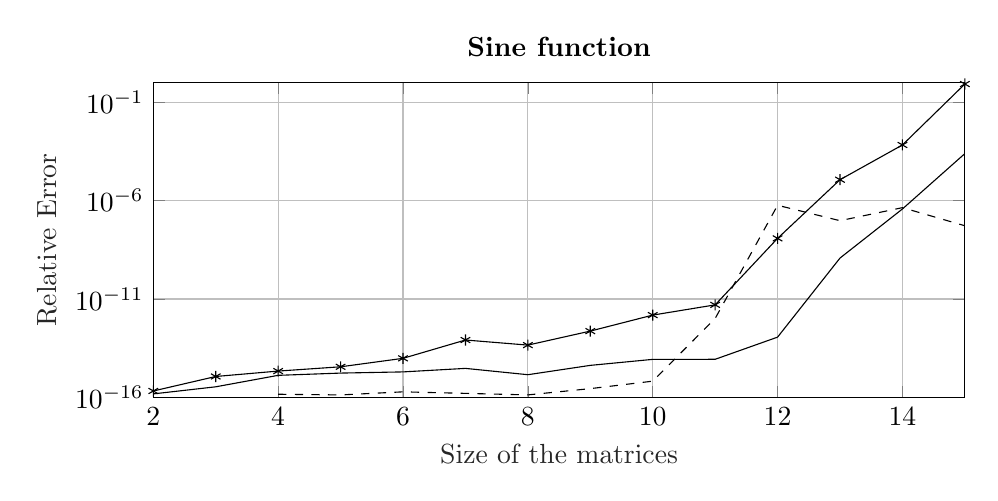
\begin{tikzpicture}

\begin{axis}[%
width=.85\linewidth,
height=4cm,
at={(0in,0in)},
scale only axis,
xmin=2,
xmax=15,
xlabel style={font=\color{white!15!black}},
xlabel={Size of the matrices},
ymode=log,
ymin=1e-16,
ymax=1,
yminorticks=true,
ylabel style={font=\color{white!15!black}},
ylabel={Relative Error},
axis background/.style={fill=white},
title style={font=\bfseries},
title={Sine function},
xmajorgrids,
ymajorgrids,
yminorgrids,
legend style={legend cell align=left, align=left, draw=white!15!black}
]
\addplot [color=black, dashed]
  table[row sep=crcr]{%
1	0\\
2	0\\
3	0\\
4	1.45725786217287e-16\\
5	1.34599448599507e-16\\
6	1.93288933939941e-16\\
7	0\\
8	1.34996517212839e-16\\
9	2.8139452012619e-16\\
10	6.73147337595159e-16\\
11	1.03032779116962e-12\\
12	5.78744177027967e-07\\
13	9.553747250617e-08\\
14	4.39017470636033e-07\\
15	5.28442449627079e-08\\
};
%\addlegendentry{diagonal}

\addplot [color=black, mark=asterisk, mark options={solid, black}]
  table[row sep=crcr]{%
1	0\\
2	2.13550872140361e-16\\
3	1.16425372303465e-15\\
4	2.19221444950359e-15\\
5	3.61672445574946e-15\\
6	9.72750676886519e-15\\
7	8.29608424074529e-14\\
8	4.56885037269095e-14\\
9	2.35417884883477e-13\\
10	1.52796832107972e-12\\
11	5.06284131371555e-12\\
12	1.20831615925066e-08\\
13	1.15240427666526e-05\\
14	0.000671713459124643\\
15	0.837016575460994\\
};
%\addlegendentry{symmetric}

\addplot [color=black]
  table[row sep=crcr]{%
1	0\\
2	1.51944372493216e-16\\
3	3.48056882596735e-16\\
4	1.33057104500803e-15\\
5	1.73250362957786e-15\\
6	1.99001209845091e-15\\
7	3.0020193056546e-15\\
8	1.43307608835298e-15\\
9	4.27119186288929e-15\\
10	8.62089393846284e-15\\
11	8.69296395513068e-15\\
12	1.16168249112529e-13\\
13	1.20836095810293e-09\\
14	3.76245413376949e-07\\
15	0.000244683076230114\\
};
%\addlegendentry{dense}

\end{axis}
\end{tikzpicture}%
        \caption{}
        \label{fig:comp_sine}
    \end{subfigure}\hspace{.055\linewidth}
    \begin{subfigure}[b]{0.3\textwidth}
        % This file was created by matlab2tikz.
%
%The latest updates can be retrieved from
%  http://www.mathworks.com/matlabcentral/fileexchange/22022-matlab2tikz-matlab2tikz
%where you can also make suggestions and rate matlab2tikz.
%
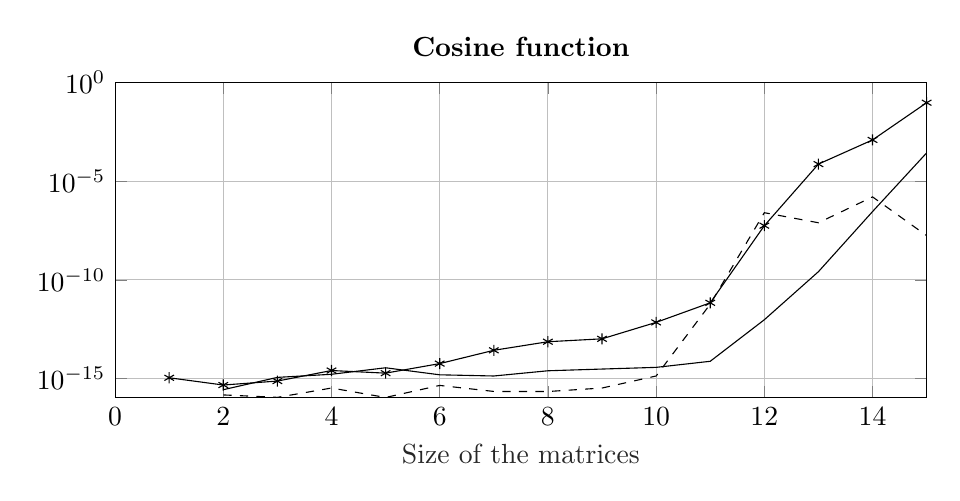
\begin{tikzpicture}

\begin{axis}[%
width=.85\linewidth,
height=4cm,
at={(0in,0in)},
scale only axis,
xmin=0,
xmax=15,
xlabel style={font=\color{white!15!black}},
xlabel={Size of the matrices},
ymode=log,
ymin=1.1104582787894e-16,
ymax=1,
yminorticks=true,
ylabel style={font=\color{white!15!black}},
%ylabel={Relative Error},
axis background/.style={fill=white},
title style={font=\bfseries},
title={Cosine function},
xmajorgrids,
ymajorgrids,
yminorgrids,
legend style={legend cell align=left, align=left, draw=white!15!black}
]
\addplot [color=black, dashed]
  table[row sep=crcr]{%
1	0\\
2	1.49254976159848e-16\\
3	1.12386960222902e-16\\
4	3.33629533162353e-16\\
5	1.1104582787894e-16\\
6	4.51664304824148e-16\\
7	2.24222591598726e-16\\
8	2.22284366724468e-16\\
9	3.3326394200314e-16\\
10	1.35535886136552e-15\\
11	5.90120769250069e-12\\
12	2.53895186073711e-07\\
13	7.86074239881932e-08\\
14	1.60599491859353e-06\\
15	1.74974849891932e-08\\
};
%\addlegendentry{diagonal}

\addplot [color=black, mark=asterisk, mark options={solid, black}]
  table[row sep=crcr]{%
1	1.10216884990089e-15\\
2	4.73392519955033e-16\\
3	7.52201284293378e-16\\
4	2.56983598583253e-15\\
5	1.8934958043445e-15\\
6	5.76079452953616e-15\\
7	2.71936809409104e-14\\
8	7.38660809880766e-14\\
9	1.03575975843225e-13\\
10	7.05810087502504e-13\\
11	6.91539504160167e-12\\
12	5.58866941125034e-08\\
13	7.35834262695204e-05\\
14	0.00123336328753215\\
15	0.0944453153509049\\
};
%\addlegendentry{symmetric}

\addplot [color=black]
  table[row sep=crcr]{%
1	0\\
2	2.74801956341246e-16\\
3	1.15411270860285e-15\\
4	1.65853388726515e-15\\
5	3.54103245149018e-15\\
6	1.5589802910102e-15\\
7	1.35811075119445e-15\\
8	2.49648348011263e-15\\
9	3.05245869225958e-15\\
10	3.71275847951212e-15\\
11	7.54587960659731e-15\\
12	9.59882062625648e-13\\
13	2.61418513595533e-10\\
14	2.89445409507326e-07\\
15	0.000271321657431055\\
};
%\addlegendentry{dense}

\end{axis}
\end{tikzpicture}%
        \caption{}
        \label{fig:comp_cosine}
    \end{subfigure}\hspace{.025\linewidth}
    \begin{subfigure}[b]{0.3\textwidth}
        % This file was created by matlab2tikz.
%
%The latest updates can be retrieved from
%  http://www.mathworks.com/matlabcentral/fileexchange/22022-matlab2tikz-matlab2tikz
%where you can also make suggestions and rate matlab2tikz.
%
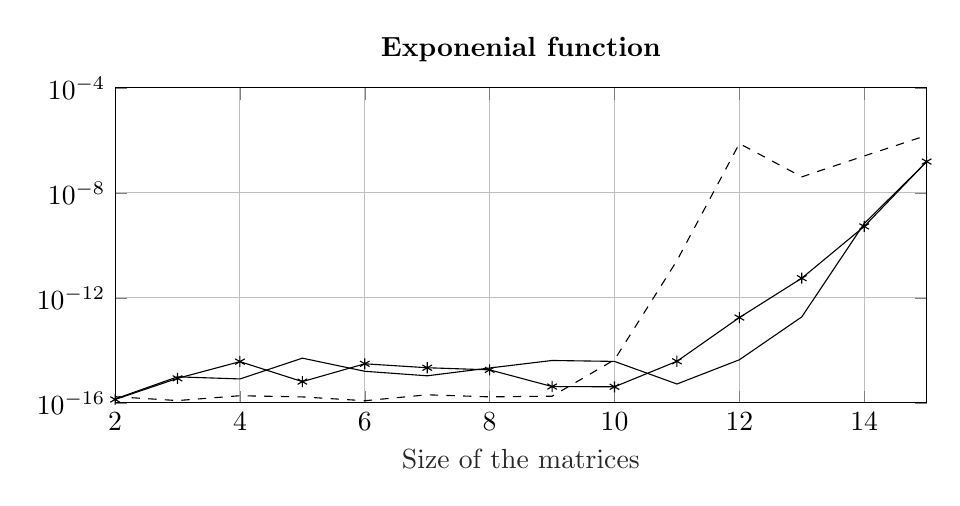
\begin{tikzpicture}

\begin{axis}[%
width=.85\linewidth,
height=4cm,
at={(0in,0in)},
scale only axis,
xmin=2,
xmax=15,
xlabel style={font=\color{white!15!black}},
xlabel={Size of the matrices},
ymode=log,
ymin=1e-16,
ymax=0.0001,
yminorticks=true,
ylabel style={font=\color{white!15!black}},
%ylabel={Relative Error},
axis background/.style={fill=white},
title style={font=\bfseries},
title={Exponenial function},
xmajorgrids,
ymajorgrids,
yminorgrids,
legend style={legend cell align=left, align=left, draw=white!15!black}
]
\addplot [color=black, dashed]
  table[row sep=crcr]{%
1	0\\
2	1.71624878976539e-16\\
3	1.22024250623032e-16\\
4	1.86764659618892e-16\\
5	1.68361863632822e-16\\
6	1.20424787755581e-16\\
7	2.02522198739353e-16\\
8	1.69083627914502e-16\\
9	1.78878188543304e-16\\
10	4.37883232600663e-15\\
11	2.62205407924652e-11\\
12	7.55548252824038e-07\\
13	4.08147804640456e-08\\
14	2.54902728221652e-07\\
15	1.54338995955608e-06\\
};
%\addlegendentry{diagonal}

\addplot [color=black, mark=asterisk, mark options={solid, black}]
  table[row sep=crcr]{%
1	0\\
2	1.34551194988101e-16\\
3	8.56940672084931e-16\\
4	3.71431920865263e-15\\
5	6.43853140792487e-16\\
6	3.07364008605186e-15\\
7	2.17447874006037e-15\\
8	1.80680598636716e-15\\
9	4.18315732440152e-16\\
10	4.08961300873358e-16\\
11	3.83448312676478e-15\\
12	1.77593347794744e-13\\
13	5.61443457608614e-12\\
14	5.25277002444549e-10\\
15	1.55722814732103e-07\\
};
%\addlegendentry{symmetric}

\addplot [color=black]
  table[row sep=crcr]{%
1	0\\
2	1.40422527187022e-16\\
3	9.78212455490046e-16\\
4	8.14581110397033e-16\\
5	5.04209119228841e-15\\
6	1.59210015961528e-15\\
7	1.07228002023245e-15\\
8	2.12873989764519e-15\\
9	4.11404419473943e-15\\
10	3.79263905604626e-15\\
11	5.22236059957374e-16\\
12	4.37354475237039e-15\\
13	1.88271014260457e-13\\
14	6.79585192457534e-10\\
15	1.52106181005324e-07\\
};
%\addlegendentry{dense}

\end{axis}
\end{tikzpicture}%
        \caption{}
        \label{fig:comp_exp}
    \end{subfigure}
    \caption{Measure of performance of the algorithm to compute $f(\mathbf{A})$ according to definition \ref{def:Hermite}. We assume that \cite{davies2003schur} (Schur Parlett) algorithm is correct, and we measure the relative error. We compare the performance of our algorithm on several types of matrices : diagonal (- -), symmetric (-*) and dense (--). Matrix coefficients are randomly filled such that for all non-zero entry: $a_{ij}\sim\mathcal{U}(0,1)$, this ensures $\mathbf{A}$ is full rank. We test it on three different functions : Sine (a), Cosine (b) and Exponenial (c). We note that starting from a certain matrix size, the algorithm lose considerably in performance.}
    \label{fig:comp}
\end{figure}

Figure \ref{fig:comp} illustrates the result of the measurement of performance of the algorithm. The relative error between \cite{davies2003schur} and our results is computed:
\begin{equation*}
    \text{relative error} = \frac{\|f(\mathbf{A})-\texttt{funm}(\mathbf{A},f)\|_2}{\|\texttt{funm}(\mathbf{A},f\|_2}
\end{equation*}
We note that for small matrices ($n\leq 10$), the hermite interpolation approach is precise and has residual error inferior to $10^{-11}$, which is somewhat close to numerical precision (around $10^{-16}$ as we work with double precision). However, starting from a certain matrix size, the algorithm loses considerably in performance: both in precision and in computation time. Interestingly, this behavior is independant to the matrix structure : diagonal, symmetric or dense. It also seem to be independant to the function we are evaluating (though we has slightly lower relative error for the exponential function as depicted in figure \ref{fig:comp_exp}).

We conclude that this algorithm, while being elegant, is quickly inefficient, and lead to both numerical and computational issues, even at small matrix sizes.

\subsection{Matrix-vector product}
\subsubsection{Implementation}
In this section, we will implement the matrix-vector product $f(\mathbf{A})\mathbf{b}$, as described in section \ref{sec:fabintro}. We will use the Arnoldi method to achieve this. The implementation is done in \texttt{Matlab 2023a}. As the theory has been well described in section \ref{sec:fabintro}, the implementation is straight-forward :
\begin{algorithm2e}
    \SetAlgoLined
    \KwData{$\mathbf{A} \in \mathbb{C}^{n \times n}$, $\mathbf{b} \in \mathbb{C}^n$, $f$ a function and $k\in\mathbb{N}$ the dimension of the Krylov subspace}
    \KwResult{$f(\mathbf{A})\mathbf{b}$}
    \caption{Matrix-Vector Product}
    $\mathbf{v}_1 \gets \mathbf{b}/\|\mathbf{b}\|_2$\;
    $[\mathbf{V},\mathbf{H}] \gets$ \texttt{arnoldi}($\mathbf{A},\mathbf{v}_1,k$)\;
    $e_1 \gets$ first column of the identity matrix\;
    $f \gets \|b\|_2\mathbf{V}f(\mathbf{H})\mathbf{e}_1$\;
\end{algorithm2e}

Where \texttt{arnoldi()} is the Arnoldi iteration described in algorithm \ref{alg:arnoldi}. This routine is provided in the supplementary materials.

\subsubsection{Results}
To evaluate the performance of this Matrix-vector product routine, we will test it versus the naive way of doing it in \texttt{Matlab}, meaning computing $f(\mathbf{A})$ explicitely, then multiplying it by $\mathbf{b}$. In our first experiment (figure \ref{fig:comp_fab}), where $\mathbf{A}$ is a large sparse matrix. More specifically it is a graded L-shape pattern from \cite{george1978automatic}. The vector $\mathbf{b}$ is filled with uniformly distributed random coefficients such that $b_i\sim\mathcal{U}(0,1)$. The figure \ref{fig:comp_fab_assignement} shows that for such a setup, the proposed algorithm reaches a relative error equals to numerical precision few iterations afters 20. This means 
\begin{equation*}
    \frac{\|\|\mathbf{b}\|_2\mathbf{V}_k f(\mathbf{H}_k)\mathbf{e}_1 - f(\mathbf{A})\mathbf{b}\|_2}{\|f(\mathbf{A})\mathbf{b}\|_2} = \epsilon
\end{equation*}
for $k > 20$, and where $\epsilon$ is the machine precision. Note that this result is very specific to the problem depicted in figure \ref{fig:comp_fab}, and the threshold for $k$ will differ in function of the considered problem. Another interpretation is that computing $f(\mathbf{A})\mathbf{b}$ on the smaller Krylov subspace $\mathcal{K}_k(\mathbf{A},\mathbf{b})$ gives extremely good results, even when $k << n$. 
\begin{figure}
    \begin{subfigure}[b]{.45\linewidth}
        % This file was created by matlab2tikz.
%
%The latest updates can be retrieved from
%  http://www.mathworks.com/matlabcentral/fileexchange/22022-matlab2tikz-matlab2tikz
%where you can also make suggestions and rate matlab2tikz.
%
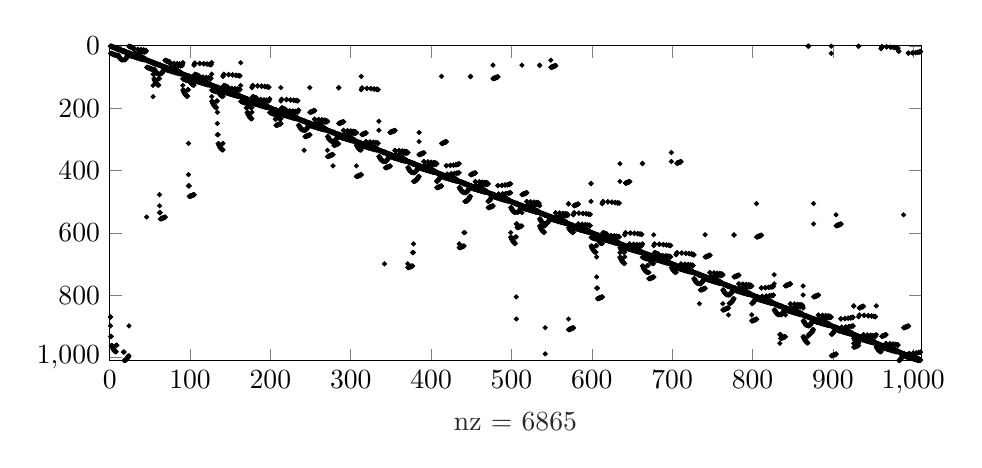
\begin{tikzpicture}

\begin{axis}[%
width=.85\linewidth,
height=4cm,
at={(0in,0in)},
scale only axis,
xmin=0,
xmax=1010,
xlabel style={font=\color{white!15!black}},
xlabel={nz = 6865},
y dir=reverse,
ymin=0,
ymax=1010,
axis background/.style={fill=white},
legend style={legend cell align=left, align=left, draw=white!15!black}
]
\addplot [color=black, draw=none, mark size=0.7pt, mark=*, mark options={solid, black}, forget plot]
  table[row sep=crcr]{%
1	1\\
1	2\\
1	24\\
1	869\\
1	870\\
1	898\\
1	932\\
2	1\\
2	2\\
2	3\\
2	24\\
2	25\\
2	932\\
2	961\\
3	2\\
3	3\\
3	4\\
3	25\\
3	26\\
3	961\\
3	967\\
4	3\\
4	4\\
4	5\\
4	26\\
4	27\\
4	967\\
4	972\\
5	4\\
5	5\\
5	6\\
5	27\\
5	28\\
5	972\\
5	976\\
6	5\\
6	6\\
6	7\\
6	28\\
6	29\\
6	976\\
6	979\\
7	6\\
7	7\\
7	8\\
7	29\\
7	30\\
7	979\\
7	981\\
8	7\\
8	8\\
8	9\\
8	10\\
8	30\\
8	960\\
8	981\\
9	8\\
9	9\\
9	10\\
9	960\\
10	8\\
10	9\\
10	10\\
10	11\\
10	30\\
11	10\\
11	11\\
11	12\\
11	30\\
11	35\\
12	11\\
12	12\\
12	13\\
12	35\\
12	39\\
13	12\\
13	13\\
13	14\\
13	39\\
13	42\\
14	13\\
14	14\\
14	15\\
14	42\\
14	44\\
15	14\\
15	15\\
15	16\\
15	44\\
15	45\\
16	15\\
16	16\\
16	17\\
16	18\\
16	45\\
17	16\\
17	17\\
17	18\\
17	982\\
18	16\\
18	17\\
18	18\\
18	19\\
18	45\\
18	982\\
18	1009\\
19	18\\
19	19\\
19	20\\
19	43\\
19	45\\
19	1008\\
19	1009\\
20	19\\
20	20\\
20	21\\
20	40\\
20	43\\
20	1006\\
20	1008\\
21	20\\
21	21\\
21	22\\
21	36\\
21	40\\
21	1003\\
21	1006\\
22	21\\
22	22\\
22	23\\
22	31\\
22	36\\
22	999\\
22	1003\\
23	22\\
23	23\\
23	24\\
23	25\\
23	31\\
23	994\\
23	999\\
24	1\\
24	2\\
24	23\\
24	24\\
24	25\\
24	898\\
24	994\\
25	2\\
25	3\\
25	23\\
25	24\\
25	25\\
25	26\\
25	31\\
26	3\\
26	4\\
26	25\\
26	26\\
26	27\\
26	31\\
26	32\\
27	4\\
27	5\\
27	26\\
27	27\\
27	28\\
27	32\\
27	33\\
28	5\\
28	6\\
28	27\\
28	28\\
28	29\\
28	33\\
28	34\\
29	6\\
29	7\\
29	28\\
29	29\\
29	30\\
29	34\\
29	35\\
30	7\\
30	8\\
30	10\\
30	11\\
30	29\\
30	30\\
30	35\\
31	22\\
31	23\\
31	25\\
31	26\\
31	31\\
31	32\\
31	36\\
32	26\\
32	27\\
32	31\\
32	32\\
32	33\\
32	36\\
32	37\\
33	27\\
33	28\\
33	32\\
33	33\\
33	34\\
33	37\\
33	38\\
34	28\\
34	29\\
34	33\\
34	34\\
34	35\\
34	38\\
34	39\\
35	11\\
35	12\\
35	29\\
35	30\\
35	34\\
35	35\\
35	39\\
36	21\\
36	22\\
36	31\\
36	32\\
36	36\\
36	37\\
36	40\\
37	32\\
37	33\\
37	36\\
37	37\\
37	38\\
37	40\\
37	41\\
38	33\\
38	34\\
38	37\\
38	38\\
38	39\\
38	41\\
38	42\\
39	12\\
39	13\\
39	34\\
39	35\\
39	38\\
39	39\\
39	42\\
40	20\\
40	21\\
40	36\\
40	37\\
40	40\\
40	41\\
40	43\\
41	37\\
41	38\\
41	40\\
41	41\\
41	42\\
41	43\\
41	44\\
42	13\\
42	14\\
42	38\\
42	39\\
42	41\\
42	42\\
42	44\\
43	19\\
43	20\\
43	40\\
43	41\\
43	43\\
43	44\\
43	45\\
44	14\\
44	15\\
44	41\\
44	42\\
44	43\\
44	44\\
44	45\\
45	15\\
45	16\\
45	18\\
45	19\\
45	43\\
45	44\\
45	45\\
46	46\\
46	47\\
46	69\\
46	549\\
47	46\\
47	47\\
47	48\\
47	69\\
47	70\\
48	47\\
48	48\\
48	49\\
48	70\\
48	71\\
49	48\\
49	49\\
49	50\\
49	71\\
49	72\\
50	49\\
50	50\\
50	51\\
50	72\\
50	73\\
51	50\\
51	51\\
51	52\\
51	73\\
51	74\\
52	51\\
52	52\\
52	53\\
52	74\\
52	75\\
53	52\\
53	53\\
53	54\\
53	55\\
53	75\\
54	53\\
54	54\\
54	55\\
54	91\\
54	127\\
54	163\\
55	53\\
55	54\\
55	55\\
55	56\\
55	75\\
55	91\\
55	106\\
56	55\\
56	56\\
56	57\\
56	75\\
56	80\\
56	106\\
56	112\\
57	56\\
57	57\\
57	58\\
57	80\\
57	84\\
57	112\\
57	117\\
58	57\\
58	58\\
58	59\\
58	84\\
58	87\\
58	117\\
58	121\\
59	58\\
59	59\\
59	60\\
59	87\\
59	89\\
59	121\\
59	124\\
60	59\\
60	60\\
60	61\\
60	89\\
60	90\\
60	124\\
60	126\\
61	60\\
61	61\\
61	62\\
61	63\\
61	90\\
61	105\\
61	126\\
62	61\\
62	62\\
62	63\\
62	105\\
62	477\\
62	513\\
62	535\\
63	61\\
63	62\\
63	63\\
63	64\\
63	90\\
63	535\\
63	555\\
64	63\\
64	64\\
64	65\\
64	88\\
64	90\\
64	554\\
64	555\\
65	64\\
65	65\\
65	66\\
65	85\\
65	88\\
65	553\\
65	554\\
66	65\\
66	66\\
66	67\\
66	81\\
66	85\\
66	552\\
66	553\\
67	66\\
67	67\\
67	68\\
67	76\\
67	81\\
67	551\\
67	552\\
68	67\\
68	68\\
68	69\\
68	70\\
68	76\\
68	550\\
68	551\\
69	46\\
69	47\\
69	68\\
69	69\\
69	70\\
69	549\\
69	550\\
70	47\\
70	48\\
70	68\\
70	69\\
70	70\\
70	71\\
70	76\\
71	48\\
71	49\\
71	70\\
71	71\\
71	72\\
71	76\\
71	77\\
72	49\\
72	50\\
72	71\\
72	72\\
72	73\\
72	77\\
72	78\\
73	50\\
73	51\\
73	72\\
73	73\\
73	74\\
73	78\\
73	79\\
74	51\\
74	52\\
74	73\\
74	74\\
74	75\\
74	79\\
74	80\\
75	52\\
75	53\\
75	55\\
75	56\\
75	74\\
75	75\\
75	80\\
76	67\\
76	68\\
76	70\\
76	71\\
76	76\\
76	77\\
76	81\\
77	71\\
77	72\\
77	76\\
77	77\\
77	78\\
77	81\\
77	82\\
78	72\\
78	73\\
78	77\\
78	78\\
78	79\\
78	82\\
78	83\\
79	73\\
79	74\\
79	78\\
79	79\\
79	80\\
79	83\\
79	84\\
80	56\\
80	57\\
80	74\\
80	75\\
80	79\\
80	80\\
80	84\\
81	66\\
81	67\\
81	76\\
81	77\\
81	81\\
81	82\\
81	85\\
82	77\\
82	78\\
82	81\\
82	82\\
82	83\\
82	85\\
82	86\\
83	78\\
83	79\\
83	82\\
83	83\\
83	84\\
83	86\\
83	87\\
84	57\\
84	58\\
84	79\\
84	80\\
84	83\\
84	84\\
84	87\\
85	65\\
85	66\\
85	81\\
85	82\\
85	85\\
85	86\\
85	88\\
86	82\\
86	83\\
86	85\\
86	86\\
86	87\\
86	88\\
86	89\\
87	58\\
87	59\\
87	83\\
87	84\\
87	86\\
87	87\\
87	89\\
88	64\\
88	65\\
88	85\\
88	86\\
88	88\\
88	89\\
88	90\\
89	59\\
89	60\\
89	86\\
89	87\\
89	88\\
89	89\\
89	90\\
90	60\\
90	61\\
90	63\\
90	64\\
90	88\\
90	89\\
90	90\\
91	54\\
91	55\\
91	91\\
91	92\\
91	106\\
91	127\\
91	142\\
92	91\\
92	92\\
92	93\\
92	106\\
92	107\\
92	142\\
92	148\\
93	92\\
93	93\\
93	94\\
93	107\\
93	108\\
93	148\\
93	153\\
94	93\\
94	94\\
94	95\\
94	108\\
94	109\\
94	153\\
94	157\\
95	94\\
95	95\\
95	96\\
95	109\\
95	110\\
95	157\\
95	160\\
96	95\\
96	96\\
96	97\\
96	110\\
96	111\\
96	160\\
96	162\\
97	96\\
97	97\\
97	98\\
97	99\\
97	111\\
97	141\\
97	162\\
98	97\\
98	98\\
98	99\\
98	141\\
98	313\\
98	413\\
98	449\\
99	97\\
99	98\\
99	99\\
99	100\\
99	111\\
99	449\\
99	483\\
100	99\\
100	100\\
100	101\\
100	111\\
100	116\\
100	482\\
100	483\\
101	100\\
101	101\\
101	102\\
101	116\\
101	120\\
101	481\\
101	482\\
102	101\\
102	102\\
102	103\\
102	120\\
102	123\\
102	480\\
102	481\\
103	102\\
103	103\\
103	104\\
103	123\\
103	125\\
103	479\\
103	480\\
104	103\\
104	104\\
104	105\\
104	125\\
104	126\\
104	478\\
104	479\\
105	61\\
105	62\\
105	104\\
105	105\\
105	126\\
105	477\\
105	478\\
106	55\\
106	56\\
106	91\\
106	92\\
106	106\\
106	107\\
106	112\\
107	92\\
107	93\\
107	106\\
107	107\\
107	108\\
107	112\\
107	113\\
108	93\\
108	94\\
108	107\\
108	108\\
108	109\\
108	113\\
108	114\\
109	94\\
109	95\\
109	108\\
109	109\\
109	110\\
109	114\\
109	115\\
110	95\\
110	96\\
110	109\\
110	110\\
110	111\\
110	115\\
110	116\\
111	96\\
111	97\\
111	99\\
111	100\\
111	110\\
111	111\\
111	116\\
112	56\\
112	57\\
112	106\\
112	107\\
112	112\\
112	113\\
112	117\\
113	107\\
113	108\\
113	112\\
113	113\\
113	114\\
113	117\\
113	118\\
114	108\\
114	109\\
114	113\\
114	114\\
114	115\\
114	118\\
114	119\\
115	109\\
115	110\\
115	114\\
115	115\\
115	116\\
115	119\\
115	120\\
116	100\\
116	101\\
116	110\\
116	111\\
116	115\\
116	116\\
116	120\\
117	57\\
117	58\\
117	112\\
117	113\\
117	117\\
117	118\\
117	121\\
118	113\\
118	114\\
118	117\\
118	118\\
118	119\\
118	121\\
118	122\\
119	114\\
119	115\\
119	118\\
119	119\\
119	120\\
119	122\\
119	123\\
120	101\\
120	102\\
120	115\\
120	116\\
120	119\\
120	120\\
120	123\\
121	58\\
121	59\\
121	117\\
121	118\\
121	121\\
121	122\\
121	124\\
122	118\\
122	119\\
122	121\\
122	122\\
122	123\\
122	124\\
122	125\\
123	102\\
123	103\\
123	119\\
123	120\\
123	122\\
123	123\\
123	125\\
124	59\\
124	60\\
124	121\\
124	122\\
124	124\\
124	125\\
124	126\\
125	103\\
125	104\\
125	122\\
125	123\\
125	124\\
125	125\\
125	126\\
126	60\\
126	61\\
126	104\\
126	105\\
126	124\\
126	125\\
126	126\\
127	54\\
127	91\\
127	127\\
127	128\\
127	142\\
127	163\\
127	178\\
128	127\\
128	128\\
128	129\\
128	142\\
128	143\\
128	178\\
128	184\\
129	128\\
129	129\\
129	130\\
129	143\\
129	144\\
129	184\\
129	189\\
130	129\\
130	130\\
130	131\\
130	144\\
130	145\\
130	189\\
130	193\\
131	130\\
131	131\\
131	132\\
131	145\\
131	146\\
131	193\\
131	196\\
132	131\\
132	132\\
132	133\\
132	146\\
132	147\\
132	196\\
132	198\\
133	132\\
133	133\\
133	134\\
133	135\\
133	147\\
133	177\\
133	198\\
134	133\\
134	134\\
134	135\\
134	177\\
134	213\\
134	249\\
134	285\\
135	133\\
135	134\\
135	135\\
135	136\\
135	147\\
135	285\\
135	314\\
136	135\\
136	136\\
136	137\\
136	147\\
136	152\\
136	314\\
136	320\\
137	136\\
137	137\\
137	138\\
137	152\\
137	156\\
137	320\\
137	325\\
138	137\\
138	138\\
138	139\\
138	156\\
138	159\\
138	325\\
138	329\\
139	138\\
139	139\\
139	140\\
139	159\\
139	161\\
139	329\\
139	332\\
140	139\\
140	140\\
140	141\\
140	161\\
140	162\\
140	332\\
140	334\\
141	97\\
141	98\\
141	140\\
141	141\\
141	162\\
141	313\\
141	334\\
142	91\\
142	92\\
142	127\\
142	128\\
142	142\\
142	143\\
142	148\\
143	128\\
143	129\\
143	142\\
143	143\\
143	144\\
143	148\\
143	149\\
144	129\\
144	130\\
144	143\\
144	144\\
144	145\\
144	149\\
144	150\\
145	130\\
145	131\\
145	144\\
145	145\\
145	146\\
145	150\\
145	151\\
146	131\\
146	132\\
146	145\\
146	146\\
146	147\\
146	151\\
146	152\\
147	132\\
147	133\\
147	135\\
147	136\\
147	146\\
147	147\\
147	152\\
148	92\\
148	93\\
148	142\\
148	143\\
148	148\\
148	149\\
148	153\\
149	143\\
149	144\\
149	148\\
149	149\\
149	150\\
149	153\\
149	154\\
150	144\\
150	145\\
150	149\\
150	150\\
150	151\\
150	154\\
150	155\\
151	145\\
151	146\\
151	150\\
151	151\\
151	152\\
151	155\\
151	156\\
152	136\\
152	137\\
152	146\\
152	147\\
152	151\\
152	152\\
152	156\\
153	93\\
153	94\\
153	148\\
153	149\\
153	153\\
153	154\\
153	157\\
154	149\\
154	150\\
154	153\\
154	154\\
154	155\\
154	157\\
154	158\\
155	150\\
155	151\\
155	154\\
155	155\\
155	156\\
155	158\\
155	159\\
156	137\\
156	138\\
156	151\\
156	152\\
156	155\\
156	156\\
156	159\\
157	94\\
157	95\\
157	153\\
157	154\\
157	157\\
157	158\\
157	160\\
158	154\\
158	155\\
158	157\\
158	158\\
158	159\\
158	160\\
158	161\\
159	138\\
159	139\\
159	155\\
159	156\\
159	158\\
159	159\\
159	161\\
160	95\\
160	96\\
160	157\\
160	158\\
160	160\\
160	161\\
160	162\\
161	139\\
161	140\\
161	158\\
161	159\\
161	160\\
161	161\\
161	162\\
162	96\\
162	97\\
162	140\\
162	141\\
162	160\\
162	161\\
162	162\\
163	54\\
163	127\\
163	163\\
163	164\\
163	178\\
164	163\\
164	164\\
164	165\\
164	178\\
164	179\\
165	164\\
165	165\\
165	166\\
165	179\\
165	180\\
166	165\\
166	166\\
166	167\\
166	180\\
166	181\\
167	166\\
167	167\\
167	168\\
167	181\\
167	182\\
168	167\\
168	168\\
168	169\\
168	182\\
168	183\\
169	168\\
169	169\\
169	170\\
169	171\\
169	183\\
170	169\\
170	170\\
170	171\\
170	199\\
171	169\\
171	170\\
171	171\\
171	172\\
171	183\\
171	199\\
171	214\\
172	171\\
172	172\\
172	173\\
172	183\\
172	188\\
172	214\\
172	220\\
173	172\\
173	173\\
173	174\\
173	188\\
173	192\\
173	220\\
173	225\\
174	173\\
174	174\\
174	175\\
174	192\\
174	195\\
174	225\\
174	229\\
175	174\\
175	175\\
175	176\\
175	195\\
175	197\\
175	229\\
175	232\\
176	175\\
176	176\\
176	177\\
176	197\\
176	198\\
176	232\\
176	234\\
177	133\\
177	134\\
177	176\\
177	177\\
177	198\\
177	213\\
177	234\\
178	127\\
178	128\\
178	163\\
178	164\\
178	178\\
178	179\\
178	184\\
179	164\\
179	165\\
179	178\\
179	179\\
179	180\\
179	184\\
179	185\\
180	165\\
180	166\\
180	179\\
180	180\\
180	181\\
180	185\\
180	186\\
181	166\\
181	167\\
181	180\\
181	181\\
181	182\\
181	186\\
181	187\\
182	167\\
182	168\\
182	181\\
182	182\\
182	183\\
182	187\\
182	188\\
183	168\\
183	169\\
183	171\\
183	172\\
183	182\\
183	183\\
183	188\\
184	128\\
184	129\\
184	178\\
184	179\\
184	184\\
184	185\\
184	189\\
185	179\\
185	180\\
185	184\\
185	185\\
185	186\\
185	189\\
185	190\\
186	180\\
186	181\\
186	185\\
186	186\\
186	187\\
186	190\\
186	191\\
187	181\\
187	182\\
187	186\\
187	187\\
187	188\\
187	191\\
187	192\\
188	172\\
188	173\\
188	182\\
188	183\\
188	187\\
188	188\\
188	192\\
189	129\\
189	130\\
189	184\\
189	185\\
189	189\\
189	190\\
189	193\\
190	185\\
190	186\\
190	189\\
190	190\\
190	191\\
190	193\\
190	194\\
191	186\\
191	187\\
191	190\\
191	191\\
191	192\\
191	194\\
191	195\\
192	173\\
192	174\\
192	187\\
192	188\\
192	191\\
192	192\\
192	195\\
193	130\\
193	131\\
193	189\\
193	190\\
193	193\\
193	194\\
193	196\\
194	190\\
194	191\\
194	193\\
194	194\\
194	195\\
194	196\\
194	197\\
195	174\\
195	175\\
195	191\\
195	192\\
195	194\\
195	195\\
195	197\\
196	131\\
196	132\\
196	193\\
196	194\\
196	196\\
196	197\\
196	198\\
197	175\\
197	176\\
197	194\\
197	195\\
197	196\\
197	197\\
197	198\\
198	132\\
198	133\\
198	176\\
198	177\\
198	196\\
198	197\\
198	198\\
199	170\\
199	171\\
199	199\\
199	200\\
199	214\\
200	199\\
200	200\\
200	201\\
200	214\\
200	215\\
201	200\\
201	201\\
201	202\\
201	215\\
201	216\\
202	201\\
202	202\\
202	203\\
202	216\\
202	217\\
203	202\\
203	203\\
203	204\\
203	217\\
203	218\\
204	203\\
204	204\\
204	205\\
204	218\\
204	219\\
205	204\\
205	205\\
205	206\\
205	207\\
205	219\\
206	205\\
206	206\\
206	207\\
206	235\\
207	205\\
207	206\\
207	207\\
207	208\\
207	219\\
207	235\\
207	255\\
208	207\\
208	208\\
208	209\\
208	219\\
208	224\\
208	254\\
208	255\\
209	208\\
209	209\\
209	210\\
209	224\\
209	228\\
209	253\\
209	254\\
210	209\\
210	210\\
210	211\\
210	228\\
210	231\\
210	252\\
210	253\\
211	210\\
211	211\\
211	212\\
211	231\\
211	233\\
211	251\\
211	252\\
212	211\\
212	212\\
212	213\\
212	233\\
212	234\\
212	250\\
212	251\\
213	134\\
213	177\\
213	212\\
213	213\\
213	234\\
213	249\\
213	250\\
214	171\\
214	172\\
214	199\\
214	200\\
214	214\\
214	215\\
214	220\\
215	200\\
215	201\\
215	214\\
215	215\\
215	216\\
215	220\\
215	221\\
216	201\\
216	202\\
216	215\\
216	216\\
216	217\\
216	221\\
216	222\\
217	202\\
217	203\\
217	216\\
217	217\\
217	218\\
217	222\\
217	223\\
218	203\\
218	204\\
218	217\\
218	218\\
218	219\\
218	223\\
218	224\\
219	204\\
219	205\\
219	207\\
219	208\\
219	218\\
219	219\\
219	224\\
220	172\\
220	173\\
220	214\\
220	215\\
220	220\\
220	221\\
220	225\\
221	215\\
221	216\\
221	220\\
221	221\\
221	222\\
221	225\\
221	226\\
222	216\\
222	217\\
222	221\\
222	222\\
222	223\\
222	226\\
222	227\\
223	217\\
223	218\\
223	222\\
223	223\\
223	224\\
223	227\\
223	228\\
224	208\\
224	209\\
224	218\\
224	219\\
224	223\\
224	224\\
224	228\\
225	173\\
225	174\\
225	220\\
225	221\\
225	225\\
225	226\\
225	229\\
226	221\\
226	222\\
226	225\\
226	226\\
226	227\\
226	229\\
226	230\\
227	222\\
227	223\\
227	226\\
227	227\\
227	228\\
227	230\\
227	231\\
228	209\\
228	210\\
228	223\\
228	224\\
228	227\\
228	228\\
228	231\\
229	174\\
229	175\\
229	225\\
229	226\\
229	229\\
229	230\\
229	232\\
230	226\\
230	227\\
230	229\\
230	230\\
230	231\\
230	232\\
230	233\\
231	210\\
231	211\\
231	227\\
231	228\\
231	230\\
231	231\\
231	233\\
232	175\\
232	176\\
232	229\\
232	230\\
232	232\\
232	233\\
232	234\\
233	211\\
233	212\\
233	230\\
233	231\\
233	232\\
233	233\\
233	234\\
234	176\\
234	177\\
234	212\\
234	213\\
234	232\\
234	233\\
234	234\\
235	206\\
235	207\\
235	235\\
235	236\\
235	255\\
236	235\\
236	236\\
236	237\\
236	255\\
236	260\\
237	236\\
237	237\\
237	238\\
237	260\\
237	264\\
238	237\\
238	238\\
238	239\\
238	264\\
238	267\\
239	238\\
239	239\\
239	240\\
239	267\\
239	269\\
240	239\\
240	240\\
240	241\\
240	269\\
240	270\\
241	240\\
241	241\\
241	242\\
241	243\\
241	270\\
242	241\\
242	242\\
242	243\\
242	271\\
242	335\\
243	241\\
243	242\\
243	243\\
243	244\\
243	270\\
243	271\\
243	291\\
244	243\\
244	244\\
244	245\\
244	268\\
244	270\\
244	290\\
244	291\\
245	244\\
245	245\\
245	246\\
245	265\\
245	268\\
245	289\\
245	290\\
246	245\\
246	246\\
246	247\\
246	261\\
246	265\\
246	288\\
246	289\\
247	246\\
247	247\\
247	248\\
247	256\\
247	261\\
247	287\\
247	288\\
248	247\\
248	248\\
248	249\\
248	250\\
248	256\\
248	286\\
248	287\\
249	134\\
249	213\\
249	248\\
249	249\\
249	250\\
249	285\\
249	286\\
250	212\\
250	213\\
250	248\\
250	249\\
250	250\\
250	251\\
250	256\\
251	211\\
251	212\\
251	250\\
251	251\\
251	252\\
251	256\\
251	257\\
252	210\\
252	211\\
252	251\\
252	252\\
252	253\\
252	257\\
252	258\\
253	209\\
253	210\\
253	252\\
253	253\\
253	254\\
253	258\\
253	259\\
254	208\\
254	209\\
254	253\\
254	254\\
254	255\\
254	259\\
254	260\\
255	207\\
255	208\\
255	235\\
255	236\\
255	254\\
255	255\\
255	260\\
256	247\\
256	248\\
256	250\\
256	251\\
256	256\\
256	257\\
256	261\\
257	251\\
257	252\\
257	256\\
257	257\\
257	258\\
257	261\\
257	262\\
258	252\\
258	253\\
258	257\\
258	258\\
258	259\\
258	262\\
258	263\\
259	253\\
259	254\\
259	258\\
259	259\\
259	260\\
259	263\\
259	264\\
260	236\\
260	237\\
260	254\\
260	255\\
260	259\\
260	260\\
260	264\\
261	246\\
261	247\\
261	256\\
261	257\\
261	261\\
261	262\\
261	265\\
262	257\\
262	258\\
262	261\\
262	262\\
262	263\\
262	265\\
262	266\\
263	258\\
263	259\\
263	262\\
263	263\\
263	264\\
263	266\\
263	267\\
264	237\\
264	238\\
264	259\\
264	260\\
264	263\\
264	264\\
264	267\\
265	245\\
265	246\\
265	261\\
265	262\\
265	265\\
265	266\\
265	268\\
266	262\\
266	263\\
266	265\\
266	266\\
266	267\\
266	268\\
266	269\\
267	238\\
267	239\\
267	263\\
267	264\\
267	266\\
267	267\\
267	269\\
268	244\\
268	245\\
268	265\\
268	266\\
268	268\\
268	269\\
268	270\\
269	239\\
269	240\\
269	266\\
269	267\\
269	268\\
269	269\\
269	270\\
270	240\\
270	241\\
270	243\\
270	244\\
270	268\\
270	269\\
270	270\\
271	242\\
271	243\\
271	271\\
271	272\\
271	291\\
271	335\\
271	355\\
272	271\\
272	272\\
272	273\\
272	291\\
272	296\\
272	354\\
272	355\\
273	272\\
273	273\\
273	274\\
273	296\\
273	300\\
273	353\\
273	354\\
274	273\\
274	274\\
274	275\\
274	300\\
274	303\\
274	352\\
274	353\\
275	274\\
275	275\\
275	276\\
275	303\\
275	305\\
275	351\\
275	352\\
276	275\\
276	276\\
276	277\\
276	305\\
276	306\\
276	350\\
276	351\\
277	276\\
277	277\\
277	278\\
277	279\\
277	306\\
277	349\\
277	350\\
278	277\\
278	278\\
278	279\\
278	307\\
278	349\\
278	385\\
279	277\\
279	278\\
279	279\\
279	280\\
279	306\\
279	307\\
279	319\\
280	279\\
280	280\\
280	281\\
280	304\\
280	306\\
280	318\\
280	319\\
281	280\\
281	281\\
281	282\\
281	301\\
281	304\\
281	317\\
281	318\\
282	281\\
282	282\\
282	283\\
282	297\\
282	301\\
282	316\\
282	317\\
283	282\\
283	283\\
283	284\\
283	292\\
283	297\\
283	315\\
283	316\\
284	283\\
284	284\\
284	285\\
284	286\\
284	292\\
284	314\\
284	315\\
285	134\\
285	135\\
285	249\\
285	284\\
285	285\\
285	286\\
285	314\\
286	248\\
286	249\\
286	284\\
286	285\\
286	286\\
286	287\\
286	292\\
287	247\\
287	248\\
287	286\\
287	287\\
287	288\\
287	292\\
287	293\\
288	246\\
288	247\\
288	287\\
288	288\\
288	289\\
288	293\\
288	294\\
289	245\\
289	246\\
289	288\\
289	289\\
289	290\\
289	294\\
289	295\\
290	244\\
290	245\\
290	289\\
290	290\\
290	291\\
290	295\\
290	296\\
291	243\\
291	244\\
291	271\\
291	272\\
291	290\\
291	291\\
291	296\\
292	283\\
292	284\\
292	286\\
292	287\\
292	292\\
292	293\\
292	297\\
293	287\\
293	288\\
293	292\\
293	293\\
293	294\\
293	297\\
293	298\\
294	288\\
294	289\\
294	293\\
294	294\\
294	295\\
294	298\\
294	299\\
295	289\\
295	290\\
295	294\\
295	295\\
295	296\\
295	299\\
295	300\\
296	272\\
296	273\\
296	290\\
296	291\\
296	295\\
296	296\\
296	300\\
297	282\\
297	283\\
297	292\\
297	293\\
297	297\\
297	298\\
297	301\\
298	293\\
298	294\\
298	297\\
298	298\\
298	299\\
298	301\\
298	302\\
299	294\\
299	295\\
299	298\\
299	299\\
299	300\\
299	302\\
299	303\\
300	273\\
300	274\\
300	295\\
300	296\\
300	299\\
300	300\\
300	303\\
301	281\\
301	282\\
301	297\\
301	298\\
301	301\\
301	302\\
301	304\\
302	298\\
302	299\\
302	301\\
302	302\\
302	303\\
302	304\\
302	305\\
303	274\\
303	275\\
303	299\\
303	300\\
303	302\\
303	303\\
303	305\\
304	280\\
304	281\\
304	301\\
304	302\\
304	304\\
304	305\\
304	306\\
305	275\\
305	276\\
305	302\\
305	303\\
305	304\\
305	305\\
305	306\\
306	276\\
306	277\\
306	279\\
306	280\\
306	304\\
306	305\\
306	306\\
307	278\\
307	279\\
307	307\\
307	308\\
307	319\\
307	385\\
307	419\\
308	307\\
308	308\\
308	309\\
308	319\\
308	324\\
308	418\\
308	419\\
309	308\\
309	309\\
309	310\\
309	324\\
309	328\\
309	417\\
309	418\\
310	309\\
310	310\\
310	311\\
310	328\\
310	331\\
310	416\\
310	417\\
311	310\\
311	311\\
311	312\\
311	331\\
311	333\\
311	415\\
311	416\\
312	311\\
312	312\\
312	313\\
312	333\\
312	334\\
312	414\\
312	415\\
313	98\\
313	141\\
313	312\\
313	313\\
313	334\\
313	413\\
313	414\\
314	135\\
314	136\\
314	284\\
314	285\\
314	314\\
314	315\\
314	320\\
315	283\\
315	284\\
315	314\\
315	315\\
315	316\\
315	320\\
315	321\\
316	282\\
316	283\\
316	315\\
316	316\\
316	317\\
316	321\\
316	322\\
317	281\\
317	282\\
317	316\\
317	317\\
317	318\\
317	322\\
317	323\\
318	280\\
318	281\\
318	317\\
318	318\\
318	319\\
318	323\\
318	324\\
319	279\\
319	280\\
319	307\\
319	308\\
319	318\\
319	319\\
319	324\\
320	136\\
320	137\\
320	314\\
320	315\\
320	320\\
320	321\\
320	325\\
321	315\\
321	316\\
321	320\\
321	321\\
321	322\\
321	325\\
321	326\\
322	316\\
322	317\\
322	321\\
322	322\\
322	323\\
322	326\\
322	327\\
323	317\\
323	318\\
323	322\\
323	323\\
323	324\\
323	327\\
323	328\\
324	308\\
324	309\\
324	318\\
324	319\\
324	323\\
324	324\\
324	328\\
325	137\\
325	138\\
325	320\\
325	321\\
325	325\\
325	326\\
325	329\\
326	321\\
326	322\\
326	325\\
326	326\\
326	327\\
326	329\\
326	330\\
327	322\\
327	323\\
327	326\\
327	327\\
327	328\\
327	330\\
327	331\\
328	309\\
328	310\\
328	323\\
328	324\\
328	327\\
328	328\\
328	331\\
329	138\\
329	139\\
329	325\\
329	326\\
329	329\\
329	330\\
329	332\\
330	326\\
330	327\\
330	329\\
330	330\\
330	331\\
330	332\\
330	333\\
331	310\\
331	311\\
331	327\\
331	328\\
331	330\\
331	331\\
331	333\\
332	139\\
332	140\\
332	329\\
332	330\\
332	332\\
332	333\\
332	334\\
333	311\\
333	312\\
333	330\\
333	331\\
333	332\\
333	333\\
333	334\\
334	140\\
334	141\\
334	312\\
334	313\\
334	332\\
334	333\\
334	334\\
335	242\\
335	271\\
335	335\\
335	336\\
335	355\\
336	335\\
336	336\\
336	337\\
336	355\\
336	360\\
337	336\\
337	337\\
337	338\\
337	360\\
337	364\\
338	337\\
338	338\\
338	339\\
338	364\\
338	367\\
339	338\\
339	339\\
339	340\\
339	367\\
339	369\\
340	339\\
340	340\\
340	341\\
340	369\\
340	370\\
341	340\\
341	341\\
341	342\\
341	343\\
341	370\\
342	341\\
342	342\\
342	343\\
342	371\\
342	699\\
343	341\\
343	342\\
343	343\\
343	344\\
343	370\\
343	371\\
343	391\\
344	343\\
344	344\\
344	345\\
344	368\\
344	370\\
344	390\\
344	391\\
345	344\\
345	345\\
345	346\\
345	365\\
345	368\\
345	389\\
345	390\\
346	345\\
346	346\\
346	347\\
346	361\\
346	365\\
346	388\\
346	389\\
347	346\\
347	347\\
347	348\\
347	356\\
347	361\\
347	387\\
347	388\\
348	347\\
348	348\\
348	349\\
348	350\\
348	356\\
348	386\\
348	387\\
349	277\\
349	278\\
349	348\\
349	349\\
349	350\\
349	385\\
349	386\\
350	276\\
350	277\\
350	348\\
350	349\\
350	350\\
350	351\\
350	356\\
351	275\\
351	276\\
351	350\\
351	351\\
351	352\\
351	356\\
351	357\\
352	274\\
352	275\\
352	351\\
352	352\\
352	353\\
352	357\\
352	358\\
353	273\\
353	274\\
353	352\\
353	353\\
353	354\\
353	358\\
353	359\\
354	272\\
354	273\\
354	353\\
354	354\\
354	355\\
354	359\\
354	360\\
355	271\\
355	272\\
355	335\\
355	336\\
355	354\\
355	355\\
355	360\\
356	347\\
356	348\\
356	350\\
356	351\\
356	356\\
356	357\\
356	361\\
357	351\\
357	352\\
357	356\\
357	357\\
357	358\\
357	361\\
357	362\\
358	352\\
358	353\\
358	357\\
358	358\\
358	359\\
358	362\\
358	363\\
359	353\\
359	354\\
359	358\\
359	359\\
359	360\\
359	363\\
359	364\\
360	336\\
360	337\\
360	354\\
360	355\\
360	359\\
360	360\\
360	364\\
361	346\\
361	347\\
361	356\\
361	357\\
361	361\\
361	362\\
361	365\\
362	357\\
362	358\\
362	361\\
362	362\\
362	363\\
362	365\\
362	366\\
363	358\\
363	359\\
363	362\\
363	363\\
363	364\\
363	366\\
363	367\\
364	337\\
364	338\\
364	359\\
364	360\\
364	363\\
364	364\\
364	367\\
365	345\\
365	346\\
365	361\\
365	362\\
365	365\\
365	366\\
365	368\\
366	362\\
366	363\\
366	365\\
366	366\\
366	367\\
366	368\\
366	369\\
367	338\\
367	339\\
367	363\\
367	364\\
367	366\\
367	367\\
367	369\\
368	344\\
368	345\\
368	365\\
368	366\\
368	368\\
368	369\\
368	370\\
369	339\\
369	340\\
369	366\\
369	367\\
369	368\\
369	369\\
369	370\\
370	340\\
370	341\\
370	343\\
370	344\\
370	368\\
370	369\\
370	370\\
371	342\\
371	343\\
371	371\\
371	372\\
371	391\\
371	699\\
371	711\\
372	371\\
372	372\\
372	373\\
372	391\\
372	396\\
372	710\\
372	711\\
373	372\\
373	373\\
373	374\\
373	396\\
373	400\\
373	709\\
373	710\\
374	373\\
374	374\\
374	375\\
374	400\\
374	403\\
374	708\\
374	709\\
375	374\\
375	375\\
375	376\\
375	403\\
375	405\\
375	707\\
375	708\\
376	375\\
376	376\\
376	377\\
376	405\\
376	406\\
376	706\\
376	707\\
377	376\\
377	377\\
377	378\\
377	379\\
377	406\\
377	663\\
377	706\\
378	377\\
378	378\\
378	379\\
378	407\\
378	435\\
378	635\\
378	663\\
379	377\\
379	378\\
379	379\\
379	380\\
379	406\\
379	407\\
379	434\\
380	379\\
380	380\\
380	381\\
380	404\\
380	406\\
380	433\\
380	434\\
381	380\\
381	381\\
381	382\\
381	401\\
381	404\\
381	431\\
381	433\\
382	381\\
382	382\\
382	383\\
382	397\\
382	401\\
382	428\\
382	431\\
383	382\\
383	383\\
383	384\\
383	392\\
383	397\\
383	424\\
383	428\\
384	383\\
384	384\\
384	385\\
384	386\\
384	392\\
384	419\\
384	424\\
385	278\\
385	307\\
385	349\\
385	384\\
385	385\\
385	386\\
385	419\\
386	348\\
386	349\\
386	384\\
386	385\\
386	386\\
386	387\\
386	392\\
387	347\\
387	348\\
387	386\\
387	387\\
387	388\\
387	392\\
387	393\\
388	346\\
388	347\\
388	387\\
388	388\\
388	389\\
388	393\\
388	394\\
389	345\\
389	346\\
389	388\\
389	389\\
389	390\\
389	394\\
389	395\\
390	344\\
390	345\\
390	389\\
390	390\\
390	391\\
390	395\\
390	396\\
391	343\\
391	344\\
391	371\\
391	372\\
391	390\\
391	391\\
391	396\\
392	383\\
392	384\\
392	386\\
392	387\\
392	392\\
392	393\\
392	397\\
393	387\\
393	388\\
393	392\\
393	393\\
393	394\\
393	397\\
393	398\\
394	388\\
394	389\\
394	393\\
394	394\\
394	395\\
394	398\\
394	399\\
395	389\\
395	390\\
395	394\\
395	395\\
395	396\\
395	399\\
395	400\\
396	372\\
396	373\\
396	390\\
396	391\\
396	395\\
396	396\\
396	400\\
397	382\\
397	383\\
397	392\\
397	393\\
397	397\\
397	398\\
397	401\\
398	393\\
398	394\\
398	397\\
398	398\\
398	399\\
398	401\\
398	402\\
399	394\\
399	395\\
399	398\\
399	399\\
399	400\\
399	402\\
399	403\\
400	373\\
400	374\\
400	395\\
400	396\\
400	399\\
400	400\\
400	403\\
401	381\\
401	382\\
401	397\\
401	398\\
401	401\\
401	402\\
401	404\\
402	398\\
402	399\\
402	401\\
402	402\\
402	403\\
402	404\\
402	405\\
403	374\\
403	375\\
403	399\\
403	400\\
403	402\\
403	403\\
403	405\\
404	380\\
404	381\\
404	401\\
404	402\\
404	404\\
404	405\\
404	406\\
405	375\\
405	376\\
405	402\\
405	403\\
405	404\\
405	405\\
405	406\\
406	376\\
406	377\\
406	379\\
406	380\\
406	404\\
406	405\\
406	406\\
407	378\\
407	379\\
407	407\\
407	408\\
407	434\\
407	435\\
407	455\\
408	407\\
408	408\\
408	409\\
408	432\\
408	434\\
408	454\\
408	455\\
409	408\\
409	409\\
409	410\\
409	429\\
409	432\\
409	453\\
409	454\\
410	409\\
410	410\\
410	411\\
410	425\\
410	429\\
410	452\\
410	453\\
411	410\\
411	411\\
411	412\\
411	420\\
411	425\\
411	451\\
411	452\\
412	411\\
412	412\\
412	413\\
412	414\\
412	420\\
412	450\\
412	451\\
413	98\\
413	313\\
413	412\\
413	413\\
413	414\\
413	449\\
413	450\\
414	312\\
414	313\\
414	412\\
414	413\\
414	414\\
414	415\\
414	420\\
415	311\\
415	312\\
415	414\\
415	415\\
415	416\\
415	420\\
415	421\\
416	310\\
416	311\\
416	415\\
416	416\\
416	417\\
416	421\\
416	422\\
417	309\\
417	310\\
417	416\\
417	417\\
417	418\\
417	422\\
417	423\\
418	308\\
418	309\\
418	417\\
418	418\\
418	419\\
418	423\\
418	424\\
419	307\\
419	308\\
419	384\\
419	385\\
419	418\\
419	419\\
419	424\\
420	411\\
420	412\\
420	414\\
420	415\\
420	420\\
420	421\\
420	425\\
421	415\\
421	416\\
421	420\\
421	421\\
421	422\\
421	425\\
421	426\\
422	416\\
422	417\\
422	421\\
422	422\\
422	423\\
422	426\\
422	427\\
423	417\\
423	418\\
423	422\\
423	423\\
423	424\\
423	427\\
423	428\\
424	383\\
424	384\\
424	418\\
424	419\\
424	423\\
424	424\\
424	428\\
425	410\\
425	411\\
425	420\\
425	421\\
425	425\\
425	426\\
425	429\\
426	421\\
426	422\\
426	425\\
426	426\\
426	427\\
426	429\\
426	430\\
427	422\\
427	423\\
427	426\\
427	427\\
427	428\\
427	430\\
427	431\\
428	382\\
428	383\\
428	423\\
428	424\\
428	427\\
428	428\\
428	431\\
429	409\\
429	410\\
429	425\\
429	426\\
429	429\\
429	430\\
429	432\\
430	426\\
430	427\\
430	429\\
430	430\\
430	431\\
430	432\\
430	433\\
431	381\\
431	382\\
431	427\\
431	428\\
431	430\\
431	431\\
431	433\\
432	408\\
432	409\\
432	429\\
432	430\\
432	432\\
432	433\\
432	434\\
433	380\\
433	381\\
433	430\\
433	431\\
433	432\\
433	433\\
433	434\\
434	379\\
434	380\\
434	407\\
434	408\\
434	432\\
434	433\\
434	434\\
435	378\\
435	407\\
435	435\\
435	436\\
435	455\\
435	635\\
435	647\\
436	435\\
436	436\\
436	437\\
436	455\\
436	460\\
436	646\\
436	647\\
437	436\\
437	437\\
437	438\\
437	460\\
437	464\\
437	645\\
437	646\\
438	437\\
438	438\\
438	439\\
438	464\\
438	467\\
438	644\\
438	645\\
439	438\\
439	439\\
439	440\\
439	467\\
439	469\\
439	643\\
439	644\\
440	439\\
440	440\\
440	441\\
440	469\\
440	470\\
440	642\\
440	643\\
441	440\\
441	441\\
441	442\\
441	443\\
441	470\\
441	599\\
441	642\\
442	441\\
442	442\\
442	443\\
442	471\\
442	499\\
442	599\\
443	441\\
443	442\\
443	443\\
443	444\\
443	470\\
443	471\\
443	498\\
444	443\\
444	444\\
444	445\\
444	468\\
444	470\\
444	497\\
444	498\\
445	444\\
445	445\\
445	446\\
445	465\\
445	468\\
445	495\\
445	497\\
446	445\\
446	446\\
446	447\\
446	461\\
446	465\\
446	492\\
446	495\\
447	446\\
447	447\\
447	448\\
447	456\\
447	461\\
447	488\\
447	492\\
448	447\\
448	448\\
448	449\\
448	450\\
448	456\\
448	483\\
448	488\\
449	98\\
449	99\\
449	413\\
449	448\\
449	449\\
449	450\\
449	483\\
450	412\\
450	413\\
450	448\\
450	449\\
450	450\\
450	451\\
450	456\\
451	411\\
451	412\\
451	450\\
451	451\\
451	452\\
451	456\\
451	457\\
452	410\\
452	411\\
452	451\\
452	452\\
452	453\\
452	457\\
452	458\\
453	409\\
453	410\\
453	452\\
453	453\\
453	454\\
453	458\\
453	459\\
454	408\\
454	409\\
454	453\\
454	454\\
454	455\\
454	459\\
454	460\\
455	407\\
455	408\\
455	435\\
455	436\\
455	454\\
455	455\\
455	460\\
456	447\\
456	448\\
456	450\\
456	451\\
456	456\\
456	457\\
456	461\\
457	451\\
457	452\\
457	456\\
457	457\\
457	458\\
457	461\\
457	462\\
458	452\\
458	453\\
458	457\\
458	458\\
458	459\\
458	462\\
458	463\\
459	453\\
459	454\\
459	458\\
459	459\\
459	460\\
459	463\\
459	464\\
460	436\\
460	437\\
460	454\\
460	455\\
460	459\\
460	460\\
460	464\\
461	446\\
461	447\\
461	456\\
461	457\\
461	461\\
461	462\\
461	465\\
462	457\\
462	458\\
462	461\\
462	462\\
462	463\\
462	465\\
462	466\\
463	458\\
463	459\\
463	462\\
463	463\\
463	464\\
463	466\\
463	467\\
464	437\\
464	438\\
464	459\\
464	460\\
464	463\\
464	464\\
464	467\\
465	445\\
465	446\\
465	461\\
465	462\\
465	465\\
465	466\\
465	468\\
466	462\\
466	463\\
466	465\\
466	466\\
466	467\\
466	468\\
466	469\\
467	438\\
467	439\\
467	463\\
467	464\\
467	466\\
467	467\\
467	469\\
468	444\\
468	445\\
468	465\\
468	466\\
468	468\\
468	469\\
468	470\\
469	439\\
469	440\\
469	466\\
469	467\\
469	468\\
469	469\\
469	470\\
470	440\\
470	441\\
470	443\\
470	444\\
470	468\\
470	469\\
470	470\\
471	442\\
471	443\\
471	471\\
471	472\\
471	498\\
471	499\\
471	519\\
472	471\\
472	472\\
472	473\\
472	496\\
472	498\\
472	518\\
472	519\\
473	472\\
473	473\\
473	474\\
473	493\\
473	496\\
473	517\\
473	518\\
474	473\\
474	474\\
474	475\\
474	489\\
474	493\\
474	516\\
474	517\\
475	474\\
475	475\\
475	476\\
475	484\\
475	489\\
475	515\\
475	516\\
476	475\\
476	476\\
476	477\\
476	478\\
476	484\\
476	514\\
476	515\\
477	62\\
477	105\\
477	476\\
477	477\\
477	478\\
477	513\\
477	514\\
478	104\\
478	105\\
478	476\\
478	477\\
478	478\\
478	479\\
478	484\\
479	103\\
479	104\\
479	478\\
479	479\\
479	480\\
479	484\\
479	485\\
480	102\\
480	103\\
480	479\\
480	480\\
480	481\\
480	485\\
480	486\\
481	101\\
481	102\\
481	480\\
481	481\\
481	482\\
481	486\\
481	487\\
482	100\\
482	101\\
482	481\\
482	482\\
482	483\\
482	487\\
482	488\\
483	99\\
483	100\\
483	448\\
483	449\\
483	482\\
483	483\\
483	488\\
484	475\\
484	476\\
484	478\\
484	479\\
484	484\\
484	485\\
484	489\\
485	479\\
485	480\\
485	484\\
485	485\\
485	486\\
485	489\\
485	490\\
486	480\\
486	481\\
486	485\\
486	486\\
486	487\\
486	490\\
486	491\\
487	481\\
487	482\\
487	486\\
487	487\\
487	488\\
487	491\\
487	492\\
488	447\\
488	448\\
488	482\\
488	483\\
488	487\\
488	488\\
488	492\\
489	474\\
489	475\\
489	484\\
489	485\\
489	489\\
489	490\\
489	493\\
490	485\\
490	486\\
490	489\\
490	490\\
490	491\\
490	493\\
490	494\\
491	486\\
491	487\\
491	490\\
491	491\\
491	492\\
491	494\\
491	495\\
492	446\\
492	447\\
492	487\\
492	488\\
492	491\\
492	492\\
492	495\\
493	473\\
493	474\\
493	489\\
493	490\\
493	493\\
493	494\\
493	496\\
494	490\\
494	491\\
494	493\\
494	494\\
494	495\\
494	496\\
494	497\\
495	445\\
495	446\\
495	491\\
495	492\\
495	494\\
495	495\\
495	497\\
496	472\\
496	473\\
496	493\\
496	494\\
496	496\\
496	497\\
496	498\\
497	444\\
497	445\\
497	494\\
497	495\\
497	496\\
497	497\\
497	498\\
498	443\\
498	444\\
498	471\\
498	472\\
498	496\\
498	497\\
498	498\\
499	442\\
499	471\\
499	499\\
499	500\\
499	519\\
499	599\\
499	614\\
500	499\\
500	500\\
500	501\\
500	519\\
500	524\\
500	614\\
500	620\\
501	500\\
501	501\\
501	502\\
501	524\\
501	528\\
501	620\\
501	625\\
502	501\\
502	502\\
502	503\\
502	528\\
502	531\\
502	625\\
502	629\\
503	502\\
503	503\\
503	504\\
503	531\\
503	533\\
503	629\\
503	632\\
504	503\\
504	504\\
504	505\\
504	533\\
504	534\\
504	632\\
504	634\\
505	504\\
505	505\\
505	506\\
505	507\\
505	534\\
505	613\\
505	634\\
506	505\\
506	506\\
506	507\\
506	571\\
506	613\\
506	805\\
506	876\\
507	505\\
507	506\\
507	507\\
507	508\\
507	534\\
507	571\\
507	583\\
508	507\\
508	508\\
508	509\\
508	532\\
508	534\\
508	582\\
508	583\\
509	508\\
509	509\\
509	510\\
509	529\\
509	532\\
509	581\\
509	582\\
510	509\\
510	510\\
510	511\\
510	525\\
510	529\\
510	580\\
510	581\\
511	510\\
511	511\\
511	512\\
511	520\\
511	525\\
511	579\\
511	580\\
512	511\\
512	512\\
512	513\\
512	514\\
512	520\\
512	578\\
512	579\\
513	62\\
513	477\\
513	512\\
513	513\\
513	514\\
513	535\\
513	578\\
514	476\\
514	477\\
514	512\\
514	513\\
514	514\\
514	515\\
514	520\\
515	475\\
515	476\\
515	514\\
515	515\\
515	516\\
515	520\\
515	521\\
516	474\\
516	475\\
516	515\\
516	516\\
516	517\\
516	521\\
516	522\\
517	473\\
517	474\\
517	516\\
517	517\\
517	518\\
517	522\\
517	523\\
518	472\\
518	473\\
518	517\\
518	518\\
518	519\\
518	523\\
518	524\\
519	471\\
519	472\\
519	499\\
519	500\\
519	518\\
519	519\\
519	524\\
520	511\\
520	512\\
520	514\\
520	515\\
520	520\\
520	521\\
520	525\\
521	515\\
521	516\\
521	520\\
521	521\\
521	522\\
521	525\\
521	526\\
522	516\\
522	517\\
522	521\\
522	522\\
522	523\\
522	526\\
522	527\\
523	517\\
523	518\\
523	522\\
523	523\\
523	524\\
523	527\\
523	528\\
524	500\\
524	501\\
524	518\\
524	519\\
524	523\\
524	524\\
524	528\\
525	510\\
525	511\\
525	520\\
525	521\\
525	525\\
525	526\\
525	529\\
526	521\\
526	522\\
526	525\\
526	526\\
526	527\\
526	529\\
526	530\\
527	522\\
527	523\\
527	526\\
527	527\\
527	528\\
527	530\\
527	531\\
528	501\\
528	502\\
528	523\\
528	524\\
528	527\\
528	528\\
528	531\\
529	509\\
529	510\\
529	525\\
529	526\\
529	529\\
529	530\\
529	532\\
530	526\\
530	527\\
530	529\\
530	530\\
530	531\\
530	532\\
530	533\\
531	502\\
531	503\\
531	527\\
531	528\\
531	530\\
531	531\\
531	533\\
532	508\\
532	509\\
532	529\\
532	530\\
532	532\\
532	533\\
532	534\\
533	503\\
533	504\\
533	530\\
533	531\\
533	532\\
533	533\\
533	534\\
534	504\\
534	505\\
534	507\\
534	508\\
534	532\\
534	533\\
534	534\\
535	62\\
535	63\\
535	513\\
535	535\\
535	536\\
535	555\\
535	578\\
536	535\\
536	536\\
536	537\\
536	555\\
536	560\\
536	578\\
536	584\\
537	536\\
537	537\\
537	538\\
537	560\\
537	564\\
537	584\\
537	589\\
538	537\\
538	538\\
538	539\\
538	564\\
538	567\\
538	589\\
538	593\\
539	538\\
539	539\\
539	540\\
539	567\\
539	569\\
539	593\\
539	596\\
540	539\\
540	540\\
540	541\\
540	569\\
540	570\\
540	596\\
540	598\\
541	540\\
541	541\\
541	542\\
541	543\\
541	570\\
541	577\\
541	598\\
542	541\\
542	542\\
542	543\\
542	577\\
542	904\\
542	988\\
543	541\\
543	542\\
543	543\\
543	544\\
543	570\\
544	543\\
544	544\\
544	545\\
544	568\\
544	570\\
545	544\\
545	545\\
545	546\\
545	565\\
545	568\\
546	545\\
546	546\\
546	547\\
546	561\\
546	565\\
547	546\\
547	547\\
547	548\\
547	556\\
547	561\\
548	547\\
548	548\\
548	549\\
548	550\\
548	556\\
549	46\\
549	69\\
549	548\\
549	549\\
549	550\\
550	68\\
550	69\\
550	548\\
550	549\\
550	550\\
550	551\\
550	556\\
551	67\\
551	68\\
551	550\\
551	551\\
551	552\\
551	556\\
551	557\\
552	66\\
552	67\\
552	551\\
552	552\\
552	553\\
552	557\\
552	558\\
553	65\\
553	66\\
553	552\\
553	553\\
553	554\\
553	558\\
553	559\\
554	64\\
554	65\\
554	553\\
554	554\\
554	555\\
554	559\\
554	560\\
555	63\\
555	64\\
555	535\\
555	536\\
555	554\\
555	555\\
555	560\\
556	547\\
556	548\\
556	550\\
556	551\\
556	556\\
556	557\\
556	561\\
557	551\\
557	552\\
557	556\\
557	557\\
557	558\\
557	561\\
557	562\\
558	552\\
558	553\\
558	557\\
558	558\\
558	559\\
558	562\\
558	563\\
559	553\\
559	554\\
559	558\\
559	559\\
559	560\\
559	563\\
559	564\\
560	536\\
560	537\\
560	554\\
560	555\\
560	559\\
560	560\\
560	564\\
561	546\\
561	547\\
561	556\\
561	557\\
561	561\\
561	562\\
561	565\\
562	557\\
562	558\\
562	561\\
562	562\\
562	563\\
562	565\\
562	566\\
563	558\\
563	559\\
563	562\\
563	563\\
563	564\\
563	566\\
563	567\\
564	537\\
564	538\\
564	559\\
564	560\\
564	563\\
564	564\\
564	567\\
565	545\\
565	546\\
565	561\\
565	562\\
565	565\\
565	566\\
565	568\\
566	562\\
566	563\\
566	565\\
566	566\\
566	567\\
566	568\\
566	569\\
567	538\\
567	539\\
567	563\\
567	564\\
567	566\\
567	567\\
567	569\\
568	544\\
568	545\\
568	565\\
568	566\\
568	568\\
568	569\\
568	570\\
569	539\\
569	540\\
569	566\\
569	567\\
569	568\\
569	569\\
569	570\\
570	540\\
570	541\\
570	543\\
570	544\\
570	568\\
570	569\\
570	570\\
571	506\\
571	507\\
571	571\\
571	572\\
571	583\\
571	876\\
571	910\\
572	571\\
572	572\\
572	573\\
572	583\\
572	588\\
572	909\\
572	910\\
573	572\\
573	573\\
573	574\\
573	588\\
573	592\\
573	908\\
573	909\\
574	573\\
574	574\\
574	575\\
574	592\\
574	595\\
574	907\\
574	908\\
575	574\\
575	575\\
575	576\\
575	595\\
575	597\\
575	906\\
575	907\\
576	575\\
576	576\\
576	577\\
576	597\\
576	598\\
576	905\\
576	906\\
577	541\\
577	542\\
577	576\\
577	577\\
577	598\\
577	904\\
577	905\\
578	512\\
578	513\\
578	535\\
578	536\\
578	578\\
578	579\\
578	584\\
579	511\\
579	512\\
579	578\\
579	579\\
579	580\\
579	584\\
579	585\\
580	510\\
580	511\\
580	579\\
580	580\\
580	581\\
580	585\\
580	586\\
581	509\\
581	510\\
581	580\\
581	581\\
581	582\\
581	586\\
581	587\\
582	508\\
582	509\\
582	581\\
582	582\\
582	583\\
582	587\\
582	588\\
583	507\\
583	508\\
583	571\\
583	572\\
583	582\\
583	583\\
583	588\\
584	536\\
584	537\\
584	578\\
584	579\\
584	584\\
584	585\\
584	589\\
585	579\\
585	580\\
585	584\\
585	585\\
585	586\\
585	589\\
585	590\\
586	580\\
586	581\\
586	585\\
586	586\\
586	587\\
586	590\\
586	591\\
587	581\\
587	582\\
587	586\\
587	587\\
587	588\\
587	591\\
587	592\\
588	572\\
588	573\\
588	582\\
588	583\\
588	587\\
588	588\\
588	592\\
589	537\\
589	538\\
589	584\\
589	585\\
589	589\\
589	590\\
};
\addplot [color=black, draw=none, mark size=0.7pt, mark=*, mark options={solid, black}]
  table[row sep=crcr]{%
589	590\\
589	593\\
590	585\\
590	586\\
590	589\\
590	590\\
590	591\\
590	593\\
590	594\\
591	586\\
591	587\\
591	590\\
591	591\\
591	592\\
591	594\\
591	595\\
592	573\\
592	574\\
592	587\\
592	588\\
592	591\\
592	592\\
592	595\\
593	538\\
593	539\\
593	589\\
593	590\\
593	593\\
593	594\\
593	596\\
594	590\\
594	591\\
594	593\\
594	594\\
594	595\\
594	596\\
594	597\\
595	574\\
595	575\\
595	591\\
595	592\\
595	594\\
595	595\\
595	597\\
596	539\\
596	540\\
596	593\\
596	594\\
596	596\\
596	597\\
596	598\\
597	575\\
597	576\\
597	594\\
597	595\\
597	596\\
597	597\\
597	598\\
598	540\\
598	541\\
598	576\\
598	577\\
598	596\\
598	597\\
598	598\\
599	441\\
599	442\\
599	499\\
599	599\\
599	600\\
599	614\\
599	642\\
600	599\\
600	600\\
600	601\\
600	614\\
600	615\\
600	642\\
600	648\\
601	600\\
601	601\\
601	602\\
601	615\\
601	616\\
601	648\\
601	653\\
602	601\\
602	602\\
602	603\\
602	616\\
602	617\\
602	653\\
602	657\\
603	602\\
603	603\\
603	604\\
603	617\\
603	618\\
603	657\\
603	660\\
604	603\\
604	604\\
604	605\\
604	618\\
604	619\\
604	660\\
604	662\\
605	604\\
605	605\\
605	606\\
605	607\\
605	619\\
605	641\\
605	662\\
606	605\\
606	606\\
606	607\\
606	641\\
606	677\\
606	741\\
606	777\\
607	605\\
607	606\\
607	607\\
607	608\\
607	619\\
607	777\\
607	811\\
608	607\\
608	608\\
608	609\\
608	619\\
608	624\\
608	810\\
608	811\\
609	608\\
609	609\\
609	610\\
609	624\\
609	628\\
609	809\\
609	810\\
610	609\\
610	610\\
610	611\\
610	628\\
610	631\\
610	808\\
610	809\\
611	610\\
611	611\\
611	612\\
611	631\\
611	633\\
611	807\\
611	808\\
612	611\\
612	612\\
612	613\\
612	633\\
612	634\\
612	806\\
612	807\\
613	505\\
613	506\\
613	612\\
613	613\\
613	634\\
613	805\\
613	806\\
614	499\\
614	500\\
614	599\\
614	600\\
614	614\\
614	615\\
614	620\\
615	600\\
615	601\\
615	614\\
615	615\\
615	616\\
615	620\\
615	621\\
616	601\\
616	602\\
616	615\\
616	616\\
616	617\\
616	621\\
616	622\\
617	602\\
617	603\\
617	616\\
617	617\\
617	618\\
617	622\\
617	623\\
618	603\\
618	604\\
618	617\\
618	618\\
618	619\\
618	623\\
618	624\\
619	604\\
619	605\\
619	607\\
619	608\\
619	618\\
619	619\\
619	624\\
620	500\\
620	501\\
620	614\\
620	615\\
620	620\\
620	621\\
620	625\\
621	615\\
621	616\\
621	620\\
621	621\\
621	622\\
621	625\\
621	626\\
622	616\\
622	617\\
622	621\\
622	622\\
622	623\\
622	626\\
622	627\\
623	617\\
623	618\\
623	622\\
623	623\\
623	624\\
623	627\\
623	628\\
624	608\\
624	609\\
624	618\\
624	619\\
624	623\\
624	624\\
624	628\\
625	501\\
625	502\\
625	620\\
625	621\\
625	625\\
625	626\\
625	629\\
626	621\\
626	622\\
626	625\\
626	626\\
626	627\\
626	629\\
626	630\\
627	622\\
627	623\\
627	626\\
627	627\\
627	628\\
627	630\\
627	631\\
628	609\\
628	610\\
628	623\\
628	624\\
628	627\\
628	628\\
628	631\\
629	502\\
629	503\\
629	625\\
629	626\\
629	629\\
629	630\\
629	632\\
630	626\\
630	627\\
630	629\\
630	630\\
630	631\\
630	632\\
630	633\\
631	610\\
631	611\\
631	627\\
631	628\\
631	630\\
631	631\\
631	633\\
632	503\\
632	504\\
632	629\\
632	630\\
632	632\\
632	633\\
632	634\\
633	611\\
633	612\\
633	630\\
633	631\\
633	632\\
633	633\\
633	634\\
634	504\\
634	505\\
634	612\\
634	613\\
634	632\\
634	633\\
634	634\\
635	378\\
635	435\\
635	635\\
635	636\\
635	647\\
635	663\\
635	678\\
636	635\\
636	636\\
636	637\\
636	647\\
636	652\\
636	678\\
636	684\\
637	636\\
637	637\\
637	638\\
637	652\\
637	656\\
637	684\\
637	689\\
638	637\\
638	638\\
638	639\\
638	656\\
638	659\\
638	689\\
638	693\\
639	638\\
639	639\\
639	640\\
639	659\\
639	661\\
639	693\\
639	696\\
640	639\\
640	640\\
640	641\\
640	661\\
640	662\\
640	696\\
640	698\\
641	605\\
641	606\\
641	640\\
641	641\\
641	662\\
641	677\\
641	698\\
642	440\\
642	441\\
642	599\\
642	600\\
642	642\\
642	643\\
642	648\\
643	439\\
643	440\\
643	642\\
643	643\\
643	644\\
643	648\\
643	649\\
644	438\\
644	439\\
644	643\\
644	644\\
644	645\\
644	649\\
644	650\\
645	437\\
645	438\\
645	644\\
645	645\\
645	646\\
645	650\\
645	651\\
646	436\\
646	437\\
646	645\\
646	646\\
646	647\\
646	651\\
646	652\\
647	435\\
647	436\\
647	635\\
647	636\\
647	646\\
647	647\\
647	652\\
648	600\\
648	601\\
648	642\\
648	643\\
648	648\\
648	649\\
648	653\\
649	643\\
649	644\\
649	648\\
649	649\\
649	650\\
649	653\\
649	654\\
650	644\\
650	645\\
650	649\\
650	650\\
650	651\\
650	654\\
650	655\\
651	645\\
651	646\\
651	650\\
651	651\\
651	652\\
651	655\\
651	656\\
652	636\\
652	637\\
652	646\\
652	647\\
652	651\\
652	652\\
652	656\\
653	601\\
653	602\\
653	648\\
653	649\\
653	653\\
653	654\\
653	657\\
654	649\\
654	650\\
654	653\\
654	654\\
654	655\\
654	657\\
654	658\\
655	650\\
655	651\\
655	654\\
655	655\\
655	656\\
655	658\\
655	659\\
656	637\\
656	638\\
656	651\\
656	652\\
656	655\\
656	656\\
656	659\\
657	602\\
657	603\\
657	653\\
657	654\\
657	657\\
657	658\\
657	660\\
658	654\\
658	655\\
658	657\\
658	658\\
658	659\\
658	660\\
658	661\\
659	638\\
659	639\\
659	655\\
659	656\\
659	658\\
659	659\\
659	661\\
660	603\\
660	604\\
660	657\\
660	658\\
660	660\\
660	661\\
660	662\\
661	639\\
661	640\\
661	658\\
661	659\\
661	660\\
661	661\\
661	662\\
662	604\\
662	605\\
662	640\\
662	641\\
662	660\\
662	661\\
662	662\\
663	377\\
663	378\\
663	635\\
663	663\\
663	664\\
663	678\\
663	706\\
664	663\\
664	664\\
664	665\\
664	678\\
664	679\\
664	706\\
664	712\\
665	664\\
665	665\\
665	666\\
665	679\\
665	680\\
665	712\\
665	717\\
666	665\\
666	666\\
666	667\\
666	680\\
666	681\\
666	717\\
666	721\\
667	666\\
667	667\\
667	668\\
667	681\\
667	682\\
667	721\\
667	724\\
668	667\\
668	668\\
668	669\\
668	682\\
668	683\\
668	724\\
668	726\\
669	668\\
669	669\\
669	670\\
669	671\\
669	683\\
669	705\\
669	726\\
670	669\\
670	670\\
670	671\\
670	705\\
670	727\\
671	669\\
671	670\\
671	671\\
671	672\\
671	683\\
671	727\\
671	747\\
672	671\\
672	672\\
672	673\\
672	683\\
672	688\\
672	746\\
672	747\\
673	672\\
673	673\\
673	674\\
673	688\\
673	692\\
673	745\\
673	746\\
674	673\\
674	674\\
674	675\\
674	692\\
674	695\\
674	744\\
674	745\\
675	674\\
675	675\\
675	676\\
675	695\\
675	697\\
675	743\\
675	744\\
676	675\\
676	676\\
676	677\\
676	697\\
676	698\\
676	742\\
676	743\\
677	606\\
677	641\\
677	676\\
677	677\\
677	698\\
677	741\\
677	742\\
678	635\\
678	636\\
678	663\\
678	664\\
678	678\\
678	679\\
678	684\\
679	664\\
679	665\\
679	678\\
679	679\\
679	680\\
679	684\\
679	685\\
680	665\\
680	666\\
680	679\\
680	680\\
680	681\\
680	685\\
680	686\\
681	666\\
681	667\\
681	680\\
681	681\\
681	682\\
681	686\\
681	687\\
682	667\\
682	668\\
682	681\\
682	682\\
682	683\\
682	687\\
682	688\\
683	668\\
683	669\\
683	671\\
683	672\\
683	682\\
683	683\\
683	688\\
684	636\\
684	637\\
684	678\\
684	679\\
684	684\\
684	685\\
684	689\\
685	679\\
685	680\\
685	684\\
685	685\\
685	686\\
685	689\\
685	690\\
686	680\\
686	681\\
686	685\\
686	686\\
686	687\\
686	690\\
686	691\\
687	681\\
687	682\\
687	686\\
687	687\\
687	688\\
687	691\\
687	692\\
688	672\\
688	673\\
688	682\\
688	683\\
688	687\\
688	688\\
688	692\\
689	637\\
689	638\\
689	684\\
689	685\\
689	689\\
689	690\\
689	693\\
690	685\\
690	686\\
690	689\\
690	690\\
690	691\\
690	693\\
690	694\\
691	686\\
691	687\\
691	690\\
691	691\\
691	692\\
691	694\\
691	695\\
692	673\\
692	674\\
692	687\\
692	688\\
692	691\\
692	692\\
692	695\\
693	638\\
693	639\\
693	689\\
693	690\\
693	693\\
693	694\\
693	696\\
694	690\\
694	691\\
694	693\\
694	694\\
694	695\\
694	696\\
694	697\\
695	674\\
695	675\\
695	691\\
695	692\\
695	694\\
695	695\\
695	697\\
696	639\\
696	640\\
696	693\\
696	694\\
696	696\\
696	697\\
696	698\\
697	675\\
697	676\\
697	694\\
697	695\\
697	696\\
697	697\\
697	698\\
698	640\\
698	641\\
698	676\\
698	677\\
698	696\\
698	697\\
698	698\\
699	342\\
699	371\\
699	699\\
699	700\\
699	711\\
700	699\\
700	700\\
700	701\\
700	711\\
700	716\\
701	700\\
701	701\\
701	702\\
701	716\\
701	720\\
702	701\\
702	702\\
702	703\\
702	720\\
702	723\\
703	702\\
703	703\\
703	704\\
703	723\\
703	725\\
704	703\\
704	704\\
704	705\\
704	725\\
704	726\\
705	669\\
705	670\\
705	704\\
705	705\\
705	726\\
706	376\\
706	377\\
706	663\\
706	664\\
706	706\\
706	707\\
706	712\\
707	375\\
707	376\\
707	706\\
707	707\\
707	708\\
707	712\\
707	713\\
708	374\\
708	375\\
708	707\\
708	708\\
708	709\\
708	713\\
708	714\\
709	373\\
709	374\\
709	708\\
709	709\\
709	710\\
709	714\\
709	715\\
710	372\\
710	373\\
710	709\\
710	710\\
710	711\\
710	715\\
710	716\\
711	371\\
711	372\\
711	699\\
711	700\\
711	710\\
711	711\\
711	716\\
712	664\\
712	665\\
712	706\\
712	707\\
712	712\\
712	713\\
712	717\\
713	707\\
713	708\\
713	712\\
713	713\\
713	714\\
713	717\\
713	718\\
714	708\\
714	709\\
714	713\\
714	714\\
714	715\\
714	718\\
714	719\\
715	709\\
715	710\\
715	714\\
715	715\\
715	716\\
715	719\\
715	720\\
716	700\\
716	701\\
716	710\\
716	711\\
716	715\\
716	716\\
716	720\\
717	665\\
717	666\\
717	712\\
717	713\\
717	717\\
717	718\\
717	721\\
718	713\\
718	714\\
718	717\\
718	718\\
718	719\\
718	721\\
718	722\\
719	714\\
719	715\\
719	718\\
719	719\\
719	720\\
719	722\\
719	723\\
720	701\\
720	702\\
720	715\\
720	716\\
720	719\\
720	720\\
720	723\\
721	666\\
721	667\\
721	717\\
721	718\\
721	721\\
721	722\\
721	724\\
722	718\\
722	719\\
722	721\\
722	722\\
722	723\\
722	724\\
722	725\\
723	702\\
723	703\\
723	719\\
723	720\\
723	722\\
723	723\\
723	725\\
724	667\\
724	668\\
724	721\\
724	722\\
724	724\\
724	725\\
724	726\\
725	703\\
725	704\\
725	722\\
725	723\\
725	724\\
725	725\\
725	726\\
726	668\\
726	669\\
726	704\\
726	705\\
726	724\\
726	725\\
726	726\\
727	670\\
727	671\\
727	727\\
727	728\\
727	747\\
728	727\\
728	728\\
728	729\\
728	747\\
728	752\\
729	728\\
729	729\\
729	730\\
729	752\\
729	756\\
730	729\\
730	730\\
730	731\\
730	756\\
730	759\\
731	730\\
731	731\\
731	732\\
731	759\\
731	761\\
732	731\\
732	732\\
732	733\\
732	761\\
732	762\\
733	732\\
733	733\\
733	734\\
733	735\\
733	762\\
734	733\\
734	734\\
734	735\\
734	763\\
734	827\\
735	733\\
735	734\\
735	735\\
735	736\\
735	762\\
735	763\\
735	783\\
736	735\\
736	736\\
736	737\\
736	760\\
736	762\\
736	782\\
736	783\\
737	736\\
737	737\\
737	738\\
737	757\\
737	760\\
737	781\\
737	782\\
738	737\\
738	738\\
738	739\\
738	753\\
738	757\\
738	780\\
738	781\\
739	738\\
739	739\\
739	740\\
739	748\\
739	753\\
739	779\\
739	780\\
740	739\\
740	740\\
740	741\\
740	742\\
740	748\\
740	778\\
740	779\\
741	606\\
741	677\\
741	740\\
741	741\\
741	742\\
741	777\\
741	778\\
742	676\\
742	677\\
742	740\\
742	741\\
742	742\\
742	743\\
742	748\\
743	675\\
743	676\\
743	742\\
743	743\\
743	744\\
743	748\\
743	749\\
744	674\\
744	675\\
744	743\\
744	744\\
744	745\\
744	749\\
744	750\\
745	673\\
745	674\\
745	744\\
745	745\\
745	746\\
745	750\\
745	751\\
746	672\\
746	673\\
746	745\\
746	746\\
746	747\\
746	751\\
746	752\\
747	671\\
747	672\\
747	727\\
747	728\\
747	746\\
747	747\\
747	752\\
748	739\\
748	740\\
748	742\\
748	743\\
748	748\\
748	749\\
748	753\\
749	743\\
749	744\\
749	748\\
749	749\\
749	750\\
749	753\\
749	754\\
750	744\\
750	745\\
750	749\\
750	750\\
750	751\\
750	754\\
750	755\\
751	745\\
751	746\\
751	750\\
751	751\\
751	752\\
751	755\\
751	756\\
752	728\\
752	729\\
752	746\\
752	747\\
752	751\\
752	752\\
752	756\\
753	738\\
753	739\\
753	748\\
753	749\\
753	753\\
753	754\\
753	757\\
754	749\\
754	750\\
754	753\\
754	754\\
754	755\\
754	757\\
754	758\\
755	750\\
755	751\\
755	754\\
755	755\\
755	756\\
755	758\\
755	759\\
756	729\\
756	730\\
756	751\\
756	752\\
756	755\\
756	756\\
756	759\\
757	737\\
757	738\\
757	753\\
757	754\\
757	757\\
757	758\\
757	760\\
758	754\\
758	755\\
758	757\\
758	758\\
758	759\\
758	760\\
758	761\\
759	730\\
759	731\\
759	755\\
759	756\\
759	758\\
759	759\\
759	761\\
760	736\\
760	737\\
760	757\\
760	758\\
760	760\\
760	761\\
760	762\\
761	731\\
761	732\\
761	758\\
761	759\\
761	760\\
761	761\\
761	762\\
762	732\\
762	733\\
762	735\\
762	736\\
762	760\\
762	761\\
762	762\\
763	734\\
763	735\\
763	763\\
763	764\\
763	783\\
763	827\\
763	847\\
764	763\\
764	764\\
764	765\\
764	783\\
764	788\\
764	846\\
764	847\\
765	764\\
765	765\\
765	766\\
765	788\\
765	792\\
765	845\\
765	846\\
766	765\\
766	766\\
766	767\\
766	792\\
766	795\\
766	844\\
766	845\\
767	766\\
767	767\\
767	768\\
767	795\\
767	797\\
767	843\\
767	844\\
768	767\\
768	768\\
768	769\\
768	797\\
768	798\\
768	842\\
768	843\\
769	768\\
769	769\\
769	770\\
769	771\\
769	798\\
769	841\\
769	842\\
770	769\\
770	770\\
770	771\\
770	799\\
770	841\\
770	863\\
771	769\\
771	770\\
771	771\\
771	772\\
771	798\\
771	799\\
771	826\\
772	771\\
772	772\\
772	773\\
772	796\\
772	798\\
772	825\\
772	826\\
773	772\\
773	773\\
773	774\\
773	793\\
773	796\\
773	823\\
773	825\\
774	773\\
774	774\\
774	775\\
774	789\\
774	793\\
774	820\\
774	823\\
775	774\\
775	775\\
775	776\\
775	784\\
775	789\\
775	816\\
775	820\\
776	775\\
776	776\\
776	777\\
776	778\\
776	784\\
776	811\\
776	816\\
777	606\\
777	607\\
777	741\\
777	776\\
777	777\\
777	778\\
777	811\\
778	740\\
778	741\\
778	776\\
778	777\\
778	778\\
778	779\\
778	784\\
779	739\\
779	740\\
779	778\\
779	779\\
779	780\\
779	784\\
779	785\\
780	738\\
780	739\\
780	779\\
780	780\\
780	781\\
780	785\\
780	786\\
781	737\\
781	738\\
781	780\\
781	781\\
781	782\\
781	786\\
781	787\\
782	736\\
782	737\\
782	781\\
782	782\\
782	783\\
782	787\\
782	788\\
783	735\\
783	736\\
783	763\\
783	764\\
783	782\\
783	783\\
783	788\\
784	775\\
784	776\\
784	778\\
784	779\\
784	784\\
784	785\\
784	789\\
785	779\\
785	780\\
785	784\\
785	785\\
785	786\\
785	789\\
785	790\\
786	780\\
786	781\\
786	785\\
786	786\\
786	787\\
786	790\\
786	791\\
787	781\\
787	782\\
787	786\\
787	787\\
787	788\\
787	791\\
787	792\\
788	764\\
788	765\\
788	782\\
788	783\\
788	787\\
788	788\\
788	792\\
789	774\\
789	775\\
789	784\\
789	785\\
789	789\\
789	790\\
789	793\\
790	785\\
790	786\\
790	789\\
790	790\\
790	791\\
790	793\\
790	794\\
791	786\\
791	787\\
791	790\\
791	791\\
791	792\\
791	794\\
791	795\\
792	765\\
792	766\\
792	787\\
792	788\\
792	791\\
792	792\\
792	795\\
793	773\\
793	774\\
793	789\\
793	790\\
793	793\\
793	794\\
793	796\\
794	790\\
794	791\\
794	793\\
794	794\\
794	795\\
794	796\\
794	797\\
795	766\\
795	767\\
795	791\\
795	792\\
795	794\\
795	795\\
795	797\\
796	772\\
796	773\\
796	793\\
796	794\\
796	796\\
796	797\\
796	798\\
797	767\\
797	768\\
797	794\\
797	795\\
797	796\\
797	797\\
797	798\\
798	768\\
798	769\\
798	771\\
798	772\\
798	796\\
798	797\\
798	798\\
799	770\\
799	771\\
799	799\\
799	800\\
799	826\\
799	863\\
799	882\\
800	799\\
800	800\\
800	801\\
800	824\\
800	826\\
800	881\\
800	882\\
801	800\\
801	801\\
801	802\\
801	821\\
801	824\\
801	880\\
801	881\\
802	801\\
802	802\\
802	803\\
802	817\\
802	821\\
802	879\\
802	880\\
803	802\\
803	803\\
803	804\\
803	812\\
803	817\\
803	878\\
803	879\\
804	803\\
804	804\\
804	805\\
804	806\\
804	812\\
804	877\\
804	878\\
805	506\\
805	613\\
805	804\\
805	805\\
805	806\\
805	876\\
805	877\\
806	612\\
806	613\\
806	804\\
806	805\\
806	806\\
806	807\\
806	812\\
807	611\\
807	612\\
807	806\\
807	807\\
807	808\\
807	812\\
807	813\\
808	610\\
808	611\\
808	807\\
808	808\\
808	809\\
808	813\\
808	814\\
809	609\\
809	610\\
809	808\\
809	809\\
809	810\\
809	814\\
809	815\\
810	608\\
810	609\\
810	809\\
810	810\\
810	811\\
810	815\\
810	816\\
811	607\\
811	608\\
811	776\\
811	777\\
811	810\\
811	811\\
811	816\\
812	803\\
812	804\\
812	806\\
812	807\\
812	812\\
812	813\\
812	817\\
813	807\\
813	808\\
813	812\\
813	813\\
813	814\\
813	817\\
813	818\\
814	808\\
814	809\\
814	813\\
814	814\\
814	815\\
814	818\\
814	819\\
815	809\\
815	810\\
815	814\\
815	815\\
815	816\\
815	819\\
815	820\\
816	775\\
816	776\\
816	810\\
816	811\\
816	815\\
816	816\\
816	820\\
817	802\\
817	803\\
817	812\\
817	813\\
817	817\\
817	818\\
817	821\\
818	813\\
818	814\\
818	817\\
818	818\\
818	819\\
818	821\\
818	822\\
819	814\\
819	815\\
819	818\\
819	819\\
819	820\\
819	822\\
819	823\\
820	774\\
820	775\\
820	815\\
820	816\\
820	819\\
820	820\\
820	823\\
821	801\\
821	802\\
821	817\\
821	818\\
821	821\\
821	822\\
821	824\\
822	818\\
822	819\\
822	821\\
822	822\\
822	823\\
822	824\\
822	825\\
823	773\\
823	774\\
823	819\\
823	820\\
823	822\\
823	823\\
823	825\\
824	800\\
824	801\\
824	821\\
824	822\\
824	824\\
824	825\\
824	826\\
825	772\\
825	773\\
825	822\\
825	823\\
825	824\\
825	825\\
825	826\\
826	771\\
826	772\\
826	799\\
826	800\\
826	824\\
826	825\\
826	826\\
827	734\\
827	763\\
827	827\\
827	828\\
827	847\\
828	827\\
828	828\\
828	829\\
828	847\\
828	852\\
829	828\\
829	829\\
829	830\\
829	852\\
829	856\\
830	829\\
830	830\\
830	831\\
830	856\\
830	859\\
831	830\\
831	831\\
831	832\\
831	859\\
831	861\\
832	831\\
832	832\\
832	833\\
832	861\\
832	862\\
833	832\\
833	833\\
833	834\\
833	835\\
833	862\\
834	833\\
834	834\\
834	835\\
834	926\\
834	954\\
835	833\\
835	834\\
835	835\\
835	836\\
835	862\\
835	926\\
835	938\\
836	835\\
836	836\\
836	837\\
836	860\\
836	862\\
836	937\\
836	938\\
837	836\\
837	837\\
837	838\\
837	857\\
837	860\\
837	936\\
837	937\\
838	837\\
838	838\\
838	839\\
838	853\\
838	857\\
838	935\\
838	936\\
839	838\\
839	839\\
839	840\\
839	848\\
839	853\\
839	934\\
839	935\\
840	839\\
840	840\\
840	841\\
840	842\\
840	848\\
840	933\\
840	934\\
841	769\\
841	770\\
841	840\\
841	841\\
841	842\\
841	863\\
841	933\\
842	768\\
842	769\\
842	840\\
842	841\\
842	842\\
842	843\\
842	848\\
843	767\\
843	768\\
843	842\\
843	843\\
843	844\\
843	848\\
843	849\\
844	766\\
844	767\\
844	843\\
844	844\\
844	845\\
844	849\\
844	850\\
845	765\\
845	766\\
845	844\\
845	845\\
845	846\\
845	850\\
845	851\\
846	764\\
846	765\\
846	845\\
846	846\\
846	847\\
846	851\\
846	852\\
847	763\\
847	764\\
847	827\\
847	828\\
847	846\\
847	847\\
847	852\\
848	839\\
848	840\\
848	842\\
848	843\\
848	848\\
848	849\\
848	853\\
849	843\\
849	844\\
849	848\\
849	849\\
849	850\\
849	853\\
849	854\\
850	844\\
850	845\\
850	849\\
850	850\\
850	851\\
850	854\\
850	855\\
851	845\\
851	846\\
851	850\\
851	851\\
851	852\\
851	855\\
851	856\\
852	828\\
852	829\\
852	846\\
852	847\\
852	851\\
852	852\\
852	856\\
853	838\\
853	839\\
853	848\\
853	849\\
853	853\\
853	854\\
853	857\\
854	849\\
854	850\\
854	853\\
854	854\\
854	855\\
854	857\\
854	858\\
855	850\\
855	851\\
855	854\\
855	855\\
855	856\\
855	858\\
855	859\\
856	829\\
856	830\\
856	851\\
856	852\\
856	855\\
856	856\\
856	859\\
857	837\\
857	838\\
857	853\\
857	854\\
857	857\\
857	858\\
857	860\\
858	854\\
858	855\\
858	857\\
858	858\\
858	859\\
858	860\\
858	861\\
859	830\\
859	831\\
859	855\\
859	856\\
859	858\\
859	859\\
859	861\\
860	836\\
860	837\\
860	857\\
860	858\\
860	860\\
860	861\\
860	862\\
861	831\\
861	832\\
861	858\\
861	859\\
861	860\\
861	861\\
861	862\\
862	832\\
862	833\\
862	835\\
862	836\\
862	860\\
862	861\\
862	862\\
863	770\\
863	799\\
863	841\\
863	863\\
863	864\\
863	882\\
863	933\\
864	863\\
864	864\\
864	865\\
864	882\\
864	887\\
864	933\\
864	939\\
865	864\\
865	865\\
865	866\\
865	887\\
865	891\\
865	939\\
865	944\\
866	865\\
866	866\\
866	867\\
866	891\\
866	894\\
866	944\\
866	948\\
867	866\\
867	867\\
867	868\\
867	894\\
867	896\\
867	948\\
867	951\\
868	867\\
868	868\\
868	869\\
868	896\\
868	897\\
868	951\\
868	953\\
869	1\\
869	868\\
869	869\\
869	870\\
869	897\\
869	932\\
869	953\\
870	1\\
870	869\\
870	870\\
870	871\\
870	897\\
870	898\\
870	925\\
871	870\\
871	871\\
871	872\\
871	895\\
871	897\\
871	924\\
871	925\\
872	871\\
872	872\\
872	873\\
872	892\\
872	895\\
872	922\\
872	924\\
873	872\\
873	873\\
873	874\\
873	888\\
873	892\\
873	919\\
873	922\\
874	873\\
874	874\\
874	875\\
874	883\\
874	888\\
874	915\\
874	919\\
875	874\\
875	875\\
875	876\\
875	877\\
875	883\\
875	910\\
875	915\\
876	506\\
876	571\\
876	805\\
876	875\\
876	876\\
876	877\\
876	910\\
877	804\\
877	805\\
877	875\\
877	876\\
877	877\\
877	878\\
877	883\\
878	803\\
878	804\\
878	877\\
878	878\\
878	879\\
878	883\\
878	884\\
879	802\\
879	803\\
879	878\\
879	879\\
879	880\\
879	884\\
879	885\\
880	801\\
880	802\\
880	879\\
880	880\\
880	881\\
880	885\\
880	886\\
881	800\\
881	801\\
881	880\\
881	881\\
881	882\\
881	886\\
881	887\\
882	799\\
882	800\\
882	863\\
882	864\\
882	881\\
882	882\\
882	887\\
883	874\\
883	875\\
883	877\\
883	878\\
883	883\\
883	884\\
883	888\\
884	878\\
884	879\\
884	883\\
884	884\\
884	885\\
884	888\\
884	889\\
885	879\\
885	880\\
885	884\\
885	885\\
885	886\\
885	889\\
885	890\\
886	880\\
886	881\\
886	885\\
886	886\\
886	887\\
886	890\\
886	891\\
887	864\\
887	865\\
887	881\\
887	882\\
887	886\\
887	887\\
887	891\\
888	873\\
888	874\\
888	883\\
888	884\\
888	888\\
888	889\\
888	892\\
889	884\\
889	885\\
889	888\\
889	889\\
889	890\\
889	892\\
889	893\\
890	885\\
890	886\\
890	889\\
890	890\\
890	891\\
890	893\\
890	894\\
891	865\\
891	866\\
891	886\\
891	887\\
891	890\\
891	891\\
891	894\\
892	872\\
892	873\\
892	888\\
892	889\\
892	892\\
892	893\\
892	895\\
893	889\\
893	890\\
893	892\\
893	893\\
893	894\\
893	895\\
893	896\\
894	866\\
894	867\\
894	890\\
894	891\\
894	893\\
894	894\\
894	896\\
895	871\\
895	872\\
895	892\\
895	893\\
895	895\\
895	896\\
895	897\\
896	867\\
896	868\\
896	893\\
896	894\\
896	895\\
896	896\\
896	897\\
897	868\\
897	869\\
897	870\\
897	871\\
897	895\\
897	896\\
897	897\\
898	1\\
898	24\\
898	870\\
898	898\\
898	899\\
898	925\\
898	994\\
899	898\\
899	899\\
899	900\\
899	923\\
899	925\\
899	993\\
899	994\\
900	899\\
900	900\\
900	901\\
900	920\\
900	923\\
900	992\\
900	993\\
901	900\\
901	901\\
901	902\\
901	916\\
901	920\\
901	991\\
901	992\\
902	901\\
902	902\\
902	903\\
902	911\\
902	916\\
902	990\\
902	991\\
903	902\\
903	903\\
903	904\\
903	905\\
903	911\\
903	989\\
903	990\\
904	542\\
904	577\\
904	903\\
904	904\\
904	905\\
904	988\\
904	989\\
905	576\\
905	577\\
905	903\\
905	904\\
905	905\\
905	906\\
905	911\\
906	575\\
906	576\\
906	905\\
906	906\\
906	907\\
906	911\\
906	912\\
907	574\\
907	575\\
907	906\\
907	907\\
907	908\\
907	912\\
907	913\\
908	573\\
908	574\\
908	907\\
908	908\\
908	909\\
908	913\\
908	914\\
909	572\\
909	573\\
909	908\\
909	909\\
909	910\\
909	914\\
909	915\\
910	571\\
910	572\\
910	875\\
910	876\\
910	909\\
910	910\\
910	915\\
911	902\\
911	903\\
911	905\\
911	906\\
911	911\\
911	912\\
911	916\\
912	906\\
912	907\\
912	911\\
912	912\\
912	913\\
912	916\\
912	917\\
913	907\\
913	908\\
913	912\\
913	913\\
913	914\\
913	917\\
913	918\\
914	908\\
914	909\\
914	913\\
914	914\\
914	915\\
914	918\\
914	919\\
915	874\\
915	875\\
915	909\\
915	910\\
915	914\\
915	915\\
915	919\\
916	901\\
916	902\\
916	911\\
916	912\\
916	916\\
916	917\\
916	920\\
917	912\\
917	913\\
917	916\\
917	917\\
917	918\\
917	920\\
917	921\\
918	913\\
918	914\\
918	917\\
918	918\\
918	919\\
918	921\\
918	922\\
919	873\\
919	874\\
919	914\\
919	915\\
919	918\\
919	919\\
919	922\\
920	900\\
920	901\\
920	916\\
920	917\\
920	920\\
920	921\\
920	923\\
921	917\\
921	918\\
921	920\\
921	921\\
921	922\\
921	923\\
921	924\\
922	872\\
922	873\\
922	918\\
922	919\\
922	921\\
922	922\\
922	924\\
923	899\\
923	900\\
923	920\\
923	921\\
923	923\\
923	924\\
923	925\\
924	871\\
924	872\\
924	921\\
924	922\\
924	923\\
924	924\\
924	925\\
925	870\\
925	871\\
925	898\\
925	899\\
925	923\\
925	924\\
925	925\\
926	834\\
926	835\\
926	926\\
926	927\\
926	938\\
926	954\\
926	966\\
927	926\\
927	927\\
927	928\\
927	938\\
927	943\\
927	965\\
927	966\\
928	927\\
928	928\\
928	929\\
928	943\\
928	947\\
928	964\\
928	965\\
929	928\\
929	929\\
929	930\\
929	947\\
929	950\\
929	963\\
929	964\\
930	929\\
930	930\\
930	931\\
930	950\\
930	952\\
930	962\\
930	963\\
931	930\\
931	931\\
931	932\\
931	952\\
931	953\\
931	961\\
931	962\\
932	1\\
932	2\\
932	869\\
932	931\\
932	932\\
932	953\\
932	961\\
933	840\\
933	841\\
933	863\\
933	864\\
933	933\\
933	934\\
933	939\\
934	839\\
934	840\\
934	933\\
934	934\\
934	935\\
934	939\\
934	940\\
935	838\\
935	839\\
935	934\\
935	935\\
935	936\\
935	940\\
935	941\\
936	837\\
936	838\\
936	935\\
936	936\\
936	937\\
936	941\\
936	942\\
937	836\\
937	837\\
937	936\\
937	937\\
937	938\\
937	942\\
937	943\\
938	835\\
938	836\\
938	926\\
938	927\\
938	937\\
938	938\\
938	943\\
939	864\\
939	865\\
939	933\\
939	934\\
939	939\\
939	940\\
939	944\\
940	934\\
940	935\\
940	939\\
940	940\\
940	941\\
940	944\\
940	945\\
941	935\\
941	936\\
941	940\\
941	941\\
941	942\\
941	945\\
941	946\\
942	936\\
942	937\\
942	941\\
942	942\\
942	943\\
942	946\\
942	947\\
943	927\\
943	928\\
943	937\\
943	938\\
943	942\\
943	943\\
943	947\\
944	865\\
944	866\\
944	939\\
944	940\\
944	944\\
944	945\\
944	948\\
945	940\\
945	941\\
945	944\\
945	945\\
945	946\\
945	948\\
945	949\\
946	941\\
946	942\\
946	945\\
946	946\\
946	947\\
946	949\\
946	950\\
947	928\\
947	929\\
947	942\\
947	943\\
947	946\\
947	947\\
947	950\\
948	866\\
948	867\\
948	944\\
948	945\\
948	948\\
948	949\\
948	951\\
949	945\\
949	946\\
949	948\\
949	949\\
949	950\\
949	951\\
949	952\\
950	929\\
950	930\\
950	946\\
950	947\\
950	949\\
950	950\\
950	952\\
951	867\\
951	868\\
951	948\\
951	949\\
951	951\\
951	952\\
951	953\\
952	930\\
952	931\\
952	949\\
952	950\\
952	951\\
952	952\\
952	953\\
953	868\\
953	869\\
953	931\\
953	932\\
953	951\\
953	952\\
953	953\\
954	834\\
954	926\\
954	954\\
954	955\\
954	966\\
955	954\\
955	955\\
955	956\\
955	966\\
955	971\\
956	955\\
956	956\\
956	957\\
956	971\\
956	975\\
957	956\\
957	957\\
957	958\\
957	975\\
957	978\\
958	957\\
958	958\\
958	959\\
958	978\\
958	980\\
959	958\\
959	959\\
959	960\\
959	980\\
959	981\\
960	8\\
960	9\\
960	959\\
960	960\\
960	981\\
961	2\\
961	3\\
961	931\\
961	932\\
961	961\\
961	962\\
961	967\\
962	930\\
962	931\\
962	961\\
962	962\\
962	963\\
962	967\\
962	968\\
963	929\\
963	930\\
963	962\\
963	963\\
963	964\\
963	968\\
963	969\\
964	928\\
964	929\\
964	963\\
964	964\\
964	965\\
964	969\\
964	970\\
965	927\\
965	928\\
965	964\\
965	965\\
965	966\\
965	970\\
965	971\\
966	926\\
966	927\\
966	954\\
966	955\\
966	965\\
966	966\\
966	971\\
967	3\\
967	4\\
967	961\\
967	962\\
967	967\\
967	968\\
967	972\\
968	962\\
968	963\\
968	967\\
968	968\\
968	969\\
968	972\\
968	973\\
969	963\\
969	964\\
969	968\\
969	969\\
969	970\\
969	973\\
969	974\\
970	964\\
970	965\\
970	969\\
970	970\\
970	971\\
970	974\\
970	975\\
971	955\\
971	956\\
971	965\\
971	966\\
971	970\\
971	971\\
971	975\\
972	4\\
972	5\\
972	967\\
972	968\\
972	972\\
972	973\\
972	976\\
973	968\\
973	969\\
973	972\\
973	973\\
973	974\\
973	976\\
973	977\\
974	969\\
974	970\\
974	973\\
974	974\\
974	975\\
974	977\\
974	978\\
975	956\\
975	957\\
975	970\\
975	971\\
975	974\\
975	975\\
975	978\\
976	5\\
976	6\\
976	972\\
976	973\\
976	976\\
976	977\\
976	979\\
977	973\\
977	974\\
977	976\\
977	977\\
977	978\\
977	979\\
977	980\\
978	957\\
978	958\\
978	974\\
978	975\\
978	977\\
978	978\\
978	980\\
979	6\\
979	7\\
979	976\\
979	977\\
979	979\\
979	980\\
979	981\\
980	958\\
980	959\\
980	977\\
980	978\\
980	979\\
980	980\\
980	981\\
981	7\\
981	8\\
981	959\\
981	960\\
981	979\\
981	980\\
981	981\\
982	17\\
982	18\\
982	982\\
982	983\\
982	1009\\
983	982\\
983	983\\
983	984\\
983	1007\\
983	1009\\
984	983\\
984	984\\
984	985\\
984	1004\\
984	1007\\
985	984\\
985	985\\
985	986\\
985	1000\\
985	1004\\
986	985\\
986	986\\
986	987\\
986	995\\
986	1000\\
987	986\\
987	987\\
987	988\\
987	989\\
987	995\\
988	542\\
988	904\\
988	987\\
988	988\\
988	989\\
989	903\\
989	904\\
989	987\\
989	988\\
989	989\\
989	990\\
989	995\\
990	902\\
990	903\\
990	989\\
990	990\\
990	991\\
990	995\\
990	996\\
991	901\\
991	902\\
991	990\\
991	991\\
991	992\\
991	996\\
991	997\\
992	900\\
992	901\\
992	991\\
992	992\\
992	993\\
992	997\\
992	998\\
993	899\\
993	900\\
993	992\\
993	993\\
993	994\\
993	998\\
993	999\\
994	23\\
994	24\\
994	898\\
994	899\\
994	993\\
994	994\\
994	999\\
995	986\\
995	987\\
995	989\\
995	990\\
995	995\\
995	996\\
995	1000\\
996	990\\
996	991\\
996	995\\
996	996\\
996	997\\
996	1000\\
996	1001\\
997	991\\
997	992\\
997	996\\
997	997\\
997	998\\
997	1001\\
997	1002\\
998	992\\
998	993\\
998	997\\
998	998\\
998	999\\
998	1002\\
998	1003\\
999	22\\
999	23\\
999	993\\
999	994\\
999	998\\
999	999\\
999	1003\\
1000	985\\
1000	986\\
1000	995\\
1000	996\\
1000	1000\\
1000	1001\\
1000	1004\\
1001	996\\
1001	997\\
1001	1000\\
1001	1001\\
1001	1002\\
1001	1004\\
1001	1005\\
1002	997\\
1002	998\\
1002	1001\\
1002	1002\\
1002	1003\\
1002	1005\\
1002	1006\\
1003	21\\
1003	22\\
1003	998\\
1003	999\\
1003	1002\\
1003	1003\\
1003	1006\\
1004	984\\
1004	985\\
1004	1000\\
1004	1001\\
1004	1004\\
1004	1005\\
1004	1007\\
1005	1001\\
1005	1002\\
1005	1004\\
1005	1005\\
1005	1006\\
1005	1007\\
1005	1008\\
1006	20\\
1006	21\\
1006	1002\\
1006	1003\\
1006	1005\\
1006	1006\\
1006	1008\\
1007	983\\
1007	984\\
1007	1004\\
1007	1005\\
1007	1007\\
1007	1008\\
1007	1009\\
1008	19\\
1008	20\\
1008	1005\\
1008	1006\\
1008	1007\\
1008	1008\\
1008	1009\\
1009	18\\
1009	19\\
1009	982\\
1009	983\\
1009	1007\\
1009	1008\\
1009	1009\\
};
%\addlegendentry{data1}

\end{axis}
\end{tikzpicture}%
        \caption{}
        \label{fig:comp_fab_pattern}
    \end{subfigure}
    \begin{subfigure}[b]{.45\linewidth}
        % This file was created by matlab2tikz.
%
%The latest updates can be retrieved from
%  http://www.mathworks.com/matlabcentral/fileexchange/22022-matlab2tikz-matlab2tikz
%where you can also make suggestions and rate matlab2tikz.
%
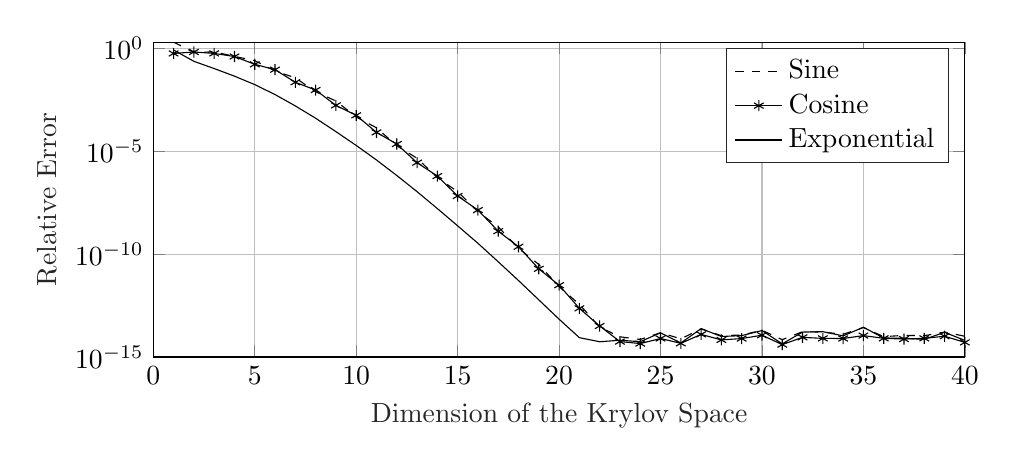
\begin{tikzpicture}

\begin{axis}[%
width=.85\linewidth,
height=4cm,
at={(0in,0in)},
scale only axis,
xmin=0,
xmax=40,
xlabel style={font=\color{white!15!black}},
xlabel={Dimension of the Krylov Space},
ymode=log,
ymin=1e-15,
ymax=1.97460071455281,
yminorticks=true,
ylabel style={font=\color{white!15!black}},
ylabel={Relative Error},
axis background/.style={fill=white},
xmajorgrids,
ymajorgrids,
yminorgrids,
legend style={legend cell align=left, align=left, draw=white!15!black}
]
\addplot [color=black, dashed]
  table[row sep=crcr]{%
1	1.97460071455281\\
2	0.619076115174164\\
3	0.660169549337596\\
4	0.399177784453014\\
5	0.247360478603165\\
6	0.0770623233479206\\
7	0.0361056649102699\\
8	0.00769698870977988\\
9	0.00271212764984173\\
10	0.000454664885646013\\
11	0.000135739008288232\\
12	1.82852337209858e-05\\
13	4.49914442853457e-06\\
14	5.17257496743468e-07\\
15	1.07880859681473e-07\\
16	1.14376479728179e-08\\
17	2.09273923908619e-09\\
18	1.91041894769733e-10\\
19	3.13086178596836e-11\\
20	2.60962651690699e-12\\
21	3.64703242223886e-13\\
22	2.81274242939596e-14\\
23	9.62733716238096e-15\\
24	7.11290334464613e-15\\
25	1.51875567025694e-14\\
26	7.67825133359383e-15\\
27	2.32013926946209e-14\\
28	1.09477870379481e-14\\
29	1.17084987936614e-14\\
30	1.99235352280141e-14\\
31	6.97756529550258e-15\\
32	1.70419495575996e-14\\
33	1.62365809662753e-14\\
34	1.28152537970561e-14\\
35	2.69179073371364e-14\\
36	9.78502038434061e-15\\
37	1.12829542277747e-14\\
38	1.08541889272337e-14\\
39	1.64152844940693e-14\\
40	1.01902790145147e-14\\
41	0\\
42	0\\
43	0\\
44	0\\
45	0\\
46	0\\
47	0\\
48	0\\
49	0\\
50	0\\
51	0\\
52	0\\
53	0\\
54	0\\
55	0\\
56	0\\
57	0\\
58	0\\
59	0\\
60	0\\
61	0\\
62	0\\
63	0\\
64	0\\
65	0\\
66	0\\
67	0\\
68	0\\
69	0\\
70	0\\
71	0\\
72	0\\
73	0\\
74	0\\
75	0\\
76	0\\
77	0\\
78	0\\
79	0\\
80	0\\
81	0\\
82	0\\
83	0\\
84	0\\
85	0\\
86	0\\
87	0\\
88	0\\
89	0\\
90	0\\
91	0\\
92	0\\
93	0\\
94	0\\
95	0\\
96	0\\
97	0\\
98	0\\
99	0\\
100	0\\
101	0\\
102	0\\
103	0\\
104	0\\
105	0\\
106	0\\
107	0\\
108	0\\
109	0\\
110	0\\
111	0\\
112	0\\
113	0\\
114	0\\
115	0\\
116	0\\
117	0\\
118	0\\
119	0\\
120	0\\
121	0\\
122	0\\
123	0\\
124	0\\
125	0\\
126	0\\
127	0\\
128	0\\
129	0\\
130	0\\
131	0\\
132	0\\
133	0\\
134	0\\
135	0\\
136	0\\
137	0\\
138	0\\
139	0\\
140	0\\
141	0\\
142	0\\
143	0\\
144	0\\
145	0\\
146	0\\
147	0\\
148	0\\
149	0\\
150	0\\
151	0\\
152	0\\
153	0\\
154	0\\
155	0\\
156	0\\
157	0\\
158	0\\
159	0\\
160	0\\
161	0\\
162	0\\
163	0\\
164	0\\
165	0\\
166	0\\
167	0\\
168	0\\
169	0\\
170	0\\
171	0\\
172	0\\
173	0\\
174	0\\
175	0\\
176	0\\
177	0\\
178	0\\
179	0\\
180	0\\
181	0\\
182	0\\
183	0\\
184	0\\
185	0\\
186	0\\
187	0\\
188	0\\
189	0\\
190	0\\
191	0\\
192	0\\
193	0\\
194	0\\
195	0\\
196	0\\
197	0\\
198	0\\
199	0\\
200	0\\
201	0\\
202	0\\
203	0\\
204	0\\
205	0\\
206	0\\
207	0\\
208	0\\
209	0\\
210	0\\
211	0\\
212	0\\
213	0\\
214	0\\
215	0\\
216	0\\
217	0\\
218	0\\
219	0\\
220	0\\
221	0\\
222	0\\
223	0\\
224	0\\
225	0\\
226	0\\
227	0\\
228	0\\
229	0\\
230	0\\
231	0\\
232	0\\
233	0\\
234	0\\
235	0\\
236	0\\
237	0\\
238	0\\
239	0\\
240	0\\
241	0\\
242	0\\
243	0\\
244	0\\
245	0\\
246	0\\
247	0\\
248	0\\
249	0\\
250	0\\
251	0\\
252	0\\
253	0\\
254	0\\
255	0\\
256	0\\
257	0\\
258	0\\
259	0\\
260	0\\
261	0\\
262	0\\
263	0\\
264	0\\
265	0\\
266	0\\
267	0\\
268	0\\
269	0\\
270	0\\
271	0\\
272	0\\
273	0\\
274	0\\
275	0\\
276	0\\
277	0\\
278	0\\
279	0\\
280	0\\
281	0\\
282	0\\
283	0\\
284	0\\
285	0\\
286	0\\
287	0\\
288	0\\
289	0\\
290	0\\
291	0\\
292	0\\
293	0\\
294	0\\
295	0\\
296	0\\
297	0\\
298	0\\
299	0\\
300	0\\
301	0\\
302	0\\
303	0\\
304	0\\
305	0\\
306	0\\
307	0\\
308	0\\
309	0\\
310	0\\
311	0\\
312	0\\
313	0\\
314	0\\
315	0\\
316	0\\
317	0\\
318	0\\
319	0\\
320	0\\
321	0\\
322	0\\
323	0\\
324	0\\
325	0\\
326	0\\
327	0\\
328	0\\
329	0\\
330	0\\
331	0\\
332	0\\
333	0\\
334	0\\
335	0\\
336	0\\
337	0\\
338	0\\
339	0\\
340	0\\
341	0\\
342	0\\
343	0\\
344	0\\
345	0\\
346	0\\
347	0\\
348	0\\
349	0\\
350	0\\
351	0\\
352	0\\
353	0\\
354	0\\
355	0\\
356	0\\
357	0\\
358	0\\
359	0\\
360	0\\
361	0\\
362	0\\
363	0\\
364	0\\
365	0\\
366	0\\
367	0\\
368	0\\
369	0\\
370	0\\
371	0\\
372	0\\
373	0\\
374	0\\
375	0\\
376	0\\
377	0\\
378	0\\
379	0\\
380	0\\
381	0\\
382	0\\
383	0\\
384	0\\
385	0\\
386	0\\
387	0\\
388	0\\
389	0\\
390	0\\
391	0\\
392	0\\
393	0\\
394	0\\
395	0\\
396	0\\
397	0\\
398	0\\
399	0\\
400	0\\
401	0\\
402	0\\
403	0\\
404	0\\
405	0\\
406	0\\
407	0\\
408	0\\
409	0\\
410	0\\
411	0\\
412	0\\
413	0\\
414	0\\
415	0\\
416	0\\
417	0\\
418	0\\
419	0\\
420	0\\
421	0\\
422	0\\
423	0\\
424	0\\
425	0\\
426	0\\
427	0\\
428	0\\
429	0\\
430	0\\
431	0\\
432	0\\
433	0\\
434	0\\
435	0\\
436	0\\
437	0\\
438	0\\
439	0\\
440	0\\
441	0\\
442	0\\
443	0\\
444	0\\
445	0\\
446	0\\
447	0\\
448	0\\
449	0\\
450	0\\
451	0\\
452	0\\
453	0\\
454	0\\
455	0\\
456	0\\
457	0\\
458	0\\
459	0\\
460	0\\
461	0\\
462	0\\
463	0\\
464	0\\
465	0\\
466	0\\
467	0\\
468	0\\
469	0\\
470	0\\
471	0\\
472	0\\
473	0\\
474	0\\
475	0\\
476	0\\
477	0\\
478	0\\
479	0\\
480	0\\
481	0\\
482	0\\
483	0\\
484	0\\
485	0\\
486	0\\
487	0\\
488	0\\
489	0\\
490	0\\
491	0\\
492	0\\
493	0\\
494	0\\
495	0\\
496	0\\
497	0\\
498	0\\
499	0\\
500	0\\
501	0\\
502	0\\
503	0\\
504	0\\
505	0\\
506	0\\
507	0\\
508	0\\
509	0\\
510	0\\
511	0\\
512	0\\
513	0\\
514	0\\
515	0\\
516	0\\
517	0\\
518	0\\
519	0\\
520	0\\
521	0\\
522	0\\
523	0\\
524	0\\
525	0\\
526	0\\
527	0\\
528	0\\
529	0\\
530	0\\
531	0\\
532	0\\
533	0\\
534	0\\
535	0\\
536	0\\
537	0\\
538	0\\
539	0\\
540	0\\
541	0\\
542	0\\
543	0\\
544	0\\
545	0\\
546	0\\
547	0\\
548	0\\
549	0\\
550	0\\
551	0\\
552	0\\
553	0\\
554	0\\
555	0\\
556	0\\
557	0\\
558	0\\
559	0\\
560	0\\
561	0\\
562	0\\
563	0\\
564	0\\
565	0\\
566	0\\
567	0\\
568	0\\
569	0\\
570	0\\
571	0\\
572	0\\
573	0\\
574	0\\
575	0\\
576	0\\
577	0\\
578	0\\
579	0\\
580	0\\
581	0\\
582	0\\
583	0\\
584	0\\
585	0\\
586	0\\
587	0\\
588	0\\
589	0\\
590	0\\
591	0\\
592	0\\
593	0\\
594	0\\
595	0\\
596	0\\
597	0\\
598	0\\
599	0\\
600	0\\
601	0\\
602	0\\
603	0\\
604	0\\
605	0\\
606	0\\
607	0\\
608	0\\
609	0\\
610	0\\
611	0\\
612	0\\
613	0\\
614	0\\
615	0\\
616	0\\
617	0\\
618	0\\
619	0\\
620	0\\
621	0\\
622	0\\
623	0\\
624	0\\
625	0\\
626	0\\
627	0\\
628	0\\
629	0\\
630	0\\
631	0\\
632	0\\
633	0\\
634	0\\
635	0\\
636	0\\
637	0\\
638	0\\
639	0\\
640	0\\
641	0\\
642	0\\
643	0\\
644	0\\
645	0\\
646	0\\
647	0\\
648	0\\
649	0\\
650	0\\
651	0\\
652	0\\
653	0\\
654	0\\
655	0\\
656	0\\
657	0\\
658	0\\
659	0\\
660	0\\
661	0\\
662	0\\
663	0\\
664	0\\
665	0\\
666	0\\
667	0\\
668	0\\
669	0\\
670	0\\
671	0\\
672	0\\
673	0\\
674	0\\
675	0\\
676	0\\
677	0\\
678	0\\
679	0\\
680	0\\
681	0\\
682	0\\
683	0\\
684	0\\
685	0\\
686	0\\
687	0\\
688	0\\
689	0\\
690	0\\
691	0\\
692	0\\
693	0\\
694	0\\
695	0\\
696	0\\
697	0\\
698	0\\
699	0\\
700	0\\
701	0\\
702	0\\
703	0\\
704	0\\
705	0\\
706	0\\
707	0\\
708	0\\
709	0\\
710	0\\
711	0\\
712	0\\
713	0\\
714	0\\
715	0\\
716	0\\
717	0\\
718	0\\
719	0\\
720	0\\
721	0\\
722	0\\
723	0\\
724	0\\
725	0\\
726	0\\
727	0\\
728	0\\
729	0\\
730	0\\
731	0\\
732	0\\
733	0\\
734	0\\
735	0\\
736	0\\
737	0\\
738	0\\
739	0\\
740	0\\
741	0\\
742	0\\
743	0\\
744	0\\
745	0\\
746	0\\
747	0\\
748	0\\
749	0\\
750	0\\
751	0\\
752	0\\
753	0\\
754	0\\
755	0\\
756	0\\
757	0\\
758	0\\
759	0\\
760	0\\
761	0\\
762	0\\
763	0\\
764	0\\
765	0\\
766	0\\
767	0\\
768	0\\
769	0\\
770	0\\
771	0\\
772	0\\
773	0\\
774	0\\
775	0\\
776	0\\
777	0\\
778	0\\
779	0\\
780	0\\
781	0\\
782	0\\
783	0\\
784	0\\
785	0\\
786	0\\
787	0\\
788	0\\
789	0\\
790	0\\
791	0\\
792	0\\
793	0\\
794	0\\
795	0\\
796	0\\
797	0\\
798	0\\
799	0\\
800	0\\
801	0\\
802	0\\
803	0\\
804	0\\
805	0\\
806	0\\
807	0\\
808	0\\
809	0\\
810	0\\
811	0\\
812	0\\
813	0\\
814	0\\
815	0\\
816	0\\
817	0\\
818	0\\
819	0\\
820	0\\
821	0\\
822	0\\
823	0\\
824	0\\
825	0\\
826	0\\
827	0\\
828	0\\
829	0\\
830	0\\
831	0\\
832	0\\
833	0\\
834	0\\
835	0\\
836	0\\
837	0\\
838	0\\
839	0\\
840	0\\
841	0\\
842	0\\
843	0\\
844	0\\
845	0\\
846	0\\
847	0\\
848	0\\
849	0\\
850	0\\
851	0\\
852	0\\
853	0\\
854	0\\
855	0\\
856	0\\
857	0\\
858	0\\
859	0\\
860	0\\
861	0\\
862	0\\
863	0\\
864	0\\
865	0\\
866	0\\
867	0\\
868	0\\
869	0\\
870	0\\
871	0\\
872	0\\
873	0\\
874	0\\
875	0\\
876	0\\
877	0\\
878	0\\
879	0\\
880	0\\
881	0\\
882	0\\
883	0\\
884	0\\
885	0\\
886	0\\
887	0\\
888	0\\
889	0\\
890	0\\
891	0\\
892	0\\
893	0\\
894	0\\
895	0\\
896	0\\
897	0\\
898	0\\
899	0\\
900	0\\
901	0\\
902	0\\
903	0\\
904	0\\
905	0\\
906	0\\
907	0\\
908	0\\
909	0\\
910	0\\
911	0\\
912	0\\
913	0\\
914	0\\
915	0\\
916	0\\
917	0\\
918	0\\
919	0\\
920	0\\
921	0\\
922	0\\
923	0\\
924	0\\
925	0\\
926	0\\
927	0\\
928	0\\
929	0\\
930	0\\
931	0\\
932	0\\
933	0\\
934	0\\
935	0\\
936	0\\
937	0\\
938	0\\
939	0\\
940	0\\
941	0\\
942	0\\
943	0\\
944	0\\
945	0\\
946	0\\
947	0\\
948	0\\
949	0\\
950	0\\
951	0\\
952	0\\
953	0\\
954	0\\
955	0\\
956	0\\
957	0\\
958	0\\
959	0\\
960	0\\
961	0\\
962	0\\
963	0\\
964	0\\
965	0\\
966	0\\
967	0\\
968	0\\
969	0\\
970	0\\
971	0\\
972	0\\
973	0\\
974	0\\
975	0\\
976	0\\
977	0\\
978	0\\
979	0\\
980	0\\
981	0\\
982	0\\
983	0\\
984	0\\
985	0\\
986	0\\
987	0\\
988	0\\
989	0\\
990	0\\
991	0\\
992	0\\
993	0\\
994	0\\
995	0\\
996	0\\
997	0\\
998	0\\
999	0\\
1000	0\\
1001	0\\
1002	0\\
1003	0\\
1004	0\\
1005	0\\
1006	0\\
1007	0\\
1008	0\\
1009	0\\
};
\addlegendentry{Sine}

\addplot [color=black, mark=asterisk, mark options={solid, black}]
  table[row sep=crcr]{%
1	0.553022669474569\\
2	0.652500810441648\\
3	0.556845817887251\\
4	0.393146704717499\\
5	0.163911995710726\\
6	0.0902214334096444\\
7	0.0220056909143109\\
8	0.00925746314021299\\
9	0.00166598892415074\\
10	0.000547989274983716\\
11	8.11973206825985e-05\\
12	2.21611524092059e-05\\
13	2.74095219712664e-06\\
14	6.1565013295927e-07\\
15	6.63480338780706e-08\\
16	1.37230704725437e-08\\
17	1.29386047360475e-09\\
18	2.27182562190856e-10\\
19	1.9212694183763e-11\\
20	3.09225915515234e-12\\
21	2.3169721460413e-13\\
22	3.21542765086078e-14\\
23	5.64166778839452e-15\\
24	4.51434115074838e-15\\
25	7.93413020012027e-15\\
26	4.6391922283268e-15\\
27	1.2576270609606e-14\\
28	6.77902898353538e-15\\
29	7.89884432562526e-15\\
30	1.14822488228154e-14\\
31	4.0177683495859e-15\\
32	9.04186080970131e-15\\
33	8.05544506510754e-15\\
34	7.95266318162819e-15\\
35	1.10013943938327e-14\\
36	8.1040004251156e-15\\
37	7.48412710445178e-15\\
38	8.09484948647143e-15\\
39	1.02384935377778e-14\\
40	5.14384998439096e-15\\
41	0\\
42	0\\
43	0\\
44	0\\
45	0\\
46	0\\
47	0\\
48	0\\
49	0\\
50	0\\
51	0\\
52	0\\
53	0\\
54	0\\
55	0\\
56	0\\
57	0\\
58	0\\
59	0\\
60	0\\
61	0\\
62	0\\
63	0\\
64	0\\
65	0\\
66	0\\
67	0\\
68	0\\
69	0\\
70	0\\
71	0\\
72	0\\
73	0\\
74	0\\
75	0\\
76	0\\
77	0\\
78	0\\
79	0\\
80	0\\
81	0\\
82	0\\
83	0\\
84	0\\
85	0\\
86	0\\
87	0\\
88	0\\
89	0\\
90	0\\
91	0\\
92	0\\
93	0\\
94	0\\
95	0\\
96	0\\
97	0\\
98	0\\
99	0\\
100	0\\
101	0\\
102	0\\
103	0\\
104	0\\
105	0\\
106	0\\
107	0\\
108	0\\
109	0\\
110	0\\
111	0\\
112	0\\
113	0\\
114	0\\
115	0\\
116	0\\
117	0\\
118	0\\
119	0\\
120	0\\
121	0\\
122	0\\
123	0\\
124	0\\
125	0\\
126	0\\
127	0\\
128	0\\
129	0\\
130	0\\
131	0\\
132	0\\
133	0\\
134	0\\
135	0\\
136	0\\
137	0\\
138	0\\
139	0\\
140	0\\
141	0\\
142	0\\
143	0\\
144	0\\
145	0\\
146	0\\
147	0\\
148	0\\
149	0\\
150	0\\
151	0\\
152	0\\
153	0\\
154	0\\
155	0\\
156	0\\
157	0\\
158	0\\
159	0\\
160	0\\
161	0\\
162	0\\
163	0\\
164	0\\
165	0\\
166	0\\
167	0\\
168	0\\
169	0\\
170	0\\
171	0\\
172	0\\
173	0\\
174	0\\
175	0\\
176	0\\
177	0\\
178	0\\
179	0\\
180	0\\
181	0\\
182	0\\
183	0\\
184	0\\
185	0\\
186	0\\
187	0\\
188	0\\
189	0\\
190	0\\
191	0\\
192	0\\
193	0\\
194	0\\
195	0\\
196	0\\
197	0\\
198	0\\
199	0\\
200	0\\
201	0\\
202	0\\
203	0\\
204	0\\
205	0\\
206	0\\
207	0\\
208	0\\
209	0\\
210	0\\
211	0\\
212	0\\
213	0\\
214	0\\
215	0\\
216	0\\
217	0\\
218	0\\
219	0\\
220	0\\
221	0\\
222	0\\
223	0\\
224	0\\
225	0\\
226	0\\
227	0\\
228	0\\
229	0\\
230	0\\
231	0\\
232	0\\
233	0\\
234	0\\
235	0\\
236	0\\
237	0\\
238	0\\
239	0\\
240	0\\
241	0\\
242	0\\
243	0\\
244	0\\
245	0\\
246	0\\
247	0\\
248	0\\
249	0\\
250	0\\
251	0\\
252	0\\
253	0\\
254	0\\
255	0\\
256	0\\
257	0\\
258	0\\
259	0\\
260	0\\
261	0\\
262	0\\
263	0\\
264	0\\
265	0\\
266	0\\
267	0\\
268	0\\
269	0\\
270	0\\
271	0\\
272	0\\
273	0\\
274	0\\
275	0\\
276	0\\
277	0\\
278	0\\
279	0\\
280	0\\
281	0\\
282	0\\
283	0\\
284	0\\
285	0\\
286	0\\
287	0\\
288	0\\
289	0\\
290	0\\
291	0\\
292	0\\
293	0\\
294	0\\
295	0\\
296	0\\
297	0\\
298	0\\
299	0\\
300	0\\
301	0\\
302	0\\
303	0\\
304	0\\
305	0\\
306	0\\
307	0\\
308	0\\
309	0\\
310	0\\
311	0\\
312	0\\
313	0\\
314	0\\
315	0\\
316	0\\
317	0\\
318	0\\
319	0\\
320	0\\
321	0\\
322	0\\
323	0\\
324	0\\
325	0\\
326	0\\
327	0\\
328	0\\
329	0\\
330	0\\
331	0\\
332	0\\
333	0\\
334	0\\
335	0\\
336	0\\
337	0\\
338	0\\
339	0\\
340	0\\
341	0\\
342	0\\
343	0\\
344	0\\
345	0\\
346	0\\
347	0\\
348	0\\
349	0\\
350	0\\
351	0\\
352	0\\
353	0\\
354	0\\
355	0\\
356	0\\
357	0\\
358	0\\
359	0\\
360	0\\
361	0\\
362	0\\
363	0\\
364	0\\
365	0\\
366	0\\
367	0\\
368	0\\
369	0\\
370	0\\
371	0\\
372	0\\
373	0\\
374	0\\
375	0\\
376	0\\
377	0\\
378	0\\
379	0\\
380	0\\
381	0\\
382	0\\
383	0\\
384	0\\
385	0\\
386	0\\
387	0\\
388	0\\
389	0\\
390	0\\
391	0\\
392	0\\
393	0\\
394	0\\
395	0\\
396	0\\
397	0\\
398	0\\
399	0\\
400	0\\
401	0\\
402	0\\
403	0\\
404	0\\
405	0\\
406	0\\
407	0\\
408	0\\
409	0\\
410	0\\
411	0\\
412	0\\
413	0\\
414	0\\
415	0\\
416	0\\
417	0\\
418	0\\
419	0\\
420	0\\
421	0\\
422	0\\
423	0\\
424	0\\
425	0\\
426	0\\
427	0\\
428	0\\
429	0\\
430	0\\
431	0\\
432	0\\
433	0\\
434	0\\
435	0\\
436	0\\
437	0\\
438	0\\
439	0\\
440	0\\
441	0\\
442	0\\
443	0\\
444	0\\
445	0\\
446	0\\
447	0\\
448	0\\
449	0\\
450	0\\
451	0\\
452	0\\
453	0\\
454	0\\
455	0\\
456	0\\
457	0\\
458	0\\
459	0\\
460	0\\
461	0\\
462	0\\
463	0\\
464	0\\
465	0\\
466	0\\
467	0\\
468	0\\
469	0\\
470	0\\
471	0\\
472	0\\
473	0\\
474	0\\
475	0\\
476	0\\
477	0\\
478	0\\
479	0\\
480	0\\
481	0\\
482	0\\
483	0\\
484	0\\
485	0\\
486	0\\
487	0\\
488	0\\
489	0\\
490	0\\
491	0\\
492	0\\
493	0\\
494	0\\
495	0\\
496	0\\
497	0\\
498	0\\
499	0\\
500	0\\
501	0\\
502	0\\
503	0\\
504	0\\
505	0\\
506	0\\
507	0\\
508	0\\
509	0\\
510	0\\
511	0\\
512	0\\
513	0\\
514	0\\
515	0\\
516	0\\
517	0\\
518	0\\
519	0\\
520	0\\
521	0\\
522	0\\
523	0\\
524	0\\
525	0\\
526	0\\
527	0\\
528	0\\
529	0\\
530	0\\
531	0\\
532	0\\
533	0\\
534	0\\
535	0\\
536	0\\
537	0\\
538	0\\
539	0\\
540	0\\
541	0\\
542	0\\
543	0\\
544	0\\
545	0\\
546	0\\
547	0\\
548	0\\
549	0\\
550	0\\
551	0\\
552	0\\
553	0\\
554	0\\
555	0\\
556	0\\
557	0\\
558	0\\
559	0\\
560	0\\
561	0\\
562	0\\
563	0\\
564	0\\
565	0\\
566	0\\
567	0\\
568	0\\
569	0\\
570	0\\
571	0\\
572	0\\
573	0\\
574	0\\
575	0\\
576	0\\
577	0\\
578	0\\
579	0\\
580	0\\
581	0\\
582	0\\
583	0\\
584	0\\
585	0\\
586	0\\
587	0\\
588	0\\
589	0\\
590	0\\
591	0\\
592	0\\
593	0\\
594	0\\
595	0\\
596	0\\
597	0\\
598	0\\
599	0\\
600	0\\
601	0\\
602	0\\
603	0\\
604	0\\
605	0\\
606	0\\
607	0\\
608	0\\
609	0\\
610	0\\
611	0\\
612	0\\
613	0\\
614	0\\
615	0\\
616	0\\
617	0\\
618	0\\
619	0\\
620	0\\
621	0\\
622	0\\
623	0\\
624	0\\
625	0\\
626	0\\
627	0\\
628	0\\
629	0\\
630	0\\
631	0\\
632	0\\
633	0\\
634	0\\
635	0\\
636	0\\
637	0\\
638	0\\
639	0\\
640	0\\
641	0\\
642	0\\
643	0\\
644	0\\
645	0\\
646	0\\
647	0\\
648	0\\
649	0\\
650	0\\
651	0\\
652	0\\
653	0\\
654	0\\
655	0\\
656	0\\
657	0\\
658	0\\
659	0\\
660	0\\
661	0\\
662	0\\
663	0\\
664	0\\
665	0\\
666	0\\
667	0\\
668	0\\
669	0\\
670	0\\
671	0\\
672	0\\
673	0\\
674	0\\
675	0\\
676	0\\
677	0\\
678	0\\
679	0\\
680	0\\
681	0\\
682	0\\
683	0\\
684	0\\
685	0\\
686	0\\
687	0\\
688	0\\
689	0\\
690	0\\
691	0\\
692	0\\
693	0\\
694	0\\
695	0\\
696	0\\
697	0\\
698	0\\
699	0\\
700	0\\
701	0\\
702	0\\
703	0\\
704	0\\
705	0\\
706	0\\
707	0\\
708	0\\
709	0\\
710	0\\
711	0\\
712	0\\
713	0\\
714	0\\
715	0\\
716	0\\
717	0\\
718	0\\
719	0\\
720	0\\
721	0\\
722	0\\
723	0\\
724	0\\
725	0\\
726	0\\
727	0\\
728	0\\
729	0\\
730	0\\
731	0\\
732	0\\
733	0\\
734	0\\
735	0\\
736	0\\
737	0\\
738	0\\
739	0\\
740	0\\
741	0\\
742	0\\
743	0\\
744	0\\
745	0\\
746	0\\
747	0\\
748	0\\
749	0\\
750	0\\
751	0\\
752	0\\
753	0\\
754	0\\
755	0\\
756	0\\
757	0\\
758	0\\
759	0\\
760	0\\
761	0\\
762	0\\
763	0\\
764	0\\
765	0\\
766	0\\
767	0\\
768	0\\
769	0\\
770	0\\
771	0\\
772	0\\
773	0\\
774	0\\
775	0\\
776	0\\
777	0\\
778	0\\
779	0\\
780	0\\
781	0\\
782	0\\
783	0\\
784	0\\
785	0\\
786	0\\
787	0\\
788	0\\
789	0\\
790	0\\
791	0\\
792	0\\
793	0\\
794	0\\
795	0\\
796	0\\
797	0\\
798	0\\
799	0\\
800	0\\
801	0\\
802	0\\
803	0\\
804	0\\
805	0\\
806	0\\
807	0\\
808	0\\
809	0\\
810	0\\
811	0\\
812	0\\
813	0\\
814	0\\
815	0\\
816	0\\
817	0\\
818	0\\
819	0\\
820	0\\
821	0\\
822	0\\
823	0\\
824	0\\
825	0\\
826	0\\
827	0\\
828	0\\
829	0\\
830	0\\
831	0\\
832	0\\
833	0\\
834	0\\
835	0\\
836	0\\
837	0\\
838	0\\
839	0\\
840	0\\
841	0\\
842	0\\
843	0\\
844	0\\
845	0\\
846	0\\
847	0\\
848	0\\
849	0\\
850	0\\
851	0\\
852	0\\
853	0\\
854	0\\
855	0\\
856	0\\
857	0\\
858	0\\
859	0\\
860	0\\
861	0\\
862	0\\
863	0\\
864	0\\
865	0\\
866	0\\
867	0\\
868	0\\
869	0\\
870	0\\
871	0\\
872	0\\
873	0\\
874	0\\
875	0\\
876	0\\
877	0\\
878	0\\
879	0\\
880	0\\
881	0\\
882	0\\
883	0\\
884	0\\
885	0\\
886	0\\
887	0\\
888	0\\
889	0\\
890	0\\
891	0\\
892	0\\
893	0\\
894	0\\
895	0\\
896	0\\
897	0\\
898	0\\
899	0\\
900	0\\
901	0\\
902	0\\
903	0\\
904	0\\
905	0\\
906	0\\
907	0\\
908	0\\
909	0\\
910	0\\
911	0\\
912	0\\
913	0\\
914	0\\
915	0\\
916	0\\
917	0\\
918	0\\
919	0\\
920	0\\
921	0\\
922	0\\
923	0\\
924	0\\
925	0\\
926	0\\
927	0\\
928	0\\
929	0\\
930	0\\
931	0\\
932	0\\
933	0\\
934	0\\
935	0\\
936	0\\
937	0\\
938	0\\
939	0\\
940	0\\
941	0\\
942	0\\
943	0\\
944	0\\
945	0\\
946	0\\
947	0\\
948	0\\
949	0\\
950	0\\
951	0\\
952	0\\
953	0\\
954	0\\
955	0\\
956	0\\
957	0\\
958	0\\
959	0\\
960	0\\
961	0\\
962	0\\
963	0\\
964	0\\
965	0\\
966	0\\
967	0\\
968	0\\
969	0\\
970	0\\
971	0\\
972	0\\
973	0\\
974	0\\
975	0\\
976	0\\
977	0\\
978	0\\
979	0\\
980	0\\
981	0\\
982	0\\
983	0\\
984	0\\
985	0\\
986	0\\
987	0\\
988	0\\
989	0\\
990	0\\
991	0\\
992	0\\
993	0\\
994	0\\
995	0\\
996	0\\
997	0\\
998	0\\
999	0\\
1000	0\\
1001	0\\
1002	0\\
1003	0\\
1004	0\\
1005	0\\
1006	0\\
1007	0\\
1008	0\\
1009	0\\
};
\addlegendentry{Cosine}

\addplot [color=black]
  table[row sep=crcr]{%
1	0.810160768398566\\
2	0.229597555066745\\
3	0.102290316758195\\
4	0.0437046653904947\\
5	0.0169804751902121\\
6	0.00557496262586476\\
7	0.00156595100800799\\
8	0.000396056478432868\\
9	8.84303753275448e-05\\
10	1.89088960206794e-05\\
11	3.71575067543707e-06\\
12	6.56134609907737e-07\\
13	1.07576636566187e-07\\
14	1.62438015616103e-08\\
15	2.3528094725792e-09\\
16	3.34590486347729e-10\\
17	4.23306707802162e-11\\
18	5.18077197818621e-12\\
19	5.9845251358946e-13\\
20	6.87987864459691e-14\\
21	8.73417994770503e-15\\
22	5.52804739741531e-15\\
23	6.53401651082081e-15\\
24	5.56678162119376e-15\\
25	1.50402937528157e-14\\
26	4.79403144899064e-15\\
27	2.40530543307074e-14\\
28	9.95338419206409e-15\\
29	1.09512178811563e-14\\
30	1.94131024469222e-14\\
31	4.36210616339599e-15\\
32	1.63074867240445e-14\\
33	1.70529970192069e-14\\
34	1.06615066767856e-14\\
35	2.79779086645277e-14\\
36	8.43941494774915e-15\\
37	8.12168270938859e-15\\
38	7.22256454077389e-15\\
39	1.58931716898493e-14\\
40	6.42117779932584e-15\\
41	0\\
42	0\\
43	0\\
44	0\\
45	0\\
46	0\\
47	0\\
48	0\\
49	0\\
50	0\\
51	0\\
52	0\\
53	0\\
54	0\\
55	0\\
56	0\\
57	0\\
58	0\\
59	0\\
60	0\\
61	0\\
62	0\\
63	0\\
64	0\\
65	0\\
66	0\\
67	0\\
68	0\\
69	0\\
70	0\\
71	0\\
72	0\\
73	0\\
74	0\\
75	0\\
76	0\\
77	0\\
78	0\\
79	0\\
80	0\\
81	0\\
82	0\\
83	0\\
84	0\\
85	0\\
86	0\\
87	0\\
88	0\\
89	0\\
90	0\\
91	0\\
92	0\\
93	0\\
94	0\\
95	0\\
96	0\\
97	0\\
98	0\\
99	0\\
100	0\\
101	0\\
102	0\\
103	0\\
104	0\\
105	0\\
106	0\\
107	0\\
108	0\\
109	0\\
110	0\\
111	0\\
112	0\\
113	0\\
114	0\\
115	0\\
116	0\\
117	0\\
118	0\\
119	0\\
120	0\\
121	0\\
122	0\\
123	0\\
124	0\\
125	0\\
126	0\\
127	0\\
128	0\\
129	0\\
130	0\\
131	0\\
132	0\\
133	0\\
134	0\\
135	0\\
136	0\\
137	0\\
138	0\\
139	0\\
140	0\\
141	0\\
142	0\\
143	0\\
144	0\\
145	0\\
146	0\\
147	0\\
148	0\\
149	0\\
150	0\\
151	0\\
152	0\\
153	0\\
154	0\\
155	0\\
156	0\\
157	0\\
158	0\\
159	0\\
160	0\\
161	0\\
162	0\\
163	0\\
164	0\\
165	0\\
166	0\\
167	0\\
168	0\\
169	0\\
170	0\\
171	0\\
172	0\\
173	0\\
174	0\\
175	0\\
176	0\\
177	0\\
178	0\\
179	0\\
180	0\\
181	0\\
182	0\\
183	0\\
184	0\\
185	0\\
186	0\\
187	0\\
188	0\\
189	0\\
190	0\\
191	0\\
192	0\\
193	0\\
194	0\\
195	0\\
196	0\\
197	0\\
198	0\\
199	0\\
200	0\\
201	0\\
202	0\\
203	0\\
204	0\\
205	0\\
206	0\\
207	0\\
208	0\\
209	0\\
210	0\\
211	0\\
212	0\\
213	0\\
214	0\\
215	0\\
216	0\\
217	0\\
218	0\\
219	0\\
220	0\\
221	0\\
222	0\\
223	0\\
224	0\\
225	0\\
226	0\\
227	0\\
228	0\\
229	0\\
230	0\\
231	0\\
232	0\\
233	0\\
234	0\\
235	0\\
236	0\\
237	0\\
238	0\\
239	0\\
240	0\\
241	0\\
242	0\\
243	0\\
244	0\\
245	0\\
246	0\\
247	0\\
248	0\\
249	0\\
250	0\\
251	0\\
252	0\\
253	0\\
254	0\\
255	0\\
256	0\\
257	0\\
258	0\\
259	0\\
260	0\\
261	0\\
262	0\\
263	0\\
264	0\\
265	0\\
266	0\\
267	0\\
268	0\\
269	0\\
270	0\\
271	0\\
272	0\\
273	0\\
274	0\\
275	0\\
276	0\\
277	0\\
278	0\\
279	0\\
280	0\\
281	0\\
282	0\\
283	0\\
284	0\\
285	0\\
286	0\\
287	0\\
288	0\\
289	0\\
290	0\\
291	0\\
292	0\\
293	0\\
294	0\\
295	0\\
296	0\\
297	0\\
298	0\\
299	0\\
300	0\\
301	0\\
302	0\\
303	0\\
304	0\\
305	0\\
306	0\\
307	0\\
308	0\\
309	0\\
310	0\\
311	0\\
312	0\\
313	0\\
314	0\\
315	0\\
316	0\\
317	0\\
318	0\\
319	0\\
320	0\\
321	0\\
322	0\\
323	0\\
324	0\\
325	0\\
326	0\\
327	0\\
328	0\\
329	0\\
330	0\\
331	0\\
332	0\\
333	0\\
334	0\\
335	0\\
336	0\\
337	0\\
338	0\\
339	0\\
340	0\\
341	0\\
342	0\\
343	0\\
344	0\\
345	0\\
346	0\\
347	0\\
348	0\\
349	0\\
350	0\\
351	0\\
352	0\\
353	0\\
354	0\\
355	0\\
356	0\\
357	0\\
358	0\\
359	0\\
360	0\\
361	0\\
362	0\\
363	0\\
364	0\\
365	0\\
366	0\\
367	0\\
368	0\\
369	0\\
370	0\\
371	0\\
372	0\\
373	0\\
374	0\\
375	0\\
376	0\\
377	0\\
378	0\\
379	0\\
380	0\\
381	0\\
382	0\\
383	0\\
384	0\\
385	0\\
386	0\\
387	0\\
388	0\\
389	0\\
390	0\\
391	0\\
392	0\\
393	0\\
394	0\\
395	0\\
396	0\\
397	0\\
398	0\\
399	0\\
400	0\\
401	0\\
402	0\\
403	0\\
404	0\\
405	0\\
406	0\\
407	0\\
408	0\\
409	0\\
410	0\\
411	0\\
412	0\\
413	0\\
414	0\\
415	0\\
416	0\\
417	0\\
418	0\\
419	0\\
420	0\\
421	0\\
422	0\\
423	0\\
424	0\\
425	0\\
426	0\\
427	0\\
428	0\\
429	0\\
430	0\\
431	0\\
432	0\\
433	0\\
434	0\\
435	0\\
436	0\\
437	0\\
438	0\\
439	0\\
440	0\\
441	0\\
442	0\\
443	0\\
444	0\\
445	0\\
446	0\\
447	0\\
448	0\\
449	0\\
450	0\\
451	0\\
452	0\\
453	0\\
454	0\\
455	0\\
456	0\\
457	0\\
458	0\\
459	0\\
460	0\\
461	0\\
462	0\\
463	0\\
464	0\\
465	0\\
466	0\\
467	0\\
468	0\\
469	0\\
470	0\\
471	0\\
472	0\\
473	0\\
474	0\\
475	0\\
476	0\\
477	0\\
478	0\\
479	0\\
480	0\\
481	0\\
482	0\\
483	0\\
484	0\\
485	0\\
486	0\\
487	0\\
488	0\\
489	0\\
490	0\\
491	0\\
492	0\\
493	0\\
494	0\\
495	0\\
496	0\\
497	0\\
498	0\\
499	0\\
500	0\\
501	0\\
502	0\\
503	0\\
504	0\\
505	0\\
506	0\\
507	0\\
508	0\\
509	0\\
510	0\\
511	0\\
512	0\\
513	0\\
514	0\\
515	0\\
516	0\\
517	0\\
518	0\\
519	0\\
520	0\\
521	0\\
522	0\\
523	0\\
524	0\\
525	0\\
526	0\\
527	0\\
528	0\\
529	0\\
530	0\\
531	0\\
532	0\\
533	0\\
534	0\\
535	0\\
536	0\\
537	0\\
538	0\\
539	0\\
540	0\\
541	0\\
542	0\\
543	0\\
544	0\\
545	0\\
546	0\\
547	0\\
548	0\\
549	0\\
550	0\\
551	0\\
552	0\\
553	0\\
554	0\\
555	0\\
556	0\\
557	0\\
558	0\\
559	0\\
560	0\\
561	0\\
562	0\\
563	0\\
564	0\\
565	0\\
566	0\\
567	0\\
568	0\\
569	0\\
570	0\\
571	0\\
572	0\\
573	0\\
574	0\\
575	0\\
576	0\\
577	0\\
578	0\\
579	0\\
580	0\\
581	0\\
582	0\\
583	0\\
584	0\\
585	0\\
586	0\\
587	0\\
588	0\\
589	0\\
590	0\\
591	0\\
592	0\\
593	0\\
594	0\\
595	0\\
596	0\\
597	0\\
598	0\\
599	0\\
600	0\\
601	0\\
602	0\\
603	0\\
604	0\\
605	0\\
606	0\\
607	0\\
608	0\\
609	0\\
610	0\\
611	0\\
612	0\\
613	0\\
614	0\\
615	0\\
616	0\\
617	0\\
618	0\\
619	0\\
620	0\\
621	0\\
622	0\\
623	0\\
624	0\\
625	0\\
626	0\\
627	0\\
628	0\\
629	0\\
630	0\\
631	0\\
632	0\\
633	0\\
634	0\\
635	0\\
636	0\\
637	0\\
638	0\\
639	0\\
640	0\\
641	0\\
642	0\\
643	0\\
644	0\\
645	0\\
646	0\\
647	0\\
648	0\\
649	0\\
650	0\\
651	0\\
652	0\\
653	0\\
654	0\\
655	0\\
656	0\\
657	0\\
658	0\\
659	0\\
660	0\\
661	0\\
662	0\\
663	0\\
664	0\\
665	0\\
666	0\\
667	0\\
668	0\\
669	0\\
670	0\\
671	0\\
672	0\\
673	0\\
674	0\\
675	0\\
676	0\\
677	0\\
678	0\\
679	0\\
680	0\\
681	0\\
682	0\\
683	0\\
684	0\\
685	0\\
686	0\\
687	0\\
688	0\\
689	0\\
690	0\\
691	0\\
692	0\\
693	0\\
694	0\\
695	0\\
696	0\\
697	0\\
698	0\\
699	0\\
700	0\\
701	0\\
702	0\\
703	0\\
704	0\\
705	0\\
706	0\\
707	0\\
708	0\\
709	0\\
710	0\\
711	0\\
712	0\\
713	0\\
714	0\\
715	0\\
716	0\\
717	0\\
718	0\\
719	0\\
720	0\\
721	0\\
722	0\\
723	0\\
724	0\\
725	0\\
726	0\\
727	0\\
728	0\\
729	0\\
730	0\\
731	0\\
732	0\\
733	0\\
734	0\\
735	0\\
736	0\\
737	0\\
738	0\\
739	0\\
740	0\\
741	0\\
742	0\\
743	0\\
744	0\\
745	0\\
746	0\\
747	0\\
748	0\\
749	0\\
750	0\\
751	0\\
752	0\\
753	0\\
754	0\\
755	0\\
756	0\\
757	0\\
758	0\\
759	0\\
760	0\\
761	0\\
762	0\\
763	0\\
764	0\\
765	0\\
766	0\\
767	0\\
768	0\\
769	0\\
770	0\\
771	0\\
772	0\\
773	0\\
774	0\\
775	0\\
776	0\\
777	0\\
778	0\\
779	0\\
780	0\\
781	0\\
782	0\\
783	0\\
784	0\\
785	0\\
786	0\\
787	0\\
788	0\\
789	0\\
790	0\\
791	0\\
792	0\\
793	0\\
794	0\\
795	0\\
796	0\\
797	0\\
798	0\\
799	0\\
800	0\\
801	0\\
802	0\\
803	0\\
804	0\\
805	0\\
806	0\\
807	0\\
808	0\\
809	0\\
810	0\\
811	0\\
812	0\\
813	0\\
814	0\\
815	0\\
816	0\\
817	0\\
818	0\\
819	0\\
820	0\\
821	0\\
822	0\\
823	0\\
824	0\\
825	0\\
826	0\\
827	0\\
828	0\\
829	0\\
830	0\\
831	0\\
832	0\\
833	0\\
834	0\\
835	0\\
836	0\\
837	0\\
838	0\\
839	0\\
840	0\\
841	0\\
842	0\\
843	0\\
844	0\\
845	0\\
846	0\\
847	0\\
848	0\\
849	0\\
850	0\\
851	0\\
852	0\\
853	0\\
854	0\\
855	0\\
856	0\\
857	0\\
858	0\\
859	0\\
860	0\\
861	0\\
862	0\\
863	0\\
864	0\\
865	0\\
866	0\\
867	0\\
868	0\\
869	0\\
870	0\\
871	0\\
872	0\\
873	0\\
874	0\\
875	0\\
876	0\\
877	0\\
878	0\\
879	0\\
880	0\\
881	0\\
882	0\\
883	0\\
884	0\\
885	0\\
886	0\\
887	0\\
888	0\\
889	0\\
890	0\\
891	0\\
892	0\\
893	0\\
894	0\\
895	0\\
896	0\\
897	0\\
898	0\\
899	0\\
900	0\\
901	0\\
902	0\\
903	0\\
904	0\\
905	0\\
906	0\\
907	0\\
908	0\\
909	0\\
910	0\\
911	0\\
912	0\\
913	0\\
914	0\\
915	0\\
916	0\\
917	0\\
918	0\\
919	0\\
920	0\\
921	0\\
922	0\\
923	0\\
924	0\\
925	0\\
926	0\\
927	0\\
928	0\\
929	0\\
930	0\\
931	0\\
932	0\\
933	0\\
934	0\\
935	0\\
936	0\\
937	0\\
938	0\\
939	0\\
940	0\\
941	0\\
942	0\\
943	0\\
944	0\\
945	0\\
946	0\\
947	0\\
948	0\\
949	0\\
950	0\\
951	0\\
952	0\\
953	0\\
954	0\\
955	0\\
956	0\\
957	0\\
958	0\\
959	0\\
960	0\\
961	0\\
962	0\\
963	0\\
964	0\\
965	0\\
966	0\\
967	0\\
968	0\\
969	0\\
970	0\\
971	0\\
972	0\\
973	0\\
974	0\\
975	0\\
976	0\\
977	0\\
978	0\\
979	0\\
980	0\\
981	0\\
982	0\\
983	0\\
984	0\\
985	0\\
986	0\\
987	0\\
988	0\\
989	0\\
990	0\\
991	0\\
992	0\\
993	0\\
994	0\\
995	0\\
996	0\\
997	0\\
998	0\\
999	0\\
1000	0\\
1001	0\\
1002	0\\
1003	0\\
1004	0\\
1005	0\\
1006	0\\
1007	0\\
1008	0\\
1009	0\\
};
\addlegendentry{Exponential}

\end{axis}
\end{tikzpicture}%
        \caption{}
        \label{fig:comp_fab_assignement}
    \end{subfigure}
    \caption{Evaluation of the performance of the matrix-vector product routine. We compare the performance of our method against the naive way of doing it in \texttt{Matlab}. We test it on three different functions : Sine (- -), Cosine (-*) and Exponenial (--) on figure (b). Those functions are applied to a large matrix $\mathbf{A}$ with sparisity pattern given in (a). Our method allows for precise approximation of $f(\mathbf{A})b$ even when working on a very low rank Hessenberg reduction (b). The vector $\mathbf{b}$ is a random vector whose coefficients are uniformly distributed such that $b_i\sim\mathcal{U}(0,1)$.}
    \label{fig:comp_fab}
\end{figure}

Obviously, this very interesting result lets us think that there is a lot of potential computational gain in evaluating $f(\mathbf{A})\mathbf{b}$ on this smaller Krylov subspace. The computational gain for the problem solved in figure \ref{fig:comp_fab} is described in Table \ref{tab:fab}. We note that for this problem, our method considerably outperforms the naive approach of evaluating $f(\mathbf{A})$ seperately, regardless of the function (though the biggest gain seem to come from the matrix exponential). 

However, this does not give us any insight about how those two algorithms sacle up or down. To investigate this, we will use the BCSPWR matrix collection. This collection contains matrices of different sizes, and different sparsity patterns. We will test our method against the naive approach on this collection. The results are depicted in Table \ref{tab:fab2}. We notice that for very low dimension ($n < 300$) the naive approach slightly outperforms ours for trigonometric functions. However, for larger matrices, and for the exponential function, working in the Kryloc subspace is the way to go. For the largest matrix, where $n=5300$, the naive approach takes half a minute, while our method takes less than a tenth of a second. This is a considerable gain in performance, and could be crucial in some applications. As this margin increases with the matrix size, we can expect our method to be even more efficient for larger matrices. One final interesting note, is that the optimal Krylov space dimension does not change much with the matrix size. This is a very interesting result, as it means that we can expect our method to be efficient for a wide range of matrix sizes, and explains why it does not suffer from scaling up ($f(\mathbf{H_k})$, which is the costly operation, is somewhat the same size whatever the tested matrix).

\begin{table}
    \centering
    \caption{Comparison of computational performance of both methods for evaluating $f(\mathbf{A}\mathbf{b})$ with $\mathbf{A}$ the matrix in \ref{fig:comp_fab_pattern}. Performance was measured in ms. Optimal $k$ was determined when the relative error went below $1e-14$, as we worked on double precision. Tests were run on an Intel Core i7-1185G7 @ 3.00GHz with 16GB RAM. We note that for this problem, our method is outperforming by a significant margin the naive approach.}
    \begin{tabular}{|c|c|c|c|}
        \hline
        \textbf{fun} & \textbf{Naive way (ms)} & \textbf{Krylov method (ms)} & \textbf{Optimal $k$} \\\hline
        \texttt{exp()} & 151.2 & 6.3 & 21 \\ \hline
        \texttt{cos()} & 121.8 & 11.2 & 23 \\ \hline
        \texttt{sin()} & 112.6 & 8.1 & 23 \\
        \hline
    \end{tabular}
    \label{tab:fab}
\end{table}

\begin{table}
    \centering
    \caption{Comparison of the naive approach and the Krylov approach on BCSPWR matrix collection. Performance was measured in ms. Optimal $k$ was determined when the relative error went below $1e-14$.}
    \begin{tabular}{|c|c||c|c|c|c|c|c|}
        \hline
        Matrix & $n$ & \multicolumn{2}{|c|}{\texttt{exp()}} & \multicolumn{2}{|c|}{\texttt{cos()}} & \multicolumn{2}{|c|}{\texttt{sin()}} \\\hline
        & & Naive & Krylov & Naive & Krylov & Naive & Krylov \\\hline
        BCSPWR01 & 39 & \textbf{1.0} & 1.3 & \textbf{0.55} & 1.5 & \textbf{0.38} & 5.3\\\hline
        BCSPWR02 & 49 & 3.2 & \textbf{1.9} & \textbf{0.66} & 3.7 & \textbf{0.48} & 1.6\\\hline
        BCSPWR03 & 118 & 16.6 & \textbf{2.3} & \textbf{1.3} & 3.0 & \textbf{0.87} & 3.1\\\hline
        BCSPWR04 & 274 & 6.5 & \textbf{1.6} & \textbf{5.2} & 8.7 & \textbf{5.9} & 6.4\\\hline
        BCSPWR05 & 443 & 26.4 & \textbf{2.7} & 21.8 & \textbf{4.6} & 21.5 & \textbf{3.6}\\\hline
        BCSPWR06 & 1454 & 436.6 & \textbf{11.9} & 299.6 & \textbf{10.3} & 399.6 & \textbf{12.1}\\\hline
        BCSPWR07 & 1612 & 484.0 & \textbf{11.9} & 392.0 & \textbf{14.7} & 393.2 & \textbf{14.7}\\\hline
        BCSPWR08 & 1624 & 504.4 & \textbf{13.4} & 414.5 & \textbf{12.4} & 433.8 & \textbf{14.6}\\\hline
        BCSPWR09 & 1723 & 628.1 & \textbf{11.7} & 593.7 & \textbf{10.3} & 531.8 & \textbf{10.1}\\\hline
        BCSPWR10 & 5300 & 32868 & \textbf{98.4} & 27447 & \textbf{96.7} & 23948 & \textbf{89.7}\\\hline
    \end{tabular}
    \label{tab:fab2}
\end{table}

\section{Applications}
In this section, we will try to apply the previously mentionned algorithm to more practical problems. We will see how to take advantage of problem's nature thanks to those tools in order to solve them with more efficiency.
\subsection{Matrix Exponential}\label{sec:matrixexp}
\subsubsection{Context}
Consider the simple system of ODEs
\begin{equation}\label{eq:ode}
    \frac{d\mathbf{x}}{dt} = \mathbf{A}\mathbf{x}
\end{equation}
with initial condition $\mathbf{x}(0) = \mathbf{x}_0\in\mathbb{R}^n$. Then we know the solution to be given by $\mathbf{x}(t)=e^{\mathbf{A}t}\mathbf{x}_0$. However, for all but the stablest systems, this is not a good method, due to issues such as stability and stiffness. Here we consider for instance the 2D convection-diffusion equation for the flow $\mathbf{u}(x,y)$:
\begin{equation}\label{eq:convectiondiffusion}
    \frac{d \mathbf{u}}{d t}=\epsilon\Delta\mathbf{u}+\alpha\cdot\nabla\mathbf{u}
\end{equation}
with Dirichlet boundary conditions and $\epsilon\in\mathbb{R}^{+}_0$ and $\alpha\in\mathbb{R}^2$. Simple time-stepping methods are known to be unstable at large time-steps, and our exponential scheme suffers from similar problems, i.e. $t$ cannot be taken too large. However, it remains an interesting subject to evaluate the impact of using appropriate routines to compute $\mathbf{x}(t)$.

The convection-diffusion equation (equation \ref{eq:convectiondiffusion}) is split in two parts. First, a diffusion term $\epsilon\Delta\mathbf{u}$, and a convection term $\alpha\cdot\nabla\mathbf{u}$. The variable $\epsilon$ is the diffusivity and $\alpha$ the velocity. The ODE is formed by discretizing the 2D convection-diffusion equation using a finite difference scheme. The discrete Laplacian and gradient operators (L and D in the routine) represent diffusion and convection, respectively. The domain is discretized using a uniform grid with finite difference methods. For the Laplacian, a central difference is used, and for the gradient, a forward difference is used. The matrix $\mathbf{A}$ is then formed by combining the two discretized operators, and the solution is formed :
\begin{equation}\label{eq:odesolution}
    \mathbf{u}(t) = e^{\mathbf{A}t}\mathbf{u}_0
\end{equation}
Note that this equation (\ref{eq:convectiondiffusion}) is a simple case of convection-diffusion where it is assumed that $\epsilon$ is constant, and that there are no sources or sinks (else it would make the equation slightly more complex). 

We notice that the solution (equation \ref{eq:odesolution}) is a simple matrix-vector product $f(\mathbf{A})\mathbf{b}$ where $f() := \exp()$ and $\mathbf{b} = \mathbf{u}_0$. We will use the matrix-vector product routine described in section \ref{sec:fabintro} to compute this solution. We will compare it to the naive approach of computing $f(\mathbf{A})$ explicitely, then multiplying it by $\mathbf{u}_0$.
\subsubsection{Results}

We observe that once again, working on a much small Krylov subspace give machine-precision approximation (figure \ref{fig:ode_comp}). The optimal $k$ found was 27, which should allow for a big speed-up in solving this ODE. Indeed, the naive approach takes 13.54 seconds to compute the solution, whereas when working on this smaller Krylov subspace, for $k$ optimally chosen, it only took 225 milliseconds, this is almost a 60 times speed-up.

\begin{figure}
    \begin{subfigure}[b]{.45\linewidth}
        % This file was created by matlab2tikz.
%
%The latest updates can be retrieved from
%  http://www.mathworks.com/matlabcentral/fileexchange/22022-matlab2tikz-matlab2tikz
%where you can also make suggestions and rate matlab2tikz.
%
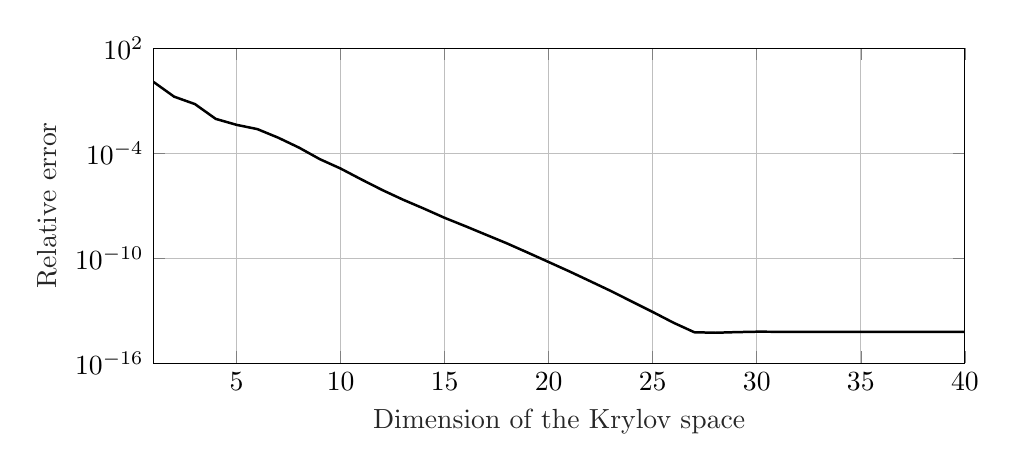
\begin{tikzpicture}

\begin{axis}[%
width=.85\linewidth,
height=4cm,
at={(0in,0in)},
scale only axis,
xmin=1,
xmax=40,
xlabel style={font=\color{white!15!black}},
xlabel={Dimension of the Krylov space},
ymode=log,
ymin=1e-16,
ymax=100,
yminorticks=true,
ylabel style={font=\color{white!15!black}},
ylabel={Relative error},
axis background/.style={fill=white},
xmajorgrids,
ymajorgrids,
yminorgrids,
legend style={legend cell align=left, align=left, draw=white!15!black}
]
\addplot [color=black, line width=0.9pt]
  table[row sep=crcr]{%
1	1.1970666841712\\
2	0.169080928746973\\
3	0.0636940730507964\\
4	0.00908042059055621\\
5	0.00414871323651826\\
6	0.00236609497417638\\
7	0.000766896348482475\\
8	0.000207499206291239\\
9	4.5468096002382e-05\\
10	1.3189262330513e-05\\
11	3.14525985651137e-06\\
12	7.83654425173314e-07\\
13	2.19404091753492e-07\\
14	6.80556241974471e-08\\
15	2.00761703179977e-08\\
16	6.68924820811396e-09\\
17	2.14505152308309e-09\\
18	6.93255504657795e-10\\
19	2.05483068858047e-10\\
20	5.98199450964638e-11\\
21	1.73494311883148e-11\\
22	4.77956305951699e-12\\
23	1.30520399685991e-12\\
24	3.28540461009388e-13\\
25	8.38065195569727e-14\\
26	2.03158589692223e-14\\
27	5.81332239277395e-15\\
28	5.44489077592386e-15\\
29	5.8980465774604e-15\\
30	6.23518964189752e-15\\
31	6.19390114291783e-15\\
32	6.11805363564131e-15\\
33	6.09205637160788e-15\\
34	6.14371904504169e-15\\
35	6.17541894368464e-15\\
36	6.12644428023124e-15\\
37	6.09499001710448e-15\\
38	6.1465375480684e-15\\
39	6.11087985201717e-15\\
40	6.12885950388518e-15\\
};
%\addlegendentry{data1}

\end{axis}
\end{tikzpicture}%
        \caption{}
        \label{fig:ode_conv}
    \end{subfigure}\hspace{.05\linewidth}
    \begin{subfigure}[b]{.45\linewidth}
        % This file was created by matlab2tikz.
%
%The latest updates can be retrieved from
%  http://www.mathworks.com/matlabcentral/fileexchange/22022-matlab2tikz-matlab2tikz
%where you can also make suggestions and rate matlab2tikz.
%
\begin{tikzpicture}

\begin{axis}[%
width=.85\linewidth,
height=4cm,
at={(0in,0in)},
scale only axis,
xmin=0,
xmax=2501,
xlabel style={font=\color{white!15!black}},
xlabel={nz = 12300},
y dir=reverse,
ymin=0,
ymax=2501,
axis background/.style={fill=white},
legend style={legend cell align=left, align=left, draw=white!15!black}
]
\addplot [color=black, draw=none, mark size=0.7pt, mark=*, mark options={solid, black}, forget plot]
  table[row sep=crcr]{%
1	1\\
1	2\\
1	51\\
2	1\\
2	2\\
2	3\\
2	52\\
3	2\\
3	3\\
3	4\\
3	53\\
4	3\\
4	4\\
4	5\\
4	54\\
5	4\\
5	5\\
5	6\\
5	55\\
6	5\\
6	6\\
6	7\\
6	56\\
7	6\\
7	7\\
7	8\\
7	57\\
8	7\\
8	8\\
8	9\\
8	58\\
9	8\\
9	9\\
9	10\\
9	59\\
10	9\\
10	10\\
10	11\\
10	60\\
11	10\\
11	11\\
11	12\\
11	61\\
12	11\\
12	12\\
12	13\\
12	62\\
13	12\\
13	13\\
13	14\\
13	63\\
14	13\\
14	14\\
14	15\\
14	64\\
15	14\\
15	15\\
15	16\\
15	65\\
16	15\\
16	16\\
16	17\\
16	66\\
17	16\\
17	17\\
17	18\\
17	67\\
18	17\\
18	18\\
18	19\\
18	68\\
19	18\\
19	19\\
19	20\\
19	69\\
20	19\\
20	20\\
20	21\\
20	70\\
21	20\\
21	21\\
21	22\\
21	71\\
22	21\\
22	22\\
22	23\\
22	72\\
23	22\\
23	23\\
23	24\\
23	73\\
24	23\\
24	24\\
24	25\\
24	74\\
25	24\\
25	25\\
25	26\\
25	75\\
26	25\\
26	26\\
26	27\\
26	76\\
27	26\\
27	27\\
27	28\\
27	77\\
28	27\\
28	28\\
28	29\\
28	78\\
29	28\\
29	29\\
29	30\\
29	79\\
30	29\\
30	30\\
30	31\\
30	80\\
31	30\\
31	31\\
31	32\\
31	81\\
32	31\\
32	32\\
32	33\\
32	82\\
33	32\\
33	33\\
33	34\\
33	83\\
34	33\\
34	34\\
34	35\\
34	84\\
35	34\\
35	35\\
35	36\\
35	85\\
36	35\\
36	36\\
36	37\\
36	86\\
37	36\\
37	37\\
37	38\\
37	87\\
38	37\\
38	38\\
38	39\\
38	88\\
39	38\\
39	39\\
39	40\\
39	89\\
40	39\\
40	40\\
40	41\\
40	90\\
41	40\\
41	41\\
41	42\\
41	91\\
42	41\\
42	42\\
42	43\\
42	92\\
43	42\\
43	43\\
43	44\\
43	93\\
44	43\\
44	44\\
44	45\\
44	94\\
45	44\\
45	45\\
45	46\\
45	95\\
46	45\\
46	46\\
46	47\\
46	96\\
47	46\\
47	47\\
47	48\\
47	97\\
48	47\\
48	48\\
48	49\\
48	98\\
49	48\\
49	49\\
49	50\\
49	99\\
50	49\\
50	50\\
50	100\\
51	1\\
51	51\\
51	52\\
51	101\\
52	2\\
52	51\\
52	52\\
52	53\\
52	102\\
53	3\\
53	52\\
53	53\\
53	54\\
53	103\\
54	4\\
54	53\\
54	54\\
54	55\\
54	104\\
55	5\\
55	54\\
55	55\\
55	56\\
55	105\\
56	6\\
56	55\\
56	56\\
56	57\\
56	106\\
57	7\\
57	56\\
57	57\\
57	58\\
57	107\\
58	8\\
58	57\\
58	58\\
58	59\\
58	108\\
59	9\\
59	58\\
59	59\\
59	60\\
59	109\\
60	10\\
60	59\\
60	60\\
60	61\\
60	110\\
61	11\\
61	60\\
61	61\\
61	62\\
61	111\\
62	12\\
62	61\\
62	62\\
62	63\\
62	112\\
63	13\\
63	62\\
63	63\\
63	64\\
63	113\\
64	14\\
64	63\\
64	64\\
64	65\\
64	114\\
65	15\\
65	64\\
65	65\\
65	66\\
65	115\\
66	16\\
66	65\\
66	66\\
66	67\\
66	116\\
67	17\\
67	66\\
67	67\\
67	68\\
67	117\\
68	18\\
68	67\\
68	68\\
68	69\\
68	118\\
69	19\\
69	68\\
69	69\\
69	70\\
69	119\\
70	20\\
70	69\\
70	70\\
70	71\\
70	120\\
71	21\\
71	70\\
71	71\\
71	72\\
71	121\\
72	22\\
72	71\\
72	72\\
72	73\\
72	122\\
73	23\\
73	72\\
73	73\\
73	74\\
73	123\\
74	24\\
74	73\\
74	74\\
74	75\\
74	124\\
75	25\\
75	74\\
75	75\\
75	76\\
75	125\\
76	26\\
76	75\\
76	76\\
76	77\\
76	126\\
77	27\\
77	76\\
77	77\\
77	78\\
77	127\\
78	28\\
78	77\\
78	78\\
78	79\\
78	128\\
79	29\\
79	78\\
79	79\\
79	80\\
79	129\\
80	30\\
80	79\\
80	80\\
80	81\\
80	130\\
81	31\\
81	80\\
81	81\\
81	82\\
81	131\\
82	32\\
82	81\\
82	82\\
82	83\\
82	132\\
83	33\\
83	82\\
83	83\\
83	84\\
83	133\\
84	34\\
84	83\\
84	84\\
84	85\\
84	134\\
85	35\\
85	84\\
85	85\\
85	86\\
85	135\\
86	36\\
86	85\\
86	86\\
86	87\\
86	136\\
87	37\\
87	86\\
87	87\\
87	88\\
87	137\\
88	38\\
88	87\\
88	88\\
88	89\\
88	138\\
89	39\\
89	88\\
89	89\\
89	90\\
89	139\\
90	40\\
90	89\\
90	90\\
90	91\\
90	140\\
91	41\\
91	90\\
91	91\\
91	92\\
91	141\\
92	42\\
92	91\\
92	92\\
92	93\\
92	142\\
93	43\\
93	92\\
93	93\\
93	94\\
93	143\\
94	44\\
94	93\\
94	94\\
94	95\\
94	144\\
95	45\\
95	94\\
95	95\\
95	96\\
95	145\\
96	46\\
96	95\\
96	96\\
96	97\\
96	146\\
97	47\\
97	96\\
97	97\\
97	98\\
97	147\\
98	48\\
98	97\\
98	98\\
98	99\\
98	148\\
99	49\\
99	98\\
99	99\\
99	100\\
99	149\\
100	50\\
100	99\\
100	100\\
100	150\\
101	51\\
101	101\\
101	102\\
101	151\\
102	52\\
102	101\\
102	102\\
102	103\\
102	152\\
103	53\\
103	102\\
103	103\\
103	104\\
103	153\\
104	54\\
104	103\\
104	104\\
104	105\\
104	154\\
105	55\\
105	104\\
105	105\\
105	106\\
105	155\\
106	56\\
106	105\\
106	106\\
106	107\\
106	156\\
107	57\\
107	106\\
107	107\\
107	108\\
107	157\\
108	58\\
108	107\\
108	108\\
108	109\\
108	158\\
109	59\\
109	108\\
109	109\\
109	110\\
109	159\\
110	60\\
110	109\\
110	110\\
110	111\\
110	160\\
111	61\\
111	110\\
111	111\\
111	112\\
111	161\\
112	62\\
112	111\\
112	112\\
112	113\\
112	162\\
113	63\\
113	112\\
113	113\\
113	114\\
113	163\\
114	64\\
114	113\\
114	114\\
114	115\\
114	164\\
115	65\\
115	114\\
115	115\\
115	116\\
115	165\\
116	66\\
116	115\\
116	116\\
116	117\\
116	166\\
117	67\\
117	116\\
117	117\\
117	118\\
117	167\\
118	68\\
118	117\\
118	118\\
118	119\\
118	168\\
119	69\\
119	118\\
119	119\\
119	120\\
119	169\\
120	70\\
120	119\\
120	120\\
120	121\\
120	170\\
121	71\\
121	120\\
121	121\\
121	122\\
121	171\\
122	72\\
122	121\\
122	122\\
122	123\\
122	172\\
123	73\\
123	122\\
123	123\\
123	124\\
123	173\\
124	74\\
124	123\\
124	124\\
124	125\\
124	174\\
125	75\\
125	124\\
125	125\\
125	126\\
125	175\\
126	76\\
126	125\\
126	126\\
126	127\\
126	176\\
127	77\\
127	126\\
127	127\\
127	128\\
127	177\\
128	78\\
128	127\\
128	128\\
128	129\\
128	178\\
129	79\\
129	128\\
129	129\\
129	130\\
129	179\\
130	80\\
130	129\\
130	130\\
130	131\\
130	180\\
131	81\\
131	130\\
131	131\\
131	132\\
131	181\\
132	82\\
132	131\\
132	132\\
132	133\\
132	182\\
133	83\\
133	132\\
133	133\\
133	134\\
133	183\\
134	84\\
134	133\\
134	134\\
134	135\\
134	184\\
135	85\\
135	134\\
135	135\\
135	136\\
135	185\\
136	86\\
136	135\\
136	136\\
136	137\\
136	186\\
137	87\\
137	136\\
137	137\\
137	138\\
137	187\\
138	88\\
138	137\\
138	138\\
138	139\\
138	188\\
139	89\\
139	138\\
139	139\\
139	140\\
139	189\\
140	90\\
140	139\\
140	140\\
140	141\\
140	190\\
141	91\\
141	140\\
141	141\\
141	142\\
141	191\\
142	92\\
142	141\\
142	142\\
142	143\\
142	192\\
143	93\\
143	142\\
143	143\\
143	144\\
143	193\\
144	94\\
144	143\\
144	144\\
144	145\\
144	194\\
145	95\\
145	144\\
145	145\\
145	146\\
145	195\\
146	96\\
146	145\\
146	146\\
146	147\\
146	196\\
147	97\\
147	146\\
147	147\\
147	148\\
147	197\\
148	98\\
148	147\\
148	148\\
148	149\\
148	198\\
149	99\\
149	148\\
149	149\\
149	150\\
149	199\\
150	100\\
150	149\\
150	150\\
150	200\\
151	101\\
151	151\\
151	152\\
151	201\\
152	102\\
152	151\\
152	152\\
152	153\\
152	202\\
153	103\\
153	152\\
153	153\\
153	154\\
153	203\\
154	104\\
154	153\\
154	154\\
154	155\\
154	204\\
155	105\\
155	154\\
155	155\\
155	156\\
155	205\\
156	106\\
156	155\\
156	156\\
156	157\\
156	206\\
157	107\\
157	156\\
157	157\\
157	158\\
157	207\\
158	108\\
158	157\\
158	158\\
158	159\\
158	208\\
159	109\\
159	158\\
159	159\\
159	160\\
159	209\\
160	110\\
160	159\\
160	160\\
160	161\\
160	210\\
161	111\\
161	160\\
161	161\\
161	162\\
161	211\\
162	112\\
162	161\\
162	162\\
162	163\\
162	212\\
163	113\\
163	162\\
163	163\\
163	164\\
163	213\\
164	114\\
164	163\\
164	164\\
164	165\\
164	214\\
165	115\\
165	164\\
165	165\\
165	166\\
165	215\\
166	116\\
166	165\\
166	166\\
166	167\\
166	216\\
167	117\\
167	166\\
167	167\\
167	168\\
167	217\\
168	118\\
168	167\\
168	168\\
168	169\\
168	218\\
169	119\\
169	168\\
169	169\\
169	170\\
169	219\\
170	120\\
170	169\\
170	170\\
170	171\\
170	220\\
171	121\\
171	170\\
171	171\\
171	172\\
171	221\\
172	122\\
172	171\\
172	172\\
172	173\\
172	222\\
173	123\\
173	172\\
173	173\\
173	174\\
173	223\\
174	124\\
174	173\\
174	174\\
174	175\\
174	224\\
175	125\\
175	174\\
175	175\\
175	176\\
175	225\\
176	126\\
176	175\\
176	176\\
176	177\\
176	226\\
177	127\\
177	176\\
177	177\\
177	178\\
177	227\\
178	128\\
178	177\\
178	178\\
178	179\\
178	228\\
179	129\\
179	178\\
179	179\\
179	180\\
179	229\\
180	130\\
180	179\\
180	180\\
180	181\\
180	230\\
181	131\\
181	180\\
181	181\\
181	182\\
181	231\\
182	132\\
182	181\\
182	182\\
182	183\\
182	232\\
183	133\\
183	182\\
183	183\\
183	184\\
183	233\\
184	134\\
184	183\\
184	184\\
184	185\\
184	234\\
185	135\\
185	184\\
185	185\\
185	186\\
185	235\\
186	136\\
186	185\\
186	186\\
186	187\\
186	236\\
187	137\\
187	186\\
187	187\\
187	188\\
187	237\\
188	138\\
188	187\\
188	188\\
188	189\\
188	238\\
189	139\\
189	188\\
189	189\\
189	190\\
189	239\\
190	140\\
190	189\\
190	190\\
190	191\\
190	240\\
191	141\\
191	190\\
191	191\\
191	192\\
191	241\\
192	142\\
192	191\\
192	192\\
192	193\\
192	242\\
193	143\\
193	192\\
193	193\\
193	194\\
193	243\\
194	144\\
194	193\\
194	194\\
194	195\\
194	244\\
195	145\\
195	194\\
195	195\\
195	196\\
195	245\\
196	146\\
196	195\\
196	196\\
196	197\\
196	246\\
197	147\\
197	196\\
197	197\\
197	198\\
197	247\\
198	148\\
198	197\\
198	198\\
198	199\\
198	248\\
199	149\\
199	198\\
199	199\\
199	200\\
199	249\\
200	150\\
200	199\\
200	200\\
200	250\\
201	151\\
201	201\\
201	202\\
201	251\\
202	152\\
202	201\\
202	202\\
202	203\\
202	252\\
203	153\\
203	202\\
203	203\\
203	204\\
203	253\\
204	154\\
204	203\\
204	204\\
204	205\\
204	254\\
205	155\\
205	204\\
205	205\\
205	206\\
205	255\\
206	156\\
206	205\\
206	206\\
206	207\\
206	256\\
207	157\\
207	206\\
207	207\\
207	208\\
207	257\\
208	158\\
208	207\\
208	208\\
208	209\\
208	258\\
209	159\\
209	208\\
209	209\\
209	210\\
209	259\\
210	160\\
210	209\\
210	210\\
210	211\\
210	260\\
211	161\\
211	210\\
211	211\\
211	212\\
211	261\\
212	162\\
212	211\\
212	212\\
212	213\\
212	262\\
213	163\\
213	212\\
213	213\\
213	214\\
213	263\\
214	164\\
214	213\\
214	214\\
214	215\\
214	264\\
215	165\\
215	214\\
215	215\\
215	216\\
215	265\\
216	166\\
216	215\\
216	216\\
216	217\\
216	266\\
217	167\\
217	216\\
217	217\\
217	218\\
217	267\\
218	168\\
218	217\\
218	218\\
218	219\\
218	268\\
219	169\\
219	218\\
219	219\\
219	220\\
219	269\\
220	170\\
220	219\\
220	220\\
220	221\\
220	270\\
221	171\\
221	220\\
221	221\\
221	222\\
221	271\\
222	172\\
222	221\\
222	222\\
222	223\\
222	272\\
223	173\\
223	222\\
223	223\\
223	224\\
223	273\\
224	174\\
224	223\\
224	224\\
224	225\\
224	274\\
225	175\\
225	224\\
225	225\\
225	226\\
225	275\\
226	176\\
226	225\\
226	226\\
226	227\\
226	276\\
227	177\\
227	226\\
227	227\\
227	228\\
227	277\\
228	178\\
228	227\\
228	228\\
228	229\\
228	278\\
229	179\\
229	228\\
229	229\\
229	230\\
229	279\\
230	180\\
230	229\\
230	230\\
230	231\\
230	280\\
231	181\\
231	230\\
231	231\\
231	232\\
231	281\\
232	182\\
232	231\\
232	232\\
232	233\\
232	282\\
233	183\\
233	232\\
233	233\\
233	234\\
233	283\\
234	184\\
234	233\\
234	234\\
234	235\\
234	284\\
235	185\\
235	234\\
235	235\\
235	236\\
235	285\\
236	186\\
236	235\\
236	236\\
236	237\\
236	286\\
237	187\\
237	236\\
237	237\\
237	238\\
237	287\\
238	188\\
238	237\\
238	238\\
238	239\\
238	288\\
239	189\\
239	238\\
239	239\\
239	240\\
239	289\\
240	190\\
240	239\\
240	240\\
240	241\\
240	290\\
241	191\\
241	240\\
241	241\\
241	242\\
241	291\\
242	192\\
242	241\\
242	242\\
242	243\\
242	292\\
243	193\\
243	242\\
243	243\\
243	244\\
243	293\\
244	194\\
244	243\\
244	244\\
244	245\\
244	294\\
245	195\\
245	244\\
245	245\\
245	246\\
245	295\\
246	196\\
246	245\\
246	246\\
246	247\\
246	296\\
247	197\\
247	246\\
247	247\\
247	248\\
247	297\\
248	198\\
248	247\\
248	248\\
248	249\\
248	298\\
249	199\\
249	248\\
249	249\\
249	250\\
249	299\\
250	200\\
250	249\\
250	250\\
250	300\\
251	201\\
251	251\\
251	252\\
251	301\\
252	202\\
252	251\\
252	252\\
252	253\\
252	302\\
253	203\\
253	252\\
253	253\\
253	254\\
253	303\\
254	204\\
254	253\\
254	254\\
254	255\\
254	304\\
255	205\\
255	254\\
255	255\\
255	256\\
255	305\\
256	206\\
256	255\\
256	256\\
256	257\\
256	306\\
257	207\\
257	256\\
257	257\\
257	258\\
257	307\\
258	208\\
258	257\\
258	258\\
258	259\\
258	308\\
259	209\\
259	258\\
259	259\\
259	260\\
259	309\\
260	210\\
260	259\\
260	260\\
260	261\\
260	310\\
261	211\\
261	260\\
261	261\\
261	262\\
261	311\\
262	212\\
262	261\\
262	262\\
262	263\\
262	312\\
263	213\\
263	262\\
263	263\\
263	264\\
263	313\\
264	214\\
264	263\\
264	264\\
264	265\\
264	314\\
265	215\\
265	264\\
265	265\\
265	266\\
265	315\\
266	216\\
266	265\\
266	266\\
266	267\\
266	316\\
267	217\\
267	266\\
267	267\\
267	268\\
267	317\\
268	218\\
268	267\\
268	268\\
268	269\\
268	318\\
269	219\\
269	268\\
269	269\\
269	270\\
269	319\\
270	220\\
270	269\\
270	270\\
270	271\\
270	320\\
271	221\\
271	270\\
271	271\\
271	272\\
271	321\\
272	222\\
272	271\\
272	272\\
272	273\\
272	322\\
273	223\\
273	272\\
273	273\\
273	274\\
273	323\\
274	224\\
274	273\\
274	274\\
274	275\\
274	324\\
275	225\\
275	274\\
275	275\\
275	276\\
275	325\\
276	226\\
276	275\\
276	276\\
276	277\\
276	326\\
277	227\\
277	276\\
277	277\\
277	278\\
277	327\\
278	228\\
278	277\\
278	278\\
278	279\\
278	328\\
279	229\\
279	278\\
279	279\\
279	280\\
279	329\\
280	230\\
280	279\\
280	280\\
280	281\\
280	330\\
281	231\\
281	280\\
281	281\\
281	282\\
281	331\\
282	232\\
282	281\\
282	282\\
282	283\\
282	332\\
283	233\\
283	282\\
283	283\\
283	284\\
283	333\\
284	234\\
284	283\\
284	284\\
284	285\\
284	334\\
285	235\\
285	284\\
285	285\\
285	286\\
285	335\\
286	236\\
286	285\\
286	286\\
286	287\\
286	336\\
287	237\\
287	286\\
287	287\\
287	288\\
287	337\\
288	238\\
288	287\\
288	288\\
288	289\\
288	338\\
289	239\\
289	288\\
289	289\\
289	290\\
289	339\\
290	240\\
290	289\\
290	290\\
290	291\\
290	340\\
291	241\\
291	290\\
291	291\\
291	292\\
291	341\\
292	242\\
292	291\\
292	292\\
292	293\\
292	342\\
293	243\\
293	292\\
293	293\\
293	294\\
293	343\\
294	244\\
294	293\\
294	294\\
294	295\\
294	344\\
295	245\\
295	294\\
295	295\\
295	296\\
295	345\\
296	246\\
296	295\\
296	296\\
296	297\\
296	346\\
297	247\\
297	296\\
297	297\\
297	298\\
297	347\\
298	248\\
298	297\\
298	298\\
298	299\\
298	348\\
299	249\\
299	298\\
299	299\\
299	300\\
299	349\\
300	250\\
300	299\\
300	300\\
300	350\\
301	251\\
301	301\\
301	302\\
301	351\\
302	252\\
302	301\\
302	302\\
302	303\\
302	352\\
303	253\\
303	302\\
303	303\\
303	304\\
303	353\\
304	254\\
304	303\\
304	304\\
304	305\\
304	354\\
305	255\\
305	304\\
305	305\\
305	306\\
305	355\\
306	256\\
306	305\\
306	306\\
306	307\\
306	356\\
307	257\\
307	306\\
307	307\\
307	308\\
307	357\\
308	258\\
308	307\\
308	308\\
308	309\\
308	358\\
309	259\\
309	308\\
309	309\\
309	310\\
309	359\\
310	260\\
310	309\\
310	310\\
310	311\\
310	360\\
311	261\\
311	310\\
311	311\\
311	312\\
311	361\\
312	262\\
312	311\\
312	312\\
312	313\\
312	362\\
313	263\\
313	312\\
313	313\\
313	314\\
313	363\\
314	264\\
314	313\\
314	314\\
314	315\\
314	364\\
315	265\\
315	314\\
315	315\\
315	316\\
315	365\\
316	266\\
316	315\\
316	316\\
316	317\\
316	366\\
317	267\\
317	316\\
317	317\\
317	318\\
317	367\\
318	268\\
318	317\\
318	318\\
318	319\\
318	368\\
319	269\\
319	318\\
319	319\\
319	320\\
319	369\\
320	270\\
320	319\\
320	320\\
320	321\\
320	370\\
321	271\\
321	320\\
321	321\\
321	322\\
321	371\\
322	272\\
322	321\\
322	322\\
322	323\\
322	372\\
323	273\\
323	322\\
323	323\\
323	324\\
323	373\\
324	274\\
324	323\\
324	324\\
324	325\\
324	374\\
325	275\\
325	324\\
325	325\\
325	326\\
325	375\\
326	276\\
326	325\\
326	326\\
326	327\\
326	376\\
327	277\\
327	326\\
327	327\\
327	328\\
327	377\\
328	278\\
328	327\\
328	328\\
328	329\\
328	378\\
329	279\\
329	328\\
329	329\\
329	330\\
329	379\\
330	280\\
330	329\\
330	330\\
330	331\\
330	380\\
331	281\\
331	330\\
331	331\\
331	332\\
331	381\\
332	282\\
332	331\\
332	332\\
332	333\\
332	382\\
333	283\\
333	332\\
333	333\\
333	334\\
333	383\\
334	284\\
334	333\\
334	334\\
334	335\\
334	384\\
335	285\\
335	334\\
335	335\\
335	336\\
335	385\\
336	286\\
336	335\\
336	336\\
336	337\\
336	386\\
337	287\\
337	336\\
337	337\\
337	338\\
337	387\\
338	288\\
338	337\\
338	338\\
338	339\\
338	388\\
339	289\\
339	338\\
339	339\\
339	340\\
339	389\\
340	290\\
340	339\\
340	340\\
340	341\\
340	390\\
341	291\\
341	340\\
341	341\\
341	342\\
341	391\\
342	292\\
342	341\\
342	342\\
342	343\\
342	392\\
343	293\\
343	342\\
343	343\\
343	344\\
343	393\\
344	294\\
344	343\\
344	344\\
344	345\\
344	394\\
345	295\\
345	344\\
345	345\\
345	346\\
345	395\\
346	296\\
346	345\\
346	346\\
346	347\\
346	396\\
347	297\\
347	346\\
347	347\\
347	348\\
347	397\\
348	298\\
348	347\\
348	348\\
348	349\\
348	398\\
349	299\\
349	348\\
349	349\\
349	350\\
349	399\\
350	300\\
350	349\\
350	350\\
350	400\\
351	301\\
351	351\\
351	352\\
351	401\\
352	302\\
352	351\\
352	352\\
352	353\\
352	402\\
353	303\\
353	352\\
353	353\\
353	354\\
353	403\\
354	304\\
354	353\\
354	354\\
354	355\\
354	404\\
355	305\\
355	354\\
355	355\\
355	356\\
355	405\\
356	306\\
356	355\\
356	356\\
356	357\\
356	406\\
357	307\\
357	356\\
357	357\\
357	358\\
357	407\\
358	308\\
358	357\\
358	358\\
358	359\\
358	408\\
359	309\\
359	358\\
359	359\\
359	360\\
359	409\\
360	310\\
360	359\\
360	360\\
360	361\\
360	410\\
361	311\\
361	360\\
361	361\\
361	362\\
361	411\\
362	312\\
362	361\\
362	362\\
362	363\\
362	412\\
363	313\\
363	362\\
363	363\\
363	364\\
363	413\\
364	314\\
364	363\\
364	364\\
364	365\\
364	414\\
365	315\\
365	364\\
365	365\\
365	366\\
365	415\\
366	316\\
366	365\\
366	366\\
366	367\\
366	416\\
367	317\\
367	366\\
367	367\\
367	368\\
367	417\\
368	318\\
368	367\\
368	368\\
368	369\\
368	418\\
369	319\\
369	368\\
369	369\\
369	370\\
369	419\\
370	320\\
370	369\\
370	370\\
370	371\\
370	420\\
371	321\\
371	370\\
371	371\\
371	372\\
371	421\\
372	322\\
372	371\\
372	372\\
372	373\\
372	422\\
373	323\\
373	372\\
373	373\\
373	374\\
373	423\\
374	324\\
374	373\\
374	374\\
374	375\\
374	424\\
375	325\\
375	374\\
375	375\\
375	376\\
375	425\\
376	326\\
376	375\\
376	376\\
376	377\\
376	426\\
377	327\\
377	376\\
377	377\\
377	378\\
377	427\\
378	328\\
378	377\\
378	378\\
378	379\\
378	428\\
379	329\\
379	378\\
379	379\\
379	380\\
379	429\\
380	330\\
380	379\\
380	380\\
380	381\\
380	430\\
381	331\\
381	380\\
381	381\\
381	382\\
381	431\\
382	332\\
382	381\\
382	382\\
382	383\\
382	432\\
383	333\\
383	382\\
383	383\\
383	384\\
383	433\\
384	334\\
384	383\\
384	384\\
384	385\\
384	434\\
385	335\\
385	384\\
385	385\\
385	386\\
385	435\\
386	336\\
386	385\\
386	386\\
386	387\\
386	436\\
387	337\\
387	386\\
387	387\\
387	388\\
387	437\\
388	338\\
388	387\\
388	388\\
388	389\\
388	438\\
389	339\\
389	388\\
389	389\\
389	390\\
389	439\\
390	340\\
390	389\\
390	390\\
390	391\\
390	440\\
391	341\\
391	390\\
391	391\\
391	392\\
391	441\\
392	342\\
392	391\\
392	392\\
392	393\\
392	442\\
393	343\\
393	392\\
393	393\\
393	394\\
393	443\\
394	344\\
394	393\\
394	394\\
394	395\\
394	444\\
395	345\\
395	394\\
395	395\\
395	396\\
395	445\\
396	346\\
396	395\\
396	396\\
396	397\\
396	446\\
397	347\\
397	396\\
397	397\\
397	398\\
397	447\\
398	348\\
398	397\\
398	398\\
398	399\\
398	448\\
399	349\\
399	398\\
399	399\\
399	400\\
399	449\\
400	350\\
400	399\\
400	400\\
400	450\\
401	351\\
401	401\\
401	402\\
401	451\\
402	352\\
402	401\\
402	402\\
402	403\\
402	452\\
403	353\\
403	402\\
403	403\\
403	404\\
403	453\\
404	354\\
404	403\\
404	404\\
404	405\\
404	454\\
405	355\\
405	404\\
405	405\\
405	406\\
405	455\\
406	356\\
406	405\\
406	406\\
406	407\\
406	456\\
407	357\\
407	406\\
407	407\\
407	408\\
407	457\\
408	358\\
408	407\\
408	408\\
408	409\\
408	458\\
409	359\\
409	408\\
409	409\\
409	410\\
409	459\\
410	360\\
410	409\\
410	410\\
410	411\\
410	460\\
411	361\\
411	410\\
411	411\\
411	412\\
411	461\\
412	362\\
412	411\\
412	412\\
412	413\\
412	462\\
413	363\\
413	412\\
413	413\\
413	414\\
413	463\\
414	364\\
414	413\\
414	414\\
414	415\\
414	464\\
415	365\\
415	414\\
415	415\\
415	416\\
415	465\\
416	366\\
416	415\\
416	416\\
416	417\\
416	466\\
417	367\\
417	416\\
417	417\\
417	418\\
417	467\\
418	368\\
418	417\\
418	418\\
418	419\\
418	468\\
419	369\\
419	418\\
419	419\\
419	420\\
419	469\\
420	370\\
420	419\\
420	420\\
420	421\\
420	470\\
421	371\\
421	420\\
421	421\\
421	422\\
421	471\\
422	372\\
422	421\\
422	422\\
422	423\\
422	472\\
423	373\\
423	422\\
423	423\\
423	424\\
423	473\\
424	374\\
424	423\\
424	424\\
424	425\\
424	474\\
425	375\\
425	424\\
425	425\\
425	426\\
425	475\\
426	376\\
426	425\\
426	426\\
426	427\\
426	476\\
427	377\\
427	426\\
427	427\\
427	428\\
427	477\\
428	378\\
428	427\\
428	428\\
428	429\\
428	478\\
429	379\\
429	428\\
429	429\\
429	430\\
429	479\\
430	380\\
430	429\\
430	430\\
430	431\\
430	480\\
431	381\\
431	430\\
431	431\\
431	432\\
431	481\\
432	382\\
432	431\\
432	432\\
432	433\\
432	482\\
433	383\\
433	432\\
433	433\\
433	434\\
433	483\\
434	384\\
434	433\\
434	434\\
434	435\\
434	484\\
435	385\\
435	434\\
435	435\\
435	436\\
435	485\\
436	386\\
436	435\\
436	436\\
436	437\\
436	486\\
437	387\\
437	436\\
437	437\\
437	438\\
437	487\\
438	388\\
438	437\\
438	438\\
438	439\\
438	488\\
439	389\\
439	438\\
439	439\\
439	440\\
439	489\\
440	390\\
440	439\\
440	440\\
440	441\\
440	490\\
441	391\\
441	440\\
441	441\\
441	442\\
441	491\\
442	392\\
442	441\\
442	442\\
442	443\\
442	492\\
443	393\\
443	442\\
443	443\\
443	444\\
443	493\\
444	394\\
444	443\\
444	444\\
444	445\\
444	494\\
445	395\\
445	444\\
445	445\\
445	446\\
445	495\\
446	396\\
446	445\\
446	446\\
446	447\\
446	496\\
447	397\\
447	446\\
447	447\\
447	448\\
447	497\\
448	398\\
448	447\\
448	448\\
448	449\\
448	498\\
449	399\\
449	448\\
449	449\\
449	450\\
449	499\\
450	400\\
450	449\\
450	450\\
450	500\\
451	401\\
451	451\\
451	452\\
451	501\\
452	402\\
452	451\\
452	452\\
452	453\\
452	502\\
453	403\\
453	452\\
453	453\\
453	454\\
453	503\\
454	404\\
454	453\\
454	454\\
454	455\\
454	504\\
455	405\\
455	454\\
455	455\\
455	456\\
455	505\\
456	406\\
456	455\\
456	456\\
456	457\\
456	506\\
457	407\\
457	456\\
457	457\\
457	458\\
457	507\\
458	408\\
458	457\\
458	458\\
458	459\\
458	508\\
459	409\\
459	458\\
459	459\\
459	460\\
459	509\\
460	410\\
460	459\\
460	460\\
460	461\\
460	510\\
461	411\\
461	460\\
461	461\\
461	462\\
461	511\\
462	412\\
462	461\\
462	462\\
462	463\\
462	512\\
463	413\\
463	462\\
463	463\\
463	464\\
463	513\\
464	414\\
464	463\\
464	464\\
464	465\\
464	514\\
465	415\\
465	464\\
465	465\\
465	466\\
465	515\\
466	416\\
466	465\\
466	466\\
466	467\\
466	516\\
467	417\\
467	466\\
467	467\\
467	468\\
467	517\\
468	418\\
468	467\\
468	468\\
468	469\\
468	518\\
469	419\\
469	468\\
469	469\\
469	470\\
469	519\\
470	420\\
470	469\\
470	470\\
470	471\\
470	520\\
471	421\\
471	470\\
471	471\\
471	472\\
471	521\\
472	422\\
472	471\\
472	472\\
472	473\\
472	522\\
473	423\\
473	472\\
473	473\\
473	474\\
473	523\\
474	424\\
474	473\\
474	474\\
474	475\\
474	524\\
475	425\\
475	474\\
475	475\\
475	476\\
475	525\\
476	426\\
476	475\\
476	476\\
476	477\\
476	526\\
477	427\\
477	476\\
477	477\\
477	478\\
477	527\\
478	428\\
478	477\\
478	478\\
478	479\\
478	528\\
479	429\\
479	478\\
479	479\\
479	480\\
479	529\\
480	430\\
480	479\\
480	480\\
480	481\\
480	530\\
481	431\\
481	480\\
481	481\\
481	482\\
481	531\\
482	432\\
482	481\\
482	482\\
482	483\\
482	532\\
483	433\\
483	482\\
483	483\\
483	484\\
483	533\\
484	434\\
484	483\\
484	484\\
484	485\\
484	534\\
485	435\\
485	484\\
485	485\\
485	486\\
485	535\\
486	436\\
486	485\\
486	486\\
486	487\\
486	536\\
487	437\\
487	486\\
487	487\\
487	488\\
487	537\\
488	438\\
488	487\\
488	488\\
488	489\\
488	538\\
489	439\\
489	488\\
489	489\\
489	490\\
489	539\\
490	440\\
490	489\\
490	490\\
490	491\\
490	540\\
491	441\\
491	490\\
491	491\\
491	492\\
491	541\\
492	442\\
492	491\\
492	492\\
492	493\\
492	542\\
493	443\\
493	492\\
493	493\\
493	494\\
493	543\\
494	444\\
494	493\\
494	494\\
494	495\\
494	544\\
495	445\\
495	494\\
495	495\\
495	496\\
495	545\\
496	446\\
496	495\\
496	496\\
496	497\\
496	546\\
497	447\\
497	496\\
497	497\\
497	498\\
497	547\\
498	448\\
498	497\\
498	498\\
498	499\\
498	548\\
499	449\\
499	498\\
499	499\\
499	500\\
499	549\\
500	450\\
500	499\\
500	500\\
500	550\\
501	451\\
501	501\\
501	502\\
501	551\\
502	452\\
502	501\\
502	502\\
502	503\\
502	552\\
503	453\\
503	502\\
503	503\\
503	504\\
503	553\\
504	454\\
504	503\\
504	504\\
504	505\\
504	554\\
505	455\\
505	504\\
505	505\\
505	506\\
505	555\\
506	456\\
506	505\\
506	506\\
506	507\\
506	556\\
507	457\\
507	506\\
507	507\\
507	508\\
507	557\\
508	458\\
508	507\\
508	508\\
508	509\\
508	558\\
509	459\\
509	508\\
509	509\\
509	510\\
509	559\\
510	460\\
510	509\\
510	510\\
510	511\\
510	560\\
511	461\\
511	510\\
511	511\\
511	512\\
511	561\\
512	462\\
512	511\\
512	512\\
512	513\\
512	562\\
513	463\\
513	512\\
513	513\\
513	514\\
513	563\\
514	464\\
514	513\\
514	514\\
514	515\\
514	564\\
515	465\\
515	514\\
515	515\\
515	516\\
515	565\\
516	466\\
516	515\\
516	516\\
516	517\\
516	566\\
517	467\\
517	516\\
517	517\\
517	518\\
517	567\\
518	468\\
518	517\\
518	518\\
518	519\\
518	568\\
519	469\\
519	518\\
519	519\\
519	520\\
519	569\\
520	470\\
520	519\\
520	520\\
520	521\\
520	570\\
521	471\\
521	520\\
521	521\\
521	522\\
521	571\\
522	472\\
522	521\\
522	522\\
522	523\\
522	572\\
523	473\\
523	522\\
523	523\\
523	524\\
523	573\\
524	474\\
524	523\\
524	524\\
524	525\\
524	574\\
525	475\\
525	524\\
525	525\\
525	526\\
525	575\\
526	476\\
526	525\\
526	526\\
526	527\\
526	576\\
527	477\\
527	526\\
527	527\\
527	528\\
527	577\\
528	478\\
528	527\\
528	528\\
528	529\\
528	578\\
529	479\\
529	528\\
529	529\\
529	530\\
529	579\\
530	480\\
530	529\\
530	530\\
530	531\\
530	580\\
531	481\\
531	530\\
531	531\\
531	532\\
531	581\\
532	482\\
532	531\\
532	532\\
532	533\\
532	582\\
533	483\\
533	532\\
533	533\\
533	534\\
533	583\\
534	484\\
534	533\\
534	534\\
534	535\\
534	584\\
535	485\\
535	534\\
535	535\\
535	536\\
535	585\\
536	486\\
536	535\\
536	536\\
536	537\\
536	586\\
537	487\\
537	536\\
537	537\\
537	538\\
537	587\\
538	488\\
538	537\\
538	538\\
538	539\\
538	588\\
539	489\\
539	538\\
539	539\\
539	540\\
539	589\\
540	490\\
540	539\\
540	540\\
540	541\\
540	590\\
541	491\\
541	540\\
541	541\\
541	542\\
541	591\\
542	492\\
542	541\\
542	542\\
542	543\\
542	592\\
543	493\\
543	542\\
543	543\\
543	544\\
543	593\\
544	494\\
544	543\\
544	544\\
544	545\\
544	594\\
545	495\\
545	544\\
545	545\\
545	546\\
545	595\\
546	496\\
546	545\\
546	546\\
546	547\\
546	596\\
547	497\\
547	546\\
547	547\\
547	548\\
547	597\\
548	498\\
548	547\\
548	548\\
548	549\\
548	598\\
549	499\\
549	548\\
549	549\\
549	550\\
549	599\\
550	500\\
550	549\\
550	550\\
550	600\\
551	501\\
551	551\\
551	552\\
551	601\\
552	502\\
552	551\\
552	552\\
552	553\\
552	602\\
553	503\\
553	552\\
553	553\\
553	554\\
553	603\\
554	504\\
554	553\\
554	554\\
554	555\\
554	604\\
555	505\\
555	554\\
555	555\\
555	556\\
555	605\\
556	506\\
556	555\\
556	556\\
556	557\\
556	606\\
557	507\\
557	556\\
557	557\\
557	558\\
557	607\\
558	508\\
558	557\\
558	558\\
558	559\\
558	608\\
559	509\\
559	558\\
559	559\\
559	560\\
559	609\\
560	510\\
560	559\\
560	560\\
560	561\\
560	610\\
561	511\\
561	560\\
561	561\\
561	562\\
561	611\\
562	512\\
562	561\\
562	562\\
562	563\\
562	612\\
563	513\\
563	562\\
563	563\\
563	564\\
563	613\\
564	514\\
564	563\\
564	564\\
564	565\\
564	614\\
565	515\\
565	564\\
565	565\\
565	566\\
565	615\\
566	516\\
566	565\\
566	566\\
566	567\\
566	616\\
567	517\\
567	566\\
567	567\\
567	568\\
567	617\\
568	518\\
568	567\\
568	568\\
568	569\\
568	618\\
569	519\\
569	568\\
569	569\\
569	570\\
569	619\\
570	520\\
570	569\\
570	570\\
570	571\\
570	620\\
571	521\\
571	570\\
571	571\\
571	572\\
571	621\\
572	522\\
572	571\\
572	572\\
572	573\\
572	622\\
573	523\\
573	572\\
573	573\\
573	574\\
573	623\\
574	524\\
574	573\\
574	574\\
574	575\\
574	624\\
575	525\\
575	574\\
575	575\\
575	576\\
575	625\\
576	526\\
576	575\\
576	576\\
576	577\\
576	626\\
577	527\\
577	576\\
577	577\\
577	578\\
577	627\\
578	528\\
578	577\\
578	578\\
578	579\\
578	628\\
579	529\\
579	578\\
579	579\\
579	580\\
579	629\\
580	530\\
580	579\\
580	580\\
580	581\\
580	630\\
581	531\\
581	580\\
581	581\\
581	582\\
581	631\\
582	532\\
582	581\\
582	582\\
582	583\\
582	632\\
583	533\\
583	582\\
583	583\\
583	584\\
583	633\\
584	534\\
584	583\\
584	584\\
584	585\\
584	634\\
585	535\\
585	584\\
585	585\\
585	586\\
585	635\\
586	536\\
586	585\\
586	586\\
586	587\\
586	636\\
587	537\\
587	586\\
587	587\\
587	588\\
587	637\\
588	538\\
588	587\\
588	588\\
588	589\\
588	638\\
589	539\\
589	588\\
589	589\\
589	590\\
589	639\\
590	540\\
590	589\\
590	590\\
590	591\\
590	640\\
591	541\\
591	590\\
591	591\\
591	592\\
591	641\\
592	542\\
592	591\\
592	592\\
592	593\\
592	642\\
593	543\\
593	592\\
593	593\\
593	594\\
593	643\\
594	544\\
594	593\\
594	594\\
594	595\\
594	644\\
595	545\\
595	594\\
595	595\\
595	596\\
595	645\\
596	546\\
596	595\\
596	596\\
596	597\\
596	646\\
597	547\\
597	596\\
597	597\\
597	598\\
597	647\\
598	548\\
598	597\\
598	598\\
598	599\\
598	648\\
599	549\\
599	598\\
599	599\\
599	600\\
599	649\\
600	550\\
600	599\\
600	600\\
600	650\\
601	551\\
601	601\\
601	602\\
601	651\\
602	552\\
602	601\\
602	602\\
602	603\\
602	652\\
603	553\\
603	602\\
603	603\\
603	604\\
603	653\\
604	554\\
604	603\\
604	604\\
604	605\\
604	654\\
605	555\\
605	604\\
605	605\\
605	606\\
605	655\\
606	556\\
606	605\\
606	606\\
606	607\\
606	656\\
607	557\\
607	606\\
607	607\\
607	608\\
607	657\\
608	558\\
608	607\\
608	608\\
608	609\\
608	658\\
609	559\\
609	608\\
609	609\\
609	610\\
609	659\\
610	560\\
610	609\\
610	610\\
610	611\\
610	660\\
611	561\\
611	610\\
611	611\\
611	612\\
611	661\\
612	562\\
612	611\\
612	612\\
612	613\\
612	662\\
613	563\\
613	612\\
613	613\\
613	614\\
613	663\\
614	564\\
614	613\\
614	614\\
614	615\\
614	664\\
615	565\\
615	614\\
615	615\\
615	616\\
615	665\\
616	566\\
616	615\\
616	616\\
616	617\\
616	666\\
617	567\\
617	616\\
617	617\\
617	618\\
617	667\\
618	568\\
618	617\\
618	618\\
618	619\\
618	668\\
619	569\\
619	618\\
619	619\\
619	620\\
619	669\\
620	570\\
620	619\\
620	620\\
620	621\\
620	670\\
621	571\\
621	620\\
621	621\\
621	622\\
621	671\\
622	572\\
622	621\\
622	622\\
622	623\\
622	672\\
623	573\\
623	622\\
623	623\\
623	624\\
623	673\\
624	574\\
624	623\\
624	624\\
624	625\\
624	674\\
625	575\\
625	624\\
625	625\\
625	626\\
625	675\\
626	576\\
626	625\\
626	626\\
626	627\\
626	676\\
627	577\\
627	626\\
627	627\\
627	628\\
627	677\\
628	578\\
628	627\\
628	628\\
628	629\\
628	678\\
629	579\\
629	628\\
629	629\\
629	630\\
629	679\\
630	580\\
630	629\\
630	630\\
630	631\\
630	680\\
631	581\\
631	630\\
631	631\\
631	632\\
631	681\\
632	582\\
632	631\\
632	632\\
632	633\\
632	682\\
633	583\\
633	632\\
633	633\\
633	634\\
633	683\\
634	584\\
634	633\\
634	634\\
634	635\\
634	684\\
635	585\\
635	634\\
635	635\\
635	636\\
635	685\\
636	586\\
636	635\\
636	636\\
636	637\\
636	686\\
637	587\\
637	636\\
637	637\\
637	638\\
637	687\\
638	588\\
638	637\\
638	638\\
638	639\\
638	688\\
639	589\\
639	638\\
639	639\\
639	640\\
639	689\\
640	590\\
640	639\\
640	640\\
640	641\\
640	690\\
641	591\\
641	640\\
641	641\\
641	642\\
641	691\\
642	592\\
642	641\\
642	642\\
642	643\\
642	692\\
643	593\\
643	642\\
643	643\\
643	644\\
643	693\\
644	594\\
644	643\\
644	644\\
644	645\\
644	694\\
645	595\\
645	644\\
645	645\\
645	646\\
645	695\\
646	596\\
646	645\\
646	646\\
646	647\\
646	696\\
647	597\\
647	646\\
647	647\\
647	648\\
647	697\\
648	598\\
648	647\\
648	648\\
648	649\\
648	698\\
649	599\\
649	648\\
649	649\\
649	650\\
649	699\\
650	600\\
650	649\\
650	650\\
650	700\\
651	601\\
651	651\\
651	652\\
651	701\\
652	602\\
652	651\\
652	652\\
652	653\\
652	702\\
653	603\\
653	652\\
653	653\\
653	654\\
653	703\\
654	604\\
654	653\\
654	654\\
654	655\\
654	704\\
655	605\\
655	654\\
655	655\\
655	656\\
655	705\\
656	606\\
656	655\\
656	656\\
656	657\\
656	706\\
657	607\\
657	656\\
657	657\\
657	658\\
657	707\\
658	608\\
658	657\\
658	658\\
658	659\\
658	708\\
659	609\\
659	658\\
659	659\\
659	660\\
659	709\\
660	610\\
660	659\\
660	660\\
660	661\\
660	710\\
661	611\\
661	660\\
661	661\\
661	662\\
661	711\\
662	612\\
662	661\\
662	662\\
662	663\\
662	712\\
663	613\\
663	662\\
663	663\\
663	664\\
663	713\\
664	614\\
664	663\\
664	664\\
664	665\\
664	714\\
665	615\\
665	664\\
665	665\\
665	666\\
665	715\\
666	616\\
666	665\\
666	666\\
666	667\\
666	716\\
667	617\\
667	666\\
667	667\\
667	668\\
667	717\\
668	618\\
668	667\\
668	668\\
668	669\\
668	718\\
669	619\\
669	668\\
669	669\\
669	670\\
669	719\\
670	620\\
670	669\\
670	670\\
670	671\\
670	720\\
671	621\\
671	670\\
671	671\\
671	672\\
671	721\\
672	622\\
672	671\\
672	672\\
672	673\\
672	722\\
673	623\\
673	672\\
673	673\\
673	674\\
673	723\\
674	624\\
674	673\\
674	674\\
674	675\\
674	724\\
675	625\\
675	674\\
675	675\\
675	676\\
675	725\\
676	626\\
676	675\\
676	676\\
676	677\\
676	726\\
677	627\\
677	676\\
677	677\\
677	678\\
677	727\\
678	628\\
678	677\\
678	678\\
678	679\\
678	728\\
679	629\\
679	678\\
679	679\\
679	680\\
679	729\\
680	630\\
680	679\\
680	680\\
680	681\\
680	730\\
681	631\\
681	680\\
681	681\\
681	682\\
681	731\\
682	632\\
682	681\\
682	682\\
682	683\\
682	732\\
683	633\\
683	682\\
683	683\\
683	684\\
683	733\\
684	634\\
684	683\\
684	684\\
684	685\\
684	734\\
685	635\\
685	684\\
685	685\\
685	686\\
685	735\\
686	636\\
686	685\\
686	686\\
686	687\\
686	736\\
687	637\\
687	686\\
687	687\\
687	688\\
687	737\\
688	638\\
688	687\\
688	688\\
688	689\\
688	738\\
689	639\\
689	688\\
689	689\\
689	690\\
689	739\\
690	640\\
690	689\\
690	690\\
690	691\\
690	740\\
691	641\\
691	690\\
691	691\\
691	692\\
691	741\\
692	642\\
692	691\\
692	692\\
692	693\\
692	742\\
693	643\\
693	692\\
693	693\\
693	694\\
693	743\\
694	644\\
694	693\\
694	694\\
694	695\\
694	744\\
695	645\\
695	694\\
695	695\\
695	696\\
695	745\\
696	646\\
696	695\\
696	696\\
696	697\\
696	746\\
697	647\\
697	696\\
697	697\\
697	698\\
697	747\\
698	648\\
698	697\\
698	698\\
698	699\\
698	748\\
699	649\\
699	698\\
699	699\\
699	700\\
699	749\\
700	650\\
700	699\\
700	700\\
700	750\\
701	651\\
701	701\\
701	702\\
701	751\\
702	652\\
702	701\\
702	702\\
702	703\\
702	752\\
703	653\\
703	702\\
703	703\\
703	704\\
703	753\\
704	654\\
704	703\\
704	704\\
704	705\\
704	754\\
705	655\\
705	704\\
705	705\\
705	706\\
705	755\\
706	656\\
706	705\\
706	706\\
706	707\\
706	756\\
707	657\\
707	706\\
707	707\\
707	708\\
707	757\\
708	658\\
708	707\\
708	708\\
708	709\\
708	758\\
709	659\\
709	708\\
709	709\\
709	710\\
709	759\\
710	660\\
710	709\\
710	710\\
710	711\\
710	760\\
711	661\\
711	710\\
711	711\\
711	712\\
711	761\\
712	662\\
712	711\\
712	712\\
712	713\\
712	762\\
713	663\\
713	712\\
713	713\\
713	714\\
713	763\\
714	664\\
714	713\\
714	714\\
714	715\\
714	764\\
715	665\\
715	714\\
715	715\\
715	716\\
715	765\\
716	666\\
716	715\\
716	716\\
716	717\\
716	766\\
717	667\\
717	716\\
717	717\\
717	718\\
717	767\\
718	668\\
718	717\\
718	718\\
718	719\\
718	768\\
719	669\\
719	718\\
719	719\\
719	720\\
719	769\\
720	670\\
720	719\\
720	720\\
720	721\\
720	770\\
721	671\\
721	720\\
721	721\\
721	722\\
721	771\\
722	672\\
722	721\\
722	722\\
722	723\\
722	772\\
723	673\\
723	722\\
723	723\\
723	724\\
723	773\\
724	674\\
724	723\\
724	724\\
724	725\\
724	774\\
725	675\\
725	724\\
725	725\\
725	726\\
725	775\\
726	676\\
726	725\\
726	726\\
726	727\\
726	776\\
727	677\\
727	726\\
727	727\\
727	728\\
727	777\\
728	678\\
728	727\\
728	728\\
728	729\\
728	778\\
729	679\\
729	728\\
729	729\\
729	730\\
729	779\\
730	680\\
730	729\\
730	730\\
730	731\\
730	780\\
731	681\\
731	730\\
731	731\\
731	732\\
731	781\\
732	682\\
732	731\\
732	732\\
732	733\\
732	782\\
733	683\\
733	732\\
733	733\\
733	734\\
733	783\\
734	684\\
734	733\\
734	734\\
734	735\\
734	784\\
735	685\\
735	734\\
735	735\\
735	736\\
735	785\\
736	686\\
736	735\\
736	736\\
736	737\\
736	786\\
737	687\\
737	736\\
737	737\\
737	738\\
737	787\\
738	688\\
738	737\\
738	738\\
738	739\\
738	788\\
739	689\\
739	738\\
739	739\\
739	740\\
739	789\\
740	690\\
740	739\\
740	740\\
740	741\\
740	790\\
741	691\\
741	740\\
741	741\\
741	742\\
741	791\\
742	692\\
742	741\\
742	742\\
742	743\\
742	792\\
743	693\\
743	742\\
743	743\\
743	744\\
743	793\\
744	694\\
744	743\\
744	744\\
744	745\\
744	794\\
745	695\\
745	744\\
745	745\\
745	746\\
745	795\\
746	696\\
746	745\\
746	746\\
746	747\\
746	796\\
747	697\\
747	746\\
747	747\\
747	748\\
747	797\\
748	698\\
748	747\\
748	748\\
748	749\\
748	798\\
749	699\\
749	748\\
749	749\\
749	750\\
749	799\\
750	700\\
750	749\\
750	750\\
750	800\\
751	701\\
751	751\\
751	752\\
751	801\\
752	702\\
752	751\\
752	752\\
752	753\\
752	802\\
753	703\\
753	752\\
753	753\\
753	754\\
753	803\\
754	704\\
754	753\\
754	754\\
754	755\\
754	804\\
755	705\\
755	754\\
755	755\\
755	756\\
755	805\\
756	706\\
756	755\\
756	756\\
756	757\\
756	806\\
757	707\\
757	756\\
757	757\\
757	758\\
757	807\\
758	708\\
758	757\\
758	758\\
758	759\\
758	808\\
759	709\\
759	758\\
759	759\\
759	760\\
759	809\\
760	710\\
760	759\\
760	760\\
760	761\\
760	810\\
761	711\\
761	760\\
761	761\\
761	762\\
761	811\\
762	712\\
762	761\\
762	762\\
762	763\\
762	812\\
763	713\\
763	762\\
763	763\\
763	764\\
763	813\\
764	714\\
764	763\\
764	764\\
764	765\\
764	814\\
765	715\\
765	764\\
765	765\\
765	766\\
765	815\\
766	716\\
766	765\\
766	766\\
766	767\\
766	816\\
767	717\\
767	766\\
767	767\\
767	768\\
767	817\\
768	718\\
768	767\\
768	768\\
768	769\\
768	818\\
769	719\\
769	768\\
769	769\\
769	770\\
769	819\\
770	720\\
770	769\\
770	770\\
770	771\\
770	820\\
771	721\\
771	770\\
771	771\\
771	772\\
771	821\\
772	722\\
772	771\\
772	772\\
772	773\\
772	822\\
773	723\\
773	772\\
773	773\\
773	774\\
773	823\\
774	724\\
774	773\\
774	774\\
774	775\\
774	824\\
775	725\\
775	774\\
775	775\\
775	776\\
775	825\\
776	726\\
776	775\\
776	776\\
776	777\\
776	826\\
777	727\\
777	776\\
777	777\\
777	778\\
777	827\\
778	728\\
778	777\\
778	778\\
778	779\\
778	828\\
779	729\\
779	778\\
779	779\\
779	780\\
779	829\\
780	730\\
780	779\\
780	780\\
780	781\\
780	830\\
781	731\\
781	780\\
781	781\\
781	782\\
781	831\\
782	732\\
782	781\\
782	782\\
782	783\\
782	832\\
783	733\\
783	782\\
783	783\\
783	784\\
783	833\\
784	734\\
784	783\\
784	784\\
784	785\\
784	834\\
785	735\\
785	784\\
785	785\\
785	786\\
785	835\\
786	736\\
786	785\\
786	786\\
786	787\\
786	836\\
787	737\\
787	786\\
787	787\\
787	788\\
787	837\\
788	738\\
788	787\\
788	788\\
788	789\\
788	838\\
789	739\\
789	788\\
789	789\\
789	790\\
789	839\\
790	740\\
790	789\\
790	790\\
790	791\\
790	840\\
791	741\\
791	790\\
791	791\\
791	792\\
791	841\\
792	742\\
792	791\\
792	792\\
792	793\\
792	842\\
793	743\\
793	792\\
793	793\\
793	794\\
793	843\\
794	744\\
794	793\\
794	794\\
794	795\\
794	844\\
795	745\\
795	794\\
795	795\\
795	796\\
795	845\\
796	746\\
796	795\\
796	796\\
796	797\\
796	846\\
797	747\\
797	796\\
797	797\\
797	798\\
797	847\\
798	748\\
798	797\\
798	798\\
798	799\\
798	848\\
799	749\\
799	798\\
799	799\\
799	800\\
799	849\\
800	750\\
800	799\\
800	800\\
800	850\\
801	751\\
801	801\\
801	802\\
801	851\\
802	752\\
802	801\\
802	802\\
802	803\\
802	852\\
803	753\\
803	802\\
803	803\\
803	804\\
803	853\\
804	754\\
804	803\\
804	804\\
804	805\\
804	854\\
805	755\\
805	804\\
805	805\\
805	806\\
805	855\\
806	756\\
806	805\\
806	806\\
806	807\\
806	856\\
807	757\\
807	806\\
807	807\\
807	808\\
807	857\\
808	758\\
808	807\\
808	808\\
808	809\\
808	858\\
809	759\\
809	808\\
809	809\\
809	810\\
809	859\\
810	760\\
810	809\\
810	810\\
810	811\\
810	860\\
811	761\\
811	810\\
811	811\\
811	812\\
811	861\\
812	762\\
812	811\\
812	812\\
812	813\\
812	862\\
813	763\\
813	812\\
813	813\\
813	814\\
813	863\\
814	764\\
814	813\\
814	814\\
814	815\\
814	864\\
815	765\\
815	814\\
815	815\\
815	816\\
815	865\\
816	766\\
816	815\\
816	816\\
816	817\\
816	866\\
817	767\\
817	816\\
817	817\\
817	818\\
};
\addplot [color=black, draw=none, mark size=0.7pt, mark=*, mark options={solid, black}, forget plot]
  table[row sep=crcr]{%
817	818\\
817	867\\
818	768\\
818	817\\
818	818\\
818	819\\
818	868\\
819	769\\
819	818\\
819	819\\
819	820\\
819	869\\
820	770\\
820	819\\
820	820\\
820	821\\
820	870\\
821	771\\
821	820\\
821	821\\
821	822\\
821	871\\
822	772\\
822	821\\
822	822\\
822	823\\
822	872\\
823	773\\
823	822\\
823	823\\
823	824\\
823	873\\
824	774\\
824	823\\
824	824\\
824	825\\
824	874\\
825	775\\
825	824\\
825	825\\
825	826\\
825	875\\
826	776\\
826	825\\
826	826\\
826	827\\
826	876\\
827	777\\
827	826\\
827	827\\
827	828\\
827	877\\
828	778\\
828	827\\
828	828\\
828	829\\
828	878\\
829	779\\
829	828\\
829	829\\
829	830\\
829	879\\
830	780\\
830	829\\
830	830\\
830	831\\
830	880\\
831	781\\
831	830\\
831	831\\
831	832\\
831	881\\
832	782\\
832	831\\
832	832\\
832	833\\
832	882\\
833	783\\
833	832\\
833	833\\
833	834\\
833	883\\
834	784\\
834	833\\
834	834\\
834	835\\
834	884\\
835	785\\
835	834\\
835	835\\
835	836\\
835	885\\
836	786\\
836	835\\
836	836\\
836	837\\
836	886\\
837	787\\
837	836\\
837	837\\
837	838\\
837	887\\
838	788\\
838	837\\
838	838\\
838	839\\
838	888\\
839	789\\
839	838\\
839	839\\
839	840\\
839	889\\
840	790\\
840	839\\
840	840\\
840	841\\
840	890\\
841	791\\
841	840\\
841	841\\
841	842\\
841	891\\
842	792\\
842	841\\
842	842\\
842	843\\
842	892\\
843	793\\
843	842\\
843	843\\
843	844\\
843	893\\
844	794\\
844	843\\
844	844\\
844	845\\
844	894\\
845	795\\
845	844\\
845	845\\
845	846\\
845	895\\
846	796\\
846	845\\
846	846\\
846	847\\
846	896\\
847	797\\
847	846\\
847	847\\
847	848\\
847	897\\
848	798\\
848	847\\
848	848\\
848	849\\
848	898\\
849	799\\
849	848\\
849	849\\
849	850\\
849	899\\
850	800\\
850	849\\
850	850\\
850	900\\
851	801\\
851	851\\
851	852\\
851	901\\
852	802\\
852	851\\
852	852\\
852	853\\
852	902\\
853	803\\
853	852\\
853	853\\
853	854\\
853	903\\
854	804\\
854	853\\
854	854\\
854	855\\
854	904\\
855	805\\
855	854\\
855	855\\
855	856\\
855	905\\
856	806\\
856	855\\
856	856\\
856	857\\
856	906\\
857	807\\
857	856\\
857	857\\
857	858\\
857	907\\
858	808\\
858	857\\
858	858\\
858	859\\
858	908\\
859	809\\
859	858\\
859	859\\
859	860\\
859	909\\
860	810\\
860	859\\
860	860\\
860	861\\
860	910\\
861	811\\
861	860\\
861	861\\
861	862\\
861	911\\
862	812\\
862	861\\
862	862\\
862	863\\
862	912\\
863	813\\
863	862\\
863	863\\
863	864\\
863	913\\
864	814\\
864	863\\
864	864\\
864	865\\
864	914\\
865	815\\
865	864\\
865	865\\
865	866\\
865	915\\
866	816\\
866	865\\
866	866\\
866	867\\
866	916\\
867	817\\
867	866\\
867	867\\
867	868\\
867	917\\
868	818\\
868	867\\
868	868\\
868	869\\
868	918\\
869	819\\
869	868\\
869	869\\
869	870\\
869	919\\
870	820\\
870	869\\
870	870\\
870	871\\
870	920\\
871	821\\
871	870\\
871	871\\
871	872\\
871	921\\
872	822\\
872	871\\
872	872\\
872	873\\
872	922\\
873	823\\
873	872\\
873	873\\
873	874\\
873	923\\
874	824\\
874	873\\
874	874\\
874	875\\
874	924\\
875	825\\
875	874\\
875	875\\
875	876\\
875	925\\
876	826\\
876	875\\
876	876\\
876	877\\
876	926\\
877	827\\
877	876\\
877	877\\
877	878\\
877	927\\
878	828\\
878	877\\
878	878\\
878	879\\
878	928\\
879	829\\
879	878\\
879	879\\
879	880\\
879	929\\
880	830\\
880	879\\
880	880\\
880	881\\
880	930\\
881	831\\
881	880\\
881	881\\
881	882\\
881	931\\
882	832\\
882	881\\
882	882\\
882	883\\
882	932\\
883	833\\
883	882\\
883	883\\
883	884\\
883	933\\
884	834\\
884	883\\
884	884\\
884	885\\
884	934\\
885	835\\
885	884\\
885	885\\
885	886\\
885	935\\
886	836\\
886	885\\
886	886\\
886	887\\
886	936\\
887	837\\
887	886\\
887	887\\
887	888\\
887	937\\
888	838\\
888	887\\
888	888\\
888	889\\
888	938\\
889	839\\
889	888\\
889	889\\
889	890\\
889	939\\
890	840\\
890	889\\
890	890\\
890	891\\
890	940\\
891	841\\
891	890\\
891	891\\
891	892\\
891	941\\
892	842\\
892	891\\
892	892\\
892	893\\
892	942\\
893	843\\
893	892\\
893	893\\
893	894\\
893	943\\
894	844\\
894	893\\
894	894\\
894	895\\
894	944\\
895	845\\
895	894\\
895	895\\
895	896\\
895	945\\
896	846\\
896	895\\
896	896\\
896	897\\
896	946\\
897	847\\
897	896\\
897	897\\
897	898\\
897	947\\
898	848\\
898	897\\
898	898\\
898	899\\
898	948\\
899	849\\
899	898\\
899	899\\
899	900\\
899	949\\
900	850\\
900	899\\
900	900\\
900	950\\
901	851\\
901	901\\
901	902\\
901	951\\
902	852\\
902	901\\
902	902\\
902	903\\
902	952\\
903	853\\
903	902\\
903	903\\
903	904\\
903	953\\
904	854\\
904	903\\
904	904\\
904	905\\
904	954\\
905	855\\
905	904\\
905	905\\
905	906\\
905	955\\
906	856\\
906	905\\
906	906\\
906	907\\
906	956\\
907	857\\
907	906\\
907	907\\
907	908\\
907	957\\
908	858\\
908	907\\
908	908\\
908	909\\
908	958\\
909	859\\
909	908\\
909	909\\
909	910\\
909	959\\
910	860\\
910	909\\
910	910\\
910	911\\
910	960\\
911	861\\
911	910\\
911	911\\
911	912\\
911	961\\
912	862\\
912	911\\
912	912\\
912	913\\
912	962\\
913	863\\
913	912\\
913	913\\
913	914\\
913	963\\
914	864\\
914	913\\
914	914\\
914	915\\
914	964\\
915	865\\
915	914\\
915	915\\
915	916\\
915	965\\
916	866\\
916	915\\
916	916\\
916	917\\
916	966\\
917	867\\
917	916\\
917	917\\
917	918\\
917	967\\
918	868\\
918	917\\
918	918\\
918	919\\
918	968\\
919	869\\
919	918\\
919	919\\
919	920\\
919	969\\
920	870\\
920	919\\
920	920\\
920	921\\
920	970\\
921	871\\
921	920\\
921	921\\
921	922\\
921	971\\
922	872\\
922	921\\
922	922\\
922	923\\
922	972\\
923	873\\
923	922\\
923	923\\
923	924\\
923	973\\
924	874\\
924	923\\
924	924\\
924	925\\
924	974\\
925	875\\
925	924\\
925	925\\
925	926\\
925	975\\
926	876\\
926	925\\
926	926\\
926	927\\
926	976\\
927	877\\
927	926\\
927	927\\
927	928\\
927	977\\
928	878\\
928	927\\
928	928\\
928	929\\
928	978\\
929	879\\
929	928\\
929	929\\
929	930\\
929	979\\
930	880\\
930	929\\
930	930\\
930	931\\
930	980\\
931	881\\
931	930\\
931	931\\
931	932\\
931	981\\
932	882\\
932	931\\
932	932\\
932	933\\
932	982\\
933	883\\
933	932\\
933	933\\
933	934\\
933	983\\
934	884\\
934	933\\
934	934\\
934	935\\
934	984\\
935	885\\
935	934\\
935	935\\
935	936\\
935	985\\
936	886\\
936	935\\
936	936\\
936	937\\
936	986\\
937	887\\
937	936\\
937	937\\
937	938\\
937	987\\
938	888\\
938	937\\
938	938\\
938	939\\
938	988\\
939	889\\
939	938\\
939	939\\
939	940\\
939	989\\
940	890\\
940	939\\
940	940\\
940	941\\
940	990\\
941	891\\
941	940\\
941	941\\
941	942\\
941	991\\
942	892\\
942	941\\
942	942\\
942	943\\
942	992\\
943	893\\
943	942\\
943	943\\
943	944\\
943	993\\
944	894\\
944	943\\
944	944\\
944	945\\
944	994\\
945	895\\
945	944\\
945	945\\
945	946\\
945	995\\
946	896\\
946	945\\
946	946\\
946	947\\
946	996\\
947	897\\
947	946\\
947	947\\
947	948\\
947	997\\
948	898\\
948	947\\
948	948\\
948	949\\
948	998\\
949	899\\
949	948\\
949	949\\
949	950\\
949	999\\
950	900\\
950	949\\
950	950\\
950	1000\\
951	901\\
951	951\\
951	952\\
951	1001\\
952	902\\
952	951\\
952	952\\
952	953\\
952	1002\\
953	903\\
953	952\\
953	953\\
953	954\\
953	1003\\
954	904\\
954	953\\
954	954\\
954	955\\
954	1004\\
955	905\\
955	954\\
955	955\\
955	956\\
955	1005\\
956	906\\
956	955\\
956	956\\
956	957\\
956	1006\\
957	907\\
957	956\\
957	957\\
957	958\\
957	1007\\
958	908\\
958	957\\
958	958\\
958	959\\
958	1008\\
959	909\\
959	958\\
959	959\\
959	960\\
959	1009\\
960	910\\
960	959\\
960	960\\
960	961\\
960	1010\\
961	911\\
961	960\\
961	961\\
961	962\\
961	1011\\
962	912\\
962	961\\
962	962\\
962	963\\
962	1012\\
963	913\\
963	962\\
963	963\\
963	964\\
963	1013\\
964	914\\
964	963\\
964	964\\
964	965\\
964	1014\\
965	915\\
965	964\\
965	965\\
965	966\\
965	1015\\
966	916\\
966	965\\
966	966\\
966	967\\
966	1016\\
967	917\\
967	966\\
967	967\\
967	968\\
967	1017\\
968	918\\
968	967\\
968	968\\
968	969\\
968	1018\\
969	919\\
969	968\\
969	969\\
969	970\\
969	1019\\
970	920\\
970	969\\
970	970\\
970	971\\
970	1020\\
971	921\\
971	970\\
971	971\\
971	972\\
971	1021\\
972	922\\
972	971\\
972	972\\
972	973\\
972	1022\\
973	923\\
973	972\\
973	973\\
973	974\\
973	1023\\
974	924\\
974	973\\
974	974\\
974	975\\
974	1024\\
975	925\\
975	974\\
975	975\\
975	976\\
975	1025\\
976	926\\
976	975\\
976	976\\
976	977\\
976	1026\\
977	927\\
977	976\\
977	977\\
977	978\\
977	1027\\
978	928\\
978	977\\
978	978\\
978	979\\
978	1028\\
979	929\\
979	978\\
979	979\\
979	980\\
979	1029\\
980	930\\
980	979\\
980	980\\
980	981\\
980	1030\\
981	931\\
981	980\\
981	981\\
981	982\\
981	1031\\
982	932\\
982	981\\
982	982\\
982	983\\
982	1032\\
983	933\\
983	982\\
983	983\\
983	984\\
983	1033\\
984	934\\
984	983\\
984	984\\
984	985\\
984	1034\\
985	935\\
985	984\\
985	985\\
985	986\\
985	1035\\
986	936\\
986	985\\
986	986\\
986	987\\
986	1036\\
987	937\\
987	986\\
987	987\\
987	988\\
987	1037\\
988	938\\
988	987\\
988	988\\
988	989\\
988	1038\\
989	939\\
989	988\\
989	989\\
989	990\\
989	1039\\
990	940\\
990	989\\
990	990\\
990	991\\
990	1040\\
991	941\\
991	990\\
991	991\\
991	992\\
991	1041\\
992	942\\
992	991\\
992	992\\
992	993\\
992	1042\\
993	943\\
993	992\\
993	993\\
993	994\\
993	1043\\
994	944\\
994	993\\
994	994\\
994	995\\
994	1044\\
995	945\\
995	994\\
995	995\\
995	996\\
995	1045\\
996	946\\
996	995\\
996	996\\
996	997\\
996	1046\\
997	947\\
997	996\\
997	997\\
997	998\\
997	1047\\
998	948\\
998	997\\
998	998\\
998	999\\
998	1048\\
999	949\\
999	998\\
999	999\\
999	1000\\
999	1049\\
1000	950\\
1000	999\\
1000	1000\\
1000	1050\\
1001	951\\
1001	1001\\
1001	1002\\
1001	1051\\
1002	952\\
1002	1001\\
1002	1002\\
1002	1003\\
1002	1052\\
1003	953\\
1003	1002\\
1003	1003\\
1003	1004\\
1003	1053\\
1004	954\\
1004	1003\\
1004	1004\\
1004	1005\\
1004	1054\\
1005	955\\
1005	1004\\
1005	1005\\
1005	1006\\
1005	1055\\
1006	956\\
1006	1005\\
1006	1006\\
1006	1007\\
1006	1056\\
1007	957\\
1007	1006\\
1007	1007\\
1007	1008\\
1007	1057\\
1008	958\\
1008	1007\\
1008	1008\\
1008	1009\\
1008	1058\\
1009	959\\
1009	1008\\
1009	1009\\
1009	1010\\
1009	1059\\
1010	960\\
1010	1009\\
1010	1010\\
1010	1011\\
1010	1060\\
1011	961\\
1011	1010\\
1011	1011\\
1011	1012\\
1011	1061\\
1012	962\\
1012	1011\\
1012	1012\\
1012	1013\\
1012	1062\\
1013	963\\
1013	1012\\
1013	1013\\
1013	1014\\
1013	1063\\
1014	964\\
1014	1013\\
1014	1014\\
1014	1015\\
1014	1064\\
1015	965\\
1015	1014\\
1015	1015\\
1015	1016\\
1015	1065\\
1016	966\\
1016	1015\\
1016	1016\\
1016	1017\\
1016	1066\\
1017	967\\
1017	1016\\
1017	1017\\
1017	1018\\
1017	1067\\
1018	968\\
1018	1017\\
1018	1018\\
1018	1019\\
1018	1068\\
1019	969\\
1019	1018\\
1019	1019\\
1019	1020\\
1019	1069\\
1020	970\\
1020	1019\\
1020	1020\\
1020	1021\\
1020	1070\\
1021	971\\
1021	1020\\
1021	1021\\
1021	1022\\
1021	1071\\
1022	972\\
1022	1021\\
1022	1022\\
1022	1023\\
1022	1072\\
1023	973\\
1023	1022\\
1023	1023\\
1023	1024\\
1023	1073\\
1024	974\\
1024	1023\\
1024	1024\\
1024	1025\\
1024	1074\\
1025	975\\
1025	1024\\
1025	1025\\
1025	1026\\
1025	1075\\
1026	976\\
1026	1025\\
1026	1026\\
1026	1027\\
1026	1076\\
1027	977\\
1027	1026\\
1027	1027\\
1027	1028\\
1027	1077\\
1028	978\\
1028	1027\\
1028	1028\\
1028	1029\\
1028	1078\\
1029	979\\
1029	1028\\
1029	1029\\
1029	1030\\
1029	1079\\
1030	980\\
1030	1029\\
1030	1030\\
1030	1031\\
1030	1080\\
1031	981\\
1031	1030\\
1031	1031\\
1031	1032\\
1031	1081\\
1032	982\\
1032	1031\\
1032	1032\\
1032	1033\\
1032	1082\\
1033	983\\
1033	1032\\
1033	1033\\
1033	1034\\
1033	1083\\
1034	984\\
1034	1033\\
1034	1034\\
1034	1035\\
1034	1084\\
1035	985\\
1035	1034\\
1035	1035\\
1035	1036\\
1035	1085\\
1036	986\\
1036	1035\\
1036	1036\\
1036	1037\\
1036	1086\\
1037	987\\
1037	1036\\
1037	1037\\
1037	1038\\
1037	1087\\
1038	988\\
1038	1037\\
1038	1038\\
1038	1039\\
1038	1088\\
1039	989\\
1039	1038\\
1039	1039\\
1039	1040\\
1039	1089\\
1040	990\\
1040	1039\\
1040	1040\\
1040	1041\\
1040	1090\\
1041	991\\
1041	1040\\
1041	1041\\
1041	1042\\
1041	1091\\
1042	992\\
1042	1041\\
1042	1042\\
1042	1043\\
1042	1092\\
1043	993\\
1043	1042\\
1043	1043\\
1043	1044\\
1043	1093\\
1044	994\\
1044	1043\\
1044	1044\\
1044	1045\\
1044	1094\\
1045	995\\
1045	1044\\
1045	1045\\
1045	1046\\
1045	1095\\
1046	996\\
1046	1045\\
1046	1046\\
1046	1047\\
1046	1096\\
1047	997\\
1047	1046\\
1047	1047\\
1047	1048\\
1047	1097\\
1048	998\\
1048	1047\\
1048	1048\\
1048	1049\\
1048	1098\\
1049	999\\
1049	1048\\
1049	1049\\
1049	1050\\
1049	1099\\
1050	1000\\
1050	1049\\
1050	1050\\
1050	1100\\
1051	1001\\
1051	1051\\
1051	1052\\
1051	1101\\
1052	1002\\
1052	1051\\
1052	1052\\
1052	1053\\
1052	1102\\
1053	1003\\
1053	1052\\
1053	1053\\
1053	1054\\
1053	1103\\
1054	1004\\
1054	1053\\
1054	1054\\
1054	1055\\
1054	1104\\
1055	1005\\
1055	1054\\
1055	1055\\
1055	1056\\
1055	1105\\
1056	1006\\
1056	1055\\
1056	1056\\
1056	1057\\
1056	1106\\
1057	1007\\
1057	1056\\
1057	1057\\
1057	1058\\
1057	1107\\
1058	1008\\
1058	1057\\
1058	1058\\
1058	1059\\
1058	1108\\
1059	1009\\
1059	1058\\
1059	1059\\
1059	1060\\
1059	1109\\
1060	1010\\
1060	1059\\
1060	1060\\
1060	1061\\
1060	1110\\
1061	1011\\
1061	1060\\
1061	1061\\
1061	1062\\
1061	1111\\
1062	1012\\
1062	1061\\
1062	1062\\
1062	1063\\
1062	1112\\
1063	1013\\
1063	1062\\
1063	1063\\
1063	1064\\
1063	1113\\
1064	1014\\
1064	1063\\
1064	1064\\
1064	1065\\
1064	1114\\
1065	1015\\
1065	1064\\
1065	1065\\
1065	1066\\
1065	1115\\
1066	1016\\
1066	1065\\
1066	1066\\
1066	1067\\
1066	1116\\
1067	1017\\
1067	1066\\
1067	1067\\
1067	1068\\
1067	1117\\
1068	1018\\
1068	1067\\
1068	1068\\
1068	1069\\
1068	1118\\
1069	1019\\
1069	1068\\
1069	1069\\
1069	1070\\
1069	1119\\
1070	1020\\
1070	1069\\
1070	1070\\
1070	1071\\
1070	1120\\
1071	1021\\
1071	1070\\
1071	1071\\
1071	1072\\
1071	1121\\
1072	1022\\
1072	1071\\
1072	1072\\
1072	1073\\
1072	1122\\
1073	1023\\
1073	1072\\
1073	1073\\
1073	1074\\
1073	1123\\
1074	1024\\
1074	1073\\
1074	1074\\
1074	1075\\
1074	1124\\
1075	1025\\
1075	1074\\
1075	1075\\
1075	1076\\
1075	1125\\
1076	1026\\
1076	1075\\
1076	1076\\
1076	1077\\
1076	1126\\
1077	1027\\
1077	1076\\
1077	1077\\
1077	1078\\
1077	1127\\
1078	1028\\
1078	1077\\
1078	1078\\
1078	1079\\
1078	1128\\
1079	1029\\
1079	1078\\
1079	1079\\
1079	1080\\
1079	1129\\
1080	1030\\
1080	1079\\
1080	1080\\
1080	1081\\
1080	1130\\
1081	1031\\
1081	1080\\
1081	1081\\
1081	1082\\
1081	1131\\
1082	1032\\
1082	1081\\
1082	1082\\
1082	1083\\
1082	1132\\
1083	1033\\
1083	1082\\
1083	1083\\
1083	1084\\
1083	1133\\
1084	1034\\
1084	1083\\
1084	1084\\
1084	1085\\
1084	1134\\
1085	1035\\
1085	1084\\
1085	1085\\
1085	1086\\
1085	1135\\
1086	1036\\
1086	1085\\
1086	1086\\
1086	1087\\
1086	1136\\
1087	1037\\
1087	1086\\
1087	1087\\
1087	1088\\
1087	1137\\
1088	1038\\
1088	1087\\
1088	1088\\
1088	1089\\
1088	1138\\
1089	1039\\
1089	1088\\
1089	1089\\
1089	1090\\
1089	1139\\
1090	1040\\
1090	1089\\
1090	1090\\
1090	1091\\
1090	1140\\
1091	1041\\
1091	1090\\
1091	1091\\
1091	1092\\
1091	1141\\
1092	1042\\
1092	1091\\
1092	1092\\
1092	1093\\
1092	1142\\
1093	1043\\
1093	1092\\
1093	1093\\
1093	1094\\
1093	1143\\
1094	1044\\
1094	1093\\
1094	1094\\
1094	1095\\
1094	1144\\
1095	1045\\
1095	1094\\
1095	1095\\
1095	1096\\
1095	1145\\
1096	1046\\
1096	1095\\
1096	1096\\
1096	1097\\
1096	1146\\
1097	1047\\
1097	1096\\
1097	1097\\
1097	1098\\
1097	1147\\
1098	1048\\
1098	1097\\
1098	1098\\
1098	1099\\
1098	1148\\
1099	1049\\
1099	1098\\
1099	1099\\
1099	1100\\
1099	1149\\
1100	1050\\
1100	1099\\
1100	1100\\
1100	1150\\
1101	1051\\
1101	1101\\
1101	1102\\
1101	1151\\
1102	1052\\
1102	1101\\
1102	1102\\
1102	1103\\
1102	1152\\
1103	1053\\
1103	1102\\
1103	1103\\
1103	1104\\
1103	1153\\
1104	1054\\
1104	1103\\
1104	1104\\
1104	1105\\
1104	1154\\
1105	1055\\
1105	1104\\
1105	1105\\
1105	1106\\
1105	1155\\
1106	1056\\
1106	1105\\
1106	1106\\
1106	1107\\
1106	1156\\
1107	1057\\
1107	1106\\
1107	1107\\
1107	1108\\
1107	1157\\
1108	1058\\
1108	1107\\
1108	1108\\
1108	1109\\
1108	1158\\
1109	1059\\
1109	1108\\
1109	1109\\
1109	1110\\
1109	1159\\
1110	1060\\
1110	1109\\
1110	1110\\
1110	1111\\
1110	1160\\
1111	1061\\
1111	1110\\
1111	1111\\
1111	1112\\
1111	1161\\
1112	1062\\
1112	1111\\
1112	1112\\
1112	1113\\
1112	1162\\
1113	1063\\
1113	1112\\
1113	1113\\
1113	1114\\
1113	1163\\
1114	1064\\
1114	1113\\
1114	1114\\
1114	1115\\
1114	1164\\
1115	1065\\
1115	1114\\
1115	1115\\
1115	1116\\
1115	1165\\
1116	1066\\
1116	1115\\
1116	1116\\
1116	1117\\
1116	1166\\
1117	1067\\
1117	1116\\
1117	1117\\
1117	1118\\
1117	1167\\
1118	1068\\
1118	1117\\
1118	1118\\
1118	1119\\
1118	1168\\
1119	1069\\
1119	1118\\
1119	1119\\
1119	1120\\
1119	1169\\
1120	1070\\
1120	1119\\
1120	1120\\
1120	1121\\
1120	1170\\
1121	1071\\
1121	1120\\
1121	1121\\
1121	1122\\
1121	1171\\
1122	1072\\
1122	1121\\
1122	1122\\
1122	1123\\
1122	1172\\
1123	1073\\
1123	1122\\
1123	1123\\
1123	1124\\
1123	1173\\
1124	1074\\
1124	1123\\
1124	1124\\
1124	1125\\
1124	1174\\
1125	1075\\
1125	1124\\
1125	1125\\
1125	1126\\
1125	1175\\
1126	1076\\
1126	1125\\
1126	1126\\
1126	1127\\
1126	1176\\
1127	1077\\
1127	1126\\
1127	1127\\
1127	1128\\
1127	1177\\
1128	1078\\
1128	1127\\
1128	1128\\
1128	1129\\
1128	1178\\
1129	1079\\
1129	1128\\
1129	1129\\
1129	1130\\
1129	1179\\
1130	1080\\
1130	1129\\
1130	1130\\
1130	1131\\
1130	1180\\
1131	1081\\
1131	1130\\
1131	1131\\
1131	1132\\
1131	1181\\
1132	1082\\
1132	1131\\
1132	1132\\
1132	1133\\
1132	1182\\
1133	1083\\
1133	1132\\
1133	1133\\
1133	1134\\
1133	1183\\
1134	1084\\
1134	1133\\
1134	1134\\
1134	1135\\
1134	1184\\
1135	1085\\
1135	1134\\
1135	1135\\
1135	1136\\
1135	1185\\
1136	1086\\
1136	1135\\
1136	1136\\
1136	1137\\
1136	1186\\
1137	1087\\
1137	1136\\
1137	1137\\
1137	1138\\
1137	1187\\
1138	1088\\
1138	1137\\
1138	1138\\
1138	1139\\
1138	1188\\
1139	1089\\
1139	1138\\
1139	1139\\
1139	1140\\
1139	1189\\
1140	1090\\
1140	1139\\
1140	1140\\
1140	1141\\
1140	1190\\
1141	1091\\
1141	1140\\
1141	1141\\
1141	1142\\
1141	1191\\
1142	1092\\
1142	1141\\
1142	1142\\
1142	1143\\
1142	1192\\
1143	1093\\
1143	1142\\
1143	1143\\
1143	1144\\
1143	1193\\
1144	1094\\
1144	1143\\
1144	1144\\
1144	1145\\
1144	1194\\
1145	1095\\
1145	1144\\
1145	1145\\
1145	1146\\
1145	1195\\
1146	1096\\
1146	1145\\
1146	1146\\
1146	1147\\
1146	1196\\
1147	1097\\
1147	1146\\
1147	1147\\
1147	1148\\
1147	1197\\
1148	1098\\
1148	1147\\
1148	1148\\
1148	1149\\
1148	1198\\
1149	1099\\
1149	1148\\
1149	1149\\
1149	1150\\
1149	1199\\
1150	1100\\
1150	1149\\
1150	1150\\
1150	1200\\
1151	1101\\
1151	1151\\
1151	1152\\
1151	1201\\
1152	1102\\
1152	1151\\
1152	1152\\
1152	1153\\
1152	1202\\
1153	1103\\
1153	1152\\
1153	1153\\
1153	1154\\
1153	1203\\
1154	1104\\
1154	1153\\
1154	1154\\
1154	1155\\
1154	1204\\
1155	1105\\
1155	1154\\
1155	1155\\
1155	1156\\
1155	1205\\
1156	1106\\
1156	1155\\
1156	1156\\
1156	1157\\
1156	1206\\
1157	1107\\
1157	1156\\
1157	1157\\
1157	1158\\
1157	1207\\
1158	1108\\
1158	1157\\
1158	1158\\
1158	1159\\
1158	1208\\
1159	1109\\
1159	1158\\
1159	1159\\
1159	1160\\
1159	1209\\
1160	1110\\
1160	1159\\
1160	1160\\
1160	1161\\
1160	1210\\
1161	1111\\
1161	1160\\
1161	1161\\
1161	1162\\
1161	1211\\
1162	1112\\
1162	1161\\
1162	1162\\
1162	1163\\
1162	1212\\
1163	1113\\
1163	1162\\
1163	1163\\
1163	1164\\
1163	1213\\
1164	1114\\
1164	1163\\
1164	1164\\
1164	1165\\
1164	1214\\
1165	1115\\
1165	1164\\
1165	1165\\
1165	1166\\
1165	1215\\
1166	1116\\
1166	1165\\
1166	1166\\
1166	1167\\
1166	1216\\
1167	1117\\
1167	1166\\
1167	1167\\
1167	1168\\
1167	1217\\
1168	1118\\
1168	1167\\
1168	1168\\
1168	1169\\
1168	1218\\
1169	1119\\
1169	1168\\
1169	1169\\
1169	1170\\
1169	1219\\
1170	1120\\
1170	1169\\
1170	1170\\
1170	1171\\
1170	1220\\
1171	1121\\
1171	1170\\
1171	1171\\
1171	1172\\
1171	1221\\
1172	1122\\
1172	1171\\
1172	1172\\
1172	1173\\
1172	1222\\
1173	1123\\
1173	1172\\
1173	1173\\
1173	1174\\
1173	1223\\
1174	1124\\
1174	1173\\
1174	1174\\
1174	1175\\
1174	1224\\
1175	1125\\
1175	1174\\
1175	1175\\
1175	1176\\
1175	1225\\
1176	1126\\
1176	1175\\
1176	1176\\
1176	1177\\
1176	1226\\
1177	1127\\
1177	1176\\
1177	1177\\
1177	1178\\
1177	1227\\
1178	1128\\
1178	1177\\
1178	1178\\
1178	1179\\
1178	1228\\
1179	1129\\
1179	1178\\
1179	1179\\
1179	1180\\
1179	1229\\
1180	1130\\
1180	1179\\
1180	1180\\
1180	1181\\
1180	1230\\
1181	1131\\
1181	1180\\
1181	1181\\
1181	1182\\
1181	1231\\
1182	1132\\
1182	1181\\
1182	1182\\
1182	1183\\
1182	1232\\
1183	1133\\
1183	1182\\
1183	1183\\
1183	1184\\
1183	1233\\
1184	1134\\
1184	1183\\
1184	1184\\
1184	1185\\
1184	1234\\
1185	1135\\
1185	1184\\
1185	1185\\
1185	1186\\
1185	1235\\
1186	1136\\
1186	1185\\
1186	1186\\
1186	1187\\
1186	1236\\
1187	1137\\
1187	1186\\
1187	1187\\
1187	1188\\
1187	1237\\
1188	1138\\
1188	1187\\
1188	1188\\
1188	1189\\
1188	1238\\
1189	1139\\
1189	1188\\
1189	1189\\
1189	1190\\
1189	1239\\
1190	1140\\
1190	1189\\
1190	1190\\
1190	1191\\
1190	1240\\
1191	1141\\
1191	1190\\
1191	1191\\
1191	1192\\
1191	1241\\
1192	1142\\
1192	1191\\
1192	1192\\
1192	1193\\
1192	1242\\
1193	1143\\
1193	1192\\
1193	1193\\
1193	1194\\
1193	1243\\
1194	1144\\
1194	1193\\
1194	1194\\
1194	1195\\
1194	1244\\
1195	1145\\
1195	1194\\
1195	1195\\
1195	1196\\
1195	1245\\
1196	1146\\
1196	1195\\
1196	1196\\
1196	1197\\
1196	1246\\
1197	1147\\
1197	1196\\
1197	1197\\
1197	1198\\
1197	1247\\
1198	1148\\
1198	1197\\
1198	1198\\
1198	1199\\
1198	1248\\
1199	1149\\
1199	1198\\
1199	1199\\
1199	1200\\
1199	1249\\
1200	1150\\
1200	1199\\
1200	1200\\
1200	1250\\
1201	1151\\
1201	1201\\
1201	1202\\
1201	1251\\
1202	1152\\
1202	1201\\
1202	1202\\
1202	1203\\
1202	1252\\
1203	1153\\
1203	1202\\
1203	1203\\
1203	1204\\
1203	1253\\
1204	1154\\
1204	1203\\
1204	1204\\
1204	1205\\
1204	1254\\
1205	1155\\
1205	1204\\
1205	1205\\
1205	1206\\
1205	1255\\
1206	1156\\
1206	1205\\
1206	1206\\
1206	1207\\
1206	1256\\
1207	1157\\
1207	1206\\
1207	1207\\
1207	1208\\
1207	1257\\
1208	1158\\
1208	1207\\
1208	1208\\
1208	1209\\
1208	1258\\
1209	1159\\
1209	1208\\
1209	1209\\
1209	1210\\
1209	1259\\
1210	1160\\
1210	1209\\
1210	1210\\
1210	1211\\
1210	1260\\
1211	1161\\
1211	1210\\
1211	1211\\
1211	1212\\
1211	1261\\
1212	1162\\
1212	1211\\
1212	1212\\
1212	1213\\
1212	1262\\
1213	1163\\
1213	1212\\
1213	1213\\
1213	1214\\
1213	1263\\
1214	1164\\
1214	1213\\
1214	1214\\
1214	1215\\
1214	1264\\
1215	1165\\
1215	1214\\
1215	1215\\
1215	1216\\
1215	1265\\
1216	1166\\
1216	1215\\
1216	1216\\
1216	1217\\
1216	1266\\
1217	1167\\
1217	1216\\
1217	1217\\
1217	1218\\
1217	1267\\
1218	1168\\
1218	1217\\
1218	1218\\
1218	1219\\
1218	1268\\
1219	1169\\
1219	1218\\
1219	1219\\
1219	1220\\
1219	1269\\
1220	1170\\
1220	1219\\
1220	1220\\
1220	1221\\
1220	1270\\
1221	1171\\
1221	1220\\
1221	1221\\
1221	1222\\
1221	1271\\
1222	1172\\
1222	1221\\
1222	1222\\
1222	1223\\
1222	1272\\
1223	1173\\
1223	1222\\
1223	1223\\
1223	1224\\
1223	1273\\
1224	1174\\
1224	1223\\
1224	1224\\
1224	1225\\
1224	1274\\
1225	1175\\
1225	1224\\
1225	1225\\
1225	1226\\
1225	1275\\
1226	1176\\
1226	1225\\
1226	1226\\
1226	1227\\
1226	1276\\
1227	1177\\
1227	1226\\
1227	1227\\
1227	1228\\
1227	1277\\
1228	1178\\
1228	1227\\
1228	1228\\
1228	1229\\
1228	1278\\
1229	1179\\
1229	1228\\
1229	1229\\
1229	1230\\
1229	1279\\
1230	1180\\
1230	1229\\
1230	1230\\
1230	1231\\
1230	1280\\
1231	1181\\
1231	1230\\
1231	1231\\
1231	1232\\
1231	1281\\
1232	1182\\
1232	1231\\
1232	1232\\
1232	1233\\
1232	1282\\
1233	1183\\
1233	1232\\
1233	1233\\
1233	1234\\
1233	1283\\
1234	1184\\
1234	1233\\
1234	1234\\
1234	1235\\
1234	1284\\
1235	1185\\
1235	1234\\
1235	1235\\
1235	1236\\
1235	1285\\
1236	1186\\
1236	1235\\
1236	1236\\
1236	1237\\
1236	1286\\
1237	1187\\
1237	1236\\
1237	1237\\
1237	1238\\
1237	1287\\
1238	1188\\
1238	1237\\
1238	1238\\
1238	1239\\
1238	1288\\
1239	1189\\
1239	1238\\
1239	1239\\
1239	1240\\
1239	1289\\
1240	1190\\
1240	1239\\
1240	1240\\
1240	1241\\
1240	1290\\
1241	1191\\
1241	1240\\
1241	1241\\
1241	1242\\
1241	1291\\
1242	1192\\
1242	1241\\
1242	1242\\
1242	1243\\
1242	1292\\
1243	1193\\
1243	1242\\
1243	1243\\
1243	1244\\
1243	1293\\
1244	1194\\
1244	1243\\
1244	1244\\
1244	1245\\
1244	1294\\
1245	1195\\
1245	1244\\
1245	1245\\
1245	1246\\
1245	1295\\
1246	1196\\
1246	1245\\
1246	1246\\
1246	1247\\
1246	1296\\
1247	1197\\
1247	1246\\
1247	1247\\
1247	1248\\
1247	1297\\
1248	1198\\
1248	1247\\
1248	1248\\
1248	1249\\
1248	1298\\
1249	1199\\
1249	1248\\
1249	1249\\
1249	1250\\
1249	1299\\
1250	1200\\
1250	1249\\
1250	1250\\
1250	1300\\
1251	1201\\
1251	1251\\
1251	1252\\
1251	1301\\
1252	1202\\
1252	1251\\
1252	1252\\
1252	1253\\
1252	1302\\
1253	1203\\
1253	1252\\
1253	1253\\
1253	1254\\
1253	1303\\
1254	1204\\
1254	1253\\
1254	1254\\
1254	1255\\
1254	1304\\
1255	1205\\
1255	1254\\
1255	1255\\
1255	1256\\
1255	1305\\
1256	1206\\
1256	1255\\
1256	1256\\
1256	1257\\
1256	1306\\
1257	1207\\
1257	1256\\
1257	1257\\
1257	1258\\
1257	1307\\
1258	1208\\
1258	1257\\
1258	1258\\
1258	1259\\
1258	1308\\
1259	1209\\
1259	1258\\
1259	1259\\
1259	1260\\
1259	1309\\
1260	1210\\
1260	1259\\
1260	1260\\
1260	1261\\
1260	1310\\
1261	1211\\
1261	1260\\
1261	1261\\
1261	1262\\
1261	1311\\
1262	1212\\
1262	1261\\
1262	1262\\
1262	1263\\
1262	1312\\
1263	1213\\
1263	1262\\
1263	1263\\
1263	1264\\
1263	1313\\
1264	1214\\
1264	1263\\
1264	1264\\
1264	1265\\
1264	1314\\
1265	1215\\
1265	1264\\
1265	1265\\
1265	1266\\
1265	1315\\
1266	1216\\
1266	1265\\
1266	1266\\
1266	1267\\
1266	1316\\
1267	1217\\
1267	1266\\
1267	1267\\
1267	1268\\
1267	1317\\
1268	1218\\
1268	1267\\
1268	1268\\
1268	1269\\
1268	1318\\
1269	1219\\
1269	1268\\
1269	1269\\
1269	1270\\
1269	1319\\
1270	1220\\
1270	1269\\
1270	1270\\
1270	1271\\
1270	1320\\
1271	1221\\
1271	1270\\
1271	1271\\
1271	1272\\
1271	1321\\
1272	1222\\
1272	1271\\
1272	1272\\
1272	1273\\
1272	1322\\
1273	1223\\
1273	1272\\
1273	1273\\
1273	1274\\
1273	1323\\
1274	1224\\
1274	1273\\
1274	1274\\
1274	1275\\
1274	1324\\
1275	1225\\
1275	1274\\
1275	1275\\
1275	1276\\
1275	1325\\
1276	1226\\
1276	1275\\
1276	1276\\
1276	1277\\
1276	1326\\
1277	1227\\
1277	1276\\
1277	1277\\
1277	1278\\
1277	1327\\
1278	1228\\
1278	1277\\
1278	1278\\
1278	1279\\
1278	1328\\
1279	1229\\
1279	1278\\
1279	1279\\
1279	1280\\
1279	1329\\
1280	1230\\
1280	1279\\
1280	1280\\
1280	1281\\
1280	1330\\
1281	1231\\
1281	1280\\
1281	1281\\
1281	1282\\
1281	1331\\
1282	1232\\
1282	1281\\
1282	1282\\
1282	1283\\
1282	1332\\
1283	1233\\
1283	1282\\
1283	1283\\
1283	1284\\
1283	1333\\
1284	1234\\
1284	1283\\
1284	1284\\
1284	1285\\
1284	1334\\
1285	1235\\
1285	1284\\
1285	1285\\
1285	1286\\
1285	1335\\
1286	1236\\
1286	1285\\
1286	1286\\
1286	1287\\
1286	1336\\
1287	1237\\
1287	1286\\
1287	1287\\
1287	1288\\
1287	1337\\
1288	1238\\
1288	1287\\
1288	1288\\
1288	1289\\
1288	1338\\
1289	1239\\
1289	1288\\
1289	1289\\
1289	1290\\
1289	1339\\
1290	1240\\
1290	1289\\
1290	1290\\
1290	1291\\
1290	1340\\
1291	1241\\
1291	1290\\
1291	1291\\
1291	1292\\
1291	1341\\
1292	1242\\
1292	1291\\
1292	1292\\
1292	1293\\
1292	1342\\
1293	1243\\
1293	1292\\
1293	1293\\
1293	1294\\
1293	1343\\
1294	1244\\
1294	1293\\
1294	1294\\
1294	1295\\
1294	1344\\
1295	1245\\
1295	1294\\
1295	1295\\
1295	1296\\
1295	1345\\
1296	1246\\
1296	1295\\
1296	1296\\
1296	1297\\
1296	1346\\
1297	1247\\
1297	1296\\
1297	1297\\
1297	1298\\
1297	1347\\
1298	1248\\
1298	1297\\
1298	1298\\
1298	1299\\
1298	1348\\
1299	1249\\
1299	1298\\
1299	1299\\
1299	1300\\
1299	1349\\
1300	1250\\
1300	1299\\
1300	1300\\
1300	1350\\
1301	1251\\
1301	1301\\
1301	1302\\
1301	1351\\
1302	1252\\
1302	1301\\
1302	1302\\
1302	1303\\
1302	1352\\
1303	1253\\
1303	1302\\
1303	1303\\
1303	1304\\
1303	1353\\
1304	1254\\
1304	1303\\
1304	1304\\
1304	1305\\
1304	1354\\
1305	1255\\
1305	1304\\
1305	1305\\
1305	1306\\
1305	1355\\
1306	1256\\
1306	1305\\
1306	1306\\
1306	1307\\
1306	1356\\
1307	1257\\
1307	1306\\
1307	1307\\
1307	1308\\
1307	1357\\
1308	1258\\
1308	1307\\
1308	1308\\
1308	1309\\
1308	1358\\
1309	1259\\
1309	1308\\
1309	1309\\
1309	1310\\
1309	1359\\
1310	1260\\
1310	1309\\
1310	1310\\
1310	1311\\
1310	1360\\
1311	1261\\
1311	1310\\
1311	1311\\
1311	1312\\
1311	1361\\
1312	1262\\
1312	1311\\
1312	1312\\
1312	1313\\
1312	1362\\
1313	1263\\
1313	1312\\
1313	1313\\
1313	1314\\
1313	1363\\
1314	1264\\
1314	1313\\
1314	1314\\
1314	1315\\
1314	1364\\
1315	1265\\
1315	1314\\
1315	1315\\
1315	1316\\
1315	1365\\
1316	1266\\
1316	1315\\
1316	1316\\
1316	1317\\
1316	1366\\
1317	1267\\
1317	1316\\
1317	1317\\
1317	1318\\
1317	1367\\
1318	1268\\
1318	1317\\
1318	1318\\
1318	1319\\
1318	1368\\
1319	1269\\
1319	1318\\
1319	1319\\
1319	1320\\
1319	1369\\
1320	1270\\
1320	1319\\
1320	1320\\
1320	1321\\
1320	1370\\
1321	1271\\
1321	1320\\
1321	1321\\
1321	1322\\
1321	1371\\
1322	1272\\
1322	1321\\
1322	1322\\
1322	1323\\
1322	1372\\
1323	1273\\
1323	1322\\
1323	1323\\
1323	1324\\
1323	1373\\
1324	1274\\
1324	1323\\
1324	1324\\
1324	1325\\
1324	1374\\
1325	1275\\
1325	1324\\
1325	1325\\
1325	1326\\
1325	1375\\
1326	1276\\
1326	1325\\
1326	1326\\
1326	1327\\
1326	1376\\
1327	1277\\
1327	1326\\
1327	1327\\
1327	1328\\
1327	1377\\
1328	1278\\
1328	1327\\
1328	1328\\
1328	1329\\
1328	1378\\
1329	1279\\
1329	1328\\
1329	1329\\
1329	1330\\
1329	1379\\
1330	1280\\
1330	1329\\
1330	1330\\
1330	1331\\
1330	1380\\
1331	1281\\
1331	1330\\
1331	1331\\
1331	1332\\
1331	1381\\
1332	1282\\
1332	1331\\
1332	1332\\
1332	1333\\
1332	1382\\
1333	1283\\
1333	1332\\
1333	1333\\
1333	1334\\
1333	1383\\
1334	1284\\
1334	1333\\
1334	1334\\
1334	1335\\
1334	1384\\
1335	1285\\
1335	1334\\
1335	1335\\
1335	1336\\
1335	1385\\
1336	1286\\
1336	1335\\
1336	1336\\
1336	1337\\
1336	1386\\
1337	1287\\
1337	1336\\
1337	1337\\
1337	1338\\
1337	1387\\
1338	1288\\
1338	1337\\
1338	1338\\
1338	1339\\
1338	1388\\
1339	1289\\
1339	1338\\
1339	1339\\
1339	1340\\
1339	1389\\
1340	1290\\
1340	1339\\
1340	1340\\
1340	1341\\
1340	1390\\
1341	1291\\
1341	1340\\
1341	1341\\
1341	1342\\
1341	1391\\
1342	1292\\
1342	1341\\
1342	1342\\
1342	1343\\
1342	1392\\
1343	1293\\
1343	1342\\
1343	1343\\
1343	1344\\
1343	1393\\
1344	1294\\
1344	1343\\
1344	1344\\
1344	1345\\
1344	1394\\
1345	1295\\
1345	1344\\
1345	1345\\
1345	1346\\
1345	1395\\
1346	1296\\
1346	1345\\
1346	1346\\
1346	1347\\
1346	1396\\
1347	1297\\
1347	1346\\
1347	1347\\
1347	1348\\
1347	1397\\
1348	1298\\
1348	1347\\
1348	1348\\
1348	1349\\
1348	1398\\
1349	1299\\
1349	1348\\
1349	1349\\
1349	1350\\
1349	1399\\
1350	1300\\
1350	1349\\
1350	1350\\
1350	1400\\
1351	1301\\
1351	1351\\
1351	1352\\
1351	1401\\
1352	1302\\
1352	1351\\
1352	1352\\
1352	1353\\
1352	1402\\
1353	1303\\
1353	1352\\
1353	1353\\
1353	1354\\
1353	1403\\
1354	1304\\
1354	1353\\
1354	1354\\
1354	1355\\
1354	1404\\
1355	1305\\
1355	1354\\
1355	1355\\
1355	1356\\
1355	1405\\
1356	1306\\
1356	1355\\
1356	1356\\
1356	1357\\
1356	1406\\
1357	1307\\
1357	1356\\
1357	1357\\
1357	1358\\
1357	1407\\
1358	1308\\
1358	1357\\
1358	1358\\
1358	1359\\
1358	1408\\
1359	1309\\
1359	1358\\
1359	1359\\
1359	1360\\
1359	1409\\
1360	1310\\
1360	1359\\
1360	1360\\
1360	1361\\
1360	1410\\
1361	1311\\
1361	1360\\
1361	1361\\
1361	1362\\
1361	1411\\
1362	1312\\
1362	1361\\
1362	1362\\
1362	1363\\
1362	1412\\
1363	1313\\
1363	1362\\
1363	1363\\
1363	1364\\
1363	1413\\
1364	1314\\
1364	1363\\
1364	1364\\
1364	1365\\
1364	1414\\
1365	1315\\
1365	1364\\
1365	1365\\
1365	1366\\
1365	1415\\
1366	1316\\
1366	1365\\
1366	1366\\
1366	1367\\
1366	1416\\
1367	1317\\
1367	1366\\
1367	1367\\
1367	1368\\
1367	1417\\
1368	1318\\
1368	1367\\
1368	1368\\
1368	1369\\
1368	1418\\
1369	1319\\
1369	1368\\
1369	1369\\
1369	1370\\
1369	1419\\
1370	1320\\
1370	1369\\
1370	1370\\
1370	1371\\
1370	1420\\
1371	1321\\
1371	1370\\
1371	1371\\
1371	1372\\
1371	1421\\
1372	1322\\
1372	1371\\
1372	1372\\
1372	1373\\
1372	1422\\
1373	1323\\
1373	1372\\
1373	1373\\
1373	1374\\
1373	1423\\
1374	1324\\
1374	1373\\
1374	1374\\
1374	1375\\
1374	1424\\
1375	1325\\
1375	1374\\
1375	1375\\
1375	1376\\
1375	1425\\
1376	1326\\
1376	1375\\
1376	1376\\
1376	1377\\
1376	1426\\
1377	1327\\
1377	1376\\
1377	1377\\
1377	1378\\
1377	1427\\
1378	1328\\
1378	1377\\
1378	1378\\
1378	1379\\
1378	1428\\
1379	1329\\
1379	1378\\
1379	1379\\
1379	1380\\
1379	1429\\
1380	1330\\
1380	1379\\
1380	1380\\
1380	1381\\
1380	1430\\
1381	1331\\
1381	1380\\
1381	1381\\
1381	1382\\
1381	1431\\
1382	1332\\
1382	1381\\
1382	1382\\
1382	1383\\
1382	1432\\
1383	1333\\
1383	1382\\
1383	1383\\
1383	1384\\
1383	1433\\
1384	1334\\
1384	1383\\
1384	1384\\
1384	1385\\
1384	1434\\
1385	1335\\
1385	1384\\
1385	1385\\
1385	1386\\
1385	1435\\
1386	1336\\
1386	1385\\
1386	1386\\
1386	1387\\
1386	1436\\
1387	1337\\
1387	1386\\
1387	1387\\
1387	1388\\
1387	1437\\
1388	1338\\
1388	1387\\
1388	1388\\
1388	1389\\
1388	1438\\
1389	1339\\
1389	1388\\
1389	1389\\
1389	1390\\
1389	1439\\
1390	1340\\
1390	1389\\
1390	1390\\
1390	1391\\
1390	1440\\
1391	1341\\
1391	1390\\
1391	1391\\
1391	1392\\
1391	1441\\
1392	1342\\
1392	1391\\
1392	1392\\
1392	1393\\
1392	1442\\
1393	1343\\
1393	1392\\
1393	1393\\
1393	1394\\
1393	1443\\
1394	1344\\
1394	1393\\
1394	1394\\
1394	1395\\
1394	1444\\
1395	1345\\
1395	1394\\
1395	1395\\
1395	1396\\
1395	1445\\
1396	1346\\
1396	1395\\
1396	1396\\
1396	1397\\
1396	1446\\
1397	1347\\
1397	1396\\
1397	1397\\
1397	1398\\
1397	1447\\
1398	1348\\
1398	1397\\
1398	1398\\
1398	1399\\
1398	1448\\
1399	1349\\
1399	1398\\
1399	1399\\
1399	1400\\
1399	1449\\
1400	1350\\
1400	1399\\
1400	1400\\
1400	1450\\
1401	1351\\
1401	1401\\
1401	1402\\
1401	1451\\
1402	1352\\
1402	1401\\
1402	1402\\
1402	1403\\
1402	1452\\
1403	1353\\
1403	1402\\
1403	1403\\
1403	1404\\
1403	1453\\
1404	1354\\
1404	1403\\
1404	1404\\
1404	1405\\
1404	1454\\
1405	1355\\
1405	1404\\
1405	1405\\
1405	1406\\
1405	1455\\
1406	1356\\
1406	1405\\
1406	1406\\
1406	1407\\
1406	1456\\
1407	1357\\
1407	1406\\
1407	1407\\
1407	1408\\
1407	1457\\
1408	1358\\
1408	1407\\
1408	1408\\
1408	1409\\
1408	1458\\
1409	1359\\
1409	1408\\
1409	1409\\
1409	1410\\
1409	1459\\
1410	1360\\
1410	1409\\
1410	1410\\
1410	1411\\
1410	1460\\
1411	1361\\
1411	1410\\
1411	1411\\
1411	1412\\
1411	1461\\
1412	1362\\
1412	1411\\
1412	1412\\
1412	1413\\
1412	1462\\
1413	1363\\
1413	1412\\
1413	1413\\
1413	1414\\
1413	1463\\
1414	1364\\
1414	1413\\
1414	1414\\
1414	1415\\
1414	1464\\
1415	1365\\
1415	1414\\
1415	1415\\
1415	1416\\
1415	1465\\
1416	1366\\
1416	1415\\
1416	1416\\
1416	1417\\
1416	1466\\
1417	1367\\
1417	1416\\
1417	1417\\
1417	1418\\
1417	1467\\
1418	1368\\
1418	1417\\
1418	1418\\
1418	1419\\
1418	1468\\
1419	1369\\
1419	1418\\
1419	1419\\
1419	1420\\
1419	1469\\
1420	1370\\
1420	1419\\
1420	1420\\
1420	1421\\
1420	1470\\
1421	1371\\
1421	1420\\
1421	1421\\
1421	1422\\
1421	1471\\
1422	1372\\
1422	1421\\
1422	1422\\
1422	1423\\
1422	1472\\
1423	1373\\
1423	1422\\
1423	1423\\
1423	1424\\
1423	1473\\
1424	1374\\
1424	1423\\
1424	1424\\
1424	1425\\
1424	1474\\
1425	1375\\
1425	1424\\
1425	1425\\
1425	1426\\
1425	1475\\
1426	1376\\
1426	1425\\
1426	1426\\
1426	1427\\
1426	1476\\
1427	1377\\
1427	1426\\
1427	1427\\
1427	1428\\
1427	1477\\
1428	1378\\
1428	1427\\
1428	1428\\
1428	1429\\
1428	1478\\
1429	1379\\
1429	1428\\
1429	1429\\
1429	1430\\
1429	1479\\
1430	1380\\
1430	1429\\
1430	1430\\
1430	1431\\
1430	1480\\
1431	1381\\
1431	1430\\
1431	1431\\
1431	1432\\
1431	1481\\
1432	1382\\
1432	1431\\
1432	1432\\
1432	1433\\
1432	1482\\
1433	1383\\
1433	1432\\
1433	1433\\
1433	1434\\
1433	1483\\
1434	1384\\
1434	1433\\
1434	1434\\
1434	1435\\
1434	1484\\
1435	1385\\
1435	1434\\
1435	1435\\
1435	1436\\
1435	1485\\
1436	1386\\
1436	1435\\
1436	1436\\
1436	1437\\
1436	1486\\
1437	1387\\
1437	1436\\
1437	1437\\
1437	1438\\
1437	1487\\
1438	1388\\
1438	1437\\
1438	1438\\
1438	1439\\
1438	1488\\
1439	1389\\
1439	1438\\
1439	1439\\
1439	1440\\
1439	1489\\
1440	1390\\
1440	1439\\
1440	1440\\
1440	1441\\
1440	1490\\
1441	1391\\
1441	1440\\
1441	1441\\
1441	1442\\
1441	1491\\
1442	1392\\
1442	1441\\
1442	1442\\
1442	1443\\
1442	1492\\
1443	1393\\
1443	1442\\
1443	1443\\
1443	1444\\
1443	1493\\
1444	1394\\
1444	1443\\
1444	1444\\
1444	1445\\
1444	1494\\
1445	1395\\
1445	1444\\
1445	1445\\
1445	1446\\
1445	1495\\
1446	1396\\
1446	1445\\
1446	1446\\
1446	1447\\
1446	1496\\
1447	1397\\
1447	1446\\
1447	1447\\
1447	1448\\
1447	1497\\
1448	1398\\
1448	1447\\
1448	1448\\
1448	1449\\
1448	1498\\
1449	1399\\
1449	1448\\
1449	1449\\
1449	1450\\
1449	1499\\
1450	1400\\
1450	1449\\
1450	1450\\
1450	1500\\
1451	1401\\
1451	1451\\
1451	1452\\
1451	1501\\
1452	1402\\
1452	1451\\
1452	1452\\
1452	1453\\
1452	1502\\
1453	1403\\
1453	1452\\
1453	1453\\
1453	1454\\
1453	1503\\
1454	1404\\
1454	1453\\
1454	1454\\
1454	1455\\
1454	1504\\
1455	1405\\
1455	1454\\
1455	1455\\
1455	1456\\
1455	1505\\
1456	1406\\
1456	1455\\
1456	1456\\
1456	1457\\
1456	1506\\
1457	1407\\
1457	1456\\
1457	1457\\
1457	1458\\
1457	1507\\
1458	1408\\
1458	1457\\
1458	1458\\
1458	1459\\
1458	1508\\
1459	1409\\
1459	1458\\
1459	1459\\
1459	1460\\
1459	1509\\
1460	1410\\
1460	1459\\
1460	1460\\
1460	1461\\
1460	1510\\
1461	1411\\
1461	1460\\
1461	1461\\
1461	1462\\
1461	1511\\
1462	1412\\
1462	1461\\
1462	1462\\
1462	1463\\
1462	1512\\
1463	1413\\
1463	1462\\
1463	1463\\
1463	1464\\
1463	1513\\
1464	1414\\
1464	1463\\
1464	1464\\
1464	1465\\
1464	1514\\
1465	1415\\
1465	1464\\
1465	1465\\
1465	1466\\
1465	1515\\
1466	1416\\
1466	1465\\
1466	1466\\
1466	1467\\
1466	1516\\
1467	1417\\
1467	1466\\
1467	1467\\
1467	1468\\
1467	1517\\
1468	1418\\
1468	1467\\
1468	1468\\
1468	1469\\
1468	1518\\
1469	1419\\
1469	1468\\
1469	1469\\
1469	1470\\
1469	1519\\
1470	1420\\
1470	1469\\
1470	1470\\
1470	1471\\
1470	1520\\
1471	1421\\
1471	1470\\
1471	1471\\
1471	1472\\
1471	1521\\
1472	1422\\
1472	1471\\
1472	1472\\
1472	1473\\
1472	1522\\
1473	1423\\
1473	1472\\
1473	1473\\
1473	1474\\
1473	1523\\
1474	1424\\
1474	1473\\
1474	1474\\
1474	1475\\
1474	1524\\
1475	1425\\
1475	1474\\
1475	1475\\
1475	1476\\
1475	1525\\
1476	1426\\
1476	1475\\
1476	1476\\
1476	1477\\
1476	1526\\
1477	1427\\
1477	1476\\
1477	1477\\
1477	1478\\
1477	1527\\
1478	1428\\
1478	1477\\
1478	1478\\
1478	1479\\
1478	1528\\
1479	1429\\
1479	1478\\
1479	1479\\
1479	1480\\
1479	1529\\
1480	1430\\
1480	1479\\
1480	1480\\
1480	1481\\
1480	1530\\
1481	1431\\
1481	1480\\
1481	1481\\
1481	1482\\
1481	1531\\
1482	1432\\
1482	1481\\
1482	1482\\
1482	1483\\
1482	1532\\
1483	1433\\
1483	1482\\
1483	1483\\
1483	1484\\
1483	1533\\
1484	1434\\
1484	1483\\
1484	1484\\
1484	1485\\
1484	1534\\
1485	1435\\
1485	1484\\
1485	1485\\
1485	1486\\
1485	1535\\
1486	1436\\
1486	1485\\
1486	1486\\
1486	1487\\
1486	1536\\
1487	1437\\
1487	1486\\
1487	1487\\
1487	1488\\
1487	1537\\
1488	1438\\
1488	1487\\
1488	1488\\
1488	1489\\
1488	1538\\
1489	1439\\
1489	1488\\
1489	1489\\
1489	1490\\
1489	1539\\
1490	1440\\
1490	1489\\
1490	1490\\
1490	1491\\
1490	1540\\
1491	1441\\
1491	1490\\
1491	1491\\
1491	1492\\
1491	1541\\
1492	1442\\
1492	1491\\
1492	1492\\
1492	1493\\
1492	1542\\
1493	1443\\
1493	1492\\
1493	1493\\
1493	1494\\
1493	1543\\
1494	1444\\
1494	1493\\
1494	1494\\
1494	1495\\
1494	1544\\
1495	1445\\
1495	1494\\
1495	1495\\
1495	1496\\
1495	1545\\
1496	1446\\
1496	1495\\
1496	1496\\
1496	1497\\
1496	1546\\
1497	1447\\
1497	1496\\
1497	1497\\
1497	1498\\
1497	1547\\
1498	1448\\
1498	1497\\
1498	1498\\
1498	1499\\
1498	1548\\
1499	1449\\
1499	1498\\
1499	1499\\
1499	1500\\
1499	1549\\
1500	1450\\
1500	1499\\
1500	1500\\
1500	1550\\
1501	1451\\
1501	1501\\
1501	1502\\
1501	1551\\
1502	1452\\
1502	1501\\
1502	1502\\
1502	1503\\
1502	1552\\
1503	1453\\
1503	1502\\
1503	1503\\
1503	1504\\
1503	1553\\
1504	1454\\
1504	1503\\
1504	1504\\
1504	1505\\
1504	1554\\
1505	1455\\
1505	1504\\
1505	1505\\
1505	1506\\
1505	1555\\
1506	1456\\
1506	1505\\
1506	1506\\
1506	1507\\
1506	1556\\
1507	1457\\
1507	1506\\
1507	1507\\
1507	1508\\
1507	1557\\
1508	1458\\
1508	1507\\
1508	1508\\
1508	1509\\
1508	1558\\
1509	1459\\
1509	1508\\
1509	1509\\
1509	1510\\
1509	1559\\
1510	1460\\
1510	1509\\
1510	1510\\
1510	1511\\
1510	1560\\
1511	1461\\
1511	1510\\
1511	1511\\
1511	1512\\
1511	1561\\
1512	1462\\
1512	1511\\
1512	1512\\
1512	1513\\
1512	1562\\
1513	1463\\
1513	1512\\
1513	1513\\
1513	1514\\
1513	1563\\
1514	1464\\
1514	1513\\
1514	1514\\
1514	1515\\
1514	1564\\
1515	1465\\
1515	1514\\
1515	1515\\
1515	1516\\
1515	1565\\
1516	1466\\
1516	1515\\
1516	1516\\
1516	1517\\
1516	1566\\
1517	1467\\
1517	1516\\
1517	1517\\
1517	1518\\
1517	1567\\
1518	1468\\
1518	1517\\
1518	1518\\
1518	1519\\
1518	1568\\
1519	1469\\
1519	1518\\
1519	1519\\
1519	1520\\
1519	1569\\
1520	1470\\
1520	1519\\
1520	1520\\
1520	1521\\
1520	1570\\
1521	1471\\
1521	1520\\
1521	1521\\
1521	1522\\
1521	1571\\
1522	1472\\
1522	1521\\
1522	1522\\
1522	1523\\
1522	1572\\
1523	1473\\
1523	1522\\
1523	1523\\
1523	1524\\
1523	1573\\
1524	1474\\
1524	1523\\
1524	1524\\
1524	1525\\
1524	1574\\
1525	1475\\
1525	1524\\
1525	1525\\
1525	1526\\
1525	1575\\
1526	1476\\
1526	1525\\
1526	1526\\
1526	1527\\
1526	1576\\
1527	1477\\
1527	1526\\
1527	1527\\
1527	1528\\
1527	1577\\
1528	1478\\
1528	1527\\
1528	1528\\
1528	1529\\
1528	1578\\
1529	1479\\
1529	1528\\
1529	1529\\
1529	1530\\
1529	1579\\
1530	1480\\
1530	1529\\
1530	1530\\
1530	1531\\
1530	1580\\
1531	1481\\
1531	1530\\
1531	1531\\
1531	1532\\
1531	1581\\
1532	1482\\
1532	1531\\
1532	1532\\
1532	1533\\
1532	1582\\
1533	1483\\
1533	1532\\
1533	1533\\
1533	1534\\
1533	1583\\
1534	1484\\
1534	1533\\
1534	1534\\
1534	1535\\
1534	1584\\
1535	1485\\
1535	1534\\
1535	1535\\
1535	1536\\
1535	1585\\
1536	1486\\
1536	1535\\
1536	1536\\
1536	1537\\
1536	1586\\
1537	1487\\
1537	1536\\
1537	1537\\
1537	1538\\
1537	1587\\
1538	1488\\
1538	1537\\
1538	1538\\
1538	1539\\
1538	1588\\
1539	1489\\
1539	1538\\
1539	1539\\
1539	1540\\
1539	1589\\
1540	1490\\
1540	1539\\
1540	1540\\
1540	1541\\
1540	1590\\
1541	1491\\
1541	1540\\
1541	1541\\
1541	1542\\
1541	1591\\
1542	1492\\
1542	1541\\
1542	1542\\
1542	1543\\
1542	1592\\
1543	1493\\
1543	1542\\
1543	1543\\
1543	1544\\
1543	1593\\
1544	1494\\
1544	1543\\
1544	1544\\
1544	1545\\
1544	1594\\
1545	1495\\
1545	1544\\
1545	1545\\
1545	1546\\
1545	1595\\
1546	1496\\
1546	1545\\
1546	1546\\
1546	1547\\
1546	1596\\
1547	1497\\
1547	1546\\
1547	1547\\
1547	1548\\
1547	1597\\
1548	1498\\
1548	1547\\
1548	1548\\
1548	1549\\
1548	1598\\
1549	1499\\
1549	1548\\
1549	1549\\
1549	1550\\
1549	1599\\
1550	1500\\
1550	1549\\
1550	1550\\
1550	1600\\
1551	1501\\
1551	1551\\
1551	1552\\
1551	1601\\
1552	1502\\
1552	1551\\
1552	1552\\
1552	1553\\
1552	1602\\
1553	1503\\
1553	1552\\
1553	1553\\
1553	1554\\
1553	1603\\
1554	1504\\
1554	1553\\
1554	1554\\
1554	1555\\
1554	1604\\
1555	1505\\
1555	1554\\
1555	1555\\
1555	1556\\
1555	1605\\
1556	1506\\
1556	1555\\
1556	1556\\
1556	1557\\
1556	1606\\
1557	1507\\
1557	1556\\
1557	1557\\
1557	1558\\
1557	1607\\
1558	1508\\
1558	1557\\
1558	1558\\
1558	1559\\
1558	1608\\
1559	1509\\
1559	1558\\
1559	1559\\
1559	1560\\
1559	1609\\
1560	1510\\
1560	1559\\
1560	1560\\
1560	1561\\
1560	1610\\
1561	1511\\
1561	1560\\
1561	1561\\
1561	1562\\
1561	1611\\
1562	1512\\
1562	1561\\
1562	1562\\
1562	1563\\
1562	1612\\
1563	1513\\
1563	1562\\
1563	1563\\
1563	1564\\
1563	1613\\
1564	1514\\
1564	1563\\
1564	1564\\
1564	1565\\
1564	1614\\
1565	1515\\
1565	1564\\
1565	1565\\
1565	1566\\
1565	1615\\
1566	1516\\
1566	1565\\
1566	1566\\
1566	1567\\
1566	1616\\
1567	1517\\
1567	1566\\
1567	1567\\
1567	1568\\
1567	1617\\
1568	1518\\
1568	1567\\
1568	1568\\
1568	1569\\
1568	1618\\
1569	1519\\
1569	1568\\
1569	1569\\
1569	1570\\
1569	1619\\
1570	1520\\
1570	1569\\
1570	1570\\
1570	1571\\
1570	1620\\
1571	1521\\
1571	1570\\
1571	1571\\
1571	1572\\
1571	1621\\
1572	1522\\
1572	1571\\
1572	1572\\
1572	1573\\
1572	1622\\
1573	1523\\
1573	1572\\
1573	1573\\
1573	1574\\
1573	1623\\
1574	1524\\
1574	1573\\
1574	1574\\
1574	1575\\
1574	1624\\
1575	1525\\
1575	1574\\
1575	1575\\
1575	1576\\
1575	1625\\
1576	1526\\
1576	1575\\
1576	1576\\
1576	1577\\
1576	1626\\
1577	1527\\
1577	1576\\
1577	1577\\
1577	1578\\
1577	1627\\
1578	1528\\
1578	1577\\
1578	1578\\
1578	1579\\
1578	1628\\
1579	1529\\
1579	1578\\
1579	1579\\
1579	1580\\
1579	1629\\
1580	1530\\
1580	1579\\
1580	1580\\
1580	1581\\
1580	1630\\
1581	1531\\
1581	1580\\
1581	1581\\
1581	1582\\
1581	1631\\
1582	1532\\
1582	1581\\
1582	1582\\
1582	1583\\
1582	1632\\
1583	1533\\
1583	1582\\
1583	1583\\
1583	1584\\
1583	1633\\
1584	1534\\
1584	1583\\
1584	1584\\
1584	1585\\
1584	1634\\
1585	1535\\
1585	1584\\
1585	1585\\
1585	1586\\
1585	1635\\
1586	1536\\
1586	1585\\
1586	1586\\
1586	1587\\
1586	1636\\
1587	1537\\
1587	1586\\
1587	1587\\
1587	1588\\
1587	1637\\
1588	1538\\
1588	1587\\
1588	1588\\
1588	1589\\
1588	1638\\
1589	1539\\
1589	1588\\
1589	1589\\
1589	1590\\
1589	1639\\
1590	1540\\
1590	1589\\
1590	1590\\
1590	1591\\
1590	1640\\
1591	1541\\
1591	1590\\
1591	1591\\
1591	1592\\
1591	1641\\
1592	1542\\
1592	1591\\
1592	1592\\
1592	1593\\
1592	1642\\
1593	1543\\
1593	1592\\
1593	1593\\
1593	1594\\
1593	1643\\
1594	1544\\
1594	1593\\
1594	1594\\
1594	1595\\
1594	1644\\
1595	1545\\
1595	1594\\
1595	1595\\
1595	1596\\
1595	1645\\
1596	1546\\
1596	1595\\
1596	1596\\
1596	1597\\
1596	1646\\
1597	1547\\
1597	1596\\
1597	1597\\
1597	1598\\
1597	1647\\
1598	1548\\
1598	1597\\
1598	1598\\
1598	1599\\
1598	1648\\
1599	1549\\
1599	1598\\
1599	1599\\
1599	1600\\
1599	1649\\
1600	1550\\
1600	1599\\
1600	1600\\
1600	1650\\
1601	1551\\
1601	1601\\
1601	1602\\
1601	1651\\
1602	1552\\
1602	1601\\
1602	1602\\
1602	1603\\
1602	1652\\
1603	1553\\
1603	1602\\
1603	1603\\
1603	1604\\
1603	1653\\
1604	1554\\
1604	1603\\
1604	1604\\
1604	1605\\
1604	1654\\
1605	1555\\
1605	1604\\
1605	1605\\
1605	1606\\
1605	1655\\
1606	1556\\
1606	1605\\
1606	1606\\
1606	1607\\
1606	1656\\
1607	1557\\
1607	1606\\
1607	1607\\
1607	1608\\
1607	1657\\
1608	1558\\
1608	1607\\
1608	1608\\
1608	1609\\
1608	1658\\
1609	1559\\
1609	1608\\
1609	1609\\
1609	1610\\
1609	1659\\
1610	1560\\
1610	1609\\
1610	1610\\
1610	1611\\
1610	1660\\
1611	1561\\
1611	1610\\
1611	1611\\
1611	1612\\
1611	1661\\
1612	1562\\
1612	1611\\
1612	1612\\
1612	1613\\
1612	1662\\
1613	1563\\
1613	1612\\
1613	1613\\
1613	1614\\
1613	1663\\
1614	1564\\
1614	1613\\
1614	1614\\
1614	1615\\
1614	1664\\
1615	1565\\
1615	1614\\
1615	1615\\
1615	1616\\
1615	1665\\
1616	1566\\
1616	1615\\
1616	1616\\
1616	1617\\
1616	1666\\
1617	1567\\
1617	1616\\
1617	1617\\
1617	1618\\
1617	1667\\
1618	1568\\
1618	1617\\
1618	1618\\
1618	1619\\
1618	1668\\
1619	1569\\
1619	1618\\
1619	1619\\
1619	1620\\
1619	1669\\
1620	1570\\
1620	1619\\
1620	1620\\
1620	1621\\
1620	1670\\
1621	1571\\
1621	1620\\
1621	1621\\
1621	1622\\
1621	1671\\
1622	1572\\
1622	1621\\
1622	1622\\
1622	1623\\
1622	1672\\
1623	1573\\
1623	1622\\
1623	1623\\
1623	1624\\
1623	1673\\
1624	1574\\
};
\addplot [color=black, draw=none, mark size=0.7pt, mark=*, mark options={solid, black}, forget plot]
  table[row sep=crcr]{%
1624	1574\\
1624	1623\\
1624	1624\\
1624	1625\\
1624	1674\\
1625	1575\\
1625	1624\\
1625	1625\\
1625	1626\\
1625	1675\\
1626	1576\\
1626	1625\\
1626	1626\\
1626	1627\\
1626	1676\\
1627	1577\\
1627	1626\\
1627	1627\\
1627	1628\\
1627	1677\\
1628	1578\\
1628	1627\\
1628	1628\\
1628	1629\\
1628	1678\\
1629	1579\\
1629	1628\\
1629	1629\\
1629	1630\\
1629	1679\\
1630	1580\\
1630	1629\\
1630	1630\\
1630	1631\\
1630	1680\\
1631	1581\\
1631	1630\\
1631	1631\\
1631	1632\\
1631	1681\\
1632	1582\\
1632	1631\\
1632	1632\\
1632	1633\\
1632	1682\\
1633	1583\\
1633	1632\\
1633	1633\\
1633	1634\\
1633	1683\\
1634	1584\\
1634	1633\\
1634	1634\\
1634	1635\\
1634	1684\\
1635	1585\\
1635	1634\\
1635	1635\\
1635	1636\\
1635	1685\\
1636	1586\\
1636	1635\\
1636	1636\\
1636	1637\\
1636	1686\\
1637	1587\\
1637	1636\\
1637	1637\\
1637	1638\\
1637	1687\\
1638	1588\\
1638	1637\\
1638	1638\\
1638	1639\\
1638	1688\\
1639	1589\\
1639	1638\\
1639	1639\\
1639	1640\\
1639	1689\\
1640	1590\\
1640	1639\\
1640	1640\\
1640	1641\\
1640	1690\\
1641	1591\\
1641	1640\\
1641	1641\\
1641	1642\\
1641	1691\\
1642	1592\\
1642	1641\\
1642	1642\\
1642	1643\\
1642	1692\\
1643	1593\\
1643	1642\\
1643	1643\\
1643	1644\\
1643	1693\\
1644	1594\\
1644	1643\\
1644	1644\\
1644	1645\\
1644	1694\\
1645	1595\\
1645	1644\\
1645	1645\\
1645	1646\\
1645	1695\\
1646	1596\\
1646	1645\\
1646	1646\\
1646	1647\\
1646	1696\\
1647	1597\\
1647	1646\\
1647	1647\\
1647	1648\\
1647	1697\\
1648	1598\\
1648	1647\\
1648	1648\\
1648	1649\\
1648	1698\\
1649	1599\\
1649	1648\\
1649	1649\\
1649	1650\\
1649	1699\\
1650	1600\\
1650	1649\\
1650	1650\\
1650	1700\\
1651	1601\\
1651	1651\\
1651	1652\\
1651	1701\\
1652	1602\\
1652	1651\\
1652	1652\\
1652	1653\\
1652	1702\\
1653	1603\\
1653	1652\\
1653	1653\\
1653	1654\\
1653	1703\\
1654	1604\\
1654	1653\\
1654	1654\\
1654	1655\\
1654	1704\\
1655	1605\\
1655	1654\\
1655	1655\\
1655	1656\\
1655	1705\\
1656	1606\\
1656	1655\\
1656	1656\\
1656	1657\\
1656	1706\\
1657	1607\\
1657	1656\\
1657	1657\\
1657	1658\\
1657	1707\\
1658	1608\\
1658	1657\\
1658	1658\\
1658	1659\\
1658	1708\\
1659	1609\\
1659	1658\\
1659	1659\\
1659	1660\\
1659	1709\\
1660	1610\\
1660	1659\\
1660	1660\\
1660	1661\\
1660	1710\\
1661	1611\\
1661	1660\\
1661	1661\\
1661	1662\\
1661	1711\\
1662	1612\\
1662	1661\\
1662	1662\\
1662	1663\\
1662	1712\\
1663	1613\\
1663	1662\\
1663	1663\\
1663	1664\\
1663	1713\\
1664	1614\\
1664	1663\\
1664	1664\\
1664	1665\\
1664	1714\\
1665	1615\\
1665	1664\\
1665	1665\\
1665	1666\\
1665	1715\\
1666	1616\\
1666	1665\\
1666	1666\\
1666	1667\\
1666	1716\\
1667	1617\\
1667	1666\\
1667	1667\\
1667	1668\\
1667	1717\\
1668	1618\\
1668	1667\\
1668	1668\\
1668	1669\\
1668	1718\\
1669	1619\\
1669	1668\\
1669	1669\\
1669	1670\\
1669	1719\\
1670	1620\\
1670	1669\\
1670	1670\\
1670	1671\\
1670	1720\\
1671	1621\\
1671	1670\\
1671	1671\\
1671	1672\\
1671	1721\\
1672	1622\\
1672	1671\\
1672	1672\\
1672	1673\\
1672	1722\\
1673	1623\\
1673	1672\\
1673	1673\\
1673	1674\\
1673	1723\\
1674	1624\\
1674	1673\\
1674	1674\\
1674	1675\\
1674	1724\\
1675	1625\\
1675	1674\\
1675	1675\\
1675	1676\\
1675	1725\\
1676	1626\\
1676	1675\\
1676	1676\\
1676	1677\\
1676	1726\\
1677	1627\\
1677	1676\\
1677	1677\\
1677	1678\\
1677	1727\\
1678	1628\\
1678	1677\\
1678	1678\\
1678	1679\\
1678	1728\\
1679	1629\\
1679	1678\\
1679	1679\\
1679	1680\\
1679	1729\\
1680	1630\\
1680	1679\\
1680	1680\\
1680	1681\\
1680	1730\\
1681	1631\\
1681	1680\\
1681	1681\\
1681	1682\\
1681	1731\\
1682	1632\\
1682	1681\\
1682	1682\\
1682	1683\\
1682	1732\\
1683	1633\\
1683	1682\\
1683	1683\\
1683	1684\\
1683	1733\\
1684	1634\\
1684	1683\\
1684	1684\\
1684	1685\\
1684	1734\\
1685	1635\\
1685	1684\\
1685	1685\\
1685	1686\\
1685	1735\\
1686	1636\\
1686	1685\\
1686	1686\\
1686	1687\\
1686	1736\\
1687	1637\\
1687	1686\\
1687	1687\\
1687	1688\\
1687	1737\\
1688	1638\\
1688	1687\\
1688	1688\\
1688	1689\\
1688	1738\\
1689	1639\\
1689	1688\\
1689	1689\\
1689	1690\\
1689	1739\\
1690	1640\\
1690	1689\\
1690	1690\\
1690	1691\\
1690	1740\\
1691	1641\\
1691	1690\\
1691	1691\\
1691	1692\\
1691	1741\\
1692	1642\\
1692	1691\\
1692	1692\\
1692	1693\\
1692	1742\\
1693	1643\\
1693	1692\\
1693	1693\\
1693	1694\\
1693	1743\\
1694	1644\\
1694	1693\\
1694	1694\\
1694	1695\\
1694	1744\\
1695	1645\\
1695	1694\\
1695	1695\\
1695	1696\\
1695	1745\\
1696	1646\\
1696	1695\\
1696	1696\\
1696	1697\\
1696	1746\\
1697	1647\\
1697	1696\\
1697	1697\\
1697	1698\\
1697	1747\\
1698	1648\\
1698	1697\\
1698	1698\\
1698	1699\\
1698	1748\\
1699	1649\\
1699	1698\\
1699	1699\\
1699	1700\\
1699	1749\\
1700	1650\\
1700	1699\\
1700	1700\\
1700	1750\\
1701	1651\\
1701	1701\\
1701	1702\\
1701	1751\\
1702	1652\\
1702	1701\\
1702	1702\\
1702	1703\\
1702	1752\\
1703	1653\\
1703	1702\\
1703	1703\\
1703	1704\\
1703	1753\\
1704	1654\\
1704	1703\\
1704	1704\\
1704	1705\\
1704	1754\\
1705	1655\\
1705	1704\\
1705	1705\\
1705	1706\\
1705	1755\\
1706	1656\\
1706	1705\\
1706	1706\\
1706	1707\\
1706	1756\\
1707	1657\\
1707	1706\\
1707	1707\\
1707	1708\\
1707	1757\\
1708	1658\\
1708	1707\\
1708	1708\\
1708	1709\\
1708	1758\\
1709	1659\\
1709	1708\\
1709	1709\\
1709	1710\\
1709	1759\\
1710	1660\\
1710	1709\\
1710	1710\\
1710	1711\\
1710	1760\\
1711	1661\\
1711	1710\\
1711	1711\\
1711	1712\\
1711	1761\\
1712	1662\\
1712	1711\\
1712	1712\\
1712	1713\\
1712	1762\\
1713	1663\\
1713	1712\\
1713	1713\\
1713	1714\\
1713	1763\\
1714	1664\\
1714	1713\\
1714	1714\\
1714	1715\\
1714	1764\\
1715	1665\\
1715	1714\\
1715	1715\\
1715	1716\\
1715	1765\\
1716	1666\\
1716	1715\\
1716	1716\\
1716	1717\\
1716	1766\\
1717	1667\\
1717	1716\\
1717	1717\\
1717	1718\\
1717	1767\\
1718	1668\\
1718	1717\\
1718	1718\\
1718	1719\\
1718	1768\\
1719	1669\\
1719	1718\\
1719	1719\\
1719	1720\\
1719	1769\\
1720	1670\\
1720	1719\\
1720	1720\\
1720	1721\\
1720	1770\\
1721	1671\\
1721	1720\\
1721	1721\\
1721	1722\\
1721	1771\\
1722	1672\\
1722	1721\\
1722	1722\\
1722	1723\\
1722	1772\\
1723	1673\\
1723	1722\\
1723	1723\\
1723	1724\\
1723	1773\\
1724	1674\\
1724	1723\\
1724	1724\\
1724	1725\\
1724	1774\\
1725	1675\\
1725	1724\\
1725	1725\\
1725	1726\\
1725	1775\\
1726	1676\\
1726	1725\\
1726	1726\\
1726	1727\\
1726	1776\\
1727	1677\\
1727	1726\\
1727	1727\\
1727	1728\\
1727	1777\\
1728	1678\\
1728	1727\\
1728	1728\\
1728	1729\\
1728	1778\\
1729	1679\\
1729	1728\\
1729	1729\\
1729	1730\\
1729	1779\\
1730	1680\\
1730	1729\\
1730	1730\\
1730	1731\\
1730	1780\\
1731	1681\\
1731	1730\\
1731	1731\\
1731	1732\\
1731	1781\\
1732	1682\\
1732	1731\\
1732	1732\\
1732	1733\\
1732	1782\\
1733	1683\\
1733	1732\\
1733	1733\\
1733	1734\\
1733	1783\\
1734	1684\\
1734	1733\\
1734	1734\\
1734	1735\\
1734	1784\\
1735	1685\\
1735	1734\\
1735	1735\\
1735	1736\\
1735	1785\\
1736	1686\\
1736	1735\\
1736	1736\\
1736	1737\\
1736	1786\\
1737	1687\\
1737	1736\\
1737	1737\\
1737	1738\\
1737	1787\\
1738	1688\\
1738	1737\\
1738	1738\\
1738	1739\\
1738	1788\\
1739	1689\\
1739	1738\\
1739	1739\\
1739	1740\\
1739	1789\\
1740	1690\\
1740	1739\\
1740	1740\\
1740	1741\\
1740	1790\\
1741	1691\\
1741	1740\\
1741	1741\\
1741	1742\\
1741	1791\\
1742	1692\\
1742	1741\\
1742	1742\\
1742	1743\\
1742	1792\\
1743	1693\\
1743	1742\\
1743	1743\\
1743	1744\\
1743	1793\\
1744	1694\\
1744	1743\\
1744	1744\\
1744	1745\\
1744	1794\\
1745	1695\\
1745	1744\\
1745	1745\\
1745	1746\\
1745	1795\\
1746	1696\\
1746	1745\\
1746	1746\\
1746	1747\\
1746	1796\\
1747	1697\\
1747	1746\\
1747	1747\\
1747	1748\\
1747	1797\\
1748	1698\\
1748	1747\\
1748	1748\\
1748	1749\\
1748	1798\\
1749	1699\\
1749	1748\\
1749	1749\\
1749	1750\\
1749	1799\\
1750	1700\\
1750	1749\\
1750	1750\\
1750	1800\\
1751	1701\\
1751	1751\\
1751	1752\\
1751	1801\\
1752	1702\\
1752	1751\\
1752	1752\\
1752	1753\\
1752	1802\\
1753	1703\\
1753	1752\\
1753	1753\\
1753	1754\\
1753	1803\\
1754	1704\\
1754	1753\\
1754	1754\\
1754	1755\\
1754	1804\\
1755	1705\\
1755	1754\\
1755	1755\\
1755	1756\\
1755	1805\\
1756	1706\\
1756	1755\\
1756	1756\\
1756	1757\\
1756	1806\\
1757	1707\\
1757	1756\\
1757	1757\\
1757	1758\\
1757	1807\\
1758	1708\\
1758	1757\\
1758	1758\\
1758	1759\\
1758	1808\\
1759	1709\\
1759	1758\\
1759	1759\\
1759	1760\\
1759	1809\\
1760	1710\\
1760	1759\\
1760	1760\\
1760	1761\\
1760	1810\\
1761	1711\\
1761	1760\\
1761	1761\\
1761	1762\\
1761	1811\\
1762	1712\\
1762	1761\\
1762	1762\\
1762	1763\\
1762	1812\\
1763	1713\\
1763	1762\\
1763	1763\\
1763	1764\\
1763	1813\\
1764	1714\\
1764	1763\\
1764	1764\\
1764	1765\\
1764	1814\\
1765	1715\\
1765	1764\\
1765	1765\\
1765	1766\\
1765	1815\\
1766	1716\\
1766	1765\\
1766	1766\\
1766	1767\\
1766	1816\\
1767	1717\\
1767	1766\\
1767	1767\\
1767	1768\\
1767	1817\\
1768	1718\\
1768	1767\\
1768	1768\\
1768	1769\\
1768	1818\\
1769	1719\\
1769	1768\\
1769	1769\\
1769	1770\\
1769	1819\\
1770	1720\\
1770	1769\\
1770	1770\\
1770	1771\\
1770	1820\\
1771	1721\\
1771	1770\\
1771	1771\\
1771	1772\\
1771	1821\\
1772	1722\\
1772	1771\\
1772	1772\\
1772	1773\\
1772	1822\\
1773	1723\\
1773	1772\\
1773	1773\\
1773	1774\\
1773	1823\\
1774	1724\\
1774	1773\\
1774	1774\\
1774	1775\\
1774	1824\\
1775	1725\\
1775	1774\\
1775	1775\\
1775	1776\\
1775	1825\\
1776	1726\\
1776	1775\\
1776	1776\\
1776	1777\\
1776	1826\\
1777	1727\\
1777	1776\\
1777	1777\\
1777	1778\\
1777	1827\\
1778	1728\\
1778	1777\\
1778	1778\\
1778	1779\\
1778	1828\\
1779	1729\\
1779	1778\\
1779	1779\\
1779	1780\\
1779	1829\\
1780	1730\\
1780	1779\\
1780	1780\\
1780	1781\\
1780	1830\\
1781	1731\\
1781	1780\\
1781	1781\\
1781	1782\\
1781	1831\\
1782	1732\\
1782	1781\\
1782	1782\\
1782	1783\\
1782	1832\\
1783	1733\\
1783	1782\\
1783	1783\\
1783	1784\\
1783	1833\\
1784	1734\\
1784	1783\\
1784	1784\\
1784	1785\\
1784	1834\\
1785	1735\\
1785	1784\\
1785	1785\\
1785	1786\\
1785	1835\\
1786	1736\\
1786	1785\\
1786	1786\\
1786	1787\\
1786	1836\\
1787	1737\\
1787	1786\\
1787	1787\\
1787	1788\\
1787	1837\\
1788	1738\\
1788	1787\\
1788	1788\\
1788	1789\\
1788	1838\\
1789	1739\\
1789	1788\\
1789	1789\\
1789	1790\\
1789	1839\\
1790	1740\\
1790	1789\\
1790	1790\\
1790	1791\\
1790	1840\\
1791	1741\\
1791	1790\\
1791	1791\\
1791	1792\\
1791	1841\\
1792	1742\\
1792	1791\\
1792	1792\\
1792	1793\\
1792	1842\\
1793	1743\\
1793	1792\\
1793	1793\\
1793	1794\\
1793	1843\\
1794	1744\\
1794	1793\\
1794	1794\\
1794	1795\\
1794	1844\\
1795	1745\\
1795	1794\\
1795	1795\\
1795	1796\\
1795	1845\\
1796	1746\\
1796	1795\\
1796	1796\\
1796	1797\\
1796	1846\\
1797	1747\\
1797	1796\\
1797	1797\\
1797	1798\\
1797	1847\\
1798	1748\\
1798	1797\\
1798	1798\\
1798	1799\\
1798	1848\\
1799	1749\\
1799	1798\\
1799	1799\\
1799	1800\\
1799	1849\\
1800	1750\\
1800	1799\\
1800	1800\\
1800	1850\\
1801	1751\\
1801	1801\\
1801	1802\\
1801	1851\\
1802	1752\\
1802	1801\\
1802	1802\\
1802	1803\\
1802	1852\\
1803	1753\\
1803	1802\\
1803	1803\\
1803	1804\\
1803	1853\\
1804	1754\\
1804	1803\\
1804	1804\\
1804	1805\\
1804	1854\\
1805	1755\\
1805	1804\\
1805	1805\\
1805	1806\\
1805	1855\\
1806	1756\\
1806	1805\\
1806	1806\\
1806	1807\\
1806	1856\\
1807	1757\\
1807	1806\\
1807	1807\\
1807	1808\\
1807	1857\\
1808	1758\\
1808	1807\\
1808	1808\\
1808	1809\\
1808	1858\\
1809	1759\\
1809	1808\\
1809	1809\\
1809	1810\\
1809	1859\\
1810	1760\\
1810	1809\\
1810	1810\\
1810	1811\\
1810	1860\\
1811	1761\\
1811	1810\\
1811	1811\\
1811	1812\\
1811	1861\\
1812	1762\\
1812	1811\\
1812	1812\\
1812	1813\\
1812	1862\\
1813	1763\\
1813	1812\\
1813	1813\\
1813	1814\\
1813	1863\\
1814	1764\\
1814	1813\\
1814	1814\\
1814	1815\\
1814	1864\\
1815	1765\\
1815	1814\\
1815	1815\\
1815	1816\\
1815	1865\\
1816	1766\\
1816	1815\\
1816	1816\\
1816	1817\\
1816	1866\\
1817	1767\\
1817	1816\\
1817	1817\\
1817	1818\\
1817	1867\\
1818	1768\\
1818	1817\\
1818	1818\\
1818	1819\\
1818	1868\\
1819	1769\\
1819	1818\\
1819	1819\\
1819	1820\\
1819	1869\\
1820	1770\\
1820	1819\\
1820	1820\\
1820	1821\\
1820	1870\\
1821	1771\\
1821	1820\\
1821	1821\\
1821	1822\\
1821	1871\\
1822	1772\\
1822	1821\\
1822	1822\\
1822	1823\\
1822	1872\\
1823	1773\\
1823	1822\\
1823	1823\\
1823	1824\\
1823	1873\\
1824	1774\\
1824	1823\\
1824	1824\\
1824	1825\\
1824	1874\\
1825	1775\\
1825	1824\\
1825	1825\\
1825	1826\\
1825	1875\\
1826	1776\\
1826	1825\\
1826	1826\\
1826	1827\\
1826	1876\\
1827	1777\\
1827	1826\\
1827	1827\\
1827	1828\\
1827	1877\\
1828	1778\\
1828	1827\\
1828	1828\\
1828	1829\\
1828	1878\\
1829	1779\\
1829	1828\\
1829	1829\\
1829	1830\\
1829	1879\\
1830	1780\\
1830	1829\\
1830	1830\\
1830	1831\\
1830	1880\\
1831	1781\\
1831	1830\\
1831	1831\\
1831	1832\\
1831	1881\\
1832	1782\\
1832	1831\\
1832	1832\\
1832	1833\\
1832	1882\\
1833	1783\\
1833	1832\\
1833	1833\\
1833	1834\\
1833	1883\\
1834	1784\\
1834	1833\\
1834	1834\\
1834	1835\\
1834	1884\\
1835	1785\\
1835	1834\\
1835	1835\\
1835	1836\\
1835	1885\\
1836	1786\\
1836	1835\\
1836	1836\\
1836	1837\\
1836	1886\\
1837	1787\\
1837	1836\\
1837	1837\\
1837	1838\\
1837	1887\\
1838	1788\\
1838	1837\\
1838	1838\\
1838	1839\\
1838	1888\\
1839	1789\\
1839	1838\\
1839	1839\\
1839	1840\\
1839	1889\\
1840	1790\\
1840	1839\\
1840	1840\\
1840	1841\\
1840	1890\\
1841	1791\\
1841	1840\\
1841	1841\\
1841	1842\\
1841	1891\\
1842	1792\\
1842	1841\\
1842	1842\\
1842	1843\\
1842	1892\\
1843	1793\\
1843	1842\\
1843	1843\\
1843	1844\\
1843	1893\\
1844	1794\\
1844	1843\\
1844	1844\\
1844	1845\\
1844	1894\\
1845	1795\\
1845	1844\\
1845	1845\\
1845	1846\\
1845	1895\\
1846	1796\\
1846	1845\\
1846	1846\\
1846	1847\\
1846	1896\\
1847	1797\\
1847	1846\\
1847	1847\\
1847	1848\\
1847	1897\\
1848	1798\\
1848	1847\\
1848	1848\\
1848	1849\\
1848	1898\\
1849	1799\\
1849	1848\\
1849	1849\\
1849	1850\\
1849	1899\\
1850	1800\\
1850	1849\\
1850	1850\\
1850	1900\\
1851	1801\\
1851	1851\\
1851	1852\\
1851	1901\\
1852	1802\\
1852	1851\\
1852	1852\\
1852	1853\\
1852	1902\\
1853	1803\\
1853	1852\\
1853	1853\\
1853	1854\\
1853	1903\\
1854	1804\\
1854	1853\\
1854	1854\\
1854	1855\\
1854	1904\\
1855	1805\\
1855	1854\\
1855	1855\\
1855	1856\\
1855	1905\\
1856	1806\\
1856	1855\\
1856	1856\\
1856	1857\\
1856	1906\\
1857	1807\\
1857	1856\\
1857	1857\\
1857	1858\\
1857	1907\\
1858	1808\\
1858	1857\\
1858	1858\\
1858	1859\\
1858	1908\\
1859	1809\\
1859	1858\\
1859	1859\\
1859	1860\\
1859	1909\\
1860	1810\\
1860	1859\\
1860	1860\\
1860	1861\\
1860	1910\\
1861	1811\\
1861	1860\\
1861	1861\\
1861	1862\\
1861	1911\\
1862	1812\\
1862	1861\\
1862	1862\\
1862	1863\\
1862	1912\\
1863	1813\\
1863	1862\\
1863	1863\\
1863	1864\\
1863	1913\\
1864	1814\\
1864	1863\\
1864	1864\\
1864	1865\\
1864	1914\\
1865	1815\\
1865	1864\\
1865	1865\\
1865	1866\\
1865	1915\\
1866	1816\\
1866	1865\\
1866	1866\\
1866	1867\\
1866	1916\\
1867	1817\\
1867	1866\\
1867	1867\\
1867	1868\\
1867	1917\\
1868	1818\\
1868	1867\\
1868	1868\\
1868	1869\\
1868	1918\\
1869	1819\\
1869	1868\\
1869	1869\\
1869	1870\\
1869	1919\\
1870	1820\\
1870	1869\\
1870	1870\\
1870	1871\\
1870	1920\\
1871	1821\\
1871	1870\\
1871	1871\\
1871	1872\\
1871	1921\\
1872	1822\\
1872	1871\\
1872	1872\\
1872	1873\\
1872	1922\\
1873	1823\\
1873	1872\\
1873	1873\\
1873	1874\\
1873	1923\\
1874	1824\\
1874	1873\\
1874	1874\\
1874	1875\\
1874	1924\\
1875	1825\\
1875	1874\\
1875	1875\\
1875	1876\\
1875	1925\\
1876	1826\\
1876	1875\\
1876	1876\\
1876	1877\\
1876	1926\\
1877	1827\\
1877	1876\\
1877	1877\\
1877	1878\\
1877	1927\\
1878	1828\\
1878	1877\\
1878	1878\\
1878	1879\\
1878	1928\\
1879	1829\\
1879	1878\\
1879	1879\\
1879	1880\\
1879	1929\\
1880	1830\\
1880	1879\\
1880	1880\\
1880	1881\\
1880	1930\\
1881	1831\\
1881	1880\\
1881	1881\\
1881	1882\\
1881	1931\\
1882	1832\\
1882	1881\\
1882	1882\\
1882	1883\\
1882	1932\\
1883	1833\\
1883	1882\\
1883	1883\\
1883	1884\\
1883	1933\\
1884	1834\\
1884	1883\\
1884	1884\\
1884	1885\\
1884	1934\\
1885	1835\\
1885	1884\\
1885	1885\\
1885	1886\\
1885	1935\\
1886	1836\\
1886	1885\\
1886	1886\\
1886	1887\\
1886	1936\\
1887	1837\\
1887	1886\\
1887	1887\\
1887	1888\\
1887	1937\\
1888	1838\\
1888	1887\\
1888	1888\\
1888	1889\\
1888	1938\\
1889	1839\\
1889	1888\\
1889	1889\\
1889	1890\\
1889	1939\\
1890	1840\\
1890	1889\\
1890	1890\\
1890	1891\\
1890	1940\\
1891	1841\\
1891	1890\\
1891	1891\\
1891	1892\\
1891	1941\\
1892	1842\\
1892	1891\\
1892	1892\\
1892	1893\\
1892	1942\\
1893	1843\\
1893	1892\\
1893	1893\\
1893	1894\\
1893	1943\\
1894	1844\\
1894	1893\\
1894	1894\\
1894	1895\\
1894	1944\\
1895	1845\\
1895	1894\\
1895	1895\\
1895	1896\\
1895	1945\\
1896	1846\\
1896	1895\\
1896	1896\\
1896	1897\\
1896	1946\\
1897	1847\\
1897	1896\\
1897	1897\\
1897	1898\\
1897	1947\\
1898	1848\\
1898	1897\\
1898	1898\\
1898	1899\\
1898	1948\\
1899	1849\\
1899	1898\\
1899	1899\\
1899	1900\\
1899	1949\\
1900	1850\\
1900	1899\\
1900	1900\\
1900	1950\\
1901	1851\\
1901	1901\\
1901	1902\\
1901	1951\\
1902	1852\\
1902	1901\\
1902	1902\\
1902	1903\\
1902	1952\\
1903	1853\\
1903	1902\\
1903	1903\\
1903	1904\\
1903	1953\\
1904	1854\\
1904	1903\\
1904	1904\\
1904	1905\\
1904	1954\\
1905	1855\\
1905	1904\\
1905	1905\\
1905	1906\\
1905	1955\\
1906	1856\\
1906	1905\\
1906	1906\\
1906	1907\\
1906	1956\\
1907	1857\\
1907	1906\\
1907	1907\\
1907	1908\\
1907	1957\\
1908	1858\\
1908	1907\\
1908	1908\\
1908	1909\\
1908	1958\\
1909	1859\\
1909	1908\\
1909	1909\\
1909	1910\\
1909	1959\\
1910	1860\\
1910	1909\\
1910	1910\\
1910	1911\\
1910	1960\\
1911	1861\\
1911	1910\\
1911	1911\\
1911	1912\\
1911	1961\\
1912	1862\\
1912	1911\\
1912	1912\\
1912	1913\\
1912	1962\\
1913	1863\\
1913	1912\\
1913	1913\\
1913	1914\\
1913	1963\\
1914	1864\\
1914	1913\\
1914	1914\\
1914	1915\\
1914	1964\\
1915	1865\\
1915	1914\\
1915	1915\\
1915	1916\\
1915	1965\\
1916	1866\\
1916	1915\\
1916	1916\\
1916	1917\\
1916	1966\\
1917	1867\\
1917	1916\\
1917	1917\\
1917	1918\\
1917	1967\\
1918	1868\\
1918	1917\\
1918	1918\\
1918	1919\\
1918	1968\\
1919	1869\\
1919	1918\\
1919	1919\\
1919	1920\\
1919	1969\\
1920	1870\\
1920	1919\\
1920	1920\\
1920	1921\\
1920	1970\\
1921	1871\\
1921	1920\\
1921	1921\\
1921	1922\\
1921	1971\\
1922	1872\\
1922	1921\\
1922	1922\\
1922	1923\\
1922	1972\\
1923	1873\\
1923	1922\\
1923	1923\\
1923	1924\\
1923	1973\\
1924	1874\\
1924	1923\\
1924	1924\\
1924	1925\\
1924	1974\\
1925	1875\\
1925	1924\\
1925	1925\\
1925	1926\\
1925	1975\\
1926	1876\\
1926	1925\\
1926	1926\\
1926	1927\\
1926	1976\\
1927	1877\\
1927	1926\\
1927	1927\\
1927	1928\\
1927	1977\\
1928	1878\\
1928	1927\\
1928	1928\\
1928	1929\\
1928	1978\\
1929	1879\\
1929	1928\\
1929	1929\\
1929	1930\\
1929	1979\\
1930	1880\\
1930	1929\\
1930	1930\\
1930	1931\\
1930	1980\\
1931	1881\\
1931	1930\\
1931	1931\\
1931	1932\\
1931	1981\\
1932	1882\\
1932	1931\\
1932	1932\\
1932	1933\\
1932	1982\\
1933	1883\\
1933	1932\\
1933	1933\\
1933	1934\\
1933	1983\\
1934	1884\\
1934	1933\\
1934	1934\\
1934	1935\\
1934	1984\\
1935	1885\\
1935	1934\\
1935	1935\\
1935	1936\\
1935	1985\\
1936	1886\\
1936	1935\\
1936	1936\\
1936	1937\\
1936	1986\\
1937	1887\\
1937	1936\\
1937	1937\\
1937	1938\\
1937	1987\\
1938	1888\\
1938	1937\\
1938	1938\\
1938	1939\\
1938	1988\\
1939	1889\\
1939	1938\\
1939	1939\\
1939	1940\\
1939	1989\\
1940	1890\\
1940	1939\\
1940	1940\\
1940	1941\\
1940	1990\\
1941	1891\\
1941	1940\\
1941	1941\\
1941	1942\\
1941	1991\\
1942	1892\\
1942	1941\\
1942	1942\\
1942	1943\\
1942	1992\\
1943	1893\\
1943	1942\\
1943	1943\\
1943	1944\\
1943	1993\\
1944	1894\\
1944	1943\\
1944	1944\\
1944	1945\\
1944	1994\\
1945	1895\\
1945	1944\\
1945	1945\\
1945	1946\\
1945	1995\\
1946	1896\\
1946	1945\\
1946	1946\\
1946	1947\\
1946	1996\\
1947	1897\\
1947	1946\\
1947	1947\\
1947	1948\\
1947	1997\\
1948	1898\\
1948	1947\\
1948	1948\\
1948	1949\\
1948	1998\\
1949	1899\\
1949	1948\\
1949	1949\\
1949	1950\\
1949	1999\\
1950	1900\\
1950	1949\\
1950	1950\\
1950	2000\\
1951	1901\\
1951	1951\\
1951	1952\\
1951	2001\\
1952	1902\\
1952	1951\\
1952	1952\\
1952	1953\\
1952	2002\\
1953	1903\\
1953	1952\\
1953	1953\\
1953	1954\\
1953	2003\\
1954	1904\\
1954	1953\\
1954	1954\\
1954	1955\\
1954	2004\\
1955	1905\\
1955	1954\\
1955	1955\\
1955	1956\\
1955	2005\\
1956	1906\\
1956	1955\\
1956	1956\\
1956	1957\\
1956	2006\\
1957	1907\\
1957	1956\\
1957	1957\\
1957	1958\\
1957	2007\\
1958	1908\\
1958	1957\\
1958	1958\\
1958	1959\\
1958	2008\\
1959	1909\\
1959	1958\\
1959	1959\\
1959	1960\\
1959	2009\\
1960	1910\\
1960	1959\\
1960	1960\\
1960	1961\\
1960	2010\\
1961	1911\\
1961	1960\\
1961	1961\\
1961	1962\\
1961	2011\\
1962	1912\\
1962	1961\\
1962	1962\\
1962	1963\\
1962	2012\\
1963	1913\\
1963	1962\\
1963	1963\\
1963	1964\\
1963	2013\\
1964	1914\\
1964	1963\\
1964	1964\\
1964	1965\\
1964	2014\\
1965	1915\\
1965	1964\\
1965	1965\\
1965	1966\\
1965	2015\\
1966	1916\\
1966	1965\\
1966	1966\\
1966	1967\\
1966	2016\\
1967	1917\\
1967	1966\\
1967	1967\\
1967	1968\\
1967	2017\\
1968	1918\\
1968	1967\\
1968	1968\\
1968	1969\\
1968	2018\\
1969	1919\\
1969	1968\\
1969	1969\\
1969	1970\\
1969	2019\\
1970	1920\\
1970	1969\\
1970	1970\\
1970	1971\\
1970	2020\\
1971	1921\\
1971	1970\\
1971	1971\\
1971	1972\\
1971	2021\\
1972	1922\\
1972	1971\\
1972	1972\\
1972	1973\\
1972	2022\\
1973	1923\\
1973	1972\\
1973	1973\\
1973	1974\\
1973	2023\\
1974	1924\\
1974	1973\\
1974	1974\\
1974	1975\\
1974	2024\\
1975	1925\\
1975	1974\\
1975	1975\\
1975	1976\\
1975	2025\\
1976	1926\\
1976	1975\\
1976	1976\\
1976	1977\\
1976	2026\\
1977	1927\\
1977	1976\\
1977	1977\\
1977	1978\\
1977	2027\\
1978	1928\\
1978	1977\\
1978	1978\\
1978	1979\\
1978	2028\\
1979	1929\\
1979	1978\\
1979	1979\\
1979	1980\\
1979	2029\\
1980	1930\\
1980	1979\\
1980	1980\\
1980	1981\\
1980	2030\\
1981	1931\\
1981	1980\\
1981	1981\\
1981	1982\\
1981	2031\\
1982	1932\\
1982	1981\\
1982	1982\\
1982	1983\\
1982	2032\\
1983	1933\\
1983	1982\\
1983	1983\\
1983	1984\\
1983	2033\\
1984	1934\\
1984	1983\\
1984	1984\\
1984	1985\\
1984	2034\\
1985	1935\\
1985	1984\\
1985	1985\\
1985	1986\\
1985	2035\\
1986	1936\\
1986	1985\\
1986	1986\\
1986	1987\\
1986	2036\\
1987	1937\\
1987	1986\\
1987	1987\\
1987	1988\\
1987	2037\\
1988	1938\\
1988	1987\\
1988	1988\\
1988	1989\\
1988	2038\\
1989	1939\\
1989	1988\\
1989	1989\\
1989	1990\\
1989	2039\\
1990	1940\\
1990	1989\\
1990	1990\\
1990	1991\\
1990	2040\\
1991	1941\\
1991	1990\\
1991	1991\\
1991	1992\\
1991	2041\\
1992	1942\\
1992	1991\\
1992	1992\\
1992	1993\\
1992	2042\\
1993	1943\\
1993	1992\\
1993	1993\\
1993	1994\\
1993	2043\\
1994	1944\\
1994	1993\\
1994	1994\\
1994	1995\\
1994	2044\\
1995	1945\\
1995	1994\\
1995	1995\\
1995	1996\\
1995	2045\\
1996	1946\\
1996	1995\\
1996	1996\\
1996	1997\\
1996	2046\\
1997	1947\\
1997	1996\\
1997	1997\\
1997	1998\\
1997	2047\\
1998	1948\\
1998	1997\\
1998	1998\\
1998	1999\\
1998	2048\\
1999	1949\\
1999	1998\\
1999	1999\\
1999	2000\\
1999	2049\\
2000	1950\\
2000	1999\\
2000	2000\\
2000	2050\\
2001	1951\\
2001	2001\\
2001	2002\\
2001	2051\\
2002	1952\\
2002	2001\\
2002	2002\\
2002	2003\\
2002	2052\\
2003	1953\\
2003	2002\\
2003	2003\\
2003	2004\\
2003	2053\\
2004	1954\\
2004	2003\\
2004	2004\\
2004	2005\\
2004	2054\\
2005	1955\\
2005	2004\\
2005	2005\\
2005	2006\\
2005	2055\\
2006	1956\\
2006	2005\\
2006	2006\\
2006	2007\\
2006	2056\\
2007	1957\\
2007	2006\\
2007	2007\\
2007	2008\\
2007	2057\\
2008	1958\\
2008	2007\\
2008	2008\\
2008	2009\\
2008	2058\\
2009	1959\\
2009	2008\\
2009	2009\\
2009	2010\\
2009	2059\\
2010	1960\\
2010	2009\\
2010	2010\\
2010	2011\\
2010	2060\\
2011	1961\\
2011	2010\\
2011	2011\\
2011	2012\\
2011	2061\\
2012	1962\\
2012	2011\\
2012	2012\\
2012	2013\\
2012	2062\\
2013	1963\\
2013	2012\\
2013	2013\\
2013	2014\\
2013	2063\\
2014	1964\\
2014	2013\\
2014	2014\\
2014	2015\\
2014	2064\\
2015	1965\\
2015	2014\\
2015	2015\\
2015	2016\\
2015	2065\\
2016	1966\\
2016	2015\\
2016	2016\\
2016	2017\\
2016	2066\\
2017	1967\\
2017	2016\\
2017	2017\\
2017	2018\\
2017	2067\\
2018	1968\\
2018	2017\\
2018	2018\\
2018	2019\\
2018	2068\\
2019	1969\\
2019	2018\\
2019	2019\\
2019	2020\\
2019	2069\\
2020	1970\\
2020	2019\\
2020	2020\\
2020	2021\\
2020	2070\\
2021	1971\\
2021	2020\\
2021	2021\\
2021	2022\\
2021	2071\\
2022	1972\\
2022	2021\\
2022	2022\\
2022	2023\\
2022	2072\\
2023	1973\\
2023	2022\\
2023	2023\\
2023	2024\\
2023	2073\\
2024	1974\\
2024	2023\\
2024	2024\\
2024	2025\\
2024	2074\\
2025	1975\\
2025	2024\\
2025	2025\\
2025	2026\\
2025	2075\\
2026	1976\\
2026	2025\\
2026	2026\\
2026	2027\\
2026	2076\\
2027	1977\\
2027	2026\\
2027	2027\\
2027	2028\\
2027	2077\\
2028	1978\\
2028	2027\\
2028	2028\\
2028	2029\\
2028	2078\\
2029	1979\\
2029	2028\\
2029	2029\\
2029	2030\\
2029	2079\\
2030	1980\\
2030	2029\\
2030	2030\\
2030	2031\\
2030	2080\\
2031	1981\\
2031	2030\\
2031	2031\\
2031	2032\\
2031	2081\\
2032	1982\\
2032	2031\\
2032	2032\\
2032	2033\\
2032	2082\\
2033	1983\\
2033	2032\\
2033	2033\\
2033	2034\\
2033	2083\\
2034	1984\\
2034	2033\\
2034	2034\\
2034	2035\\
2034	2084\\
2035	1985\\
2035	2034\\
2035	2035\\
2035	2036\\
2035	2085\\
2036	1986\\
2036	2035\\
2036	2036\\
2036	2037\\
2036	2086\\
2037	1987\\
2037	2036\\
2037	2037\\
2037	2038\\
2037	2087\\
2038	1988\\
2038	2037\\
2038	2038\\
2038	2039\\
2038	2088\\
2039	1989\\
2039	2038\\
2039	2039\\
2039	2040\\
2039	2089\\
2040	1990\\
2040	2039\\
2040	2040\\
2040	2041\\
2040	2090\\
2041	1991\\
2041	2040\\
2041	2041\\
2041	2042\\
2041	2091\\
2042	1992\\
2042	2041\\
2042	2042\\
2042	2043\\
2042	2092\\
2043	1993\\
2043	2042\\
2043	2043\\
2043	2044\\
2043	2093\\
2044	1994\\
2044	2043\\
2044	2044\\
2044	2045\\
2044	2094\\
2045	1995\\
2045	2044\\
2045	2045\\
2045	2046\\
2045	2095\\
2046	1996\\
2046	2045\\
2046	2046\\
2046	2047\\
2046	2096\\
2047	1997\\
2047	2046\\
2047	2047\\
2047	2048\\
2047	2097\\
2048	1998\\
2048	2047\\
2048	2048\\
2048	2049\\
2048	2098\\
2049	1999\\
2049	2048\\
2049	2049\\
2049	2050\\
2049	2099\\
2050	2000\\
2050	2049\\
2050	2050\\
2050	2100\\
2051	2001\\
2051	2051\\
2051	2052\\
2051	2101\\
2052	2002\\
2052	2051\\
2052	2052\\
2052	2053\\
2052	2102\\
2053	2003\\
2053	2052\\
2053	2053\\
2053	2054\\
2053	2103\\
2054	2004\\
2054	2053\\
2054	2054\\
2054	2055\\
2054	2104\\
2055	2005\\
2055	2054\\
2055	2055\\
2055	2056\\
2055	2105\\
2056	2006\\
2056	2055\\
2056	2056\\
2056	2057\\
2056	2106\\
2057	2007\\
2057	2056\\
2057	2057\\
2057	2058\\
2057	2107\\
2058	2008\\
2058	2057\\
2058	2058\\
2058	2059\\
2058	2108\\
2059	2009\\
2059	2058\\
2059	2059\\
2059	2060\\
2059	2109\\
2060	2010\\
2060	2059\\
2060	2060\\
2060	2061\\
2060	2110\\
2061	2011\\
2061	2060\\
2061	2061\\
2061	2062\\
2061	2111\\
2062	2012\\
2062	2061\\
2062	2062\\
2062	2063\\
2062	2112\\
2063	2013\\
2063	2062\\
2063	2063\\
2063	2064\\
2063	2113\\
2064	2014\\
2064	2063\\
2064	2064\\
2064	2065\\
2064	2114\\
2065	2015\\
2065	2064\\
2065	2065\\
2065	2066\\
2065	2115\\
2066	2016\\
2066	2065\\
2066	2066\\
2066	2067\\
2066	2116\\
2067	2017\\
2067	2066\\
2067	2067\\
2067	2068\\
2067	2117\\
2068	2018\\
2068	2067\\
2068	2068\\
2068	2069\\
2068	2118\\
2069	2019\\
2069	2068\\
2069	2069\\
2069	2070\\
2069	2119\\
2070	2020\\
2070	2069\\
2070	2070\\
2070	2071\\
2070	2120\\
2071	2021\\
2071	2070\\
2071	2071\\
2071	2072\\
2071	2121\\
2072	2022\\
2072	2071\\
2072	2072\\
2072	2073\\
2072	2122\\
2073	2023\\
2073	2072\\
2073	2073\\
2073	2074\\
2073	2123\\
2074	2024\\
2074	2073\\
2074	2074\\
2074	2075\\
2074	2124\\
2075	2025\\
2075	2074\\
2075	2075\\
2075	2076\\
2075	2125\\
2076	2026\\
2076	2075\\
2076	2076\\
2076	2077\\
2076	2126\\
2077	2027\\
2077	2076\\
2077	2077\\
2077	2078\\
2077	2127\\
2078	2028\\
2078	2077\\
2078	2078\\
2078	2079\\
2078	2128\\
2079	2029\\
2079	2078\\
2079	2079\\
2079	2080\\
2079	2129\\
2080	2030\\
2080	2079\\
2080	2080\\
2080	2081\\
2080	2130\\
2081	2031\\
2081	2080\\
2081	2081\\
2081	2082\\
2081	2131\\
2082	2032\\
2082	2081\\
2082	2082\\
2082	2083\\
2082	2132\\
2083	2033\\
2083	2082\\
2083	2083\\
2083	2084\\
2083	2133\\
2084	2034\\
2084	2083\\
2084	2084\\
2084	2085\\
2084	2134\\
2085	2035\\
2085	2084\\
2085	2085\\
2085	2086\\
2085	2135\\
2086	2036\\
2086	2085\\
2086	2086\\
2086	2087\\
2086	2136\\
2087	2037\\
2087	2086\\
2087	2087\\
2087	2088\\
2087	2137\\
2088	2038\\
2088	2087\\
2088	2088\\
2088	2089\\
2088	2138\\
2089	2039\\
2089	2088\\
2089	2089\\
2089	2090\\
2089	2139\\
2090	2040\\
2090	2089\\
2090	2090\\
2090	2091\\
2090	2140\\
2091	2041\\
2091	2090\\
2091	2091\\
2091	2092\\
2091	2141\\
2092	2042\\
2092	2091\\
2092	2092\\
2092	2093\\
2092	2142\\
2093	2043\\
2093	2092\\
2093	2093\\
2093	2094\\
2093	2143\\
2094	2044\\
2094	2093\\
2094	2094\\
2094	2095\\
2094	2144\\
2095	2045\\
2095	2094\\
2095	2095\\
2095	2096\\
2095	2145\\
2096	2046\\
2096	2095\\
2096	2096\\
2096	2097\\
2096	2146\\
2097	2047\\
2097	2096\\
2097	2097\\
2097	2098\\
2097	2147\\
2098	2048\\
2098	2097\\
2098	2098\\
2098	2099\\
2098	2148\\
2099	2049\\
2099	2098\\
2099	2099\\
2099	2100\\
2099	2149\\
2100	2050\\
2100	2099\\
2100	2100\\
2100	2150\\
2101	2051\\
2101	2101\\
2101	2102\\
2101	2151\\
2102	2052\\
2102	2101\\
2102	2102\\
2102	2103\\
2102	2152\\
2103	2053\\
2103	2102\\
2103	2103\\
2103	2104\\
2103	2153\\
2104	2054\\
2104	2103\\
2104	2104\\
2104	2105\\
2104	2154\\
2105	2055\\
2105	2104\\
2105	2105\\
2105	2106\\
2105	2155\\
2106	2056\\
2106	2105\\
2106	2106\\
2106	2107\\
2106	2156\\
2107	2057\\
2107	2106\\
2107	2107\\
2107	2108\\
2107	2157\\
2108	2058\\
2108	2107\\
2108	2108\\
2108	2109\\
2108	2158\\
2109	2059\\
2109	2108\\
2109	2109\\
2109	2110\\
2109	2159\\
2110	2060\\
2110	2109\\
2110	2110\\
2110	2111\\
2110	2160\\
2111	2061\\
2111	2110\\
2111	2111\\
2111	2112\\
2111	2161\\
2112	2062\\
2112	2111\\
2112	2112\\
2112	2113\\
2112	2162\\
2113	2063\\
2113	2112\\
2113	2113\\
2113	2114\\
2113	2163\\
2114	2064\\
2114	2113\\
2114	2114\\
2114	2115\\
2114	2164\\
2115	2065\\
2115	2114\\
2115	2115\\
2115	2116\\
2115	2165\\
2116	2066\\
2116	2115\\
2116	2116\\
2116	2117\\
2116	2166\\
2117	2067\\
2117	2116\\
2117	2117\\
2117	2118\\
2117	2167\\
2118	2068\\
2118	2117\\
2118	2118\\
2118	2119\\
2118	2168\\
2119	2069\\
2119	2118\\
2119	2119\\
2119	2120\\
2119	2169\\
2120	2070\\
2120	2119\\
2120	2120\\
2120	2121\\
2120	2170\\
2121	2071\\
2121	2120\\
2121	2121\\
2121	2122\\
2121	2171\\
2122	2072\\
2122	2121\\
2122	2122\\
2122	2123\\
2122	2172\\
2123	2073\\
2123	2122\\
2123	2123\\
2123	2124\\
2123	2173\\
2124	2074\\
2124	2123\\
2124	2124\\
2124	2125\\
2124	2174\\
2125	2075\\
2125	2124\\
2125	2125\\
2125	2126\\
2125	2175\\
2126	2076\\
2126	2125\\
2126	2126\\
2126	2127\\
2126	2176\\
2127	2077\\
2127	2126\\
2127	2127\\
2127	2128\\
2127	2177\\
2128	2078\\
2128	2127\\
2128	2128\\
2128	2129\\
2128	2178\\
2129	2079\\
2129	2128\\
2129	2129\\
2129	2130\\
2129	2179\\
2130	2080\\
2130	2129\\
2130	2130\\
2130	2131\\
2130	2180\\
2131	2081\\
2131	2130\\
2131	2131\\
2131	2132\\
2131	2181\\
2132	2082\\
2132	2131\\
2132	2132\\
2132	2133\\
2132	2182\\
2133	2083\\
2133	2132\\
2133	2133\\
2133	2134\\
2133	2183\\
2134	2084\\
2134	2133\\
2134	2134\\
2134	2135\\
2134	2184\\
2135	2085\\
2135	2134\\
2135	2135\\
2135	2136\\
2135	2185\\
2136	2086\\
2136	2135\\
2136	2136\\
2136	2137\\
2136	2186\\
2137	2087\\
2137	2136\\
2137	2137\\
2137	2138\\
2137	2187\\
2138	2088\\
2138	2137\\
2138	2138\\
2138	2139\\
2138	2188\\
2139	2089\\
2139	2138\\
2139	2139\\
2139	2140\\
2139	2189\\
2140	2090\\
2140	2139\\
2140	2140\\
2140	2141\\
2140	2190\\
2141	2091\\
2141	2140\\
2141	2141\\
2141	2142\\
2141	2191\\
2142	2092\\
2142	2141\\
2142	2142\\
2142	2143\\
2142	2192\\
2143	2093\\
2143	2142\\
2143	2143\\
2143	2144\\
2143	2193\\
2144	2094\\
2144	2143\\
2144	2144\\
2144	2145\\
2144	2194\\
2145	2095\\
2145	2144\\
2145	2145\\
2145	2146\\
2145	2195\\
2146	2096\\
2146	2145\\
2146	2146\\
2146	2147\\
2146	2196\\
2147	2097\\
2147	2146\\
2147	2147\\
2147	2148\\
2147	2197\\
2148	2098\\
2148	2147\\
2148	2148\\
2148	2149\\
2148	2198\\
2149	2099\\
2149	2148\\
2149	2149\\
2149	2150\\
2149	2199\\
2150	2100\\
2150	2149\\
2150	2150\\
2150	2200\\
2151	2101\\
2151	2151\\
2151	2152\\
2151	2201\\
2152	2102\\
2152	2151\\
2152	2152\\
2152	2153\\
2152	2202\\
2153	2103\\
2153	2152\\
2153	2153\\
2153	2154\\
2153	2203\\
2154	2104\\
2154	2153\\
2154	2154\\
2154	2155\\
2154	2204\\
2155	2105\\
2155	2154\\
2155	2155\\
2155	2156\\
2155	2205\\
2156	2106\\
2156	2155\\
2156	2156\\
2156	2157\\
2156	2206\\
2157	2107\\
2157	2156\\
2157	2157\\
2157	2158\\
2157	2207\\
2158	2108\\
2158	2157\\
2158	2158\\
2158	2159\\
2158	2208\\
2159	2109\\
2159	2158\\
2159	2159\\
2159	2160\\
2159	2209\\
2160	2110\\
2160	2159\\
2160	2160\\
2160	2161\\
2160	2210\\
2161	2111\\
2161	2160\\
2161	2161\\
2161	2162\\
2161	2211\\
2162	2112\\
2162	2161\\
2162	2162\\
2162	2163\\
2162	2212\\
2163	2113\\
2163	2162\\
2163	2163\\
2163	2164\\
2163	2213\\
2164	2114\\
2164	2163\\
2164	2164\\
2164	2165\\
2164	2214\\
2165	2115\\
2165	2164\\
2165	2165\\
2165	2166\\
2165	2215\\
2166	2116\\
2166	2165\\
2166	2166\\
2166	2167\\
2166	2216\\
2167	2117\\
2167	2166\\
2167	2167\\
2167	2168\\
2167	2217\\
2168	2118\\
2168	2167\\
2168	2168\\
2168	2169\\
2168	2218\\
2169	2119\\
2169	2168\\
2169	2169\\
2169	2170\\
2169	2219\\
2170	2120\\
2170	2169\\
2170	2170\\
2170	2171\\
2170	2220\\
2171	2121\\
2171	2170\\
2171	2171\\
2171	2172\\
2171	2221\\
2172	2122\\
2172	2171\\
2172	2172\\
2172	2173\\
2172	2222\\
2173	2123\\
2173	2172\\
2173	2173\\
2173	2174\\
2173	2223\\
2174	2124\\
2174	2173\\
2174	2174\\
2174	2175\\
2174	2224\\
2175	2125\\
2175	2174\\
2175	2175\\
2175	2176\\
2175	2225\\
2176	2126\\
2176	2175\\
2176	2176\\
2176	2177\\
2176	2226\\
2177	2127\\
2177	2176\\
2177	2177\\
2177	2178\\
2177	2227\\
2178	2128\\
2178	2177\\
2178	2178\\
2178	2179\\
2178	2228\\
2179	2129\\
2179	2178\\
2179	2179\\
2179	2180\\
2179	2229\\
2180	2130\\
2180	2179\\
2180	2180\\
2180	2181\\
2180	2230\\
2181	2131\\
2181	2180\\
2181	2181\\
2181	2182\\
2181	2231\\
2182	2132\\
2182	2181\\
2182	2182\\
2182	2183\\
2182	2232\\
2183	2133\\
2183	2182\\
2183	2183\\
2183	2184\\
2183	2233\\
2184	2134\\
2184	2183\\
2184	2184\\
2184	2185\\
2184	2234\\
2185	2135\\
2185	2184\\
2185	2185\\
2185	2186\\
2185	2235\\
2186	2136\\
2186	2185\\
2186	2186\\
2186	2187\\
2186	2236\\
2187	2137\\
2187	2186\\
2187	2187\\
2187	2188\\
2187	2237\\
2188	2138\\
2188	2187\\
2188	2188\\
2188	2189\\
2188	2238\\
2189	2139\\
2189	2188\\
2189	2189\\
2189	2190\\
2189	2239\\
2190	2140\\
2190	2189\\
2190	2190\\
2190	2191\\
2190	2240\\
2191	2141\\
2191	2190\\
2191	2191\\
2191	2192\\
2191	2241\\
2192	2142\\
2192	2191\\
2192	2192\\
2192	2193\\
2192	2242\\
2193	2143\\
2193	2192\\
2193	2193\\
2193	2194\\
2193	2243\\
2194	2144\\
2194	2193\\
2194	2194\\
2194	2195\\
2194	2244\\
2195	2145\\
2195	2194\\
2195	2195\\
2195	2196\\
2195	2245\\
2196	2146\\
2196	2195\\
2196	2196\\
2196	2197\\
2196	2246\\
2197	2147\\
2197	2196\\
2197	2197\\
2197	2198\\
2197	2247\\
2198	2148\\
2198	2197\\
2198	2198\\
2198	2199\\
2198	2248\\
2199	2149\\
2199	2198\\
2199	2199\\
2199	2200\\
2199	2249\\
2200	2150\\
2200	2199\\
2200	2200\\
2200	2250\\
2201	2151\\
2201	2201\\
2201	2202\\
2201	2251\\
2202	2152\\
2202	2201\\
2202	2202\\
2202	2203\\
2202	2252\\
2203	2153\\
2203	2202\\
2203	2203\\
2203	2204\\
2203	2253\\
2204	2154\\
2204	2203\\
2204	2204\\
2204	2205\\
2204	2254\\
2205	2155\\
2205	2204\\
2205	2205\\
2205	2206\\
2205	2255\\
2206	2156\\
2206	2205\\
2206	2206\\
2206	2207\\
2206	2256\\
2207	2157\\
2207	2206\\
2207	2207\\
2207	2208\\
2207	2257\\
2208	2158\\
2208	2207\\
2208	2208\\
2208	2209\\
2208	2258\\
2209	2159\\
2209	2208\\
2209	2209\\
2209	2210\\
2209	2259\\
2210	2160\\
2210	2209\\
2210	2210\\
2210	2211\\
2210	2260\\
2211	2161\\
2211	2210\\
2211	2211\\
2211	2212\\
2211	2261\\
2212	2162\\
2212	2211\\
2212	2212\\
2212	2213\\
2212	2262\\
2213	2163\\
2213	2212\\
2213	2213\\
2213	2214\\
2213	2263\\
2214	2164\\
2214	2213\\
2214	2214\\
2214	2215\\
2214	2264\\
2215	2165\\
2215	2214\\
2215	2215\\
2215	2216\\
2215	2265\\
2216	2166\\
2216	2215\\
2216	2216\\
2216	2217\\
2216	2266\\
2217	2167\\
2217	2216\\
2217	2217\\
2217	2218\\
2217	2267\\
2218	2168\\
2218	2217\\
2218	2218\\
2218	2219\\
2218	2268\\
2219	2169\\
2219	2218\\
2219	2219\\
2219	2220\\
2219	2269\\
2220	2170\\
2220	2219\\
2220	2220\\
2220	2221\\
2220	2270\\
2221	2171\\
2221	2220\\
2221	2221\\
2221	2222\\
2221	2271\\
2222	2172\\
2222	2221\\
2222	2222\\
2222	2223\\
2222	2272\\
2223	2173\\
2223	2222\\
2223	2223\\
2223	2224\\
2223	2273\\
2224	2174\\
2224	2223\\
2224	2224\\
2224	2225\\
2224	2274\\
2225	2175\\
2225	2224\\
2225	2225\\
2225	2226\\
2225	2275\\
2226	2176\\
2226	2225\\
2226	2226\\
2226	2227\\
2226	2276\\
2227	2177\\
2227	2226\\
2227	2227\\
2227	2228\\
2227	2277\\
2228	2178\\
2228	2227\\
2228	2228\\
2228	2229\\
2228	2278\\
2229	2179\\
2229	2228\\
2229	2229\\
2229	2230\\
2229	2279\\
2230	2180\\
2230	2229\\
2230	2230\\
2230	2231\\
2230	2280\\
2231	2181\\
2231	2230\\
2231	2231\\
2231	2232\\
2231	2281\\
2232	2182\\
2232	2231\\
2232	2232\\
2232	2233\\
2232	2282\\
2233	2183\\
2233	2232\\
2233	2233\\
2233	2234\\
2233	2283\\
2234	2184\\
2234	2233\\
2234	2234\\
2234	2235\\
2234	2284\\
2235	2185\\
2235	2234\\
2235	2235\\
2235	2236\\
2235	2285\\
2236	2186\\
2236	2235\\
2236	2236\\
2236	2237\\
2236	2286\\
2237	2187\\
2237	2236\\
2237	2237\\
2237	2238\\
2237	2287\\
2238	2188\\
2238	2237\\
2238	2238\\
2238	2239\\
2238	2288\\
2239	2189\\
2239	2238\\
2239	2239\\
2239	2240\\
2239	2289\\
2240	2190\\
2240	2239\\
2240	2240\\
2240	2241\\
2240	2290\\
2241	2191\\
2241	2240\\
2241	2241\\
2241	2242\\
2241	2291\\
2242	2192\\
2242	2241\\
2242	2242\\
2242	2243\\
2242	2292\\
2243	2193\\
2243	2242\\
2243	2243\\
2243	2244\\
2243	2293\\
2244	2194\\
2244	2243\\
2244	2244\\
2244	2245\\
2244	2294\\
2245	2195\\
2245	2244\\
2245	2245\\
2245	2246\\
2245	2295\\
2246	2196\\
2246	2245\\
2246	2246\\
2246	2247\\
2246	2296\\
2247	2197\\
2247	2246\\
2247	2247\\
2247	2248\\
2247	2297\\
2248	2198\\
2248	2247\\
2248	2248\\
2248	2249\\
2248	2298\\
2249	2199\\
2249	2248\\
2249	2249\\
2249	2250\\
2249	2299\\
2250	2200\\
2250	2249\\
2250	2250\\
2250	2300\\
2251	2201\\
2251	2251\\
2251	2252\\
2251	2301\\
2252	2202\\
2252	2251\\
2252	2252\\
2252	2253\\
2252	2302\\
2253	2203\\
2253	2252\\
2253	2253\\
2253	2254\\
2253	2303\\
2254	2204\\
2254	2253\\
2254	2254\\
2254	2255\\
2254	2304\\
2255	2205\\
2255	2254\\
2255	2255\\
2255	2256\\
2255	2305\\
2256	2206\\
2256	2255\\
2256	2256\\
2256	2257\\
2256	2306\\
2257	2207\\
2257	2256\\
2257	2257\\
2257	2258\\
2257	2307\\
2258	2208\\
2258	2257\\
2258	2258\\
2258	2259\\
2258	2308\\
2259	2209\\
2259	2258\\
2259	2259\\
2259	2260\\
2259	2309\\
2260	2210\\
2260	2259\\
2260	2260\\
2260	2261\\
2260	2310\\
2261	2211\\
2261	2260\\
2261	2261\\
2261	2262\\
2261	2311\\
2262	2212\\
2262	2261\\
2262	2262\\
2262	2263\\
2262	2312\\
2263	2213\\
2263	2262\\
2263	2263\\
2263	2264\\
2263	2313\\
2264	2214\\
2264	2263\\
2264	2264\\
2264	2265\\
2264	2314\\
2265	2215\\
2265	2264\\
2265	2265\\
2265	2266\\
2265	2315\\
2266	2216\\
2266	2265\\
2266	2266\\
2266	2267\\
2266	2316\\
2267	2217\\
2267	2266\\
2267	2267\\
2267	2268\\
2267	2317\\
2268	2218\\
2268	2267\\
2268	2268\\
2268	2269\\
2268	2318\\
2269	2219\\
2269	2268\\
2269	2269\\
2269	2270\\
2269	2319\\
2270	2220\\
2270	2269\\
2270	2270\\
2270	2271\\
2270	2320\\
2271	2221\\
2271	2270\\
2271	2271\\
2271	2272\\
2271	2321\\
2272	2222\\
2272	2271\\
2272	2272\\
2272	2273\\
2272	2322\\
2273	2223\\
2273	2272\\
2273	2273\\
2273	2274\\
2273	2323\\
2274	2224\\
2274	2273\\
2274	2274\\
2274	2275\\
2274	2324\\
2275	2225\\
2275	2274\\
2275	2275\\
2275	2276\\
2275	2325\\
2276	2226\\
2276	2275\\
2276	2276\\
2276	2277\\
2276	2326\\
2277	2227\\
2277	2276\\
2277	2277\\
2277	2278\\
2277	2327\\
2278	2228\\
2278	2277\\
2278	2278\\
2278	2279\\
2278	2328\\
2279	2229\\
2279	2278\\
2279	2279\\
2279	2280\\
2279	2329\\
2280	2230\\
2280	2279\\
2280	2280\\
2280	2281\\
2280	2330\\
2281	2231\\
2281	2280\\
2281	2281\\
2281	2282\\
2281	2331\\
2282	2232\\
2282	2281\\
2282	2282\\
2282	2283\\
2282	2332\\
2283	2233\\
2283	2282\\
2283	2283\\
2283	2284\\
2283	2333\\
2284	2234\\
2284	2283\\
2284	2284\\
2284	2285\\
2284	2334\\
2285	2235\\
2285	2284\\
2285	2285\\
2285	2286\\
2285	2335\\
2286	2236\\
2286	2285\\
2286	2286\\
2286	2287\\
2286	2336\\
2287	2237\\
2287	2286\\
2287	2287\\
2287	2288\\
2287	2337\\
2288	2238\\
2288	2287\\
2288	2288\\
2288	2289\\
2288	2338\\
2289	2239\\
2289	2288\\
2289	2289\\
2289	2290\\
2289	2339\\
2290	2240\\
2290	2289\\
2290	2290\\
2290	2291\\
2290	2340\\
2291	2241\\
2291	2290\\
2291	2291\\
2291	2292\\
2291	2341\\
2292	2242\\
2292	2291\\
2292	2292\\
2292	2293\\
2292	2342\\
2293	2243\\
2293	2292\\
2293	2293\\
2293	2294\\
2293	2343\\
2294	2244\\
2294	2293\\
2294	2294\\
2294	2295\\
2294	2344\\
2295	2245\\
2295	2294\\
2295	2295\\
2295	2296\\
2295	2345\\
2296	2246\\
2296	2295\\
2296	2296\\
2296	2297\\
2296	2346\\
2297	2247\\
2297	2296\\
2297	2297\\
2297	2298\\
2297	2347\\
2298	2248\\
2298	2297\\
2298	2298\\
2298	2299\\
2298	2348\\
2299	2249\\
2299	2298\\
2299	2299\\
2299	2300\\
2299	2349\\
2300	2250\\
2300	2299\\
2300	2300\\
2300	2350\\
2301	2251\\
2301	2301\\
2301	2302\\
2301	2351\\
2302	2252\\
2302	2301\\
2302	2302\\
2302	2303\\
2302	2352\\
2303	2253\\
2303	2302\\
2303	2303\\
2303	2304\\
2303	2353\\
2304	2254\\
2304	2303\\
2304	2304\\
2304	2305\\
2304	2354\\
2305	2255\\
2305	2304\\
2305	2305\\
2305	2306\\
2305	2355\\
2306	2256\\
2306	2305\\
2306	2306\\
2306	2307\\
2306	2356\\
2307	2257\\
2307	2306\\
2307	2307\\
2307	2308\\
2307	2357\\
2308	2258\\
2308	2307\\
2308	2308\\
2308	2309\\
2308	2358\\
2309	2259\\
2309	2308\\
2309	2309\\
2309	2310\\
2309	2359\\
2310	2260\\
2310	2309\\
2310	2310\\
2310	2311\\
2310	2360\\
2311	2261\\
2311	2310\\
2311	2311\\
2311	2312\\
2311	2361\\
2312	2262\\
2312	2311\\
2312	2312\\
2312	2313\\
2312	2362\\
2313	2263\\
2313	2312\\
2313	2313\\
2313	2314\\
2313	2363\\
2314	2264\\
2314	2313\\
2314	2314\\
2314	2315\\
2314	2364\\
2315	2265\\
2315	2314\\
2315	2315\\
2315	2316\\
2315	2365\\
2316	2266\\
2316	2315\\
2316	2316\\
2316	2317\\
2316	2366\\
2317	2267\\
2317	2316\\
2317	2317\\
2317	2318\\
2317	2367\\
2318	2268\\
2318	2317\\
2318	2318\\
2318	2319\\
2318	2368\\
2319	2269\\
2319	2318\\
2319	2319\\
2319	2320\\
2319	2369\\
2320	2270\\
2320	2319\\
2320	2320\\
2320	2321\\
2320	2370\\
2321	2271\\
2321	2320\\
2321	2321\\
2321	2322\\
2321	2371\\
2322	2272\\
2322	2321\\
2322	2322\\
2322	2323\\
2322	2372\\
2323	2273\\
2323	2322\\
2323	2323\\
2323	2324\\
2323	2373\\
2324	2274\\
2324	2323\\
2324	2324\\
2324	2325\\
2324	2374\\
2325	2275\\
2325	2324\\
2325	2325\\
2325	2326\\
2325	2375\\
2326	2276\\
2326	2325\\
2326	2326\\
2326	2327\\
2326	2376\\
2327	2277\\
2327	2326\\
2327	2327\\
2327	2328\\
2327	2377\\
2328	2278\\
2328	2327\\
2328	2328\\
2328	2329\\
2328	2378\\
2329	2279\\
2329	2328\\
2329	2329\\
2329	2330\\
2329	2379\\
2330	2280\\
2330	2329\\
2330	2330\\
2330	2331\\
2330	2380\\
2331	2281\\
2331	2330\\
2331	2331\\
2331	2332\\
2331	2381\\
2332	2282\\
2332	2331\\
2332	2332\\
2332	2333\\
2332	2382\\
2333	2283\\
2333	2332\\
2333	2333\\
2333	2334\\
2333	2383\\
2334	2284\\
2334	2333\\
2334	2334\\
2334	2335\\
2334	2384\\
2335	2285\\
2335	2334\\
2335	2335\\
2335	2336\\
2335	2385\\
2336	2286\\
2336	2335\\
2336	2336\\
2336	2337\\
2336	2386\\
2337	2287\\
2337	2336\\
2337	2337\\
2337	2338\\
2337	2387\\
2338	2288\\
2338	2337\\
2338	2338\\
2338	2339\\
2338	2388\\
2339	2289\\
2339	2338\\
2339	2339\\
2339	2340\\
2339	2389\\
2340	2290\\
2340	2339\\
2340	2340\\
2340	2341\\
2340	2390\\
2341	2291\\
2341	2340\\
2341	2341\\
2341	2342\\
2341	2391\\
2342	2292\\
2342	2341\\
2342	2342\\
2342	2343\\
2342	2392\\
2343	2293\\
2343	2342\\
2343	2343\\
2343	2344\\
2343	2393\\
2344	2294\\
2344	2343\\
2344	2344\\
2344	2345\\
2344	2394\\
2345	2295\\
2345	2344\\
2345	2345\\
2345	2346\\
2345	2395\\
2346	2296\\
2346	2345\\
2346	2346\\
2346	2347\\
2346	2396\\
2347	2297\\
2347	2346\\
2347	2347\\
2347	2348\\
2347	2397\\
2348	2298\\
2348	2347\\
2348	2348\\
2348	2349\\
2348	2398\\
2349	2299\\
2349	2348\\
2349	2349\\
2349	2350\\
2349	2399\\
2350	2300\\
2350	2349\\
2350	2350\\
2350	2400\\
2351	2301\\
2351	2351\\
2351	2352\\
2351	2401\\
2352	2302\\
2352	2351\\
2352	2352\\
2352	2353\\
2352	2402\\
2353	2303\\
2353	2352\\
2353	2353\\
2353	2354\\
2353	2403\\
2354	2304\\
2354	2353\\
2354	2354\\
2354	2355\\
2354	2404\\
2355	2305\\
2355	2354\\
2355	2355\\
2355	2356\\
2355	2405\\
2356	2306\\
2356	2355\\
2356	2356\\
2356	2357\\
2356	2406\\
2357	2307\\
2357	2356\\
2357	2357\\
2357	2358\\
2357	2407\\
2358	2308\\
2358	2357\\
2358	2358\\
2358	2359\\
2358	2408\\
2359	2309\\
2359	2358\\
2359	2359\\
2359	2360\\
2359	2409\\
2360	2310\\
2360	2359\\
2360	2360\\
2360	2361\\
2360	2410\\
2361	2311\\
2361	2360\\
2361	2361\\
2361	2362\\
2361	2411\\
2362	2312\\
2362	2361\\
2362	2362\\
2362	2363\\
2362	2412\\
2363	2313\\
2363	2362\\
2363	2363\\
2363	2364\\
2363	2413\\
2364	2314\\
2364	2363\\
2364	2364\\
2364	2365\\
2364	2414\\
2365	2315\\
2365	2364\\
2365	2365\\
2365	2366\\
2365	2415\\
2366	2316\\
2366	2365\\
2366	2366\\
2366	2367\\
2366	2416\\
2367	2317\\
2367	2366\\
2367	2367\\
2367	2368\\
2367	2417\\
2368	2318\\
2368	2367\\
2368	2368\\
2368	2369\\
2368	2418\\
2369	2319\\
2369	2368\\
2369	2369\\
2369	2370\\
2369	2419\\
2370	2320\\
2370	2369\\
2370	2370\\
2370	2371\\
2370	2420\\
2371	2321\\
2371	2370\\
2371	2371\\
2371	2372\\
2371	2421\\
2372	2322\\
2372	2371\\
2372	2372\\
2372	2373\\
2372	2422\\
2373	2323\\
2373	2372\\
2373	2373\\
2373	2374\\
2373	2423\\
2374	2324\\
2374	2373\\
2374	2374\\
2374	2375\\
2374	2424\\
2375	2325\\
2375	2374\\
2375	2375\\
2375	2376\\
2375	2425\\
2376	2326\\
2376	2375\\
2376	2376\\
2376	2377\\
2376	2426\\
2377	2327\\
2377	2376\\
2377	2377\\
2377	2378\\
2377	2427\\
2378	2328\\
2378	2377\\
2378	2378\\
2378	2379\\
2378	2428\\
2379	2329\\
2379	2378\\
2379	2379\\
2379	2380\\
2379	2429\\
2380	2330\\
2380	2379\\
2380	2380\\
2380	2381\\
2380	2430\\
2381	2331\\
2381	2380\\
2381	2381\\
2381	2382\\
2381	2431\\
2382	2332\\
2382	2381\\
2382	2382\\
2382	2383\\
2382	2432\\
2383	2333\\
2383	2382\\
2383	2383\\
2383	2384\\
2383	2433\\
2384	2334\\
2384	2383\\
2384	2384\\
2384	2385\\
2384	2434\\
2385	2335\\
2385	2384\\
2385	2385\\
2385	2386\\
2385	2435\\
2386	2336\\
2386	2385\\
2386	2386\\
2386	2387\\
2386	2436\\
2387	2337\\
2387	2386\\
2387	2387\\
2387	2388\\
2387	2437\\
2388	2338\\
2388	2387\\
2388	2388\\
2388	2389\\
2388	2438\\
2389	2339\\
2389	2388\\
2389	2389\\
2389	2390\\
2389	2439\\
2390	2340\\
2390	2389\\
2390	2390\\
2390	2391\\
2390	2440\\
2391	2341\\
2391	2390\\
2391	2391\\
2391	2392\\
2391	2441\\
2392	2342\\
2392	2391\\
2392	2392\\
2392	2393\\
2392	2442\\
2393	2343\\
2393	2392\\
2393	2393\\
2393	2394\\
2393	2443\\
2394	2344\\
2394	2393\\
2394	2394\\
2394	2395\\
2394	2444\\
2395	2345\\
2395	2394\\
2395	2395\\
2395	2396\\
2395	2445\\
2396	2346\\
2396	2395\\
2396	2396\\
2396	2397\\
2396	2446\\
2397	2347\\
2397	2396\\
2397	2397\\
2397	2398\\
2397	2447\\
2398	2348\\
2398	2397\\
2398	2398\\
2398	2399\\
2398	2448\\
2399	2349\\
2399	2398\\
2399	2399\\
2399	2400\\
2399	2449\\
2400	2350\\
2400	2399\\
2400	2400\\
2400	2450\\
2401	2351\\
2401	2401\\
2401	2402\\
2401	2451\\
2402	2352\\
2402	2401\\
2402	2402\\
2402	2403\\
2402	2452\\
2403	2353\\
2403	2402\\
2403	2403\\
2403	2404\\
2403	2453\\
2404	2354\\
2404	2403\\
2404	2404\\
2404	2405\\
2404	2454\\
2405	2355\\
2405	2404\\
2405	2405\\
2405	2406\\
2405	2455\\
2406	2356\\
2406	2405\\
2406	2406\\
2406	2407\\
2406	2456\\
2407	2357\\
2407	2406\\
2407	2407\\
2407	2408\\
2407	2457\\
2408	2358\\
2408	2407\\
2408	2408\\
2408	2409\\
2408	2458\\
2409	2359\\
2409	2408\\
2409	2409\\
2409	2410\\
2409	2459\\
2410	2360\\
2410	2409\\
2410	2410\\
2410	2411\\
2410	2460\\
2411	2361\\
2411	2410\\
2411	2411\\
2411	2412\\
2411	2461\\
2412	2362\\
2412	2411\\
2412	2412\\
2412	2413\\
2412	2462\\
2413	2363\\
2413	2412\\
2413	2413\\
2413	2414\\
2413	2463\\
2414	2364\\
2414	2413\\
2414	2414\\
2414	2415\\
2414	2464\\
2415	2365\\
2415	2414\\
2415	2415\\
2415	2416\\
2415	2465\\
2416	2366\\
2416	2415\\
2416	2416\\
2416	2417\\
2416	2466\\
2417	2367\\
2417	2416\\
2417	2417\\
2417	2418\\
2417	2467\\
2418	2368\\
2418	2417\\
2418	2418\\
2418	2419\\
2418	2468\\
2419	2369\\
2419	2418\\
2419	2419\\
2419	2420\\
2419	2469\\
2420	2370\\
2420	2419\\
2420	2420\\
2420	2421\\
2420	2470\\
2421	2371\\
2421	2420\\
2421	2421\\
2421	2422\\
2421	2471\\
2422	2372\\
2422	2421\\
2422	2422\\
2422	2423\\
2422	2472\\
2423	2373\\
2423	2422\\
2423	2423\\
2423	2424\\
2423	2473\\
2424	2374\\
2424	2423\\
2424	2424\\
2424	2425\\
2424	2474\\
2425	2375\\
2425	2424\\
2425	2425\\
2425	2426\\
2425	2475\\
2426	2376\\
2426	2425\\
2426	2426\\
2426	2427\\
2426	2476\\
2427	2377\\
2427	2426\\
2427	2427\\
2427	2428\\
2427	2477\\
2428	2378\\
2428	2427\\
2428	2428\\
2428	2429\\
2428	2478\\
2429	2379\\
2429	2428\\
2429	2429\\
2429	2430\\
2429	2479\\
2430	2380\\
2430	2429\\
2430	2430\\
};
\addplot [color=black, draw=none, mark size=0.7pt, mark=*, mark options={solid, black}]
  table[row sep=crcr]{%
2430	2430\\
2430	2431\\
2430	2480\\
2431	2381\\
2431	2430\\
2431	2431\\
2431	2432\\
2431	2481\\
2432	2382\\
2432	2431\\
2432	2432\\
2432	2433\\
2432	2482\\
2433	2383\\
2433	2432\\
2433	2433\\
2433	2434\\
2433	2483\\
2434	2384\\
2434	2433\\
2434	2434\\
2434	2435\\
2434	2484\\
2435	2385\\
2435	2434\\
2435	2435\\
2435	2436\\
2435	2485\\
2436	2386\\
2436	2435\\
2436	2436\\
2436	2437\\
2436	2486\\
2437	2387\\
2437	2436\\
2437	2437\\
2437	2438\\
2437	2487\\
2438	2388\\
2438	2437\\
2438	2438\\
2438	2439\\
2438	2488\\
2439	2389\\
2439	2438\\
2439	2439\\
2439	2440\\
2439	2489\\
2440	2390\\
2440	2439\\
2440	2440\\
2440	2441\\
2440	2490\\
2441	2391\\
2441	2440\\
2441	2441\\
2441	2442\\
2441	2491\\
2442	2392\\
2442	2441\\
2442	2442\\
2442	2443\\
2442	2492\\
2443	2393\\
2443	2442\\
2443	2443\\
2443	2444\\
2443	2493\\
2444	2394\\
2444	2443\\
2444	2444\\
2444	2445\\
2444	2494\\
2445	2395\\
2445	2444\\
2445	2445\\
2445	2446\\
2445	2495\\
2446	2396\\
2446	2445\\
2446	2446\\
2446	2447\\
2446	2496\\
2447	2397\\
2447	2446\\
2447	2447\\
2447	2448\\
2447	2497\\
2448	2398\\
2448	2447\\
2448	2448\\
2448	2449\\
2448	2498\\
2449	2399\\
2449	2448\\
2449	2449\\
2449	2450\\
2449	2499\\
2450	2400\\
2450	2449\\
2450	2450\\
2450	2500\\
2451	2401\\
2451	2451\\
2451	2452\\
2452	2402\\
2452	2451\\
2452	2452\\
2452	2453\\
2453	2403\\
2453	2452\\
2453	2453\\
2453	2454\\
2454	2404\\
2454	2453\\
2454	2454\\
2454	2455\\
2455	2405\\
2455	2454\\
2455	2455\\
2455	2456\\
2456	2406\\
2456	2455\\
2456	2456\\
2456	2457\\
2457	2407\\
2457	2456\\
2457	2457\\
2457	2458\\
2458	2408\\
2458	2457\\
2458	2458\\
2458	2459\\
2459	2409\\
2459	2458\\
2459	2459\\
2459	2460\\
2460	2410\\
2460	2459\\
2460	2460\\
2460	2461\\
2461	2411\\
2461	2460\\
2461	2461\\
2461	2462\\
2462	2412\\
2462	2461\\
2462	2462\\
2462	2463\\
2463	2413\\
2463	2462\\
2463	2463\\
2463	2464\\
2464	2414\\
2464	2463\\
2464	2464\\
2464	2465\\
2465	2415\\
2465	2464\\
2465	2465\\
2465	2466\\
2466	2416\\
2466	2465\\
2466	2466\\
2466	2467\\
2467	2417\\
2467	2466\\
2467	2467\\
2467	2468\\
2468	2418\\
2468	2467\\
2468	2468\\
2468	2469\\
2469	2419\\
2469	2468\\
2469	2469\\
2469	2470\\
2470	2420\\
2470	2469\\
2470	2470\\
2470	2471\\
2471	2421\\
2471	2470\\
2471	2471\\
2471	2472\\
2472	2422\\
2472	2471\\
2472	2472\\
2472	2473\\
2473	2423\\
2473	2472\\
2473	2473\\
2473	2474\\
2474	2424\\
2474	2473\\
2474	2474\\
2474	2475\\
2475	2425\\
2475	2474\\
2475	2475\\
2475	2476\\
2476	2426\\
2476	2475\\
2476	2476\\
2476	2477\\
2477	2427\\
2477	2476\\
2477	2477\\
2477	2478\\
2478	2428\\
2478	2477\\
2478	2478\\
2478	2479\\
2479	2429\\
2479	2478\\
2479	2479\\
2479	2480\\
2480	2430\\
2480	2479\\
2480	2480\\
2480	2481\\
2481	2431\\
2481	2480\\
2481	2481\\
2481	2482\\
2482	2432\\
2482	2481\\
2482	2482\\
2482	2483\\
2483	2433\\
2483	2482\\
2483	2483\\
2483	2484\\
2484	2434\\
2484	2483\\
2484	2484\\
2484	2485\\
2485	2435\\
2485	2484\\
2485	2485\\
2485	2486\\
2486	2436\\
2486	2485\\
2486	2486\\
2486	2487\\
2487	2437\\
2487	2486\\
2487	2487\\
2487	2488\\
2488	2438\\
2488	2487\\
2488	2488\\
2488	2489\\
2489	2439\\
2489	2488\\
2489	2489\\
2489	2490\\
2490	2440\\
2490	2489\\
2490	2490\\
2490	2491\\
2491	2441\\
2491	2490\\
2491	2491\\
2491	2492\\
2492	2442\\
2492	2491\\
2492	2492\\
2492	2493\\
2493	2443\\
2493	2492\\
2493	2493\\
2493	2494\\
2494	2444\\
2494	2493\\
2494	2494\\
2494	2495\\
2495	2445\\
2495	2494\\
2495	2495\\
2495	2496\\
2496	2446\\
2496	2495\\
2496	2496\\
2496	2497\\
2497	2447\\
2497	2496\\
2497	2497\\
2497	2498\\
2498	2448\\
2498	2497\\
2498	2498\\
2498	2499\\
2499	2449\\
2499	2498\\
2499	2499\\
2499	2500\\
2500	2450\\
2500	2499\\
2500	2500\\
};
%\addlegendentry{data1}

\end{axis}
\end{tikzpicture}%
        \caption{}
        \label{fig:ose_sparse}
    \end{subfigure}
    \caption{Convergence of our algorithm for computing $f(\mathbf{A})\mathbf{b}$ for solving the ODE (equation \ref{eq:odesolution}). We note that on our setup, $\mathbf{A}\in\mathbb{C}^{2500\times 2500}$. Machine precision is quickly reached, at only dimension 27 (a). The matrix $\mathbf{A}$ is strongly structured (b).}
    \label{fig:ode_comp}
\end{figure}

Interestingly, we note that the choice of parameters in the ODE is having a big impact on the performance of the algorithm. If we vary the diffusivity $\epsilon$, we observe that the convergence is considerably slowed down (figure \ref{fig:ode_eps}). The algorithm remains quicker than the naive approach, though it seems important to bear in mind that minor perturbation to some of the problem's component (figures \ref{fig:ode_0.05} and \ref{fig:ode_0.1}) can lead to a considerable change in the convergence behavior. This kind of behavior is usually the definition of a non robust method. More advanced techniques to solve ODEs exist, such as upwind scheme (\cite{lewis2004fundamentals}), or more generally higher order finite-difference schemes and Strong Stability Runge-Kuttas. we will not discuss them here, but it is important to keep in mind that this method is not robust to perturbations in the problem's parameters.

\begin{figure}
    \begin{subfigure}[b]{.45\linewidth}
        % This file was created by matlab2tikz.
%
%The latest updates can be retrieved from
%  http://www.mathworks.com/matlabcentral/fileexchange/22022-matlab2tikz-matlab2tikz
%where you can also make suggestions and rate matlab2tikz.
%
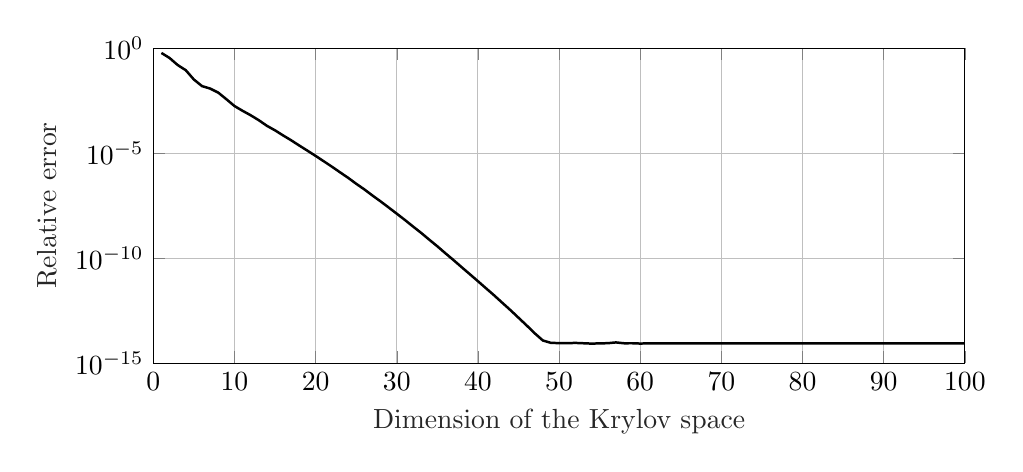
\begin{tikzpicture}

\begin{axis}[%
width=.85\linewidth,
height=4cm,
at={(0in,0in)},
scale only axis,
xmin=0,
xmax=100,
xlabel style={font=\color{white!15!black}},
xlabel={Dimension of the Krylov space},
ymode=log,
ymin=1e-15,
ymax=1,
yminorticks=true,
ylabel style={font=\color{white!15!black}},
ylabel={Relative error},
axis background/.style={fill=white},
xmajorgrids,
ymajorgrids,
yminorgrids,
legend style={legend cell align=left, align=left, draw=white!15!black}
]
\addplot [color=black, line width=0.9pt]
  table[row sep=crcr]{%
1	0.590797345125722\\
2	0.341234080677329\\
3	0.157272930997486\\
4	0.0891400660775228\\
5	0.0320705757210709\\
6	0.0155937592828873\\
7	0.0119253439510956\\
8	0.00763647480225516\\
9	0.00370976324235097\\
10	0.00175449739195379\\
11	0.00103882739089212\\
12	0.000637211140479853\\
13	0.000369644822326709\\
14	0.00020025589215471\\
15	0.00012171128732808\\
16	6.94790567940788e-05\\
17	4.06274966953835e-05\\
18	2.28586221106122e-05\\
19	1.30573267555829e-05\\
20	7.38475979640541e-06\\
21	4.11777447737777e-06\\
22	2.2746904704151e-06\\
23	1.22834302529417e-06\\
24	6.71482740589636e-07\\
25	3.48130942832957e-07\\
26	1.882948292104e-07\\
27	9.62426101173857e-08\\
28	5.06505526015461e-08\\
29	2.58114340082748e-08\\
30	1.30835245506393e-08\\
31	6.57910223892581e-09\\
32	3.21453549599977e-09\\
33	1.59798125349195e-09\\
34	7.57153668307443e-10\\
35	3.66232192610335e-10\\
36	1.69377073233484e-10\\
37	8.01276854328485e-11\\
38	3.69522134517387e-11\\
39	1.72010932723169e-11\\
40	7.96657519147638e-12\\
41	3.65648730747314e-12\\
42	1.68429788109203e-12\\
43	7.48545090813516e-13\\
44	3.35657977698355e-13\\
45	1.44881706755593e-13\\
46	6.25334721934521e-14\\
47	2.63123292955714e-14\\
48	1.1960413249196e-14\\
49	9.20990245321545e-15\\
50	8.98273327994632e-15\\
51	8.90970086473988e-15\\
52	9.16748574882774e-15\\
53	8.82775960859607e-15\\
54	8.49899888132768e-15\\
55	8.70717663222432e-15\\
56	8.89523017820352e-15\\
57	9.6665709467992e-15\\
58	8.82244157379507e-15\\
59	8.84036448276274e-15\\
60	8.54206663471901e-15\\
61	8.73570110668757e-15\\
62	8.73570110668757e-15\\
63	8.73570110668757e-15\\
64	8.73570110668757e-15\\
65	8.73570110668757e-15\\
66	8.73570110668757e-15\\
67	8.73570110668757e-15\\
68	8.73570110668757e-15\\
69	8.73570110668757e-15\\
70	8.73570110668757e-15\\
71	8.73570110668757e-15\\
72	8.73570110668757e-15\\
73	8.73570110668757e-15\\
74	8.73570110668757e-15\\
75	8.73570110668757e-15\\
76	8.73570110668757e-15\\
77	8.73570110668757e-15\\
78	8.73570110668757e-15\\
79	8.73570110668757e-15\\
80	8.73570110668757e-15\\
81	8.73570110668757e-15\\
82	8.73570110668757e-15\\
83	8.73570110668757e-15\\
84	8.73570110668757e-15\\
85	8.73570110668757e-15\\
86	8.73570110668757e-15\\
87	8.73570110668757e-15\\
88	8.73570110668757e-15\\
89	8.73570110668757e-15\\
90	8.73570110668757e-15\\
91	8.73570110668757e-15\\
92	8.73570110668757e-15\\
93	8.73570110668757e-15\\
94	8.73570110668757e-15\\
95	8.73570110668757e-15\\
96	8.73570110668757e-15\\
97	8.73570110668757e-15\\
98	8.73570110668757e-15\\
99	8.73570110668757e-15\\
100	8.73570110668757e-15\\
};
%\addlegendentry{data1}

\end{axis}
\end{tikzpicture}%
        \caption{$\epsilon = 0.05$}
        \label{fig:ode_0.05}
    \end{subfigure}\hspace{.05\linewidth}
    \begin{subfigure}[b]{.45\linewidth}
        % This file was created by matlab2tikz.
%
%The latest updates can be retrieved from
%  http://www.mathworks.com/matlabcentral/fileexchange/22022-matlab2tikz-matlab2tikz
%where you can also make suggestions and rate matlab2tikz.
%
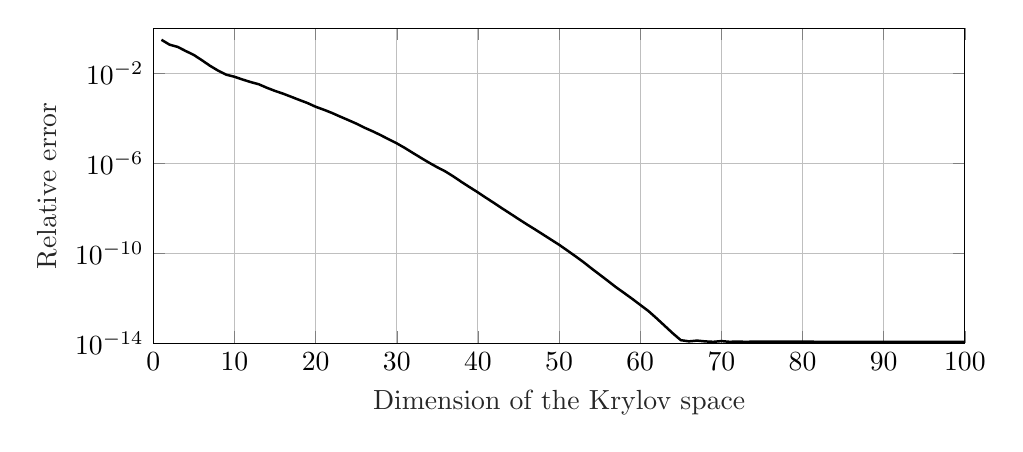
\begin{tikzpicture}

\begin{axis}[%
width=.85\linewidth,
height=4cm,
at={(0in,0in)},
scale only axis,
xmin=0,
xmax=100,
xlabel style={font=\color{white!15!black}},
xlabel={Dimension of the Krylov space},
ymode=log,
ymin=1e-14,
ymax=1,
yminorticks=true,
ylabel style={font=\color{white!15!black}},
ylabel={Relative error},
axis background/.style={fill=white},
xmajorgrids,
ymajorgrids,
yminorgrids,
legend style={legend cell align=left, align=left, draw=white!15!black}
]
\addplot [color=black, line width=0.9pt]
  table[row sep=crcr]{%
1	0.305908729770176\\
2	0.185842348482017\\
3	0.148004926114265\\
4	0.0967602920715717\\
5	0.0648025410697794\\
6	0.0374906795616609\\
7	0.0212681986876963\\
8	0.0129404303440192\\
9	0.00857636695438943\\
10	0.00696983122246\\
11	0.0052436702771879\\
12	0.0040430520213184\\
13	0.00322793629662881\\
14	0.00225043739467314\\
15	0.00163420989998425\\
16	0.0012317053085581\\
17	0.000894599827770048\\
18	0.000646481190339189\\
19	0.000472641931763846\\
20	0.000323747503937065\\
21	0.000239237232699965\\
22	0.000172464606407331\\
23	0.000119267767777074\\
24	8.33546869160878e-05\\
25	5.79065746368e-05\\
26	3.83310896870106e-05\\
27	2.64973950305888e-05\\
28	1.77956353172652e-05\\
29	1.1572385222042e-05\\
30	7.63111644290351e-06\\
31	4.75642097235582e-06\\
32	2.84007682669571e-06\\
33	1.71696918621979e-06\\
34	1.04443317998124e-06\\
35	6.57734489776193e-07\\
36	4.28651820530108e-07\\
37	2.55066150563038e-07\\
38	1.45231230007161e-07\\
39	8.52079339309969e-08\\
40	5.04567246510479e-08\\
41	2.90386860768354e-08\\
42	1.69052039752362e-08\\
43	9.73916094512884e-09\\
44	5.70287754878932e-09\\
45	3.31176300104464e-09\\
46	1.94267818061846e-09\\
47	1.16221732506671e-09\\
48	6.86205349497406e-10\\
49	4.0331986801663e-10\\
50	2.3777682784408e-10\\
51	1.33195796008228e-10\\
52	7.38789284933916e-11\\
53	4.03691572879177e-11\\
54	2.09532560448374e-11\\
55	1.11688818330872e-11\\
56	5.9290452312746e-12\\
57	3.10778224572015e-12\\
58	1.72293872958609e-12\\
59	9.430732382795e-13\\
60	5.05177562527383e-13\\
61	2.70453670846753e-13\\
62	1.29267808561687e-13\\
63	5.99638388081284e-14\\
64	2.77124868607469e-14\\
65	1.36416588675984e-14\\
66	1.20608922532971e-14\\
67	1.30538908154694e-14\\
68	1.20204110642728e-14\\
69	1.15053833173926e-14\\
70	1.23939147588686e-14\\
71	1.15288488594861e-14\\
72	1.17708949199402e-14\\
73	1.15099822915781e-14\\
74	1.17115726182429e-14\\
75	1.16095322259592e-14\\
76	1.17422209767356e-14\\
77	1.18564037625219e-14\\
78	1.16831660905169e-14\\
79	1.18867501777877e-14\\
80	1.17585807800807e-14\\
81	1.1734565908154e-14\\
82	1.14063627929465e-14\\
83	1.14063627929465e-14\\
84	1.14063627929465e-14\\
85	1.14063627929465e-14\\
86	1.14063627929465e-14\\
87	1.14063627929465e-14\\
88	1.14063627929465e-14\\
89	1.14063627929465e-14\\
90	1.14063627929465e-14\\
91	1.14063627929465e-14\\
92	1.14063627929465e-14\\
93	1.14063627929465e-14\\
94	1.14063627929465e-14\\
95	1.14063627929465e-14\\
96	1.14063627929465e-14\\
97	1.14063627929465e-14\\
98	1.14063627929465e-14\\
99	1.14063627929465e-14\\
100	1.14063627929465e-14\\
};
%\addlegendentry{data1}

\end{axis}
\end{tikzpicture}%
        \caption{$\epsilon = 0.1$}
        \label{fig:ode_0.1}
    \end{subfigure}
    \caption{Convergence of our algorithm for different diffusivity value $\epsilon$. We note that as the dissufivity increases, the need to work in higher dimension increases too, thus slowing down the convergence of our algorithm. This suggests that diffusivity impacts the conditioning of $\mathbf{A}$.}
    \label{fig:ode_eps}
\end{figure}

\begin{figure}
    \centering
    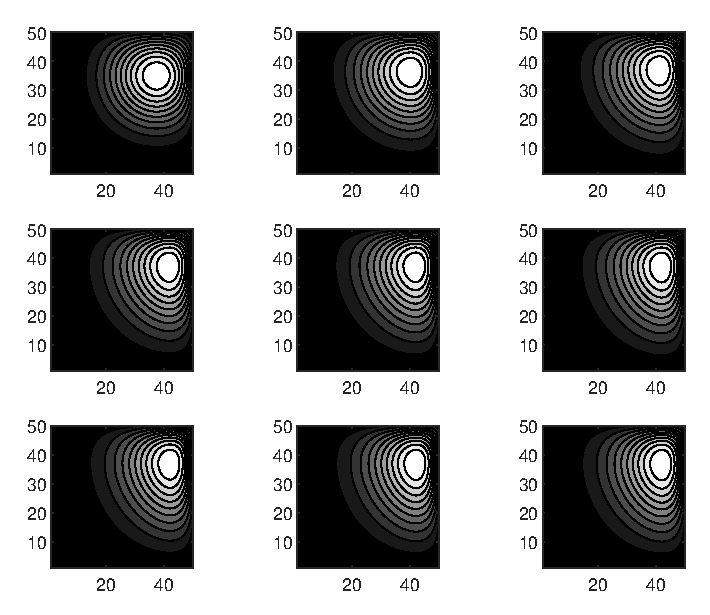
\includegraphics[width=.7\linewidth]{figures/convection_krylov.pdf}
    \caption{Result of solving the convection-diffusion equation with our method. For the sake of conciseness, we are not showing results from the exact solution as they are humanly undistinguishable.}
\end{figure}

\subsection{The sign function}\label{sec:sign}
\subsubsection{Background and theory}
In control theory we are often interested in the eigenvalues $\lambda$ of system matrices with $Re(\lambda)>0$, since they correspond to unstable poles. In the design of controllers it is therefore interesting to have an efficient way to count the number of eigenvalues of a matrix in the right half-plane $Re(z)>0$. Here we will build such a method.
\begin{theorem}\label{thm:sign}
Let $\mathbf{A}\in\mathbb{C}^{n \times n}$ be a matrix with $k_{-}$ eigenvalues in the left plane, $k_{+}$ eigenvalues in the right plane and none on the imaginary axis, counting multiplicity. Let $\text{sgn}:\mathbb{C}\mapsto \{1,-1\}$ be defined by
$$\text{sgn}(z)= \begin{cases} 
      1 & Re(z)\geq 0 \\
      -1 & Re(z)<0. 
   \end{cases}
$$
Then $\text{trace}(\text{sgn}(\mathbf{A}))=k_{+}-k_{-}$.
\end{theorem}
\begin{proof}
    Let $\mathbf{A}\in\mathbb{C}^{n\times n}$. To stay in a very general scenario, and consider cases where $\mathbf{A}$, let us consider its Jordan Canonical Form :
    \begin{equation*}
        \mathbf{A} = \mathbf{VJV}^{-1}
    \end{equation*} 
    Recall that by theorem \ref{thm:jordan}, consider $f$ a function, then 
    \begin{equation*}
        f(\mathbf{A}) = \mathbf{V}f(\mathbf{J})\mathbf{V}^{-1}
    \end{equation*}
    Thus let us consider the decomposition where 
    \begin{equation*}
        \mathbf{J} = \begin{pmatrix}
            \mathbf{J}_{k_+} & 0 \\ 0 & \mathbf{J}_{k_-}
        \end{pmatrix}
    \end{equation*}
    such that $\mathbf{J}_{k_+}$ has $k_+$ eigenvalues in the right plane, and $\mathbf{J}_{k_-}$ has $k_-$ eigenvalues in the left plane. Then, we have that
    \begin{equation*}
        \text{sgn}(\mathbf{J}) = \begin{pmatrix}
            \mathbf{I}_{k_+} & 0 \\ 0 & -\mathbf{I}_{k_-}
        \end{pmatrix}
    \end{equation*}
    where $\mathbf{I}_n$ is the identity matrix of size $n$. Then, we have that
    \begin{equation*}
        \text{trace}(\text{sgn}(\mathbf{J})) = k_+ - k_-
    \end{equation*}
    And thus, we have that
    \begin{equation*}
        \text{trace}(\text{sgn}(\mathbf{A})) = \text{trace}(\text{sgn}(\mathbf{VJV}^{-1})) = \mathbf{V}\text{trace}(\text{sgn}(\mathbf{J}))\mathbf{V}^{-1} = (k_+-k_-)\mathbf{V}\mathbf{V}^{-1} = k_+ - k_-
    \end{equation*}
\end{proof}
\subsubsection{Stability of a system}
In this section, we will see how theorem \ref{thm:sign} is a powerful tool for system stability assessment. Let us consider a system modeled by the matrix $\mathbf{A}\in\mathbb{C}^{n\times n}$, large and sparse. Say it has $p$ distinct eigenvalues $\lambda_i$, $i=1,\dots,p$. We know that if $\forall i, Re(\lambda_i)<0$, then the system is stable. Using the sign function, it immediately rewrites, if $\forall i, sign(Re(\lambda_i)) = -1$ then the system is stable. From theorem \ref{thm:sign}, we can design an algorithm that counts positive eigenvalues of a system. Obviously, when $n$ is extremely large, computing eigenvalues directly on $\mathbf{A}$ is not an option. Algorithm 3 takes advantage of the properties of Arnoldi method and estimates via Monte-Carlo sampling the number of positive eigenvalues of $\mathbf{A}$.

\begin{algorithm2e}
    \SetAlgoLined
    \KwData{$A \in \mathbb{C}^{n \times n}$, $k \in \mathbb{N}$, $N \in \mathbb{N}$}
    \KwResult{$k_+ \in \mathbb{R}$}
    \caption{Computing $k_{+}(A)$}
    $\mathbf{q} \gets \mathbf{0}\in\mathbb{R}^{N}$\;
    \For{$i = 1$ \KwTo $N$}{
      $\mathbf{u} \gets \text{randn}(n, 1)$\;
      $\hat{\mathbf{u}} \gets \frac{\mathbf{u}}{\|\mathbf{u}\|}$\;
      $[H, Q] \gets \text{arnoldi}(A, \hat{\mathbf{u}}, k)$\;
      $q(i) \gets \text{trace}(\text{sign}(H)))$\;
    }
    $q_+ := \text{mode}(\mathbf{q}) $\;
    $k_+\gets (q+k)/2$
\end{algorithm2e}
\subsubsection{Limitation of simple Arnoldi Method}
In the previous algorithm to compute positive eigenvalues, we assume the function \texttt{arnoldi()} is the Matlab's translation of Algorithm 1, \textit{i.e} Modified Gram-Schmidt Arnoldi method. In this section we will see that the convergence of Arnoldi Method is actually not guaranteed in a reasonable time for all systems. The efficiency of the Arnoldi algorithm is highly correlated to the condition number of the matrix $\mathbf{A}$. We know from experience, that Ritz Value struggle to converge properly where eigenvalues of the matrix are very close to each other.

Provided with this note, a matrix that has those properties. Using Matlab's \texttt{eigs} function, we observe that the eigenvalues of $\mathbf{A}$ are clustered and very close to each other (figure \ref{fig:ritz_poor_cond}). This leads ultimately to very slow convergence of the eigenvalues using Arnolid method (figure \ref{fig:sign_difficult_est}). 
\begin{figure}
    \centering
    \begin{subfigure}[b]{.45\linewidth}
        % This file was created by matlab2tikz.
%
%The latest updates can be retrieved from
%  http://www.mathworks.com/matlabcentral/fileexchange/22022-matlab2tikz-matlab2tikz
%where you can also make suggestions and rate matlab2tikz.
%
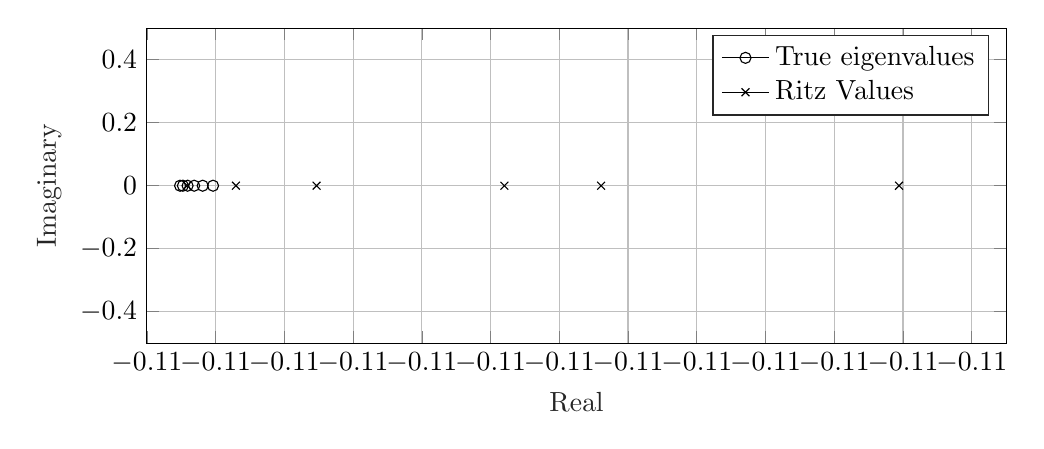
\begin{tikzpicture}

\begin{axis}[%
width=.9\linewidth,
height=4cm,
at={(0in,0in)},
scale only axis,
xmin=-0.1114,
xmax=-0.11115,
xlabel style={font=\color{white!15!black}},
xlabel={Real},
ymin=-0.5,
ymax=0.5,
ylabel style={font=\color{white!15!black}},
ylabel={Imaginary},
axis background/.style={fill=white},
xmajorgrids,
ymajorgrids,
legend style={legend cell align=left, align=left, draw=white!15!black}
]
\addplot [color=black, draw=none, mark=o, mark options={solid, black}]
  table[row sep=crcr]{%
-0.111390339495116	0\\
-0.111389516591765	0\\
-0.111388145095192	0\\
-0.111386225018897	0\\
-0.111383756381798	0\\
-0.11138073920822	0\\
};
\addlegendentry{True eigenvalues}

\addplot [color=black, draw=none, mark=x, mark options={solid, black}]
  table[row sep=crcr]{%
-0.111388247730224	0\\
-0.111374081198001	0\\
-0.111350623743485	0\\
-0.111295975748161	0\\
-0.111267844878066	0\\
-0.111181160089968	0\\
};
\addlegendentry{Ritz Values}

\end{axis}
\end{tikzpicture}%
        \caption{}
        \label{fig:ritz_poor_cond}
    \end{subfigure}\hspace{0.05\linewidth}
    \begin{subfigure}[b]{.45\linewidth}
        % This file was created by matlab2tikz.
%
%The latest updates can be retrieved from
%  http://www.mathworks.com/matlabcentral/fileexchange/22022-matlab2tikz-matlab2tikz
%where you can also make suggestions and rate matlab2tikz.
%
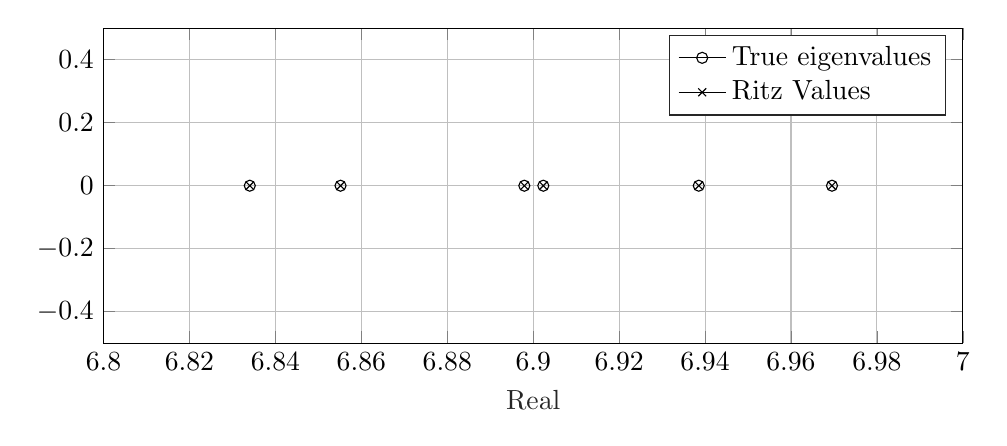
\begin{tikzpicture}

\begin{axis}[%
width=.9\linewidth,
height=4cm,
at={(0in,0in)},
scale only axis,
xmin=6.8,
xmax=7,
xlabel style={font=\color{white!15!black}},
xlabel={Real},
ymin=-0.5,
ymax=0.5,
ylabel style={font=\color{white!15!black}},
%ylabel={Imaginary},
axis background/.style={fill=white},
xmajorgrids,
ymajorgrids,
legend style={legend cell align=left, align=left, draw=white!15!black}
]
\addplot [color=black, draw=none, mark=o, mark options={solid, black}]
  table[row sep=crcr]{%
6.96954408283504	0\\
6.93853500100255	0\\
6.90235495542524	0\\
6.89793392988137	0\\
6.85515514528339	0\\
6.8340301735165	0\\
};
\addlegendentry{True eigenvalues}

\addplot [color=black, draw=none, mark=x, mark options={solid, black}]
  table[row sep=crcr]{%
6.96954408283502	0\\
6.93853500100252	0\\
6.90235495542526	0\\
6.89793392988139	0\\
6.85515514528345	0\\
6.83403017351649	0\\
};
\addlegendentry{Ritz Values}

\end{axis}

\end{tikzpicture}%
        \caption{}
        \label{fig:ritz_good_cond}
    \end{subfigure}
    \begin{subfigure}[b]{.45\linewidth}
        % This file was created by matlab2tikz.
%
%The latest updates can be retrieved from
%  http://www.mathworks.com/matlabcentral/fileexchange/22022-matlab2tikz-matlab2tikz
%where you can also make suggestions and rate matlab2tikz.
%
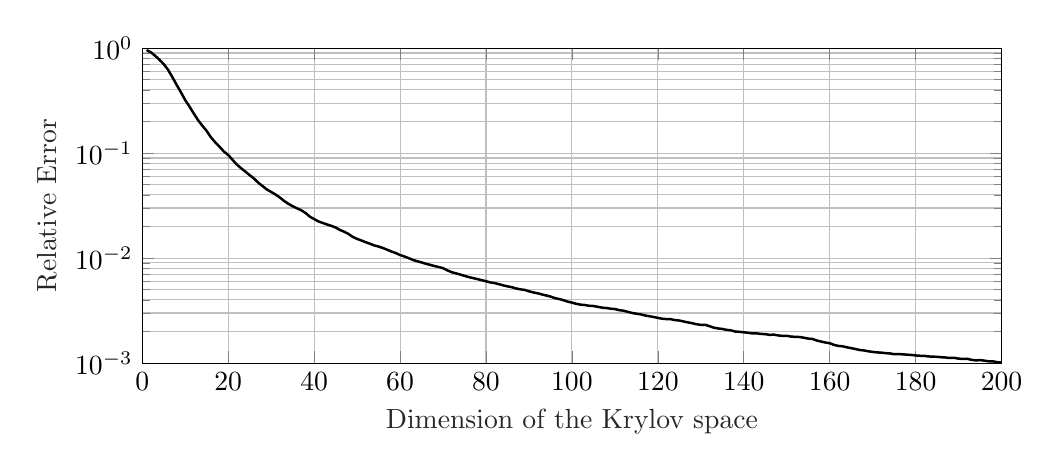
\begin{tikzpicture}

\begin{axis}[%
width=.9\linewidth,
height=4cm,
at={(0in,0in)},
scale only axis,
xmin=0,
xmax=200,
xlabel style={font=\color{white!15!black}},
xlabel={Dimension of the Krylov space},
ymode=log,
ymin=0.001,
ymax=1,
yminorticks=true,
ylabel style={font=\color{white!15!black}},
ylabel={Relative Error},
axis background/.style={fill=white},
xmajorgrids,
ymajorgrids,
yminorgrids,
legend style={legend cell align=left, align=left, draw=white!15!black}
]
\addplot [color=black, line width=0.9pt]
  table[row sep=crcr]{%
1	0.958159223208536\\
2	0.912732322692792\\
3	0.845534567574491\\
4	0.77656258361038\\
5	0.704046935611853\\
6	0.622338959653795\\
7	0.530046288233711\\
8	0.447338052414807\\
9	0.379785731422014\\
10	0.32001122337058\\
11	0.277132808628033\\
12	0.238057013663392\\
13	0.205843841681723\\
14	0.182012266617629\\
15	0.162675310281711\\
16	0.141148143800187\\
17	0.126472434670345\\
18	0.114920268375819\\
19	0.103619321138117\\
20	0.0959987976649167\\
21	0.0864827181714266\\
22	0.0778313301489386\\
23	0.0719411821191096\\
24	0.0666752904642562\\
25	0.0617530309446763\\
26	0.0573692215883609\\
27	0.0522337507304662\\
28	0.0485751126058312\\
29	0.0450443027449175\\
30	0.0427367548350678\\
31	0.0403987439128814\\
32	0.0378634619735729\\
33	0.035116721613039\\
34	0.0329425964770057\\
35	0.0312315443313319\\
36	0.0298587917315737\\
37	0.0285427759560372\\
38	0.0269391111928132\\
39	0.0248394664114489\\
40	0.0235641640696687\\
41	0.0223763633323984\\
42	0.0216290336553107\\
43	0.0209185432388349\\
44	0.0202923726347032\\
45	0.0195971385188271\\
46	0.0185603962421279\\
47	0.0178501541247304\\
48	0.0169849631446645\\
49	0.0159270034270842\\
50	0.0152475591813519\\
51	0.0147311208447153\\
52	0.0141889511496243\\
53	0.0137132023635383\\
54	0.0132152197869626\\
55	0.0128943091532633\\
56	0.0124925360425475\\
57	0.0120293578281277\\
58	0.0115597806713754\\
59	0.0111825238407229\\
60	0.0107035576842279\\
61	0.0103727924698745\\
62	0.00999796097277805\\
63	0.0096225948165427\\
64	0.00933813300520287\\
65	0.00910309495930928\\
66	0.00884389139286572\\
67	0.00863356730189845\\
68	0.00841112687654379\\
69	0.00822842423866423\\
70	0.00802057368348649\\
71	0.00765417824524155\\
72	0.00734704830453321\\
73	0.00716752395491411\\
74	0.00697990710144119\\
75	0.00677949760138124\\
76	0.00660179346097439\\
77	0.00645832551650925\\
78	0.00631265367586724\\
79	0.00616741223819168\\
80	0.0060298343029999\\
81	0.00586997791657267\\
82	0.00578876520358035\\
83	0.00565383325795095\\
84	0.00550752610769233\\
85	0.00538615175934895\\
86	0.00529090384804518\\
87	0.00514071704429413\\
88	0.0050459925240797\\
89	0.00498276967467164\\
90	0.00483477366281887\\
91	0.00471588300650521\\
92	0.0046312066108988\\
93	0.00451355137097895\\
94	0.00441276265789274\\
95	0.00431023781414175\\
96	0.00416375884812718\\
97	0.00408025525226829\\
98	0.0039826396557351\\
99	0.00385397628349854\\
100	0.00377421366354697\\
101	0.00367330885849805\\
102	0.00360547758646219\\
103	0.00357677530350359\\
104	0.00351948348529572\\
105	0.00349885843056822\\
106	0.00344165299366735\\
107	0.00337604238847402\\
108	0.00334928039051712\\
109	0.00330140981659798\\
110	0.00327502076866001\\
111	0.0031964742943956\\
112	0.00315727750749874\\
113	0.00308089328198903\\
114	0.00300538636314117\\
115	0.00295628870613568\\
116	0.00291535809827201\\
117	0.00284587007988221\\
118	0.00279905472589403\\
119	0.00275130011972031\\
120	0.00269699497975659\\
121	0.00264968909383933\\
122	0.00262880371658646\\
123	0.00261991652969697\\
124	0.00257005944567095\\
125	0.00254615087965291\\
126	0.00249274852498048\\
127	0.00244333957108684\\
128	0.00240004647902137\\
129	0.00234677255785212\\
130	0.00231482909633731\\
131	0.00231767958686065\\
132	0.00225221591194288\\
133	0.00217887092402182\\
134	0.00214001137871005\\
135	0.00211633944087209\\
136	0.00207426379759466\\
137	0.0020537697441093\\
138	0.00200011868756599\\
139	0.00198772691940536\\
140	0.00196710793785205\\
141	0.00194480826829107\\
142	0.00191949526131612\\
143	0.00191969358473577\\
144	0.00189873472280232\\
145	0.00188721082119017\\
146	0.00185992730625803\\
147	0.00186731348709827\\
148	0.0018370282405697\\
149	0.00181696644325072\\
150	0.00182188677488205\\
151	0.00178927053491824\\
152	0.00177935462553335\\
153	0.0017727983319799\\
154	0.00174607039536936\\
155	0.00171291605524999\\
156	0.00169959076956192\\
157	0.00164259214257262\\
158	0.00160507798183862\\
159	0.00157168553285651\\
160	0.00154812295827096\\
161	0.00149262892655291\\
162	0.00145904704529622\\
163	0.00144710488338944\\
164	0.00141423513826282\\
165	0.00139006578361633\\
166	0.00136216300504011\\
167	0.00133293377481243\\
168	0.00132106303792881\\
169	0.00129637624454102\\
170	0.00127865617863957\\
171	0.00126554101945333\\
172	0.00125895921322586\\
173	0.00124493236902892\\
174	0.00123683380980776\\
175	0.0012175095949984\\
176	0.00121999146442754\\
177	0.00121285936697612\\
178	0.00120419010452214\\
179	0.00119636912075355\\
180	0.0011834984744819\\
181	0.00117571851247015\\
182	0.00117213155389733\\
183	0.00115818761830609\\
184	0.00115114521619874\\
185	0.00114957408415345\\
186	0.0011377251423337\\
187	0.00113074491993127\\
188	0.00111902534318155\\
189	0.00112262247181771\\
190	0.00110355183692462\\
191	0.00109749622872261\\
192	0.00110081414247497\\
193	0.00107471232025927\\
194	0.00106113486521265\\
195	0.00106855494513568\\
196	0.00105608154578947\\
197	0.00104079121633438\\
198	0.00104005540316842\\
199	0.00102064393791568\\
200	0.00101495153058911\\
};
%\addlegendentry{data1}

\end{axis}
\end{tikzpicture}%
        \caption{}
        \label{fig:sign_difficult_est}
    \end{subfigure}\hspace{0.05\linewidth}
    \begin{subfigure}[b]{.45\linewidth}
        % This file was created by matlab2tikz.
%
%The latest updates can be retrieved from
%  http://www.mathworks.com/matlabcentral/fileexchange/22022-matlab2tikz-matlab2tikz
%where you can also make suggestions and rate matlab2tikz.
%
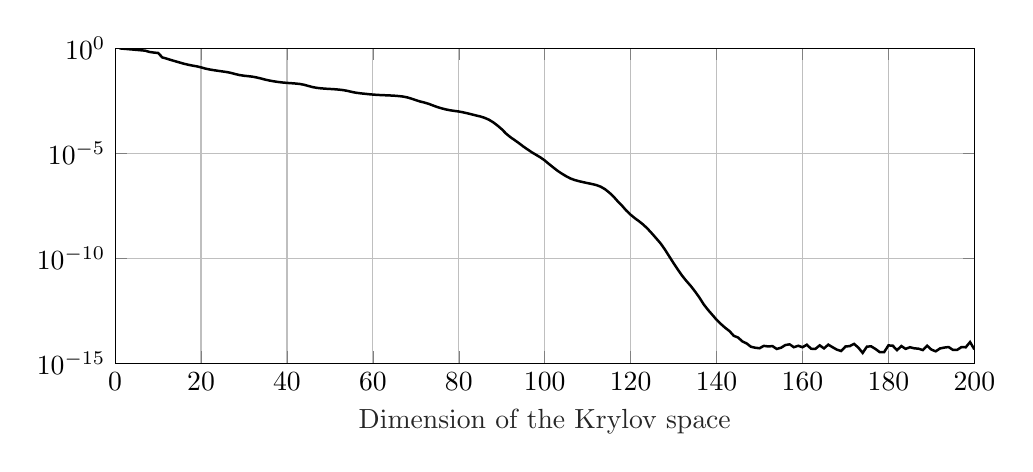
\begin{tikzpicture}

\begin{axis}[%
width=.9\linewidth,
height=4cm,
at={(0in,0in)},
scale only axis,
xmin=0,
xmax=200,
xlabel style={font=\color{white!15!black}},
xlabel={Dimension of the Krylov space},
ymode=log,
ymin=1e-15,
ymax=1,
yminorticks=true,
ylabel style={font=\color{white!15!black}},
%ylabel={Relative Error},
axis background/.style={fill=white},
xmajorgrids,
ymajorgrids,
yminorgrids,
legend style={legend cell align=left, align=left, draw=white!15!black}
]
\addplot [color=black, line width=0.9pt]
  table[row sep=crcr]{%
1	0.975745933012263\\
2	0.937820365710568\\
3	0.899743731932046\\
4	0.864547305859143\\
5	0.828697724903052\\
6	0.793497723978064\\
7	0.760740967677957\\
8	0.660862364380392\\
9	0.616983403162241\\
10	0.590257847102173\\
11	0.362588326885871\\
12	0.317075399909951\\
13	0.273736603043343\\
14	0.238432625884944\\
15	0.207922192586271\\
16	0.18181930397035\\
17	0.162767662492028\\
18	0.148036070600711\\
19	0.136360101637585\\
20	0.121516686813063\\
21	0.106732367844731\\
22	0.0965763379419131\\
23	0.0892184855908525\\
24	0.083222987791517\\
25	0.0778272671860687\\
26	0.0726595581080044\\
27	0.0661110399244452\\
28	0.0582617518485937\\
29	0.0522416292088067\\
30	0.0486857079769039\\
31	0.0463376514049361\\
32	0.0437609639786903\\
33	0.0399844236662653\\
34	0.035704439782971\\
35	0.0315044716111673\\
36	0.0285360166087997\\
37	0.0262022379784772\\
38	0.0244750961122216\\
39	0.0231470114204541\\
40	0.0221492009874116\\
41	0.0214439285433954\\
42	0.0206937815051394\\
43	0.0196888409026906\\
44	0.0180207566854541\\
45	0.0157911926632353\\
46	0.0139720440275594\\
47	0.0128325501612904\\
48	0.0121659551590386\\
49	0.0117322641903737\\
50	0.0114165123262216\\
51	0.0110823428228737\\
52	0.0106686512654739\\
53	0.0101020019692223\\
54	0.00931101207791422\\
55	0.00834064327556069\\
56	0.00759188395406558\\
57	0.00710930064050349\\
58	0.00676323817820266\\
59	0.00644380236239689\\
60	0.00616155316175262\\
61	0.00595403956535862\\
62	0.00581294427546677\\
63	0.00570195193250138\\
64	0.00558502582458092\\
65	0.00543495768979139\\
66	0.00523768195151951\\
67	0.00495660500055943\\
68	0.00452615105979966\\
69	0.00393351775706033\\
70	0.00334717204985722\\
71	0.00288119650553439\\
72	0.00256269126377563\\
73	0.00222947005423041\\
74	0.00186119798671113\\
75	0.00156805236923813\\
76	0.00135903334330801\\
77	0.00120502490778097\\
78	0.00110069666705378\\
79	0.00102512314550274\\
80	0.000961346803310167\\
81	0.00087855818296802\\
82	0.000789941275115594\\
83	0.000702248003953977\\
84	0.000623615072295749\\
85	0.00055954045557404\\
86	0.00048120065136586\\
87	0.000393047895549532\\
88	0.00029458557569526\\
89	0.000207087668247718\\
90	0.000137821616275722\\
91	8.54481401618264e-05\\
92	5.78885640482841e-05\\
93	4.18744824947173e-05\\
94	2.98943544566844e-05\\
95	2.08483786804652e-05\\
96	1.50461534674511e-05\\
97	1.0954752050358e-05\\
98	8.28702934745645e-06\\
99	6.25957373130175e-06\\
100	4.49286337049649e-06\\
101	3.02603735470511e-06\\
102	2.07519507165944e-06\\
103	1.43823102115687e-06\\
104	1.05099228110948e-06\\
105	7.91348084813724e-07\\
106	6.20201836526884e-07\\
107	5.21745679966488e-07\\
108	4.61165699100128e-07\\
109	4.11855694670341e-07\\
110	3.73195396623196e-07\\
111	3.38226098259781e-07\\
112	3.02396144696559e-07\\
113	2.53902486761272e-07\\
114	1.93701717085213e-07\\
115	1.33858413667149e-07\\
116	8.59840186750108e-08\\
117	5.05715635034267e-08\\
118	3.12526500946821e-08\\
119	1.83279635605616e-08\\
120	1.16538196347445e-08\\
121	7.93102219074877e-09\\
122	5.6108369398199e-09\\
123	3.84469792174909e-09\\
124	2.44227118328891e-09\\
125	1.45833347758793e-09\\
126	8.54006214814452e-10\\
127	4.93744159908735e-10\\
128	2.52586223614258e-10\\
129	1.19486599849041e-10\\
130	5.72392493670296e-11\\
131	2.82078132014205e-11\\
132	1.43739355590797e-11\\
133	8.05901920487498e-12\\
134	4.69881569372109e-12\\
135	2.56161980246802e-12\\
136	1.32480604772939e-12\\
137	6.30172197134291e-13\\
138	3.44074338589877e-13\\
139	2.0020262008974e-13\\
140	1.15882972981153e-13\\
141	7.34031314834739e-14\\
142	4.81316009650352e-14\\
143	3.36111547030828e-14\\
144	1.99897689819818e-14\\
145	1.65484601131169e-14\\
146	1.087451204372e-14\\
147	8.64385078385829e-15\\
148	6.01166783475526e-15\\
149	5.40624740567619e-15\\
150	5.10893526644252e-15\\
151	6.64469430774971e-15\\
152	6.22339647989504e-15\\
153	6.46585213660436e-15\\
154	4.72999666387331e-15\\
155	5.40445916076774e-15\\
156	7.2552597666178e-15\\
157	7.85142238919162e-15\\
158	5.72819793358309e-15\\
159	6.69417796881223e-15\\
160	5.7272335904898e-15\\
161	7.49786712024777e-15\\
162	4.8390915214385e-15\\
163	4.76982463357227e-15\\
164	7.03003309769501e-15\\
165	5.02829434825065e-15\\
166	7.57208800053373e-15\\
167	5.70428252728592e-15\\
168	4.38299832822141e-15\\
169	3.76767191488031e-15\\
170	6.18846267822914e-15\\
171	6.46157945250821e-15\\
172	8.23143776158853e-15\\
173	5.47427234904645e-15\\
174	3.05301126613033e-15\\
175	6.13805168331888e-15\\
176	6.25725260844039e-15\\
177	4.68570650633649e-15\\
178	3.304949001181e-15\\
179	3.35800399360659e-15\\
180	6.99123038283267e-15\\
181	6.74964361291917e-15\\
182	4.14597148055878e-15\\
183	6.52452944856003e-15\\
184	4.78745164682266e-15\\
185	5.70161906776087e-15\\
186	5.08074782228515e-15\\
187	4.87094670556399e-15\\
188	4.17021422136222e-15\\
189	6.76435764092184e-15\\
190	4.40499673722165e-15\\
191	3.64320325737572e-15\\
192	4.99909986362236e-15\\
193	5.49717893416239e-15\\
194	5.83022428519951e-15\\
195	4.29387781687192e-15\\
196	4.27518487264538e-15\\
197	5.82026821288204e-15\\
198	5.6727253368459e-15\\
199	1.00714072651201e-14\\
200	4.51338075101602e-15\\
};
%\addlegendentry{data1}

\end{axis}
\end{tikzpicture}%
        \caption{}
        \label{fig:sign_easy_est}
    \end{subfigure}
    \caption{Comparison of the convergence of Arnoldi method to two different matrices. The first matrix (figures \ref{fig:ritz_poor_cond} and \ref{fig:sign_difficult_est}) is from section \ref{sec:sign}. We see from figure \ref{fig:ritz_poor_cond} that the eigenvalues are clustered and very close to each other, leading to poor convergences of the Ritz values. We see that even after 200 iterations, the method is far from having converged. On the other end of the spectrum, when applied to the matrix we have studied earlier in the matrix-vector product, which is better conditioned (figures \ref{fig:ritz_good_cond} and \ref{fig:sign_easy_est}), here, the eigenvalues are well spread, and the Ritz values converge quickly. We see that after 200 iterations, the Ritz values perfectly match the eigenvalues. Figures \ref{fig:sign_difficult_est} and \ref{fig:sign_easy_est} show the relative error in the estimation of the eigenvalues. And indeed we see that for the first matrix, the relative error is still very high after 200 iterations, whereas for the second matrix, the relative error is equal to machine precision from 150 iterations.}
    \label{fig:fullritz}
\end{figure}

From this observation, we can easily say that with our previous implementation of Arnoldi, it seems unsafe to use Algorithm 3 as a tool to estimate the number of positive eigenvalues. We need to find a way to replace line 5 of Algorithm 3 by a more robust method.

\subsubsection{Shifted-Invert Arnoldi Method}
The Shifted-Invert Arnoldi method is a technique that allows for better convergence on ill-conditioned system, given we know some information on the spectrum of $\mathbf{A}$. The whole idea is to combine two ideas that are common to Power Iterations (\cite{saad2011numerical}), namely Shifted Power and Inverted iteration. The idea is fairly simple, instead of applying Arnoldi iterations on $\mathbf{A}$, you will apply it to $(\mathbf{A}-\sigma\mathbf{I})^{-1}$ where $\sigma$ is a shift.

The interesting property about the shift is that it alters the eigenvalues but not the eigenvectors (\cite{saad2011numerical}). Once the eigenvalues $\mu$ of $(\mathbf{A}-\sigma\mathbf{I})^{-1}$ are computed, we can easily recover the eigenvalues of $\mathbf{A}$ by applying the shift $\sigma$ and inverting them
\begin{equation*}
    \lambda_i = \frac{1}{\mu_i} + \sigma
\end{equation*}
\begin{theorem}
    Say you chose an arbitrary $\sigma$, then given $\lambda_i$ and $\lambda_j$ two eigenvalues of $\mathbf{A}$ such that $\forall k \neq i,j$, $\|\sigma-\lambda_k\| > \|\sigma-\lambda_i,j\|$, then the convergence factor of Shifted-Invert method is given by 
    \begin{equation}
        \rho_{\mathbf{I}} = \frac{|\sigma-\lambda_i|}{|\sigma-\lambda_j|}
    \end{equation}
\end{theorem}
Consequently, we see that a good initialization of $\sigma$ is crucial to the convergence of the method. On the other end, a poor choice could have bad effects on the convergence, ultimately not converging at all. Several choices are open to us as for initilization of $\sigma$. One could stick with the unity, proceed to some power iterations, using the trace, or even use the Ritz values as computed in figure \ref{fig:ritz_poor_cond}. Inspired by the convergence rate of Power Iteration that is driven by the ratio of the two largest egeinvalues (in terms of magnitude), I suggest the following $\sigma$ as a good estimator:
\begin{equation}
    \sigma = \mathbb{E}\left[\frac{\lambda_1+\lambda_2}{2}\right]
\end{equation}
where $\lambda_1$ and $\lambda_2$ are the two largest eigenvalues of $\mathbf{A}$ in terms of magnitude. Computationally speaking, the Shifted-Invert procedure looks very heavy, especially considering the inverse operator : inverting such a large matrix is very costly. The good news is that we can take the LU factorization of $(\mathbf{A}-\sigma\mathbf{I})$, and the solve two linear system to compute the inverse. This is much more efficient than inverting the matrix directly. The Shifted-Invert Arnoldi method is described in Algorithm 4.
\begin{algorithm2e}
    \SetAlgoLined
    \KwData{$A \in \mathbb{C}^{n \times n}$, $v_1 \in \mathbb{C}^n$ a unit vector in the chosen norm, $\sigma\in\mathbb{C}$}
    \KwResult{$H_n \in \mathbb{C}^{n\times n}$}
    \caption{Shifted-Invert Arnoldi Iteration}
    $[L,U] \gets \text{lu}(A-\sigma I)$\;
    \For{$k = 1 \KwTo n$}{
        $\mathbf{w} \gets U^{-1}L^{-1}\mathbf{v}_k$\;
        \For{$i = 1 \KwTo k$}{
            $h_{ik} \gets \mathbf{v}_i^*\mathbf{w}$\;
            $\mathbf{w} \gets \mathbf{w} - h_{ik}\mathbf{v}_i$\;
        }
        $h_{k+1,k} \gets \|\mathbf{w}\|$\;
        \If{$h_{k+1,k} = 0$}{
            \textbf{break}\;
        }
        $\mathbf{v_{k+1}} \gets \mathbf{w}/h_{k+1,k}$
    }
    %\label{alg:arnoldi}
    %\label{alg:arnoldi}
\end{algorithm2e}
Note that in algorithm 4, $\sigma$ is not recomputed throughout the iterations. One way to potentially fasten the convergence, or to avoid having to define a good $\sigma$ initially (which can be costly) is to recompute $\sigma$ at each iteration (or at each $i$ iteration). A drawback obviously is that it requires to recompute the LU factorization, which is arguabely the most costly operation in Algorithm 4. We will not investigate this further in this report, but it is worth noting that this could be a potential improvement to the algorithm.

If we take a look at the convergence of the Ritz Values, similarly as in figure \ref{fig:fullritz}, we note that with this method, Ritz values converges no matter the matrix (figure \ref{fig:shiftritz_full}), and in much fewer iterations. We note that the final relative error is slightly higher than the machine precision $\epsilon$, and thus is slightly higher than in the regular Arnoldi Method, maybe because there is a numerical bias introduced by the shift and inverse steps. However, the relative error remains very small, around $10^{-14}$.

\begin{figure}
    \centering
    \begin{subfigure}[b]{.45\linewidth}
        % This file was created by matlab2tikz.
%
%The latest updates can be retrieved from
%  http://www.mathworks.com/matlabcentral/fileexchange/22022-matlab2tikz-matlab2tikz
%where you can also make suggestions and rate matlab2tikz.
%
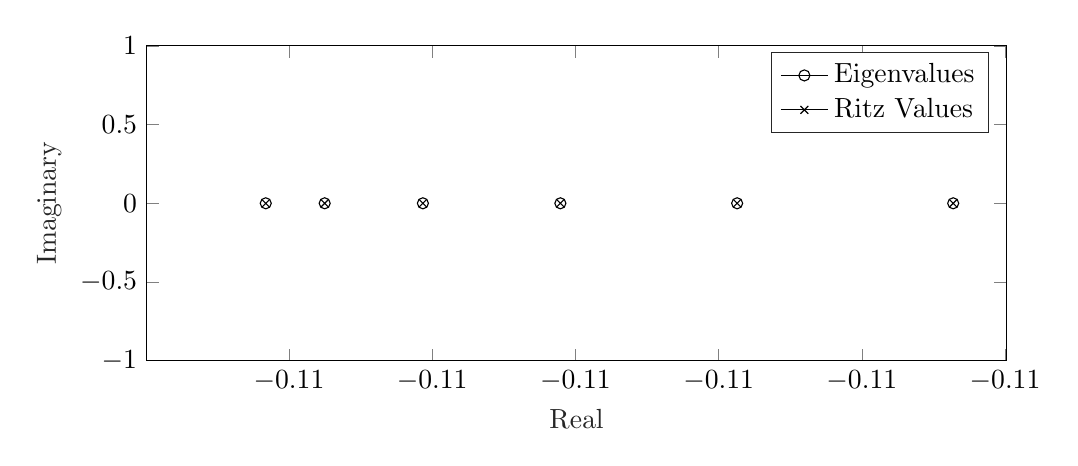
\begin{tikzpicture}

\begin{axis}[%
width=.9\linewidth,
height=4cm,
at={(0in,0in)},
scale only axis,
xmin=-0.111392,
xmax=-0.11138,
xlabel style={font=\color{white!15!black}},
xlabel={Real},
ymin=-1,
ymax=1,
ylabel style={font=\color{white!15!black}},
ylabel={Imaginary},
axis background/.style={fill=white},
legend style={legend cell align=left, align=left, draw=white!15!black}
]
\addplot [color=black, draw=none, mark=o, mark options={solid, black}]
  table[row sep=crcr]{%
-0.111390339495116	0\\
-0.111389516591765	0\\
-0.111388145095192	0\\
-0.111386225018897	0\\
-0.111383756381798	0\\
-0.11138073920822	0\\
};
\addlegendentry{Eigenvalues}

\addplot [color=black, draw=none, mark=x, mark options={solid, black}]
  table[row sep=crcr]{%
-0.111390339495114	0\\
-0.111389516591765	0\\
-0.111388145095189	0\\
-0.111386225018896	0\\
-0.111383756381798	0\\
-0.11138073920821	0\\
};
\addlegendentry{Ritz Values}

\end{axis}
\end{tikzpicture}%
        \caption{}
        \label{fig:ritz_shift_bad}
    \end{subfigure}\hspace{0.05\linewidth}
    \begin{subfigure}[b]{.45\linewidth}
        % This file was created by matlab2tikz.
%
%The latest updates can be retrieved from
%  http://www.mathworks.com/matlabcentral/fileexchange/22022-matlab2tikz-matlab2tikz
%where you can also make suggestions and rate matlab2tikz.
%
\begin{tikzpicture}

\begin{axis}[%
width=4.521in,
height=3.566in,
at={(0.758in,0.481in)},
scale only axis,
xmin=6.82,
xmax=6.98,
xlabel style={font=\color{white!15!black}},
xlabel={Real},
ymin=-1,
ymax=1,
ylabel style={font=\color{white!15!black}},
ylabel={Imaginary},
axis background/.style={fill=white},
legend style={legend cell align=left, align=left, draw=white!15!black}
]
\addplot [color=black, draw=none, mark=o, mark options={solid, black}]
  table[row sep=crcr]{%
6.96954408283504	0\\
6.93853500100255	0\\
6.90235495542524	0\\
6.89793392988137	0\\
6.85515514528339	0\\
6.8340301735165	0\\
};
\addlegendentry{Eigenvalues}

\addplot [color=black, draw=none, mark=x, mark options={solid, black}]
  table[row sep=crcr]{%
6.96954408283505	0\\
6.93853487435457	0\\
6.90235351499526	0\\
6.89793378502777	0\\
6.85515589699421	0\\
6.83403090398904	0\\
};
\addlegendentry{Ritz Values}

\end{axis}
\end{tikzpicture}%
        \caption{}
        \label{fig:ritz_shift_good}
    \end{subfigure}
    \begin{subfigure}[b]{.45\linewidth}
        % This file was created by matlab2tikz.
%
%The latest updates can be retrieved from
%  http://www.mathworks.com/matlabcentral/fileexchange/22022-matlab2tikz-matlab2tikz
%where you can also make suggestions and rate matlab2tikz.
%
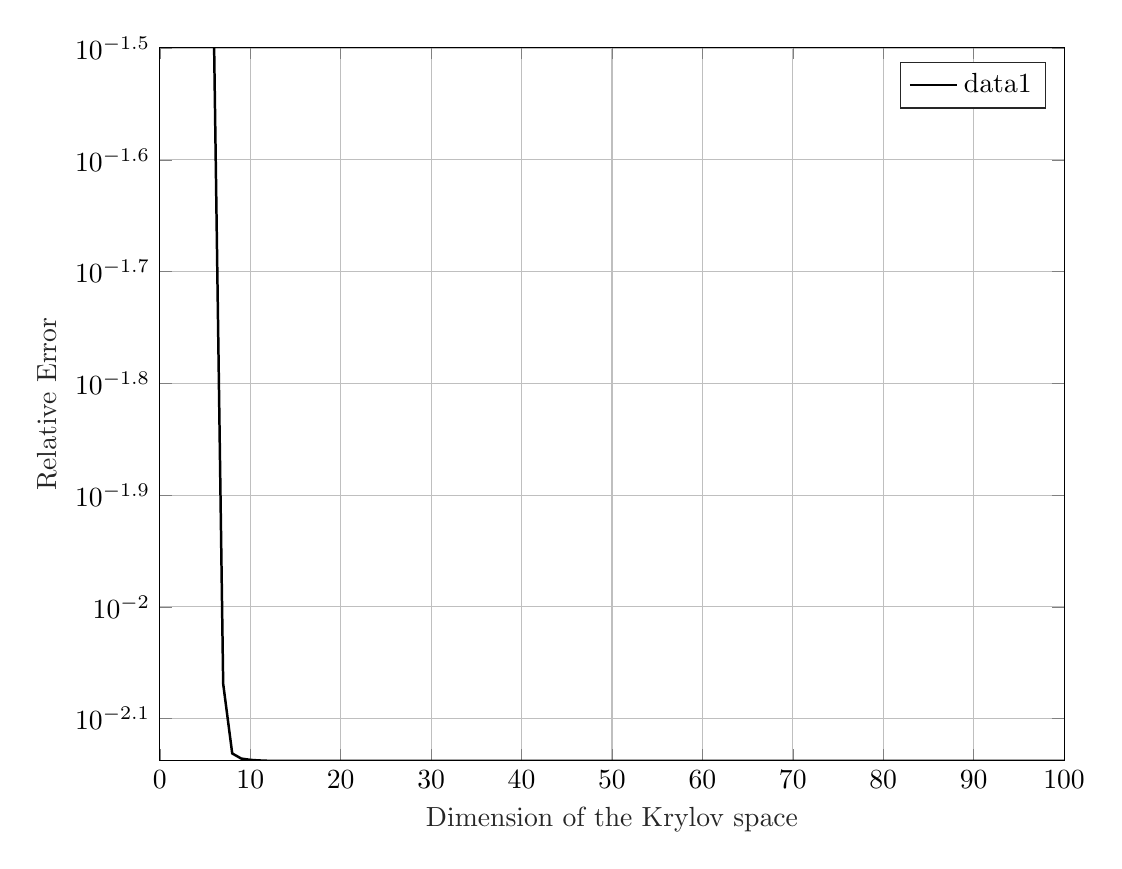
\begin{tikzpicture}

\begin{axis}[%
width=4.521in,
height=3.566in,
at={(0.758in,0.481in)},
scale only axis,
xmin=0,
xmax=100,
xlabel style={font=\color{white!15!black}},
xlabel={Dimension of the Krylov space},
ymode=log,
ymin=0.00728025449375852,
ymax=0.0316523629589043,
yminorticks=true,
ylabel style={font=\color{white!15!black}},
ylabel={Relative Error},
axis background/.style={fill=white},
xmajorgrids,
ymajorgrids,
yminorgrids,
legend style={legend cell align=left, align=left, draw=white!15!black}
]
\addplot [color=black, line width=0.9pt]
  table[row sep=crcr]{%
1	0\\
2	0\\
3	0\\
4	0\\
5	0\\
6	0.0316523629589043\\
7	0.00853323281639857\\
8	0.00739297892381665\\
9	0.00731522477074463\\
10	0.00729507382794294\\
11	0.00728688319405521\\
12	0.0072812753622548\\
13	0.00728040192286124\\
14	0.00728027966524952\\
15	0.00728025764976262\\
16	0.00728025501364829\\
17	0.0072802546250312\\
18	0.00728025450204835\\
19	0.00728025449665118\\
20	0.00728025449376016\\
21	0.00728025449397494\\
22	0.00728025449375852\\
23	0.00728025449380676\\
24	0.0072802544938222\\
25	0.00728025449382112\\
26	0.00728025449382083\\
27	0.00728025449382123\\
28	0.00728025449382118\\
29	0.00728025449382118\\
30	0.00728025449382118\\
31	0.00728025449382118\\
32	0.00728025449382118\\
33	0.00728025449382118\\
34	0.00728025449382118\\
35	0.00728025449382118\\
36	0.00728025449382118\\
37	0.00728025449382118\\
38	0.00728025449382118\\
39	0.00728025449382118\\
40	0.00728025449382118\\
41	0.00728025449382118\\
42	0.00728025449382118\\
43	0.00728025449382118\\
44	0.00728025449382118\\
45	0.00728025449382118\\
46	0.00728025449382118\\
47	0.00728025449382118\\
48	0.00728025449382118\\
49	0.00728025449382118\\
50	0.00728025449382118\\
51	0.00728025449382118\\
52	0.00728025449382118\\
53	0.00728025449382118\\
54	0.00728025449382118\\
55	0.00728025449382118\\
56	0.00728025449382118\\
57	0.00728025449382118\\
58	0.00728025449382118\\
59	0.00728025449382118\\
60	0.00728025449382118\\
61	0.00728025449382118\\
62	0.00728025449382118\\
63	0.00728025449382118\\
64	0.00728025449382118\\
65	0.00728025449382118\\
66	0.00728025449382118\\
67	0.00728025449382118\\
68	0.00728025449382118\\
69	0.00728025449382118\\
70	0.00728025449382118\\
71	0.00728025449382118\\
72	0.00728025449382118\\
73	0.00728025449382118\\
74	0.00728025449382118\\
75	0.00728025449382118\\
76	0.00728025449382118\\
77	0.00728025449382118\\
78	0.00728025449382118\\
79	0.00728025449382118\\
80	0.00728025449382118\\
81	0.00728025449382118\\
82	0.00728025449382118\\
83	0.00728025449382118\\
84	0.00728025449382118\\
85	0.00728025449382118\\
86	0.00728025449382118\\
87	0.00728025449382118\\
88	0.00728025449382118\\
89	0.00728025449382118\\
90	0.00728025449382118\\
91	0.00728025449382118\\
92	0.00728025449382118\\
93	0.00728025449382118\\
94	0.00728025449382118\\
95	0.00728025449382118\\
96	0.00728025449382118\\
97	0.00728025449382118\\
98	0.00728025449382118\\
99	0.00728025449382118\\
100	0.00728025449382118\\
};
\addlegendentry{data1}

\end{axis}
\end{tikzpicture}%
        \caption{}
        \label{fig:sign_shift_bad}
    \end{subfigure}\hspace{0.05\linewidth}
    \begin{subfigure}[b]{.45\linewidth}
        % This file was created by matlab2tikz.
%
%The latest updates can be retrieved from
%  http://www.mathworks.com/matlabcentral/fileexchange/22022-matlab2tikz-matlab2tikz
%where you can also make suggestions and rate matlab2tikz.
%
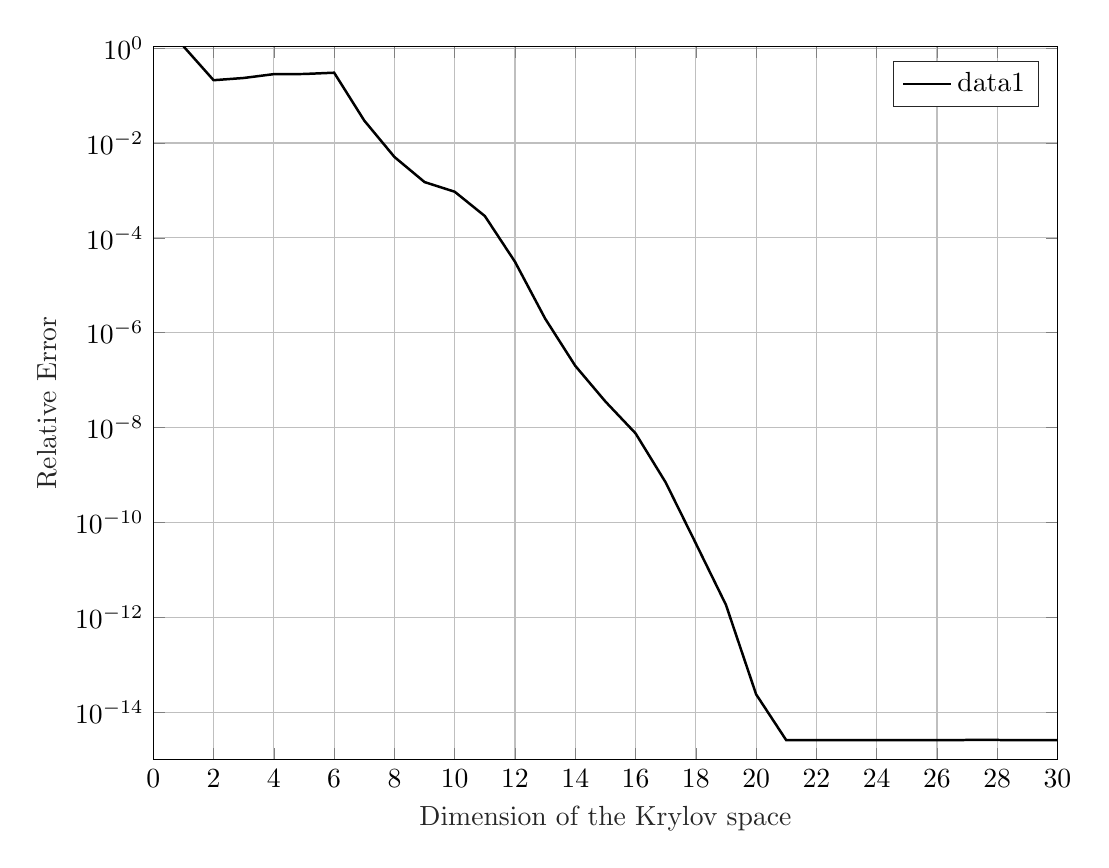
\begin{tikzpicture}

\begin{axis}[%
width=4.521in,
height=3.566in,
at={(0.758in,0.481in)},
scale only axis,
xmin=0,
xmax=30,
xlabel style={font=\color{white!15!black}},
xlabel={Dimension of the Krylov space},
ymode=log,
ymin=1e-15,
ymax=1.0936264566669,
yminorticks=true,
ylabel style={font=\color{white!15!black}},
ylabel={Relative Error},
axis background/.style={fill=white},
xmajorgrids,
ymajorgrids,
yminorgrids,
legend style={legend cell align=left, align=left, draw=white!15!black}
]
\addplot [color=black, line width=0.9pt]
  table[row sep=crcr]{%
1	1.0936264566669\\
2	0.210971251938171\\
3	0.235130155286692\\
4	0.283419469973123\\
5	0.285336085574758\\
6	0.303829845315139\\
7	0.0296699364012573\\
8	0.00507854647163762\\
9	0.00150009321797341\\
10	0.000938707425744322\\
11	0.000288484339982287\\
12	3.12969997996758e-05\\
13	1.98615828157382e-06\\
14	2.00197245255695e-07\\
15	3.53921623364422e-08\\
16	7.55132688409095e-09\\
17	6.95696803443883e-10\\
18	3.60443967049768e-11\\
19	1.82267226420508e-12\\
20	2.37324582655204e-14\\
21	2.55514325745832e-15\\
22	2.55514325745832e-15\\
23	2.55514325745832e-15\\
24	2.55514325745832e-15\\
25	2.55514325745832e-15\\
26	2.55514325745832e-15\\
27	2.58255801214404e-15\\
28	2.58255801214404e-15\\
29	2.55514325745832e-15\\
30	2.55514325745832e-15\\
};
\addlegendentry{data1}

\end{axis}
\end{tikzpicture}%
        \caption{}
        \label{fig:sign_shift_good}
    \end{subfigure}
    \caption{Same experiments as in figure \ref{fig:fullritz} using a static $\sigma=\mathbb{E}[(\lambda_1+\lambda_2)/2]$. We see that the convergence is much better than in the previous case, and that the Ritz values converge much faster in both matrices. The well-conditioned matrix (figures \ref{fig:ritz_shift_good} and \ref{fig:sign_shift_good}) also converges, but un much fewer iterations. Finally, wee see that even the very ill-conditioned matrix (figures \ref{fig:ritz_shift_bad} and \ref{fig:sign_shift_bad}) converges in only 20 iterations.}
    \label{fig:shiftritz_full}
\end{figure}
\subsubsection{Counting positive eigenvalues}
We now have an efficient arnoldi method for ill-conditioned matrices. Let us refine Algorithm 3 using the shifted invert Arnoldi method. To better assess the spectral component of the matrix, we will not use the same approach to define $\sigma$. Instead, $\sigma$ will be defined by a uniformly distributed variable such that $$\sigma\sim\mathcal{U}(lb,ub)$$ with 
\begin{equation*}
    \begin{cases}
        lb = \mathbb{E}\left[\min(\text{real}(\lambda_i))\right] \\
        ub = \mathbb{E}\left[\max(\text{real}(\lambda_i))\right]
    \end{cases}
\end{equation*}
This way, the shifted invert will, throughout the iteration, explore the whole spectrum of $\mathbf{A}$, and thus will be able to estimate the number of positive eigenvalues thanks to the convergence of the Monte-Carlo like approach. Algorithm 5 describes the new method.
\begin{algorithm2e}
    \SetAlgoLined
    \KwData{$A \in \mathbb{C}^{n \times n}$, $k \in \mathbb{N}$, $N \in \mathbb{N}$, $(lb,ub)\in\mathbb{R}^2$}
    \KwResult{$k_+ \in \mathbb{R}$}
    \caption{Corrected Computing $k_{+}(A)$}
    $\mathbf{q} \gets \mathbf{0}\in\mathbb{R}^{N}$\;
    \For{$i = 1$ \KwTo $N$}{
      $\mathbf{u} \gets \text{randn}(n, 1)$\;
      $\hat{\mathbf{u}} \gets \frac{\mathbf{u}}{\|\mathbf{u}\|}$\;
      $\sigma\gets \text{uniform}(lb,ub)$\;
      $[H, Q] \gets \text{shifted\_invert\_arnoldi}(A, \hat{\mathbf{u}}, k, \sigma)$\;
      $q(i) \gets \text{trace}(\text{sign}(H))$\;
    }
    $q_+ := \text{mode}(\mathbf{q}) $\;
    $k_+\gets (q+k)/2$
\end{algorithm2e}

In figure \ref{fig:kp}, we show the comparison between Algorithm 3 and 5. For this case, the maximum dimension of the Krylov subspace $k$ was set at 15, as we saw it provided good spectral approximation using the shifed-invert Arnoldi (figure \ref{fig:shiftritz_full}). The number of samples is fairly low, we vary this number from 1 to 20. 

\begin{figure}
    \centering
    \begin{subfigure}[b]{.45\linewidth}
        % This file was created by matlab2tikz.
%
%The latest updates can be retrieved from
%  http://www.mathworks.com/matlabcentral/fileexchange/22022-matlab2tikz-matlab2tikz
%where you can also make suggestions and rate matlab2tikz.
%
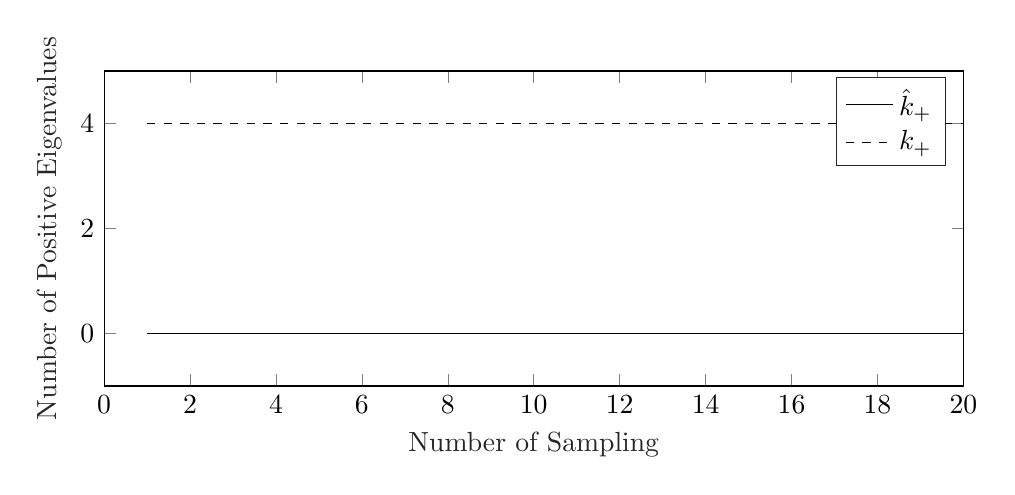
\begin{tikzpicture}

\begin{axis}[%
width=.9\linewidth,
height=4cm,
at={(0in,0in)},
scale only axis,
xmin=0,
xmax=20,
xlabel style={font=\color{white!15!black}},
xlabel={Number of Sampling},
ymin=-1,
ymax=5,
ylabel style={font=\color{white!15!black}},
ylabel={Number of Positive Eigenvalues},
axis background/.style={fill=white},
legend style={legend cell align=left, align=left, draw=white!15!black}
]
\addplot [color=black]
  table[row sep=crcr]{%
1	0\\
2	0\\
3	0\\
4	0\\
5	0\\
6	0\\
7	0\\
8	0\\
9	0\\
10	0\\
11	0\\
12	0\\
13	0\\
14	0\\
15	0\\
16	0\\
17	0\\
18	0\\
19	0\\
20	0\\
};
\addlegendentry{$\hat{k}_+$}

\addplot [color=black, dashed]
  table[row sep=crcr]{%
1	4\\
20	4\\
};
\addlegendentry{$k_+$}

\end{axis}
\end{tikzpicture}%
        \caption{}
        \label{fig:wrong_kp}
    \end{subfigure}\hspace{0.05\linewidth}
    \begin{subfigure}[b]{.45\linewidth}
        % This file was created by matlab2tikz.
%
%The latest updates can be retrieved from
%  http://www.mathworks.com/matlabcentral/fileexchange/22022-matlab2tikz-matlab2tikz
%where you can also make suggestions and rate matlab2tikz.
%
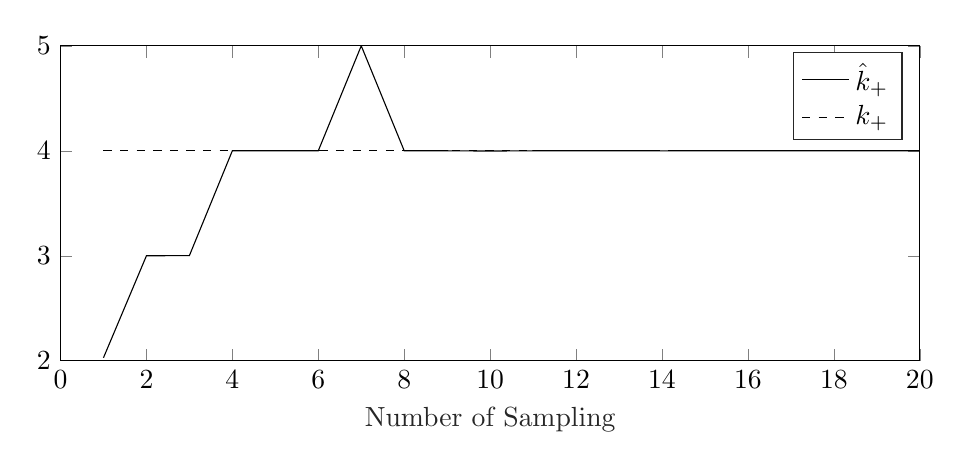
\begin{tikzpicture}

\begin{axis}[%
width=.9\linewidth,
height=4cm,
at={(0in,0in)},
scale only axis,
xmin=0,
xmax=20,
xlabel style={font=\color{white!15!black}},
xlabel={Number of Sampling},
ymin=2,
ymax=5,
ylabel style={font=\color{white!15!black}},
%ylabel={Number of Positive Eigenvalues},
axis background/.style={fill=white},
legend style={legend cell align=left, align=left, draw=white!15!black}
]
\addplot [color=black]
  table[row sep=crcr]{%
1	2.02878333228051\\
2	3.00000412526795\\
3	3.00194629230602\\
4	4.00051449032303\\
5	3.99998363733881\\
6	4.00013569715796\\
7	4.99994381698126\\
8	4.00000796483248\\
9	4.00001514241167\\
10	3.99769291363055\\
11	4.00000101918524\\
12	3.99998931573416\\
13	4.00031626976621\\
14	3.99993739195579\\
15	4.00000679714354\\
16	3.99999350520674\\
17	3.99999827766674\\
18	4.000001796798\\
19	4.00000216695133\\
20	4.00016721827853\\
};
\addlegendentry{$\hat{k}_+$}

\addplot [color=black, dashed]
  table[row sep=crcr]{%
1	4\\
20	4\\
};
\addlegendentry{$k_+$}

\end{axis}
\end{tikzpicture}%
        \caption{}
        \label{fig:correct_kp}
    \end{subfigure}
    \caption{Comparison of the estimation of $k_p$ with Algorithm 3 and 5. We see that Algorithm 3 (figure \ref{fig:wrong_kp}) does not manage to find any positive eigenvalues. It uses the standard Arnoldi method, and we saw previously that it was not converging. Whereas Algorithm 5 (figure \ref{fig:correct_kp}) finds the correct value of $k_p$ very quickly. $\hat{k}_+$ (continuous line) is the estimated value of $k_+$, and $k_+$ (dashed line) is the true value of $k_+$.}
    \label{fig:kp}
\end{figure}

We conclude that, assuming a good knowledge of the spectral properties of $\mathbf{A}$ (here, the bounds of its spectrum) enables for faster and more precise computations. In this case, it allows for quick assessment of a system's stability, which is a very important property in control theory.
\printbibliography
\end{document}